\documentclass{article}
\usepackage{graphicx}
\usepackage{float}
\usepackage[utf8]{vietnam}
\usepackage{lipsum}
\usepackage{tikz}
\usepackage{tikzpagenodes}
\usetikzlibrary{calc}
\usepackage[a4paper, top=2cm, bottom=2cm, left=3.5cm, right=2.5cm]{geometry}
\usepackage{pdfpages}
\usepackage{hyperref}
\usepackage{amsmath}
\usepackage{enumitem} % Gói hỗ trợ tùy chỉnh danh sách
\usepackage{xcolor}
\usepackage{tcolorbox} % Gói hỗ trợ tùy chỉnh khung
\usepackage{makecell} % Gói hỗ trợ tạo ô trong bảng
\usepackage{longtable} % Gói hỗ trợ bảng dài nhiều trang
% \usetikzlibrary{arrows.meta}
% \usepackage{rotating} % Bắt buộc phải có
% \usepackage{pdflscape} % Khuyên dùng pdflscape thay vì lscape để PDF xoay đúng chiều khi xem trên máy tính

\setlength{\parindent}{0pt} % Không thụt lề

\definecolor{RedHUST}{RGB}{205,5,5}
% \setlist{format={\color{RedHUST}\bfseries}} % Đặt màu cho danh sách

% Định nghĩa lại lệnh \lipsum gốc để tự động bọc trong màu RedHUST
\let\oldlipsum\lipsum
\renewcommand{\lipsum}[1][1-7]{{\color{RedHUST}\oldlipsum[#1]}}

\definecolor{BlueSAMI}{RGB}{1,90,143}
\setlist{format={\color{BlueSAMI}\bfseries}} % Đặt màu cho danh sách

% Định nghĩa môi trường block
\newenvironment{block}[1]
{\begin{tcolorbox}[%
colback=white, % Màu nền nội dung
colframe=BlueSAMI, % Màu khung
arc=3mm, % Góc bo tròn
title={\textbf{#1}}, % Tiêu đề, in đậm
colbacktitle=BlueSAMI, % Màu nền tiêu đề
coltitle=white, % Màu chữ tiêu đề
boxrule=2pt, % Độ dày của khung
before upper={\tcbtitle\vskip0pt\par}
]
\begin{minipage}{\textwidth}}
{\end{minipage}
\end{tcolorbox}}

\setlength{\headheight}{12.42429pt} % bug header foooter
\usepackage{fancyhdr}
\pagestyle{fancy}
\lhead{Đồ án tốt nghiệp}
\rhead{Vũ Văn Nghĩa - 20206205}
\renewcommand{\headrulewidth}{0.4pt}
\renewcommand{\footrulewidth}{0.4pt}

% Căn giữa tiêu đề mục lục
\makeatletter
\renewcommand{\tableofcontents}{
\begin{center}
\section*{\contentsname}
\end{center}
\@starttoc{toc}
}
\makeatother

\numberwithin{figure}{section} % Đặt số ảnh theo section
% Căn giữa tiêu đề danh sách hình ảnh
\makeatletter
\renewcommand{\listoffigures}{
\begin{center}
\section*{\listfigurename}
\end{center}
\@starttoc{lof}
}
\makeatother

% \usepackage{microtype}
% \usepackage{blindtext}

% \usepackage{etoolbox}
% \pretocmd{\section}{\clearpage}{}{}
\usepackage{csquotes}

% Tự động thêm chữ "CHƯƠNG" vào trước số section và định dạng lại các đề mục con
\usepackage{titlesec}
\renewcommand{\thesection}{CHƯƠNG \arabic{section}}
\renewcommand{\thesubsection}{\arabic{section}.\arabic{subsection}}
\renewcommand{\thesubsubsection}{\thesubsection.\arabic{subsubsection}}
\renewcommand{\thefigure}{\arabic{section}.\arabic{figure}}
\renewcommand{\thetable}{\arabic{section}.\arabic{table}}

% Định dạng hiển thị tiêu đề Chương (section) trong văn bản
\titleformat{\section}[block]
{\normalfont\Large\bfseries\centering} % Căn giữa, chữ in đậm, cỡ lớn
{\thesection.} % Nhãn hiển thị (ví dụ: CHƯƠNG 1.)
{1em} % Khoảng cách giữa nhãn và tiêu đề chương
{}

% Cấu hình Mục lục (TOC) tránh lỗi tràn lề và đè chữ khi thêm chữ "CHƯƠNG" viết hoa
\usepackage[titles]{tocloft}
\setlength{\cftsecnumwidth}{7.0em} % Độ rộng cột số hiệu Section (đủ chỗ cho CHƯƠNG X.)
\setlength{\cftsubsecindent}{7.0em} % Thụt lề Subsection thẳng hàng với tiêu đề Section (7.0em)
\setlength{\cftsubsecnumwidth}{3.0em} % Độ rộng cột số hiệu Subsection
\setlength{\cftsubsubsecindent}{10.0em} % Thụt lề Subsubsection (7.0 + 3.0)
\setlength{\cftsubsubsecnumwidth}{3.5em} % Độ rộng cột số hiệu Subsubsection

\newif\ifdev
% Chọn 1 trong 2 dòng dưới đây để bật/tắt chế độ:
\devtrue % BẬT chế độ Dev
% \devfalse % TẮT chế độ Dev (Production)

\ifdev
\pagecolor{black} % Thiết lập nền toàn bộ trang PDF thành màu đen
\color{white} % Thiết lập màu chữ mặc định toàn trang là trắng
\fi

\begin{document}

% % % % % \section{Bài toán nghiệp vụ}

% % % % \begin{frame}{Sự cần thiết}

\begin{itemize}

\item Hệ thống pháp luật rất phức tạp

\item Cá nhân, doanh nghiệp bỏ lỡ cập nhật

\end{itemize}

\begin{figure}[H]
\centering

\includegraphics[width=\linewidth,height=0.55\textheight,keepaspectratio]{pictures/chatbot-tra-cuu-luat-la-gi.jpeg}
\caption[AI hỗ trợ tư vấn pháp luật]{AI hỗ trợ tư vấn pháp luật (Nguồn: \footnotemark)}
\end{figure}
\footnotetext{\url{https://vnptai.io/vi/blog/detail/chatbot-ai-tra-cuu-luat}}

\note{

Hệ thống pháp luật rất phức tạp.

\hrule

Các VBPL có thể thay thế, bổ sung VBPL khác,

hoặc bị hết hiệu lực.

\hrule

Nếu cá nhân, doanh nghiệp bỏ lỡ cập nhật

Và vô tình áp dụng sai luật

\hrule

=> Dẫn đến hậu quả tài chính và rủi ro pháp lý

}

\end{frame}

% hệ thống pháp luật rất phức tạp.

% các văn bản pháp luật có thể thay thế, bổ sung văn bản pháp luật khác

% hoặc bị hết hiệu lực. nếu cá nhân, doanh nghiệp bỏ lỡ cập nhật

% và vô tình áp dụng sai luật. dẫn đến hậu quả tài chính và rủi ro pháp lý


% % % % \begin{frame}{Vai trò và chức năng}
\begin{table}
\centering
\caption{Bảng vai trò và chức năng trong hệ thống} % <-- Lệnh caption được thêm ở đây

% Bây giờ cả hai cột đều có thể dùng 'l' (căn trái) hoặc 'c' (căn giữa)
\begin{tabular}{|l|l|}
\hline
\textbf{Vai trò} & \textbf{Chức năng} \\
\hline

% Dòng 1: Guest
Guest &
\makecell[l]{ % [l] để căn trái các dòng bên trong ô
Giới thiệu, nghe thử giọng nói, xem gói VIP \\
Đăng ký email,
Đăng nhập \textbf{
\textcolor{blue}{G}%
\textcolor{red}{o}%
\textcolor{yellow}{o}%
\textcolor{blue}{g}%
\textcolor{green}{l}%
\textcolor{red}{e}
}
} \\
\hline

% Dòng 2: User
User &
\makecell[l]{
Đăng nhập và quản lý tài khoản, cài đặt \\
Thực hiện trò chuyện, đánh dấu và chia sẻ \\
Mua gói VIP và xem lịch sử
} \\
\hline

% Dòng 3: VIP
VIP &
\makecell[l]{
Suy luận nâng cao\\
Tài liệu cá nhân \\
Sử dụng giọng nói
} \\
\hline

% Dòng 4: Admin
Admin &
\makecell[l]{
Quản lý nhân vật,
gói VIP \\
Báo cáo đường ống dữ liệu
} \\
\hline
\end{tabular}
\end{table}
\end{frame}


% % % % \begin{frame}{Sơ đồ Use Case - Khách vãng lai}
\begin{figure}[H]
\centering
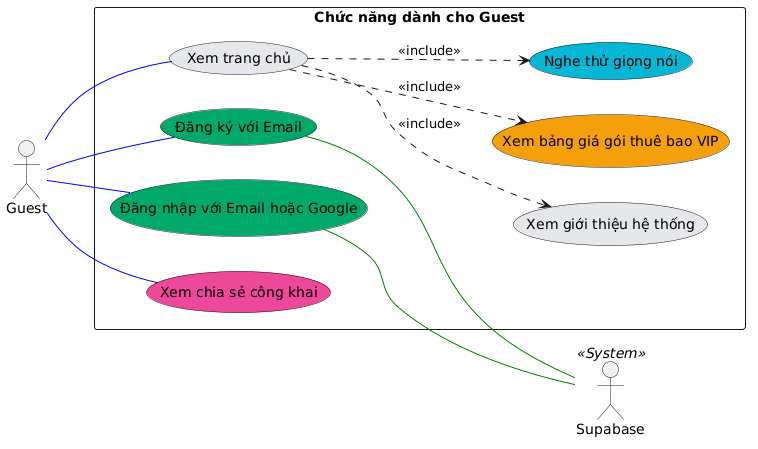
\includegraphics[width=\linewidth,height=0.74\textheight,keepaspectratio]{pictures/UML-UseCase-Guest.png}
\caption{Sơ đồ Use Case chức năng của khách vãng lai}
\end{figure}

\note{

dưới đây là sơ đồ iu cây dành cho người dùng trong hệ thống
\hrule

đầu tiên là khách vãng lai (chưa đăng nhập hệ thống)
\hrule

tiếp theo sơ đồ iu cây dành cho người dùng cơ bản (đã đăng nhập)
\hrule

tiếp theo sơ đồ iu cây dành cho người dùng vip
\hrule

cuối cùng là sơ đồ iu cây dành cho quản trị viên (admin)

}
\end{frame}

% % % % \begin{frame}{Sơ đồ Use Case - Người dùng cơ bản}
\begin{figure}[H]
\centering
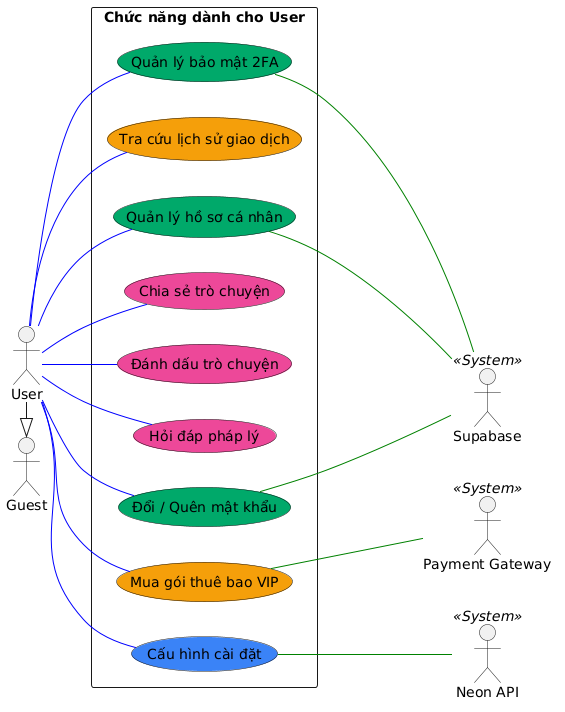
\includegraphics[width=\linewidth,height=0.74\textheight,keepaspectratio]{pictures/UML-UseCase-User.png}
\caption{Sơ đồ Use Case chức năng của người dùng cơ bản}
\end{figure}

\note{

Dưới đây là

Sơ đồ Use Case
chi tiết

dành cho người dùng cơ bản
(đã đăng nhập).

}
\end{frame}

% % % % \begin{frame}{Sơ đồ Use Case - Người dùng VIP}
\begin{figure}[H]
\centering
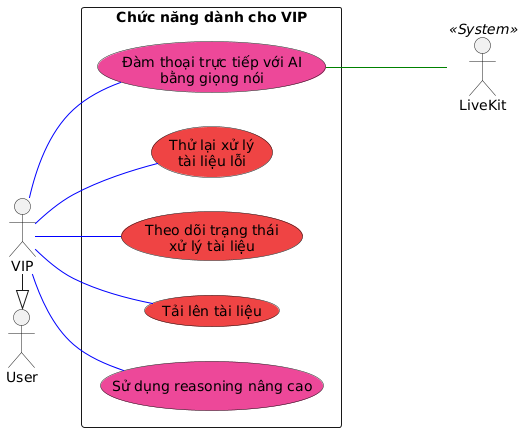
\includegraphics[width=\linewidth,height=0.74\textheight,keepaspectratio]{pictures/UML-UseCase-VIP.png}
\caption{Sơ đồ Use Case chức năng của người dùng VIP}
\end{figure}

\note{

Dưới đây là

Sơ đồ Use Case
chi tiết

dành cho nhóm người dùng VIP.

}
\end{frame}

% % % % \begin{frame}{Sơ đồ Use Case - Quản trị viên}
\begin{figure}[H]
\centering
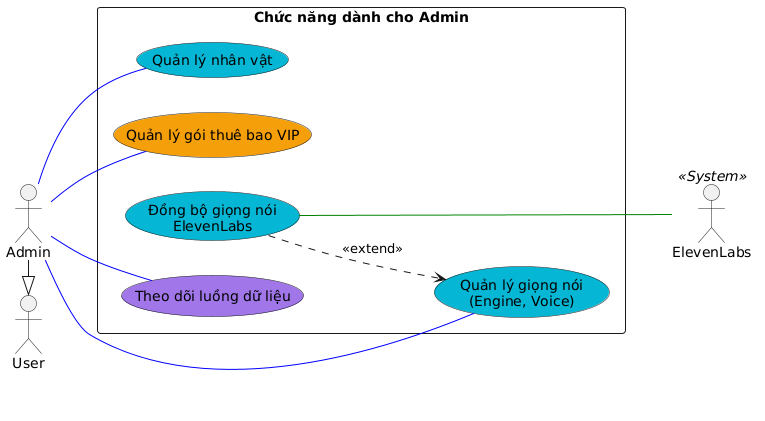
\includegraphics[width=\linewidth,height=0.72\textheight,keepaspectratio]{pictures/UML-UseCase-Admin.png}
\caption{Sơ đồ Use Case chức năng của quản trị viên}
\end{figure}

\note{
Sơ đồ Use Case dành cho quản trị viên (Admin).
Quản trị viên có các quyền hạn cao nhất trong hệ thống bao gồm: quản lý danh sách người dùng, quản lý cấu hình các gói thanh toán VIP, giám sát hệ thống, xem các báo cáo thống kê giao dịch và quản lý các tài liệu pháp luật chung trong CSDL tri thức của hệ thống.
}
\end{frame}


% % % \section{Xây dựng hệ thống AI}
% % % \subsection{Đường ống dữ liệu}

% % % \begin{frame}{Đường ống dữ liệu văn bản pháp luật (VBPL)}
\begin{figure}[H]
\centering
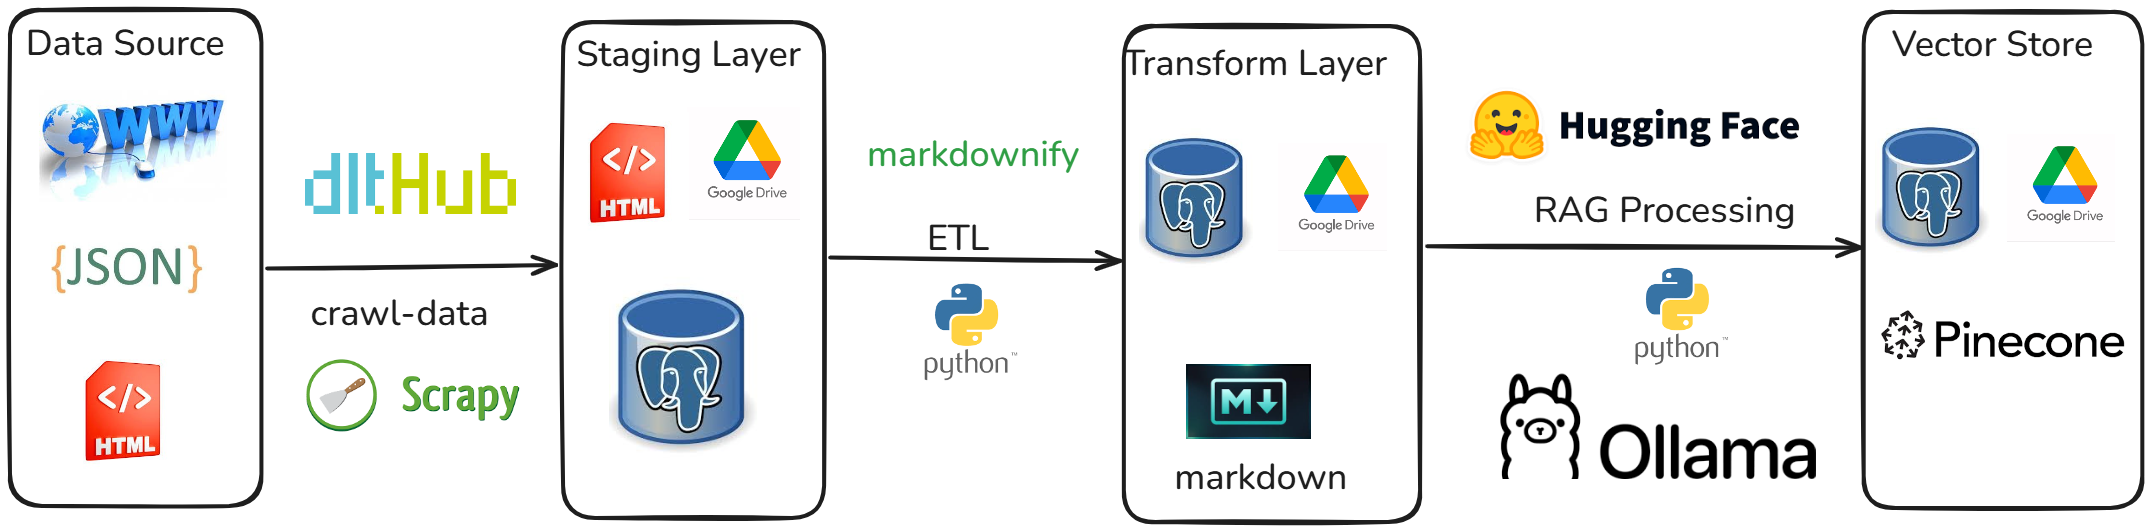
\includegraphics[height=0.55\textheight,width=0.9\textwidth,keepaspectratio]{pictures/Data-Pipeline-VBPL.excalidraw.png}
\caption{Sơ đồ tổng quan luồng dữ liệu văn bản pháp luật mới}
\end{figure}

\note{
Do nguồn dữ liệu Văn bản pháp luật Việt Nam (VBPL) thay đổi cấu trúc trang web và API vào tháng 5/2026, dự án đã xây dựng lại đường ống dữ liệu mới.
Đường ống dữ liệu này tự động hóa quy trình từ thu thập thông tin qua crawler, lưu trữ dữ liệu thô vào PostgreSQL, thực hiện tiền xử lý văn bản pháp luật và cuối cùng là tích hợp vào RAG pipeline để cập nhật CSDL tri thức của trợ lý ảo.
}
\end{frame}

% % % \begin{frame}{Quy trình các bước thu thập dữ liệu văn bản pháp luật}
\begin{figure}[H]
\centering
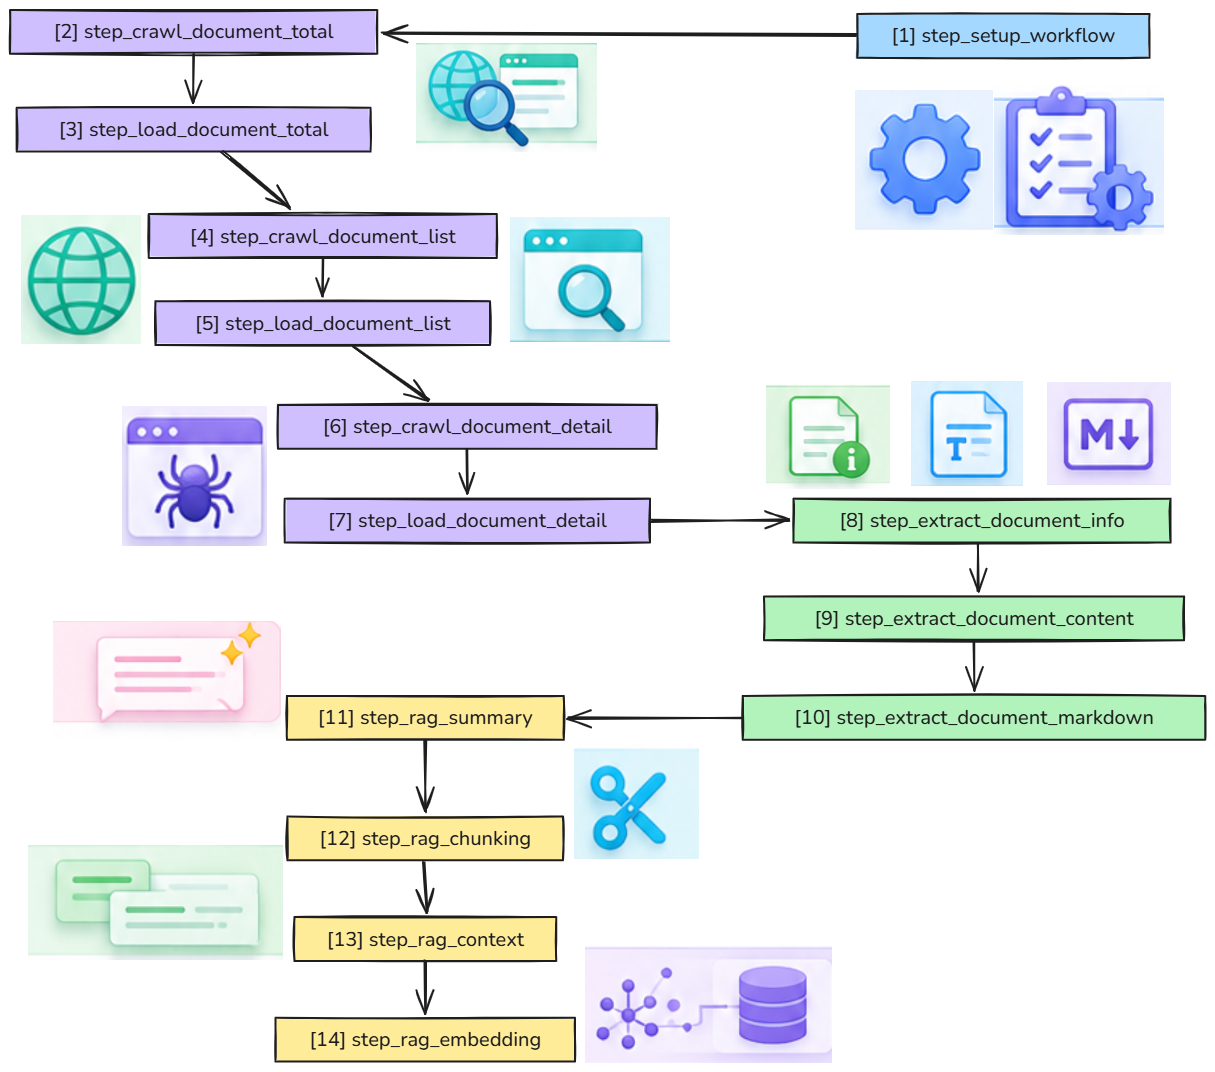
\includegraphics[height=0.55\textheight,width=0.9\textwidth,keepaspectratio]{pictures/step0.excalidraw.png}
\caption{Sơ đồ các bước thực hiện của quy trình cũ}
\end{figure}

\note{
Sơ đồ chi tiết các bước thực hiện trong quy trình cũ của đường ống dữ liệu văn bản pháp luật.
Quy trình được chia thành 3 giai đoạn: Khởi tạo luồng công việc (\texttt{step\_setup\_workflow}), thu thập tổng số lượng tài liệu (\texttt{step\_crawl\_document\_total}), tải nội dung chi tiết và cuối cùng là xử lý định dạng văn bản để chuẩn bị cho việc trích xuất thông tin.
}
\end{frame}

% % % \begin{frame}{Các bước trong đường ống dữ liệu VBPL mới}
\begin{figure}[H]
\centering
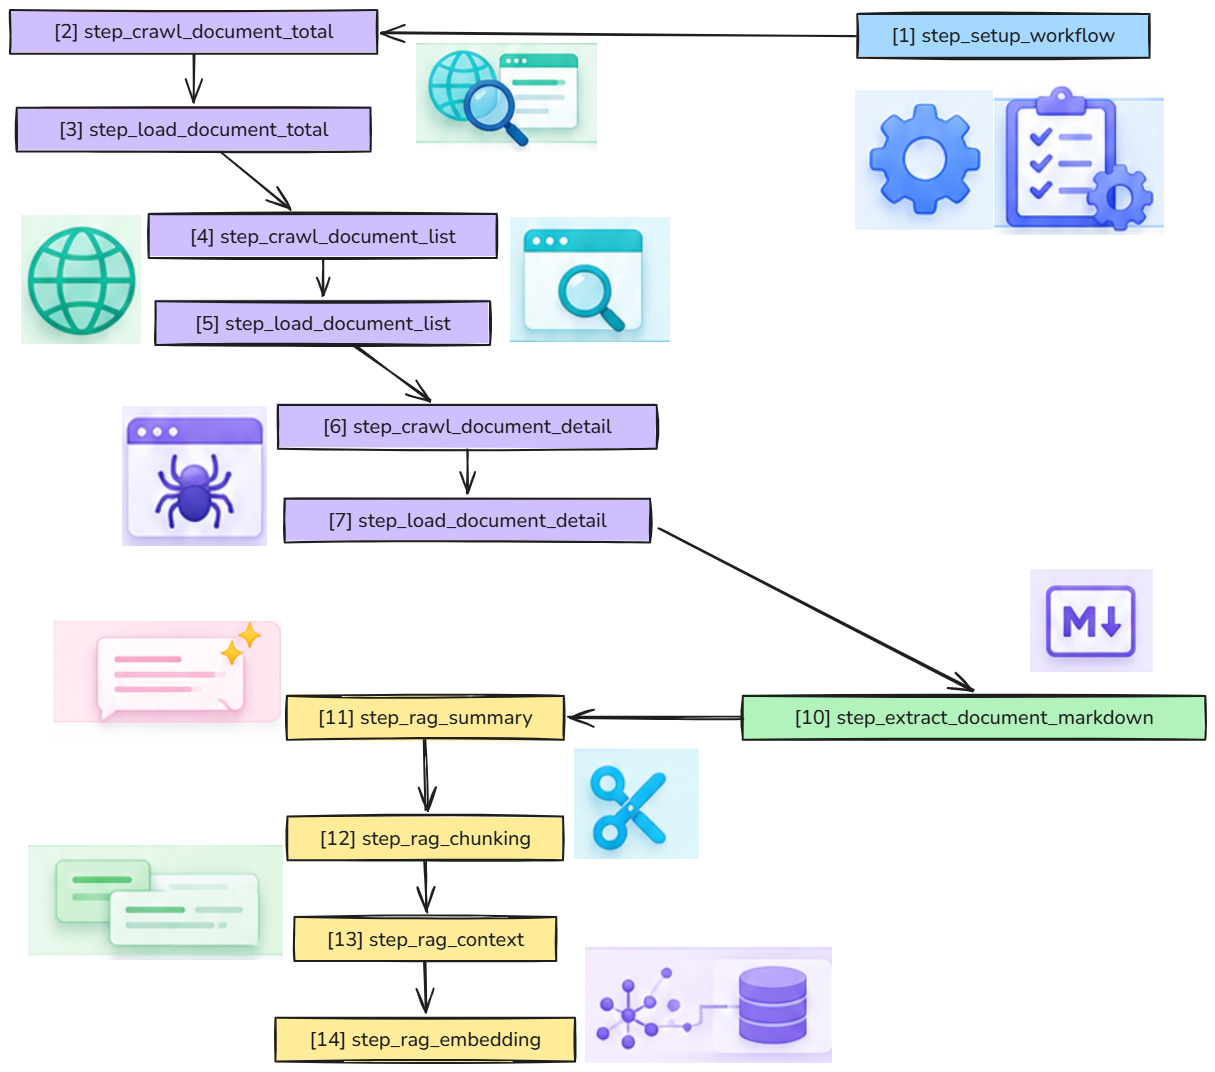
\includegraphics[height=0.7\textheight,width=0.9\textwidth,keepaspectratio]{pictures/step1.excalidraw.png}
\caption{Sơ đồ các bước thực hiện của quy trình mới}
\end{figure}

\note{
do api => bỏ bước

Sơ đồ các bước thực hiện của quy trình mới
}
\end{frame}

% % % \begin{frame}{Đường ống dữ liệu Pháp Điển}
\begin{figure}[H]
\centering
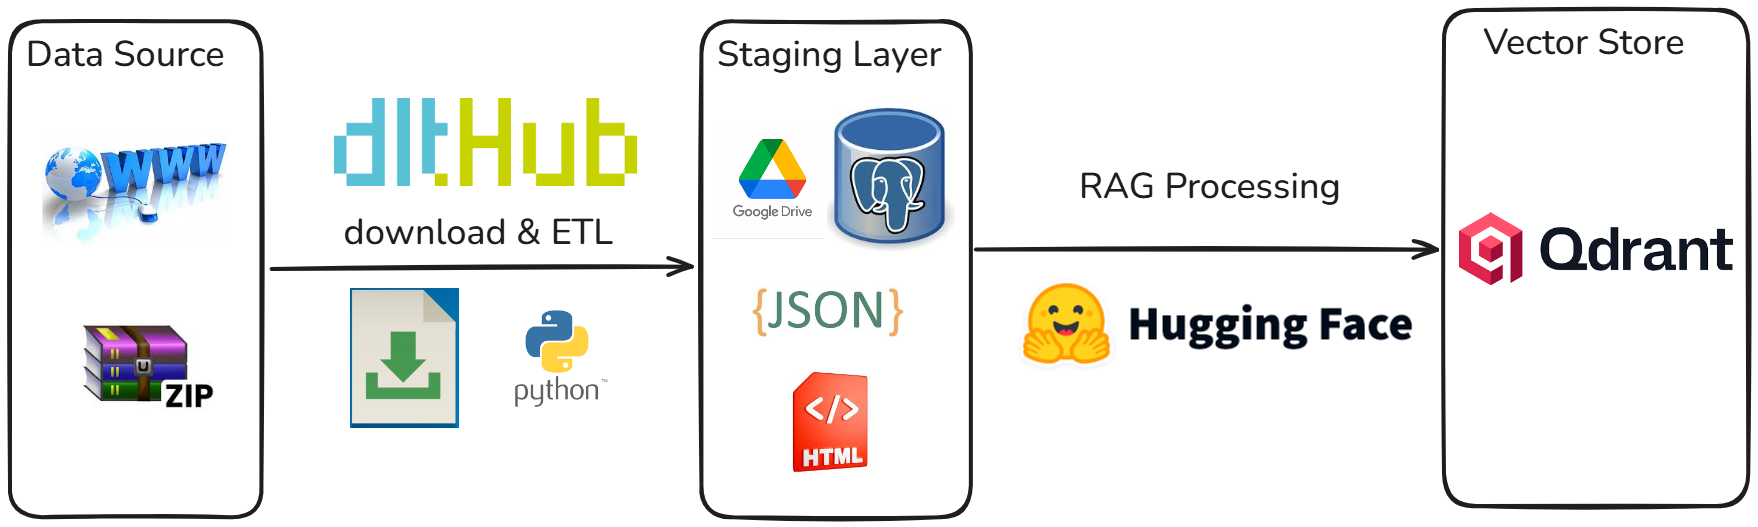
\includegraphics[height=0.55\textheight,width=0.9\textwidth,keepaspectratio]{pictures/Data-Pipeline-PhapDien.excalidraw.png}
\caption{Sơ đồ tổng quan đường ống dữ liệu Pháp Điển}
\end{figure}

\note{
Bên cạnh VBPL, hệ thống còn tích hợp Bộ Pháp Điển Việt Nam. Sơ đồ này mô tả đường ống dữ liệu Pháp Điển.
Dữ liệu Pháp Điển được tải về dưới dạng file nén ZIP từ Cổng thông tin điện tử Pháp Điển, sau đó được giải nén, chuyển đổi cấu trúc cây đề mục sang định dạng JSON, tải lên lưu trữ trên Google Drive và thực hiện vector hóa để lưu vào Vector Database.
}
\end{frame}

% % % \begin{frame}{Các bước trong đường ống dữ liệu Pháp Điển}

\begin{figure}[H]
\centering
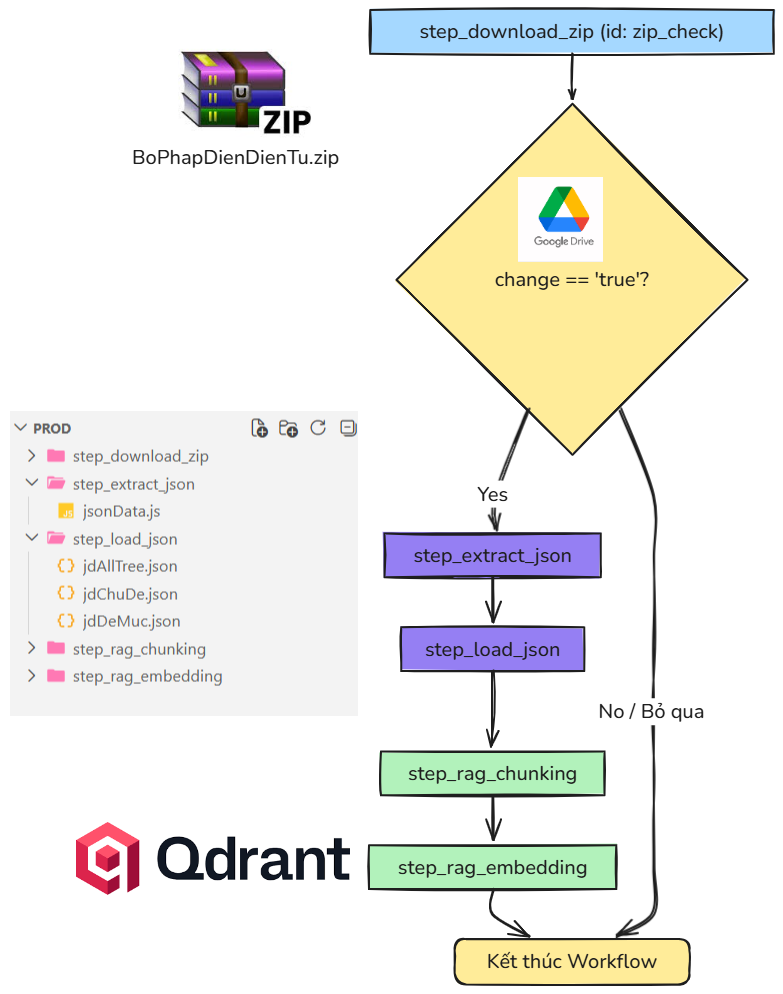
\includegraphics[height=0.7\textheight,width=0.9\textwidth,keepaspectratio]{pictures/step3.excalidraw.png}
\caption{Sơ đồ các bước thực hiện của đường ống dữ liệu Pháp Điển}
\end{figure}

\note{
Sơ đồ mô tả quy trình từng bước của đường ống dữ liệu Pháp Điển.
Quy trình bắt đầu từ việc tải file ZIP tự động (\texttt{step\_download\_zip}), tính toán mã băm MD5 để kiểm tra sự thay đổi dữ liệu so với phiên bản trước, giải nén và trích xuất cấu trúc đề mục ra các file JSON riêng biệt, sau đó chạy các tác vụ phân tích cấu trúc và lưu kết quả vector hóa.
}
\end{frame}


% % % \subsection{Agentic RAG với LangGraph}

% % % \begin{frame}{Kiến trúc Agentic RAG bằng LangGraph}
\begin{figure}[H]
\centering
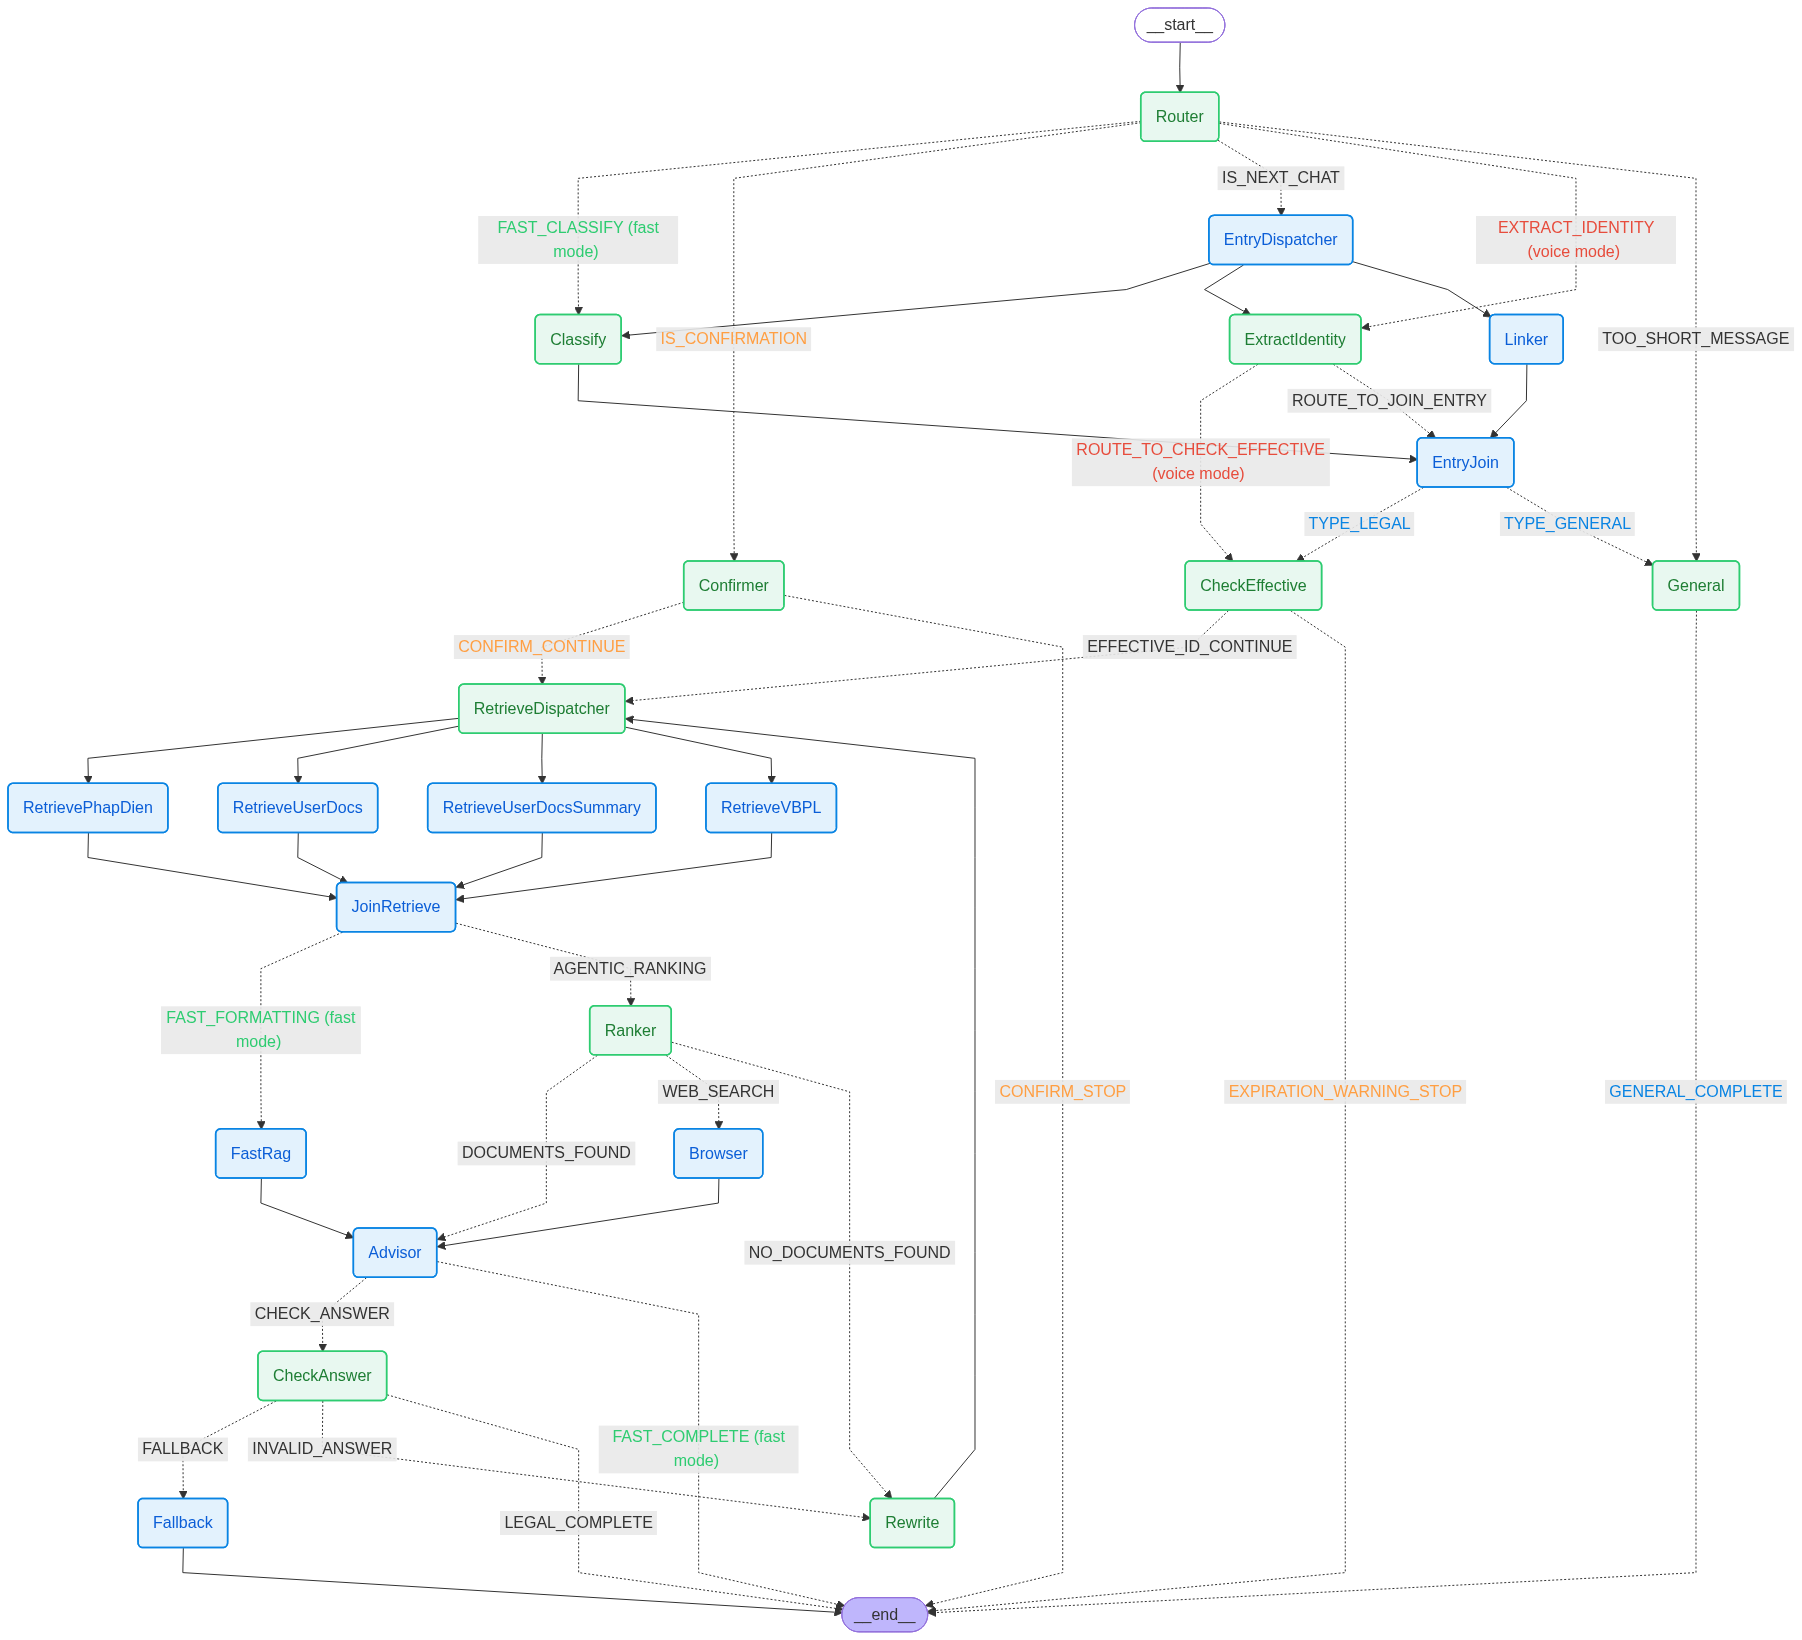
\includegraphics[height=0.55\textheight,width=0.9\textwidth,keepaspectratio]{pictures/rag_diagram.png}
\caption{Sơ đồ LangGraph của dự án}
\end{figure}

\note{
Đây là sơ đồ Agentic RAG của dự án được xây dựng bằng LangGraph. Hệ thống phân chia thông minh giữa mô hình nhỏ cho luồng cơ bản (màu xanh lá) và mô hình lớn cho các tác vụ suy luận phức tạp (màu xanh dương) để tối ưu chi phí và độ trễ.
Mỗi tin nhắn đi qua Router để kiểm tra điều kiện và định tuyến qua các node như rewrite query, retrieve tài liệu và sinh câu trả lời.
}
\end{frame}


% % % \begin{frame}{Tổng quan các dịch vụ}
\begin{figure}[H]
\centering
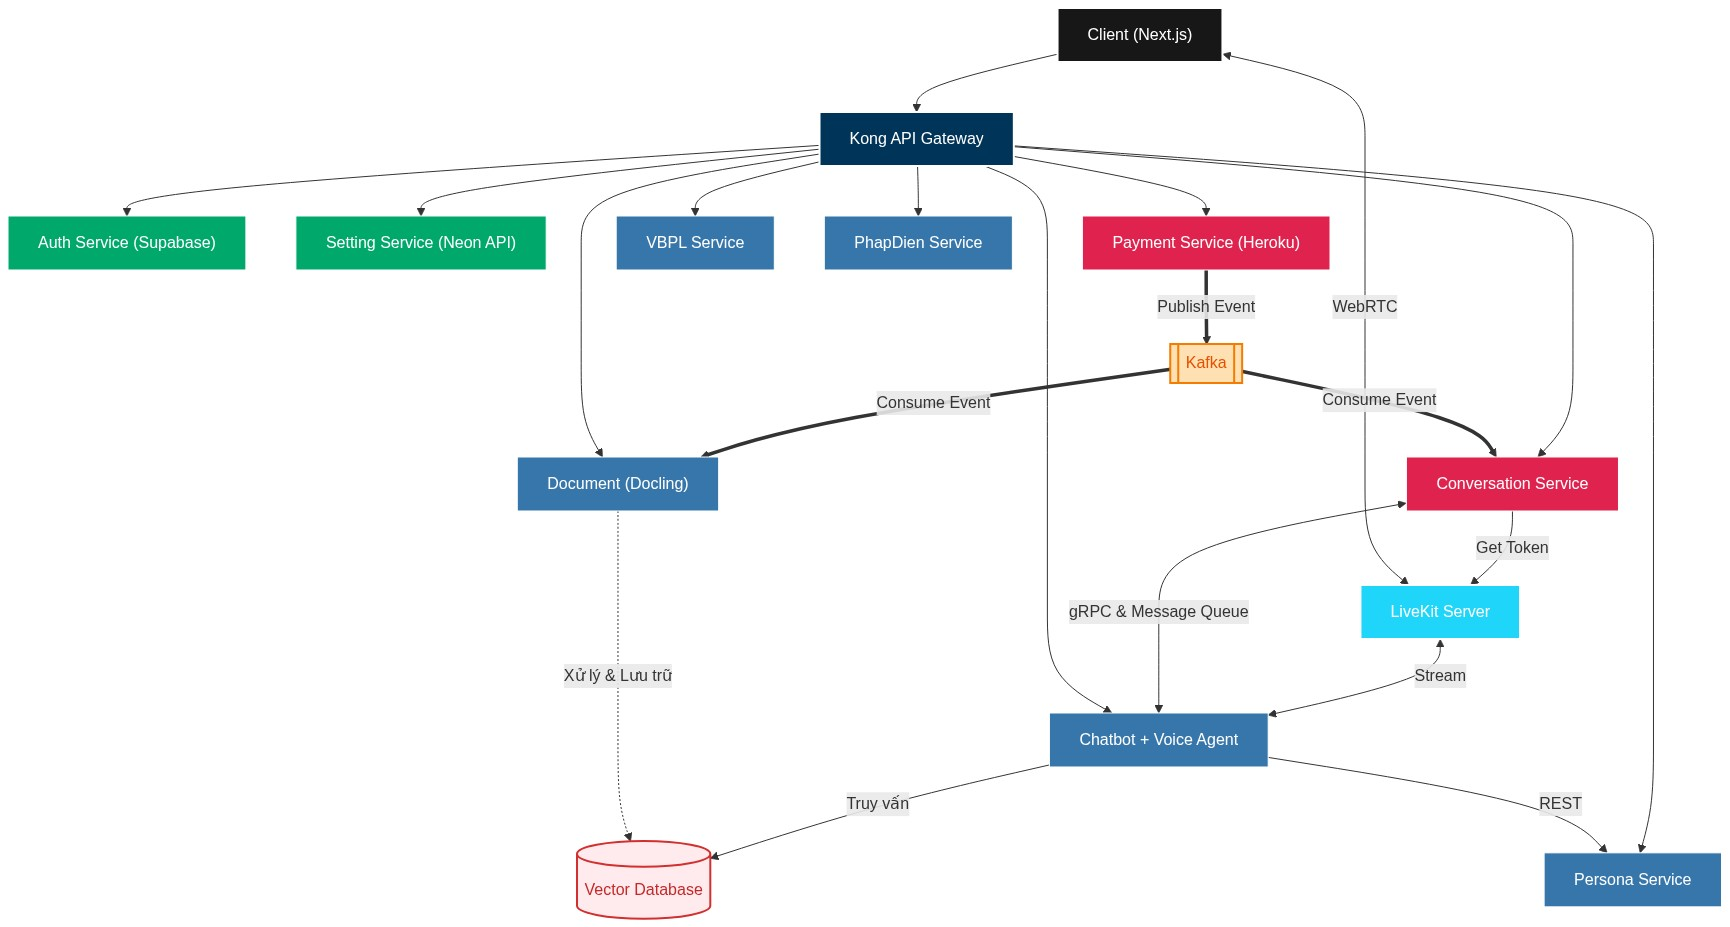
\includegraphics[height=0.7\textheight,width=0.9\textwidth,keepaspectratio]{pictures/MSA.png}
\caption{Tổng quan các dịch vụ của dự án}
\end{figure}

\note{
Sơ đồ tổng quan về kiến trúc các vi dịch vụ được triển khai trong dự án này.
Hệ thống được chia thành nhiều dịch vụ chuyên biệt như: Auth Service (xác thực), Document Service (quản lý tài liệu), Conversation Service (quản lý trò chuyện), Chatbot Service (trí tuệ nhân tạo) và Payment Service (thanh toán). Các dịch vụ này giao tiếp với nhau qua gRPC, REST API hoặc thông điệp bất đồng bộ qua Kafka/RabbitMQ.
}
\end{frame}
% nếu python cash => thanh toán , đăng nhập vẫn không sao

% Nếu các Microservice luôn để xuống service thanh toán


% % \section{Chi tiết các dịch vụ}

% % \begin{frame}{Kiến trúc Dịch vụ Thanh toán (Payment Service)}
\begin{figure}[H]
\centering
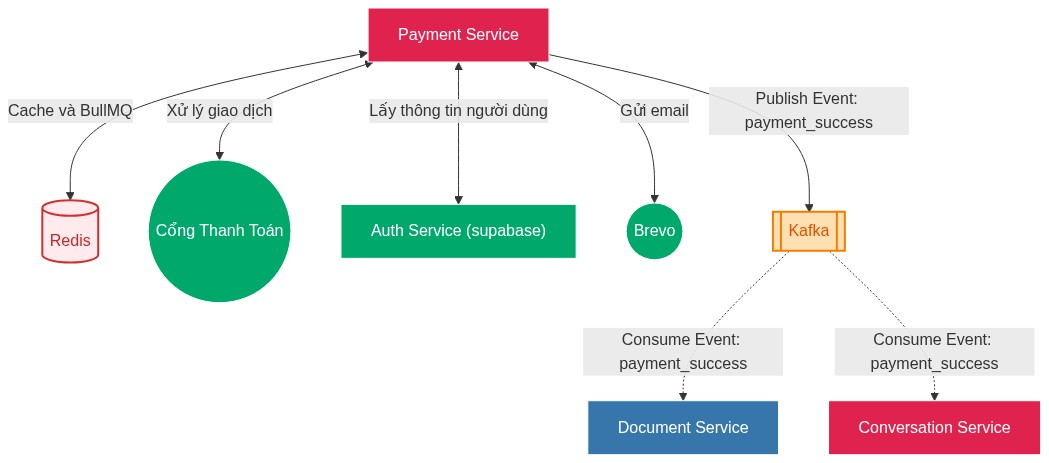
\includegraphics[height=0.7\textheight,width=0.9\textwidth,keepaspectratio]{pictures/payment-kafka-event.png}
\caption{Sơ đồ tổng quan dịch vụ thanh toán}
\end{figure}

\note{
Dịch vụ thanh toán (Payment Service) chịu trách nhiệm quản lý thông tin các gói dịch vụ (Plans), quản lý thuê bao người dùng (Subscriptions) và tích hợp với cổng thanh toán ngoại vi.
Khi người dùng thực hiện thanh toán thành công, dịch vụ này sẽ phát đi sự kiện \texttt{payment\_success} vào hệ thống truyền tin nhắn Kafka để các dịch vụ khác như Chatbot và Document cập nhật quyền VIP cho người dùng.
}
\end{frame}


% % \begin{frame}{Dịch vụ Tài liệu (Document Service)}
\begin{figure}[H]
\centering
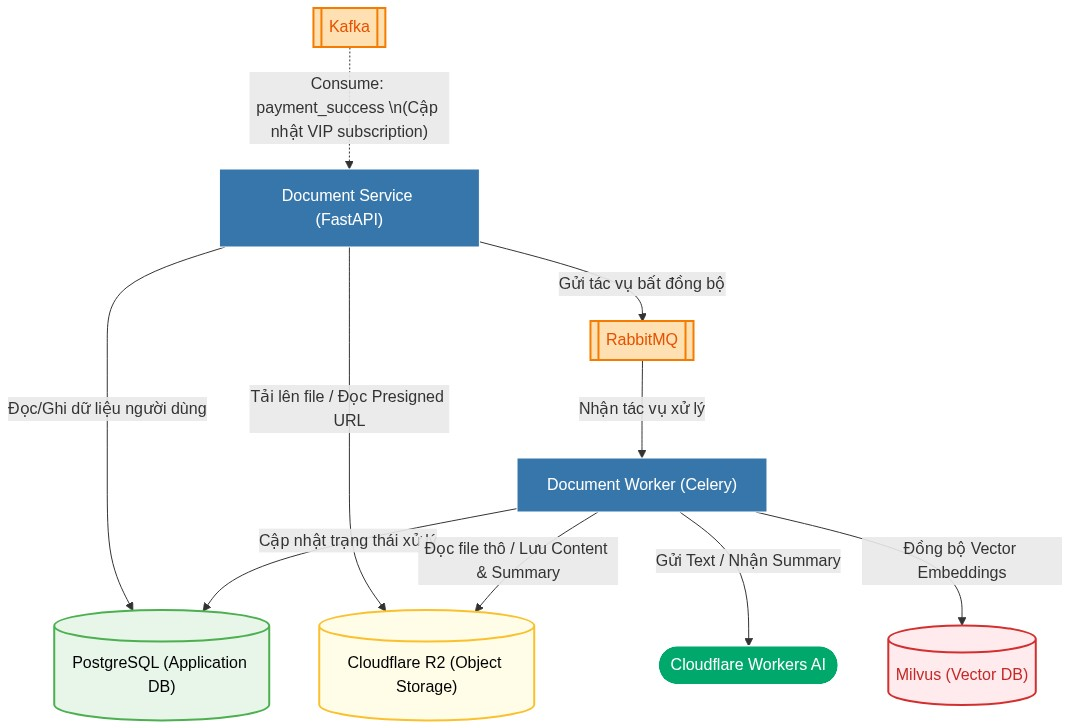
\includegraphics[height=0.7\textheight,width=0.9\textwidth,keepaspectratio]{pictures/document-overview.png}
\caption{Sơ đồ tổng quan dịch vụ văn bản}
\end{figure}

\note{
Dịch vụ tài liệu (Document Service) tiếp nhận, lưu trữ và quản lý tài liệu do người dùng VIP tải lên.
Khi nhận được tệp tin (PDF, DOCX), dịch vụ sẽ gửi yêu cầu xử lý bất đồng bộ thông qua RabbitMQ tới Document Worker. Tài liệu sẽ được trích xuất nội dung sang định dạng Markdown, tự động tóm tắt nội dung chính và tiến hành vector hóa để lưu trữ vào Vector Database Milvus phục vụ cho việc hỏi đáp trên tài liệu.
}
\end{frame}


% % \begin{frame}{Dịch vụ Chatbot và Trò chuyện}
\begin{figure}[H]
\centering
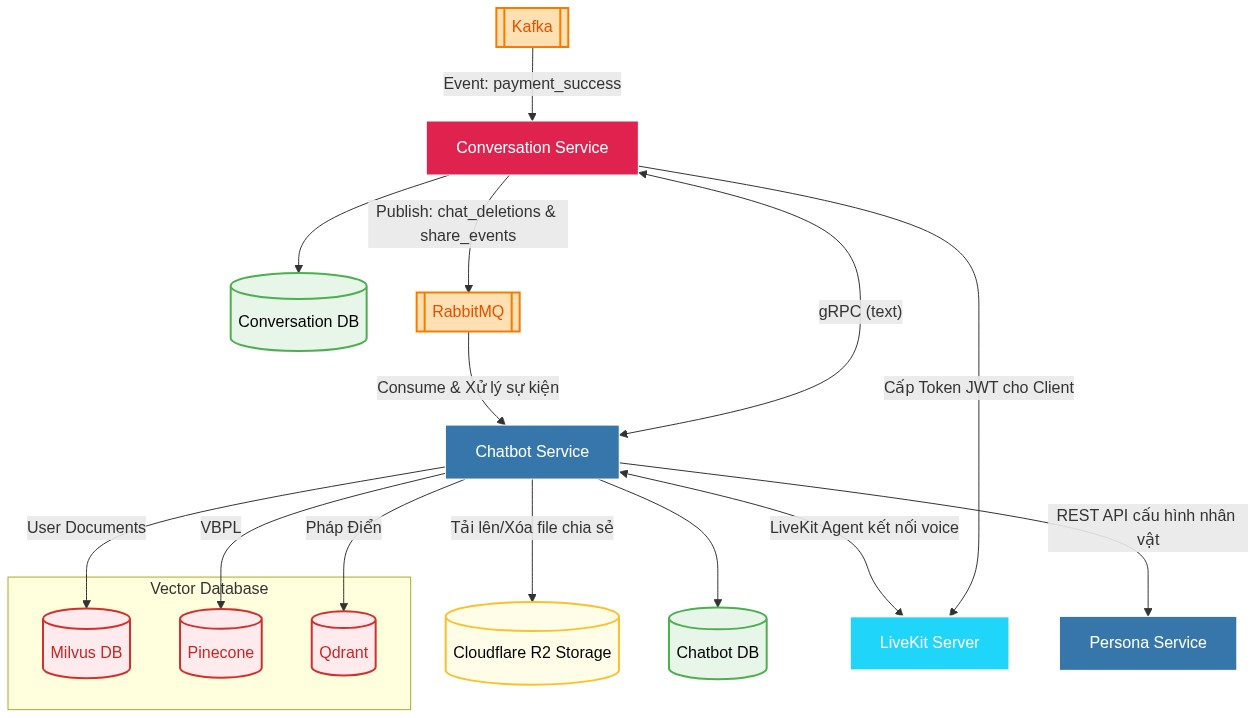
\includegraphics[height=0.7\textheight,width=0.9\textwidth,keepaspectratio]{pictures/conversation-and-chatbot-overview.png}
\caption{Sơ đồ tổng quan dịch vụ trò chuyện và dịch vụ chatbot}
\end{figure}

\note{
Sơ đồ mối quan hệ giữa Dịch vụ trò chuyện (NestJS) và Dịch vụ chatbot (Python).
Dịch vụ trò chuyện chịu trách nhiệm quản lý
trò chuyện của người dùng, lưu trữ lịch sử chat, quản lý thư mục, chia sẻ trò chuyện. Khi có tin nhắn mới, dịch vụ trò chuyện sẽ gửi yêu cầu qua giao thức gRPC hiệu năng cao đến dịch vụ chatbot (Python) để xử lý logic Agentic RAG và trả về câu trả lời dưới dạng stream.
}
\end{frame}


% % \begin{frame}{Kiến trúc tích hợp đàm thoại thời gian thực (Voice Agent)}
\begin{figure}[H]
\centering
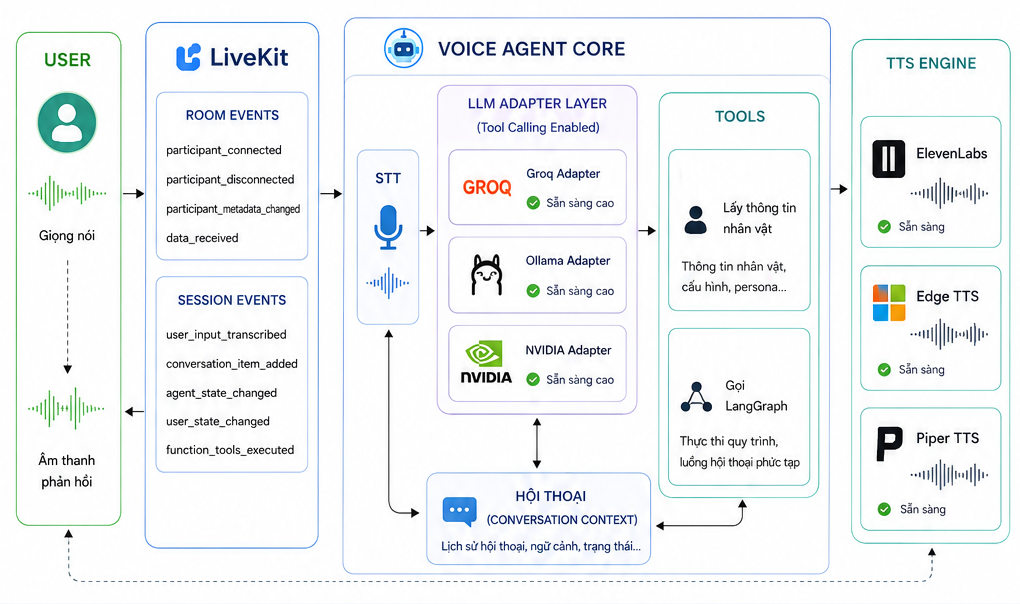
\includegraphics[height=0.7\textheight,width=0.9\textwidth,keepaspectratio]{pictures/voice-livekit-overview.png}
\caption{Sơ đồ tích hợp LiveKit đàm thoại giọng nói}
\end{figure}

\note{
Hệ thống tích hợp máy chủ LiveKit để cung cấp tính năng đàm thoại giọng nói thời gian thực với trợ lý ảo.
Khi người dùng kết nối, Voice Agent hoạt động như một LiveKit Agent, chủ động kết nối và trao đổi âm thanh hai chiều thông qua giao thức WebRTC. Voice Agent tích hợp các mô hình VAD (phát hiện giọng nói), STT (chuyển giọng nói thành văn bản), LLM (suy luận phản hồi) và TTS (chuyển văn bản thành giọng nói) với độ trễ cực thấp.
}
\end{frame}


% \ifdev
% \begin{frame}
\frametitle{}
\maketitle
\end{frame}

\begin{frame}{Cảm ơn}
\centering
\Huge{Thanks for listening!}
\end{frame}

\begin{frame}{Cảm ơn}
\centering
\Huge{Thanks for listening!}
\end{frame}

% \fi

\section{Các công nghệ khác}

\input{contents/Quy_trinh_tu_dong_hoa_CICD_bang_GitHub_Actions}
\begin{frame}{Quản lý Hạ tầng dưới dạng mã}
\begin{figure}[H]
\centering
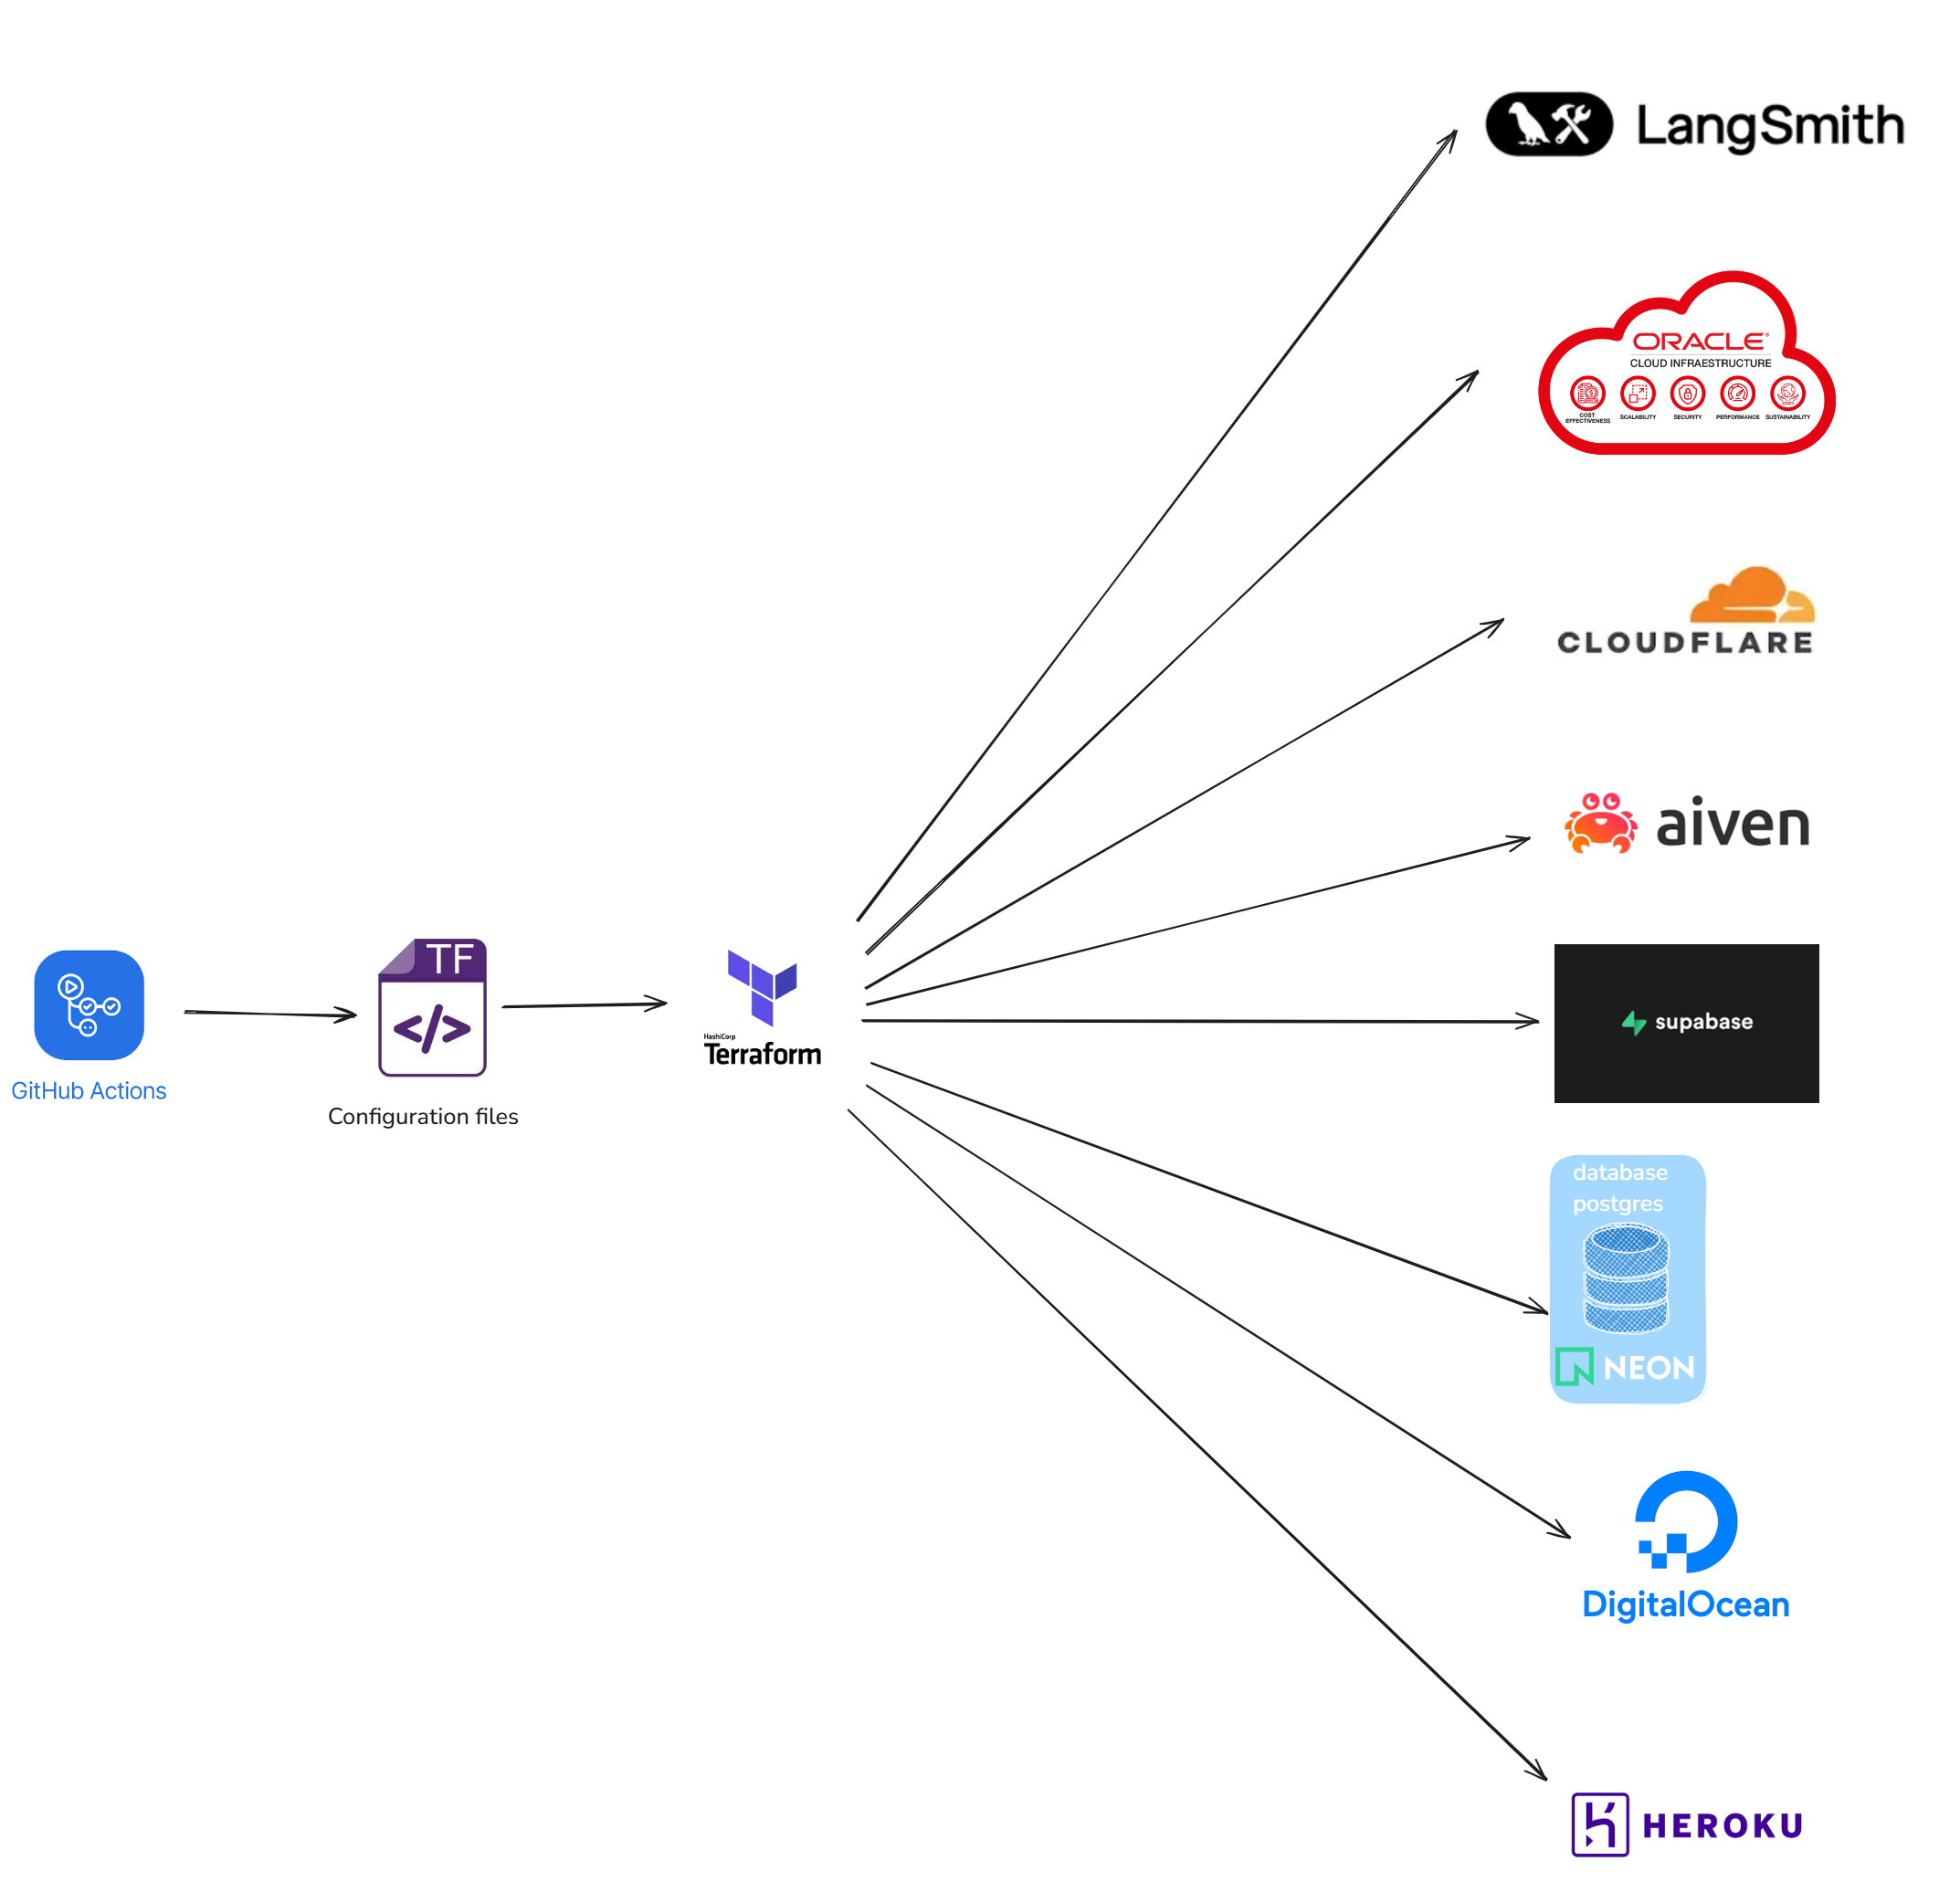
\includegraphics[height=0.7\textheight,width=0.9\textwidth,keepaspectratio]{pictures/infrastructure-as-code-IaC-terraform.excalidraw.png}
\caption{Sơ đồ tổng quan quản lý hạ tầng bằng Terraform trong dự án}
\end{figure}

\note{
Để quản lý hạ tầng một cách nhất quán và tự động, dự án sử dụng Terraform dưới dạng Infrastructure as Code (IaC).
Terraform tự động khởi tạo và cấu hình các tài nguyên bên thứ ba như: Supabase (Auth), LangSmith (giám sát RAG), Cloudflare (DNS và R2 Storage), Neon (PostgreSQL cho các vi dịch vụ), DigitalOcean (Crawl DB) và Heroku (Payment Service). Trạng thái hạ tầng được lưu trữ tập trung trên Terraform Cloud.
}
\end{frame}

\input{contents/Cau_hinh_Kong_API_Gateway_bang_Declarative_Configuration}
\begin{frame}{Kết quả Docker Image trên Docker Hub}
\begin{figure}[H]
\centering
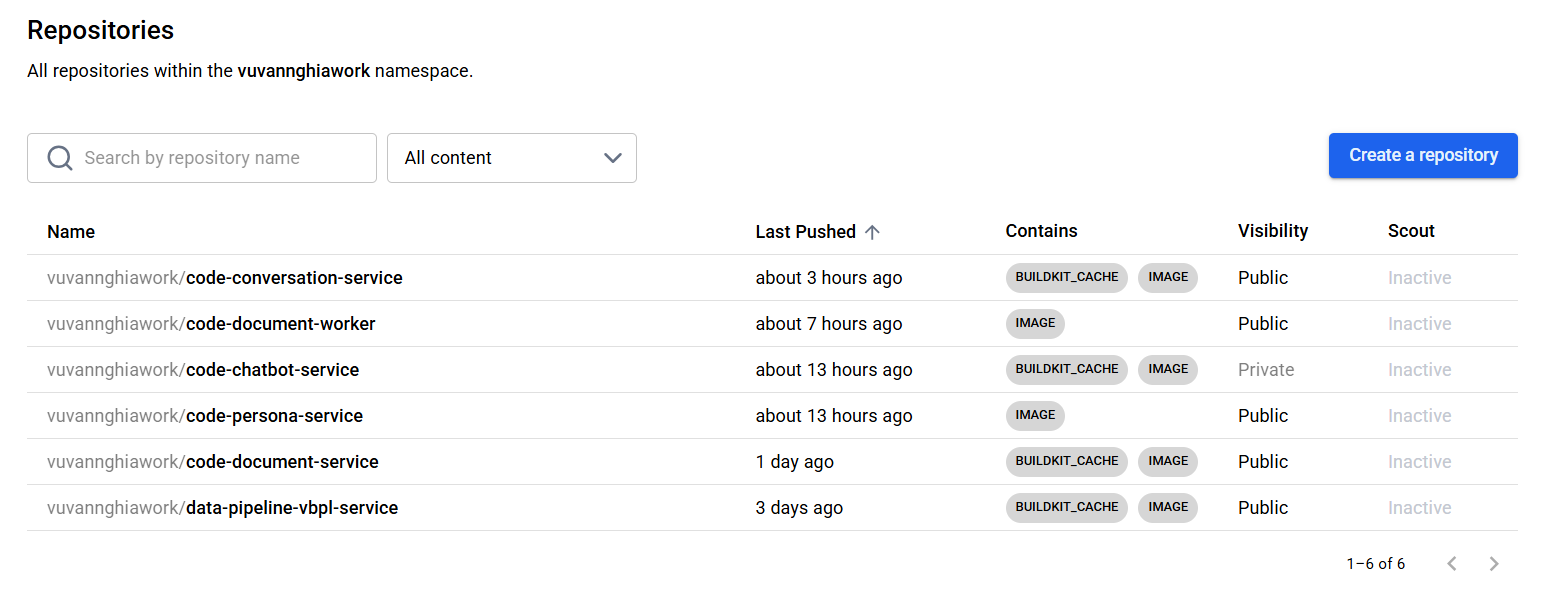
\includegraphics[height=0.55\textheight,width=0.9\textwidth,keepaspectratio]{pictures/docker-hub-web-ui2.png}
\caption{Kết quả Docker Image được push lên Docker Hub}
% \caption{Kết quả giao diện docker}
\end{figure}

\note{
docker
}
\end{frame}

\begin{frame}{Cấu hình tài nguyên Kubernetes trong GitOps Repository}
\begin{figure}[H]
\centering
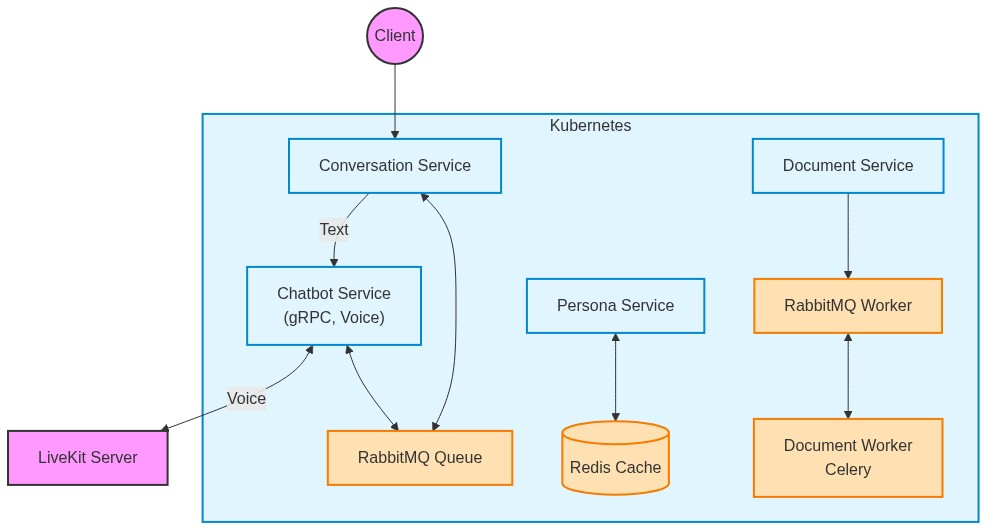
\includegraphics[height=0.55\textheight,width=0.9\textwidth,keepaspectratio]{pictures/Kubernetes.png}
\caption{Cấu hình Kubernetes trong kho lưu trữ GitOps của dự án}
\end{figure}

\note{
Đây là cấu trúc thư mục chứa các file cấu hình Kubernetes (YAML) trong kho lưu trữ GitOps của dự án.
Các dịch vụ nội bộ như RabbitMQ, Redis được chạy trực tiếp trong cụm để giảm độ trễ và được cấu hình dưới dạng ClusterIP để tăng tính bảo mật, ngăn chặn các truy cập trực tiếp từ internet. Các dịch vụ chạy bất đồng bộ như Voice Agent hay Document Worker cũng không công khai service ra bên ngoài.
}
\end{frame}


\begin{frame}{Giao diện quản lý GitOps bằng ArgoCD}
\begin{figure}[H]
\centering
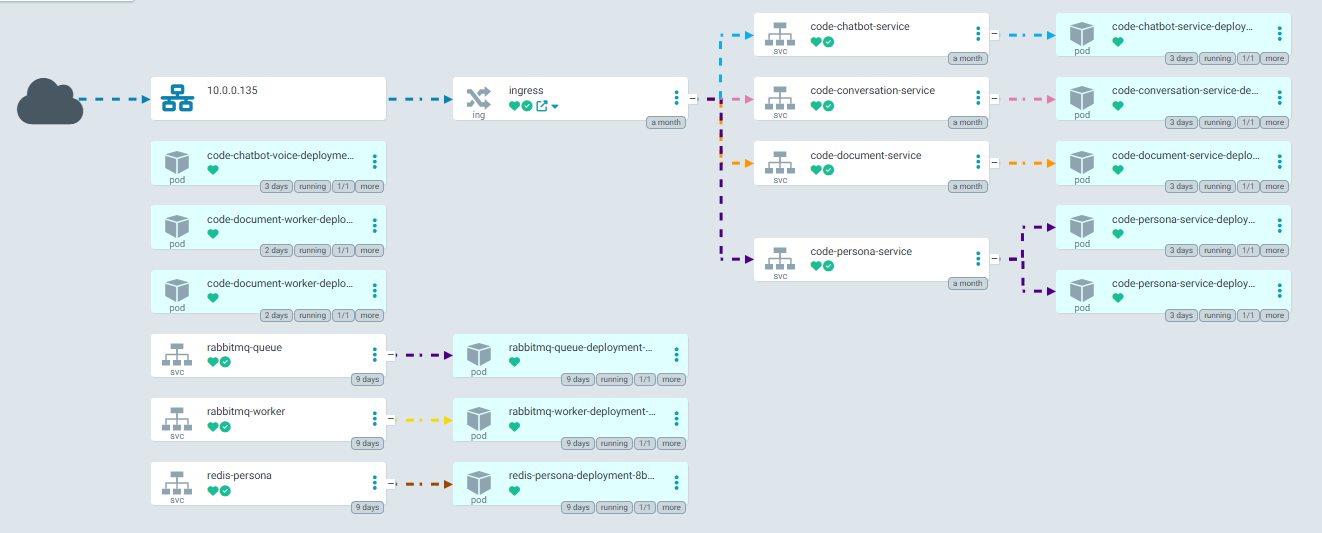
\includegraphics[height=0.55\textheight,width=0.9\textwidth,keepaspectratio]{pictures/argocd-web-ui.png}
\caption{Kết quả giao diện ArgoCD chạy docker trong kubernetes}
\end{figure}

\note{
ArgoCD được triển khai trong cụm Kubernetes để thực hiện quy trình Continuous Delivery (CD) theo mô hình GitOps.
ArgoCD liên tục giám sát kho lưu trữ Git chứa các file cấu hình Kubernetes. Khi phát hiện có sự thay đổi (ví dụ: phiên bản Docker image mới), ArgoCD sẽ tự động đồng bộ (sync) và cập nhật các Pod đang chạy trên Kubernetes thực tế để khớp với cấu hình được khai báo trên Git.
}
\end{frame}


% \begin{titlepage}
\thispagestyle{empty}
% \thisfancypage{
% \setlength{\fboxsep}{3pt}
% \fbox}{}
\begin{center}

{\textbf{\large{ĐẠI HỌC BÁCH KHOA HÀ NỘI}}}\\
{\textbf{\large{KHOA TOÁN - TIN}}}\\[5cm]

{\textbf{\huge{ĐỒ ÁN TỐT NGHIỆP}}}\\[1cm]
{\textbf{\Large{Xây dựng ứng dụng hỗ trợ tư vấn pháp luật \\ sử dụng công nghệ trí tuệ nhân tạo}}\\[1cm]

{\textbf{\large{VŨ VĂN NGHĨA}}}\\
{\large{Email: nghia.vv206205@sis.hust.edu.vn}}\\
{\large{Mã sinh viên: 20206205}}\\[0.5cm]

% {\textbf{\large{Chương trình đào tạo: Công nghệ thông tin Việt-Nhật}}}\\
{\textbf{\large{Chuyên ngành Toán - Tin}}}\\

\vspace{4cm}
% Please add the following required packages to your document preamble:
% \usepackage{graphicx}
\begin{table}[H]
\centering
\resizebox{\textwidth}{!}{%
\begin{tabular}{ll}
\multicolumn{1}{c}{\textbf{Giảng viên hướng dẫn:}} & TS. Trần Anh Tú \hspace{0.5cm} \underline{\hspace{3cm}} \\[0.5cm]
& \multicolumn{1}{r}{Chữ kí GVHD} \\[4cm]
% \textbf{Khoa:} & Kỹ thuật máy tính \\[0.5cm]
% \textbf{Trường:} & Công nghệ Thông tin và Truyền thông \\[4cm]
\multicolumn{2}{c}{\textbf{HÀ NỘI, 06/2026}}
\end{tabular}%
}
\end{table}}
\end{center}

\end{titlepage}

\begin{titlepage}
\thispagestyle{empty}
% \thisfancypage{
% \setlength{\fboxsep}{3pt}
% \fbox}{}
\begin{center}

{\textbf{\large{ĐẠI HỌC BÁCH KHOA HÀ NỘI}}}\\
{\textbf{\large{KHOA TOÁN - TIN}}}\\[5cm]

{\textbf{\huge{ĐỒ ÁN TỐT NGHIỆP}}}\\[1cm]
{\textbf{\Large{Xây dựng ứng dụng hỗ trợ tư vấn pháp luật \\ sử dụng công nghệ trí tuệ nhân tạo}}\\[1cm]

{\textbf{\large{VŨ VĂN NGHĨA}}}\\
{\large{Email: nghia.vv206205@sis.hust.edu.vn}}\\
{\large{Mã sinh viên: 20206205}}\\[0.5cm]

% {\textbf{\large{Chương trình đào tạo: Công nghệ thông tin Việt-Nhật}}}\\
{\textbf{\large{Chuyên ngành Toán - Tin}}}\\

\vspace{4cm}
% Please add the following required packages to your document preamble:
% \usepackage{graphicx}
\begin{table}[H]
\centering
\resizebox{\textwidth}{!}{%
\begin{tabular}{ll}
\multicolumn{1}{c}{\textbf{Giảng viên hướng dẫn:}} & TS. Trần Anh Tú \hspace{0.5cm} \underline{\hspace{3cm}} \\[0.5cm]
& \multicolumn{1}{r}{Chữ kí GVHD} \\[4cm]
% \textbf{Khoa:} & Kỹ thuật máy tính \\[0.5cm]
% \textbf{Trường:} & Công nghệ Thông tin và Truyền thông \\[4cm]
\multicolumn{2}{c}{\textbf{HÀ NỘI, 06/2026}}
\end{tabular}%
}
\end{table}}
\end{center}

\end{titlepage}

\newpage

\vspace*{\fill}
\begin{center}
% Trang này chỉ để trống!
\thispagestyle{empty}
\end{center}
\vspace*{\fill}

\newpage

% \restoregeometry

% \newpage

\newpage
\thispagestyle{empty}

% 1. BẮT ĐẦU CÔ LẬP: Mọi thiết lập font chữ trong này sẽ không ảnh hưởng trang khác
\begingroup

% Nếu bạn cần đổi lề riêng cho trang này, hãy bỏ comment dòng dưới:
% \newgeometry{left=2.2cm,right=2.8cm,top=2cm,bottom=2cm}
% \pagenumbering{roman}
% \setcounter{page}{1}
% \thisfancypage{
% 	\setlength{\fboxsep}{0.5cm}
% 	\fbox}{}

\begin{tikzpicture}[remember picture, overlay]
\path ($(current page text area.north east)+(0.5cm, 0.5cm)$) coordinate (A)
($(current page text area.north west)+(-0.5cm, 0.5cm)$) coordinate (B)
($(current page text area.south west)+(-0.5cm, -0.5cm)$) coordinate (C)
($(current page text area.south east)+(0.5cm, -0.5cm)$) coordinate (D);
\draw[black!40!black, line width=3pt]
(A)--(B)--(C)--(D)--cycle;
\draw[black!10!black, line width=0.5pt]
($(A)+(-0.1cm, -0.1cm)$)--($(B)+(0.1cm, -0.1cm)$)--($(C)+(0.1cm, 0.1cm)$)--($(D)+(-0.1cm, 0.1cm)$)--cycle;
\end{tikzpicture}

\fontsize{13pt}{16pt}\selectfont
\bigbreak
\begin{center}
{\bfseries NHẬN XÉT CỦA GIẢNG VIÊN HƯỚNG DẪN}

\end{center}
\bigbreak

\fontsize{12pt}{14pt}\selectfont

\begin{enumerate}

\item [{\bfseries 1.}]{\bfseries Mục đích và nội dung của đồ án}

\begin{enumerate}
\item Phân tích thiết kế hệ thống chatbot tư vấn pháp luật với dữ liệu thực tế
\item Tìm hiểu và lựa chọn công nghệ xây dựng chatbot phù hợp với bài toán đặt ra
\item Triển khai xây dựng và lập trình hệ thống
\end{enumerate}

\item [{\bfseries 2.}] {\bfseries Kết quả đạt được}

\begin{enumerate}
\item Tìm hiểu và tích hợp nhiều công nghệ có tính cập nhật và độ khó cao trong Đồ án
\item Triển khai data pipeline, thu thập, xử lý và lưu trữ dữ liệu văn bản pháp luật
\item Triển khai xây dựng và lập trình hệ thống có chức năng đúng yêu cầu đặt ra
\end{enumerate}

\item [{\bfseries 3.}]{\bfseries Ý thức làm việc của sinh viên}

\begin{enumerate}
\item Sinh viên chủ động, tích cực trong việc tìm hiểu các công nghệ mới để đưa vào đồ án theo định hướng
\item Sinh viên thực hiện nội dung đúng tiến độ và chủ động báo cáo, xin góp ý hoàn thiện.
\item Sinh viên có ý thức luôn cải tiến, hoàn thiện sản phẩm
\end{enumerate}
\end{enumerate}
\hspace{0.4\textwidth}
\begin{minipage}{0.5\textwidth}
\noindent\begin{center}
\textit{Hà Nội, ngày \dots tháng \dots năm \dots} \\

Giảng viên hướng dẫn \\
\textit{(Ký và ghi rõ họ tên)} \\
\vspace{2cm}
% \textbf{TS. Trần Anh Tú}

\end{center}
\end{minipage}

% 2. KẾT THÚC CÔ LẬP: Trả lại font chữ ban đầu
\endgroup

\newpage
% 3. TRẢ LẠI LỀ GỐC: Nếu ở trên bạn dùng \newgeometry, thì bắt buộc phải bỏ comment dòng dưới
% \restoregeometry
% \restoregeometry

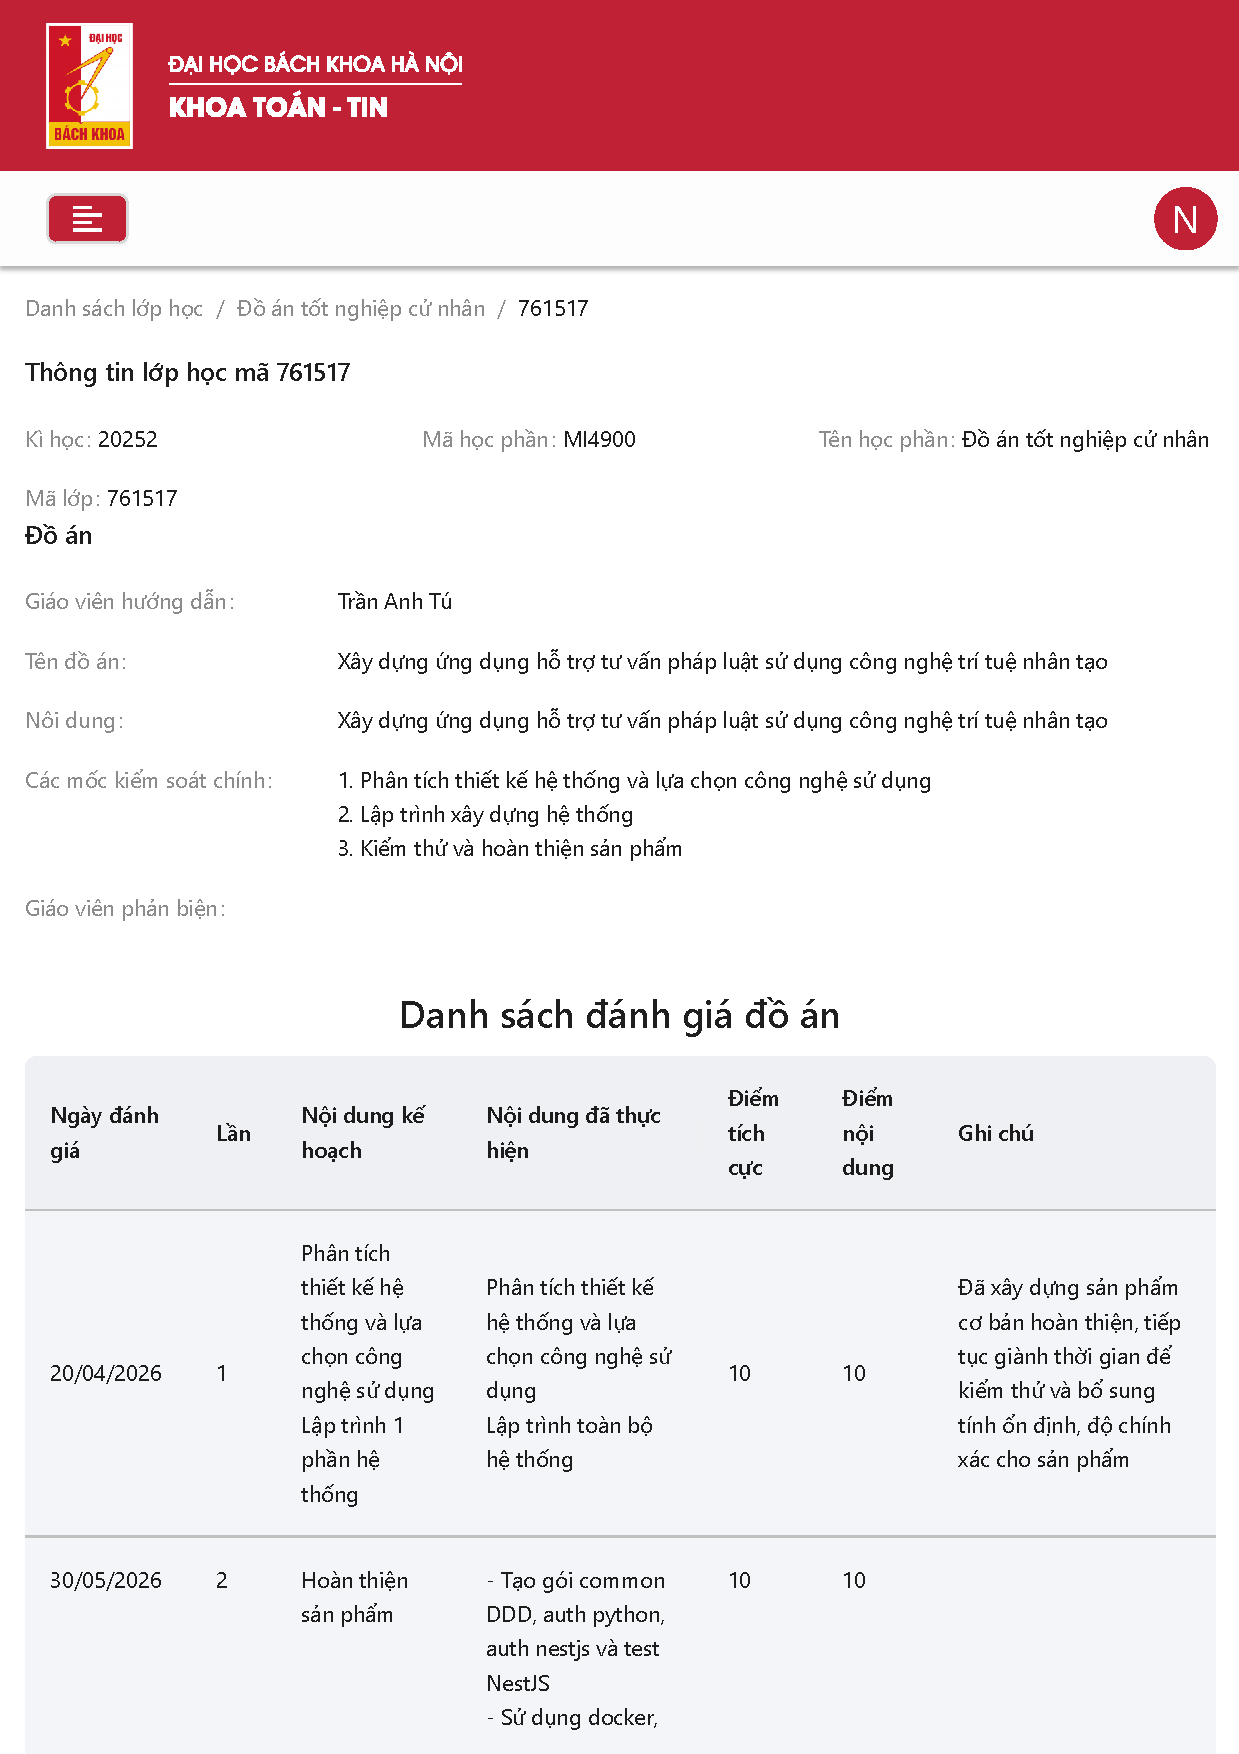
\includepdf[pages=-]{contents/0/bao_cao/danh_gia2.pdf}
{\centering \section*{Lời cảm ơn}}

Qua thời gian học tập và rèn luyện tại
\textit{Đại học Bách khoa Hà Nội},
đến nay em đã hoàn thành đồ án tốt nghiệp.
Trong thời gian học tập để có được kết quả hiện tại
em xin chân thành cảm ơn tới các thầy cô giảng viên trong \textit{Khoa Toán Tin}
đã giảng dạy, quan tâm và tạo điều kiện thuận lợi để em học tập rèn luyện trong suốt thời gian qua,
giúp em trang bị những kiến thức, kỹ năng cần thiết
để em có thể hoàn thành tốt nhất báo cáo này
với
đề tài:
\textit{Xây dựng ứng dụng hỗ trợ tư vấn pháp luật sử dụng công nghệ trí tuệ nhân tạo}.

Đồng thời, em xin gửi lời cảm ơn chân thành và sâu sắc đến \textit{Thầy TS. Trần Anh Tú},
người thầy đã tận tình hỗ trợ,
giúp đỡ và hướng dẫn em suốt thời gian thực hiện đồ án.
Những kiến thức và kinh nghiệm mà em đã tiếp thu được trong quá trình này
sẽ đóng góp quan trọng vào sự phát triển và thành công của em trong tương lai.
Em xin gửi lời chúc sức khỏe tốt nhất đến thầy,
hy vọng thầy luôn dồi dào sức khỏe, đam mê và nhiệt huyết trong công việc giảng dạy.

Em cũng xin gửi lời cảm ơn tới bố mẹ
đã dành nhiều thời gian chăm lo, động viên
và giúp đỡ em để em đạt được thành công trong học tập.

Mặc dù đã cố gắng nỗ lực học hỏi để hoàn thành đồ án,
nhưng thời gian thực hiện đồ án có hạn,
kiến thức của em còn hạn chế.
Do vậy,
không tránh khỏi những thiếu sót,
em rất mong nhận được những ý kiến đóng góp quý báu của thầy cô
để em có thể cải thiện một cách tốt nhất.

\vspace{0.5cm} \emph{Em xin chân thành cảm ơn!}

%%%%%%%%%%%%%%%%%%%%%%%%%%%%%%%%%%%%%%%%%%%%%%%%%%%%%%%
%%%%%%%%%%%%%%%%%%%%%%%%%%%%%%%%%%%%%%%%%%%%%%%%%%%%%%%
%%%%%%%%%%%%%%%%%%%%%%%%%%%%%%%%%%%%%%%%%%%%%%%%%%%%%%%

{\centering \section*{Tóm tắt nội dung đồ án}}

% {
% \color{RedHUST}

% Tóm tắt nội dung của đồ án tốt nghiệp trong khoảng tối đa 300 chữ.
% Phần tóm tắt cần nêu được các ý:
% vấn đề cần thực hiện;
% phương pháp thực hiện;
% công cụ sử dụng (phần mềm, phần cứng…);
% kết quả của đồ án có phù hợp với các vấn đề đã đặt ra hay không;
% tính thực tế của đồ án,
% định hướng phát triển mở rộng của đồ án (nếu có);
% các kiến thức và kỹ năng mà sinh viên đã đạt được.

% }

Đồ án
được thực hiện nhằm giải quyết nhu cầu tra cứu
và giải đáp thông tin pháp luật Việt Nam
(bao gồm Văn bản pháp luật và Pháp Điển) một cách chính xác, nhanh chóng và tự động hóa.

Để tối ưu năng lực giải đáp,
đồ án triển khai hệ thống
Agentic RAG nâng cao sử dụng LangGraph.

Về mặt kiến trúc, hệ thống được thiết kế theo kiến trúc vi dịch vụ (Microservice Architecture),
ứng dụng phương pháp Thiết kế hướng miền (Domain-Driven Design - DDD)
và các dịch vụ được điều phối qua Kong API Gateway.

Để đảm bảo tính ổn định,
hiệu năng cao,
tận dụng điểm mạnh tài nguyên,
thế mạnh framework ngôn ngữ lập trình
và khả năng mở rộng,
các dịch vụ giao tiếp đa dạng từ gRPC cho trò chuyện trực tiếp,
giao tiếp bất đồng bộ giữa các dịch vụ NestJS và Python
được xử lý thông qua RabbitMQ.
Luồng nghiệp vụ
quy trình thanh toán thuê bao VIP
qua các cổng nội địa (VNPay, MoMo, ZaloPay, SePay),
được đồng bộ
sự kiện
bằng nền tảng Kafka.
Toàn bộ vòng đời ứng dụng
được tự động hóa thông qua
CI/CD trên GitHub Actions,
đóng gói bằng Docker và triển khai vận hành trên
cụm Kubernetes thông qua ArgoCD.

Đồ án đã vận hành thành công một trợ lý pháp luật,
đưa ra các tư vấn pháp lý với các bước suy luận logic
và trích dẫn nguồn văn bản rõ ràng.
Bên cạnh đó,
ứng dụng còn mang đến trải nghiệm đàm thoại
thời gian thực bằng cách tích hợp LiveKit
cùng các mô hình xử lý giọng nói tiên tiến như Whisper (Speech-to-Text), Edge, Piper và ElevenLabs (Text-to-Speech).

\begin{flushright}
\begin{tabular}{c}
% Hà Nội, \today \\
\textit{Hà Nội, ngày \dots tháng \dots năm \dots} \\
Sinh viên thực hiện \\
\textit{(Ký và ghi rõ họ tên)} \\
% Nghĩa \\
% Vũ Văn Nghĩa
\end{tabular}
\end{flushright}

\newpage

\renewcommand{\contentsname}{MỤC LỤC} % ĐẶT TÊN TIÊU ĐỀ MỤC LỤC
\tableofcontents

\newpage

% DANH MỤC KÝ HIỆU

\newpage
\phantomsection
{\centering \section*{DANH MỤC KÝ HIỆU}} % Đặt tên tiêu đề
\addcontentsline{toc}{section}{DANH MỤC KÝ HIỆU} % Thêm vào mục lục

\begin{table}[ht]
\centering
\small
\begin{tabular}{|c|p{2.1cm}|p{4.3cm}|p{5.4cm}|}
\hline
\textbf{STT} & \textbf{Từ viết tắt} & \textbf{Từ viết đầy đủ} & \textbf{Mô tả} \\ \hline
1 & 2FA & Two-Factor Authentication & Xác thực hai yếu tố \\ \hline
2 & AAL1 / AAL2 & \makecell[l]{Authenticator Assurance \\ Level 1 / 2} & Mức độ đảm bảo xác thực 1 / 2 \\ \hline
3 & AI & Artificial Intelligence & Trí tuệ nhân tạo \\ \hline
4 & API & \makecell[l]{Application Programming \\ Interface} & Giao diện lập trình ứng dụng \\ \hline
5 & CD & \makecell[l]{Continuous \\ Delivery / Deployment} & Chuyển giao/Triển khai liên tục \\ \hline
6 & CI & Continuous Integration & Tích hợp liên tục \\ \hline
7 & CLI & Command Line Interface & Giao diện dòng lệnh \\ \hline
8 & CSDL & Cơ sở dữ liệu & Cơ sở dữ liệu \\ \hline
9 & DB & Database & Cơ sở dữ liệu \\ \hline
10 & DDD & Domain Driven Design & Thiết kế hướng miền \\ \hline
11 & DLQ & Dead Letter Queue & Hàng đợi thư lỗi \\ \hline
12 & DNS & Domain Name System & Hệ thống phân giải tên miền \\ \hline
13 & HTML & Hyper Text Markup Language & Ngôn ngữ Đánh dấu Siêu văn bản \\ \hline
14 & IPN & Instant Payment Notification & Thông báo thanh toán tức thì \\ \hline
15 & IaC & Infrastructure as Code & Cơ sở hạ tầng dưới dạng mã \\ \hline
16 & JWT & JSON Web Token & Tiêu chuẩn truyền tải thông tin JSON \\ \hline
17 & K8s & Kubernetes & Công cụ quản lý container \\ \hline
18 & LLM & Large Language Model & Mô hình ngôn ngữ lớn \\ \hline
19 & LRU & Least Recently Used & \makecell[l]{Thuật toán loại bỏ dữ liệu \\ ít được sử dụng gần đây nhất} \\ \hline
20 & MFA & Multi-Factor Authentication & Xác thực đa yếu tố \\ \hline
21 & NLP & Natural Language Processing & Xử lý ngôn ngữ tự nhiên \\ \hline
22 & PSC & Payment Service Consumer & Đơn vị sử dụng dịch vụ thanh toán \\ \hline
23 & PSP & Payment Service Provider & Đơn vị cung cấp dịch vụ thanh toán \\ \hline
24 & QR Code & Quick Response Code & Mã phản hồi nhanh \\ \hline
25 & RAG & \makecell[l]{Retrieval Augmented \\ Generation} & Tạo tăng cường truy xuất \\ \hline
26 & RLS & Row-Level Security & Bảo mật cấp hàng \\ \hline
27 & SMTP & Simple Mail Transfer Protocol & Giao thức truyền thư đơn giản \\ \hline
28 & SQL & Structured Query Language & Ngôn ngữ truy vấn cấu trúc \\ \hline
29 & SSE & Server-sent events & Sự kiện máy chủ gửi \\ \hline
30 & STT & Speech to Text & Chuyển giọng nói thành văn bản \\ \hline
31 & TOTP & \makecell[l]{Time-based \\ One-Time Password} & \makecell[l]{Mật khẩu dùng một lần \\ dựa trên thời gian} \\ \hline
32 & TTL & Time To Live & Thời gian tồn tại \\ \hline
33 & TTS & Text to Speech & Chuyển văn bản thành giọng nói \\ \hline
34 & UI & User Interface & Giao diện người dùng \\ \hline
35 & UML & Unified Modeling Language & Ngôn ngữ mô hình hóa thống nhất \\ \hline
36 & URL & Uniform Resource Locator & Trình định vị tài nguyên đồng nhất \\ \hline
37 & UUID & Universally Unique Identifier & Mã định danh duy nhất toàn cầu \\ \hline
38 & VBPL & Văn bản pháp luật & Văn bản pháp luật \\ \hline
39 & VIP & Very Important Person & Người rất quan trọng \\ \hline
40 & VPS & Virtual Private Server & Máy chủ riêng ảo \\ \hline
41 & gRPC & gRPC Remote Procedure Call & \makecell[l]{Framework Gọi thủ tục từ xa \\ do Google phát triển} \\ \hline
\end{tabular}
\end{table}

\newpage

% DANH MỤC HÌNH VẼ

\newpage
\phantomsection

\renewcommand{\listfigurename}{DANH MỤC HÌNH VẼ} % ĐẶT TÊN TIÊU ĐỀ
\addcontentsline{toc}{section}{DANH MỤC HÌNH VẼ} % THÊM VÀO MỤC LỤC
\makeatletter
\renewcommand*\l@figure{\@dottedtocline{1}{1.5em}{5.5em}}
\makeatother
{\let\oldnumberline\numberline
\renewcommand{\numberline}[1]{\oldnumberline{Hình~#1}}
\listoffigures}

\newpage

% DANH MỤC BẢNG BIỂU

\newpage
\phantomsection

\renewcommand{\listtablename}{DANH MỤC BẢNG BIỂU}
\makeatletter
\renewcommand{\listoftables}{
\begin{center}
\section*{\listtablename}
\end{center}
\@starttoc{lot}
}
\renewcommand*\l@table{\@dottedtocline{1}{1.5em}{5.5em}}
\makeatother
\addcontentsline{toc}{section}{DANH MỤC BẢNG BIỂU}
{\let\oldnumberline\numberline
\renewcommand{\numberline}[1]{\oldnumberline{Bảng~#1}}
\listoftables}

\newpage

%%%%%%%%%%%%%%%%%%%%%%%%%%%%%%%%%%%%%%%%%%%%%%%%%%%%%%%
% % % % \section{Bài toán nghiệp vụ}

% % % % \begin{frame}{Sự cần thiết}

\begin{itemize}

\item Hệ thống pháp luật rất phức tạp

\item Cá nhân, doanh nghiệp bỏ lỡ cập nhật

\end{itemize}

\begin{figure}[H]
\centering

\includegraphics[width=\linewidth,height=0.55\textheight,keepaspectratio]{pictures/chatbot-tra-cuu-luat-la-gi.jpeg}
\caption[AI hỗ trợ tư vấn pháp luật]{AI hỗ trợ tư vấn pháp luật (Nguồn: \footnotemark)}
\end{figure}
\footnotetext{\url{https://vnptai.io/vi/blog/detail/chatbot-ai-tra-cuu-luat}}

\note{

Hệ thống pháp luật rất phức tạp.

\hrule

Các VBPL có thể thay thế, bổ sung VBPL khác,

hoặc bị hết hiệu lực.

\hrule

Nếu cá nhân, doanh nghiệp bỏ lỡ cập nhật

Và vô tình áp dụng sai luật

\hrule

=> Dẫn đến hậu quả tài chính và rủi ro pháp lý

}

\end{frame}

% hệ thống pháp luật rất phức tạp.

% các văn bản pháp luật có thể thay thế, bổ sung văn bản pháp luật khác

% hoặc bị hết hiệu lực. nếu cá nhân, doanh nghiệp bỏ lỡ cập nhật

% và vô tình áp dụng sai luật. dẫn đến hậu quả tài chính và rủi ro pháp lý


% % % % \begin{frame}{Vai trò và chức năng}
\begin{table}
\centering
\caption{Bảng vai trò và chức năng trong hệ thống} % <-- Lệnh caption được thêm ở đây

% Bây giờ cả hai cột đều có thể dùng 'l' (căn trái) hoặc 'c' (căn giữa)
\begin{tabular}{|l|l|}
\hline
\textbf{Vai trò} & \textbf{Chức năng} \\
\hline

% Dòng 1: Guest
Guest &
\makecell[l]{ % [l] để căn trái các dòng bên trong ô
Giới thiệu, nghe thử giọng nói, xem gói VIP \\
Đăng ký email,
Đăng nhập \textbf{
\textcolor{blue}{G}%
\textcolor{red}{o}%
\textcolor{yellow}{o}%
\textcolor{blue}{g}%
\textcolor{green}{l}%
\textcolor{red}{e}
}
} \\
\hline

% Dòng 2: User
User &
\makecell[l]{
Đăng nhập và quản lý tài khoản, cài đặt \\
Thực hiện trò chuyện, đánh dấu và chia sẻ \\
Mua gói VIP và xem lịch sử
} \\
\hline

% Dòng 3: VIP
VIP &
\makecell[l]{
Suy luận nâng cao\\
Tài liệu cá nhân \\
Sử dụng giọng nói
} \\
\hline

% Dòng 4: Admin
Admin &
\makecell[l]{
Quản lý nhân vật,
gói VIP \\
Báo cáo đường ống dữ liệu
} \\
\hline
\end{tabular}
\end{table}
\end{frame}


% % % % \begin{frame}{Sơ đồ Use Case - Khách vãng lai}
\begin{figure}[H]
\centering
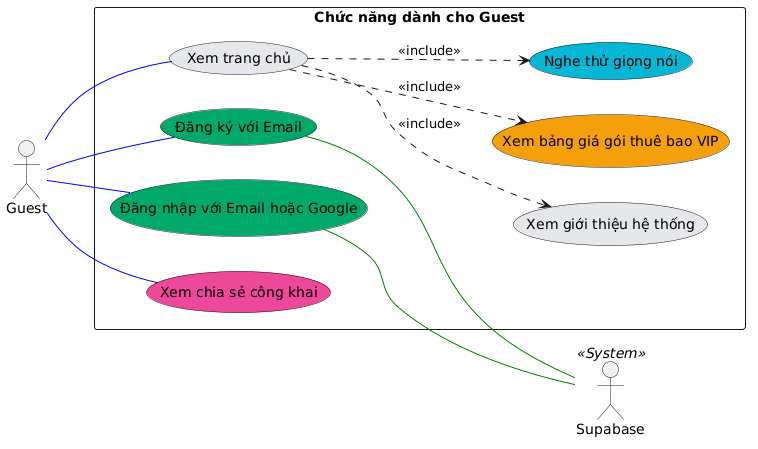
\includegraphics[width=\linewidth,height=0.74\textheight,keepaspectratio]{pictures/UML-UseCase-Guest.png}
\caption{Sơ đồ Use Case chức năng của khách vãng lai}
\end{figure}

\note{

dưới đây là sơ đồ iu cây dành cho người dùng trong hệ thống
\hrule

đầu tiên là khách vãng lai (chưa đăng nhập hệ thống)
\hrule

tiếp theo sơ đồ iu cây dành cho người dùng cơ bản (đã đăng nhập)
\hrule

tiếp theo sơ đồ iu cây dành cho người dùng vip
\hrule

cuối cùng là sơ đồ iu cây dành cho quản trị viên (admin)

}
\end{frame}

% % % % \begin{frame}{Sơ đồ Use Case - Người dùng cơ bản}
\begin{figure}[H]
\centering
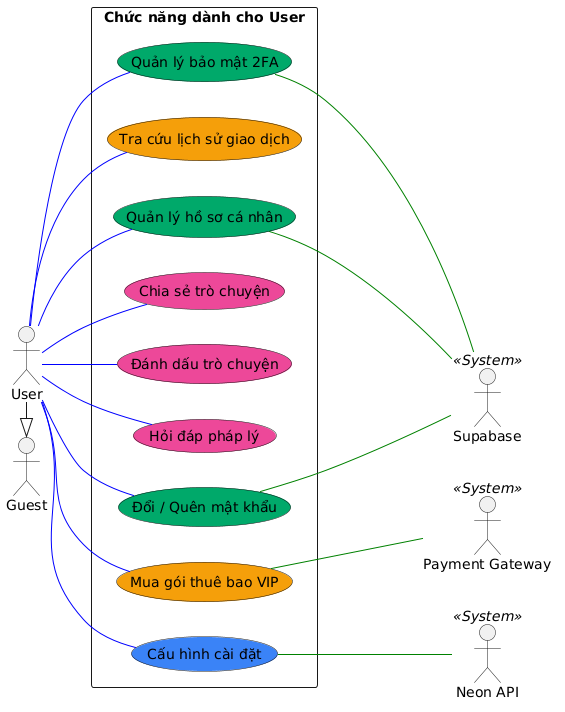
\includegraphics[width=\linewidth,height=0.74\textheight,keepaspectratio]{pictures/UML-UseCase-User.png}
\caption{Sơ đồ Use Case chức năng của người dùng cơ bản}
\end{figure}

\note{

Dưới đây là

Sơ đồ Use Case
chi tiết

dành cho người dùng cơ bản
(đã đăng nhập).

}
\end{frame}

% % % % \begin{frame}{Sơ đồ Use Case - Người dùng VIP}
\begin{figure}[H]
\centering
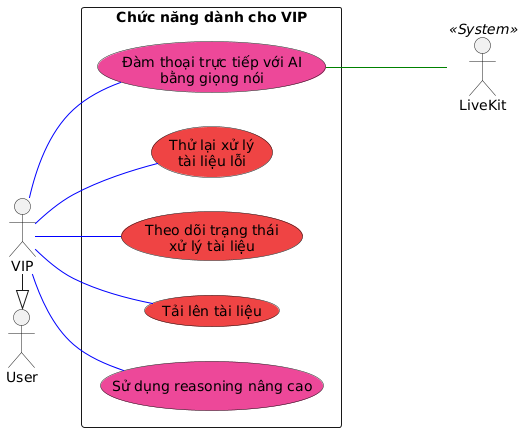
\includegraphics[width=\linewidth,height=0.74\textheight,keepaspectratio]{pictures/UML-UseCase-VIP.png}
\caption{Sơ đồ Use Case chức năng của người dùng VIP}
\end{figure}

\note{

Dưới đây là

Sơ đồ Use Case
chi tiết

dành cho nhóm người dùng VIP.

}
\end{frame}

% % % % \begin{frame}{Sơ đồ Use Case - Quản trị viên}
\begin{figure}[H]
\centering
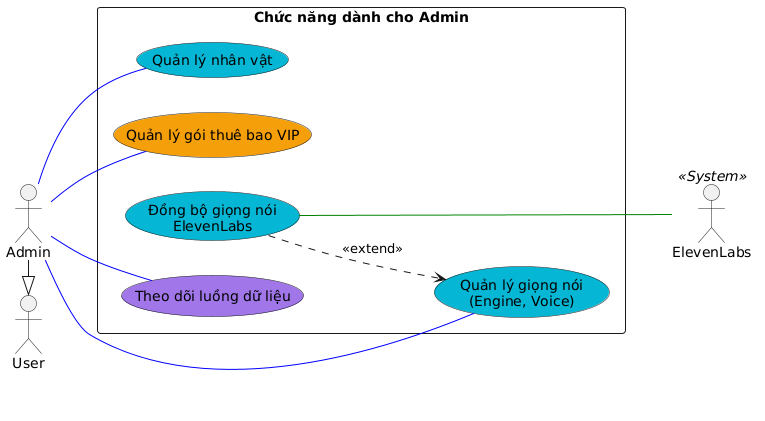
\includegraphics[width=\linewidth,height=0.72\textheight,keepaspectratio]{pictures/UML-UseCase-Admin.png}
\caption{Sơ đồ Use Case chức năng của quản trị viên}
\end{figure}

\note{
Sơ đồ Use Case dành cho quản trị viên (Admin).
Quản trị viên có các quyền hạn cao nhất trong hệ thống bao gồm: quản lý danh sách người dùng, quản lý cấu hình các gói thanh toán VIP, giám sát hệ thống, xem các báo cáo thống kê giao dịch và quản lý các tài liệu pháp luật chung trong CSDL tri thức của hệ thống.
}
\end{frame}


% % % \section{Xây dựng hệ thống AI}
% % % \subsection{Đường ống dữ liệu}

% % % \begin{frame}{Đường ống dữ liệu văn bản pháp luật (VBPL)}
\begin{figure}[H]
\centering
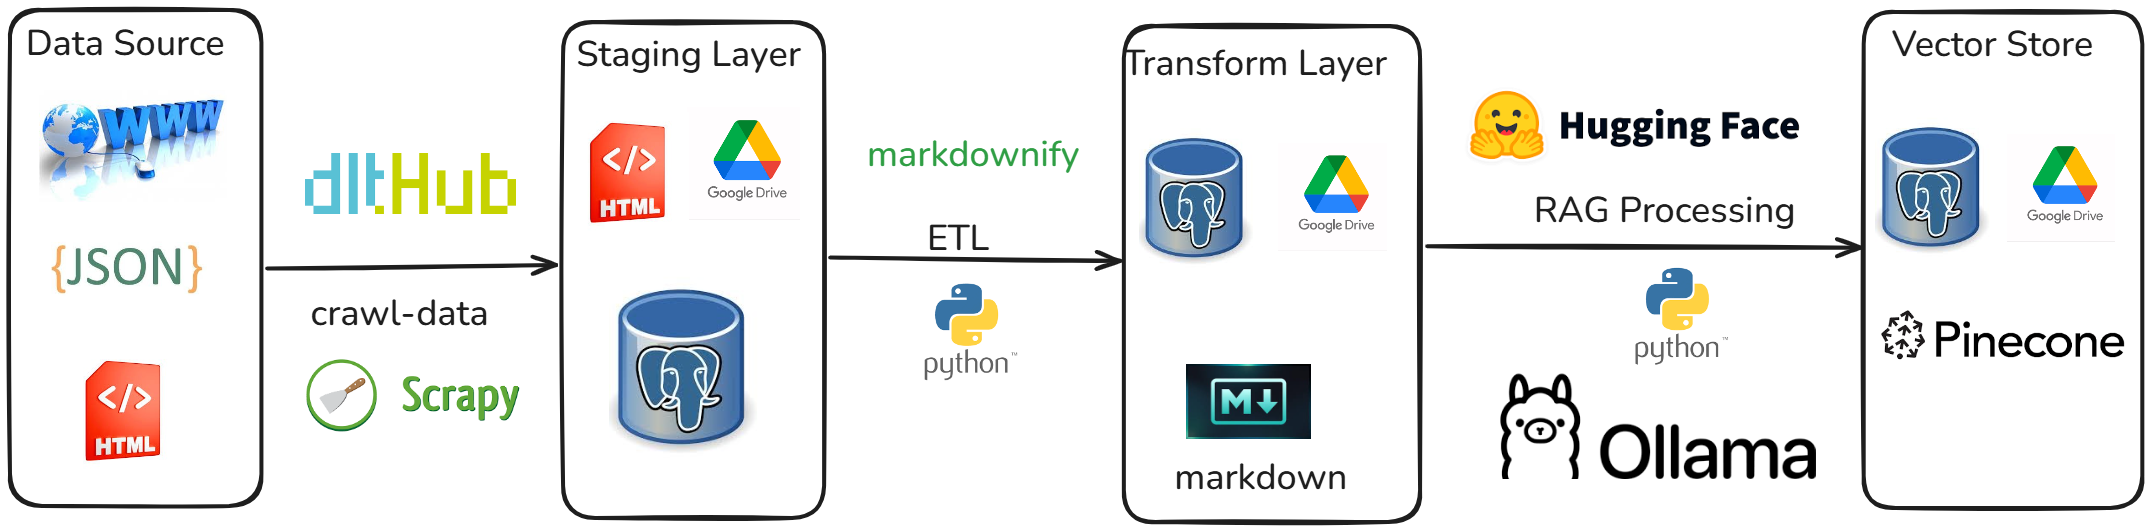
\includegraphics[height=0.55\textheight,width=0.9\textwidth,keepaspectratio]{pictures/Data-Pipeline-VBPL.excalidraw.png}
\caption{Sơ đồ tổng quan luồng dữ liệu văn bản pháp luật mới}
\end{figure}

\note{
Do nguồn dữ liệu Văn bản pháp luật Việt Nam (VBPL) thay đổi cấu trúc trang web và API vào tháng 5/2026, dự án đã xây dựng lại đường ống dữ liệu mới.
Đường ống dữ liệu này tự động hóa quy trình từ thu thập thông tin qua crawler, lưu trữ dữ liệu thô vào PostgreSQL, thực hiện tiền xử lý văn bản pháp luật và cuối cùng là tích hợp vào RAG pipeline để cập nhật CSDL tri thức của trợ lý ảo.
}
\end{frame}

% % % \begin{frame}{Quy trình các bước thu thập dữ liệu văn bản pháp luật}
\begin{figure}[H]
\centering
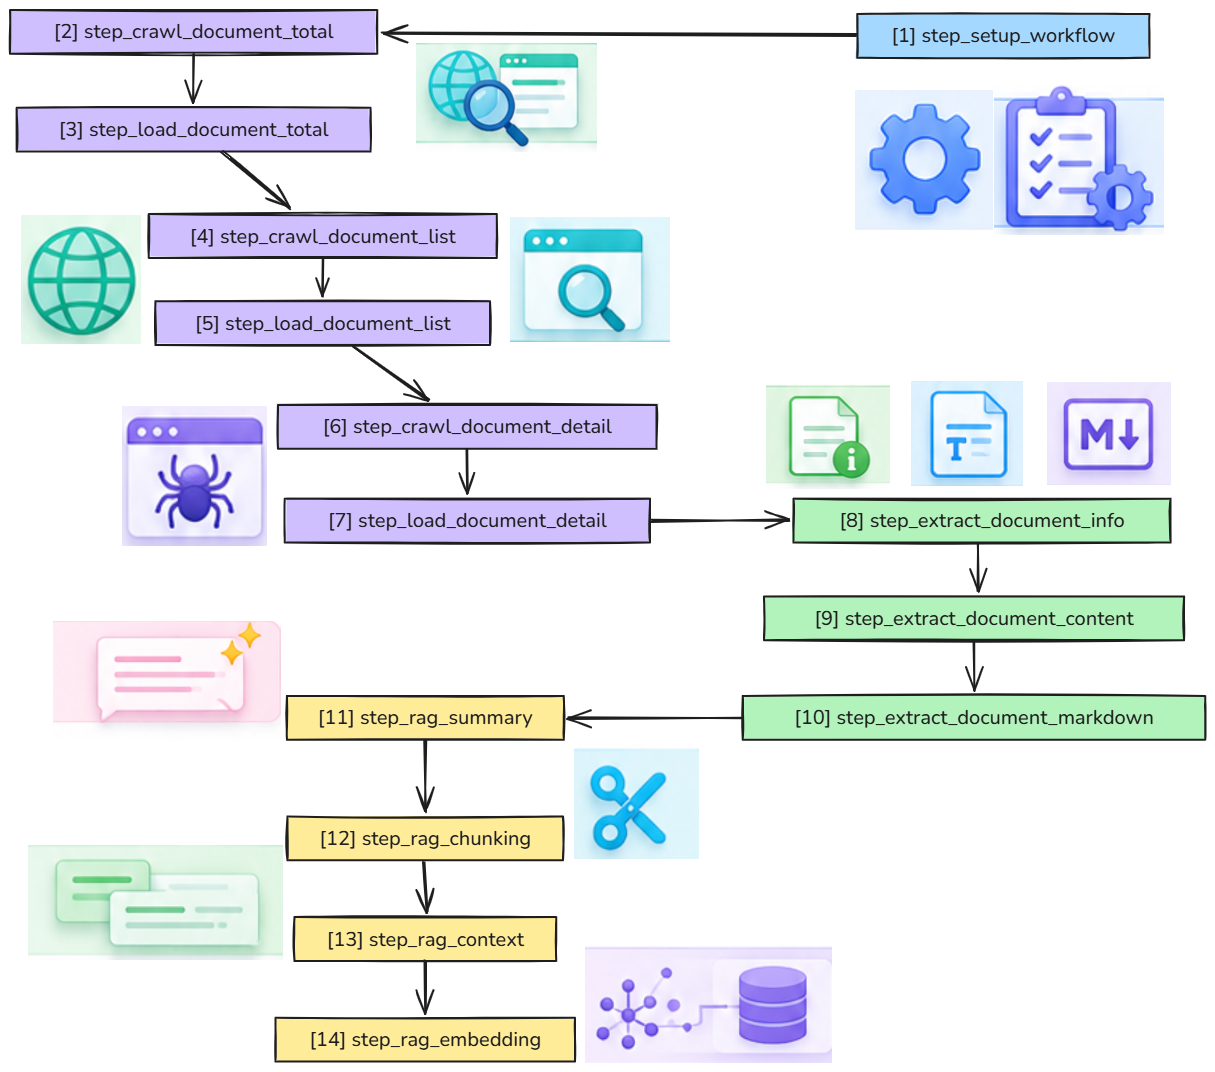
\includegraphics[height=0.55\textheight,width=0.9\textwidth,keepaspectratio]{pictures/step0.excalidraw.png}
\caption{Sơ đồ các bước thực hiện của quy trình cũ}
\end{figure}

\note{
Sơ đồ chi tiết các bước thực hiện trong quy trình cũ của đường ống dữ liệu văn bản pháp luật.
Quy trình được chia thành 3 giai đoạn: Khởi tạo luồng công việc (\texttt{step\_setup\_workflow}), thu thập tổng số lượng tài liệu (\texttt{step\_crawl\_document\_total}), tải nội dung chi tiết và cuối cùng là xử lý định dạng văn bản để chuẩn bị cho việc trích xuất thông tin.
}
\end{frame}

% % % \begin{frame}{Các bước trong đường ống dữ liệu VBPL mới}
\begin{figure}[H]
\centering
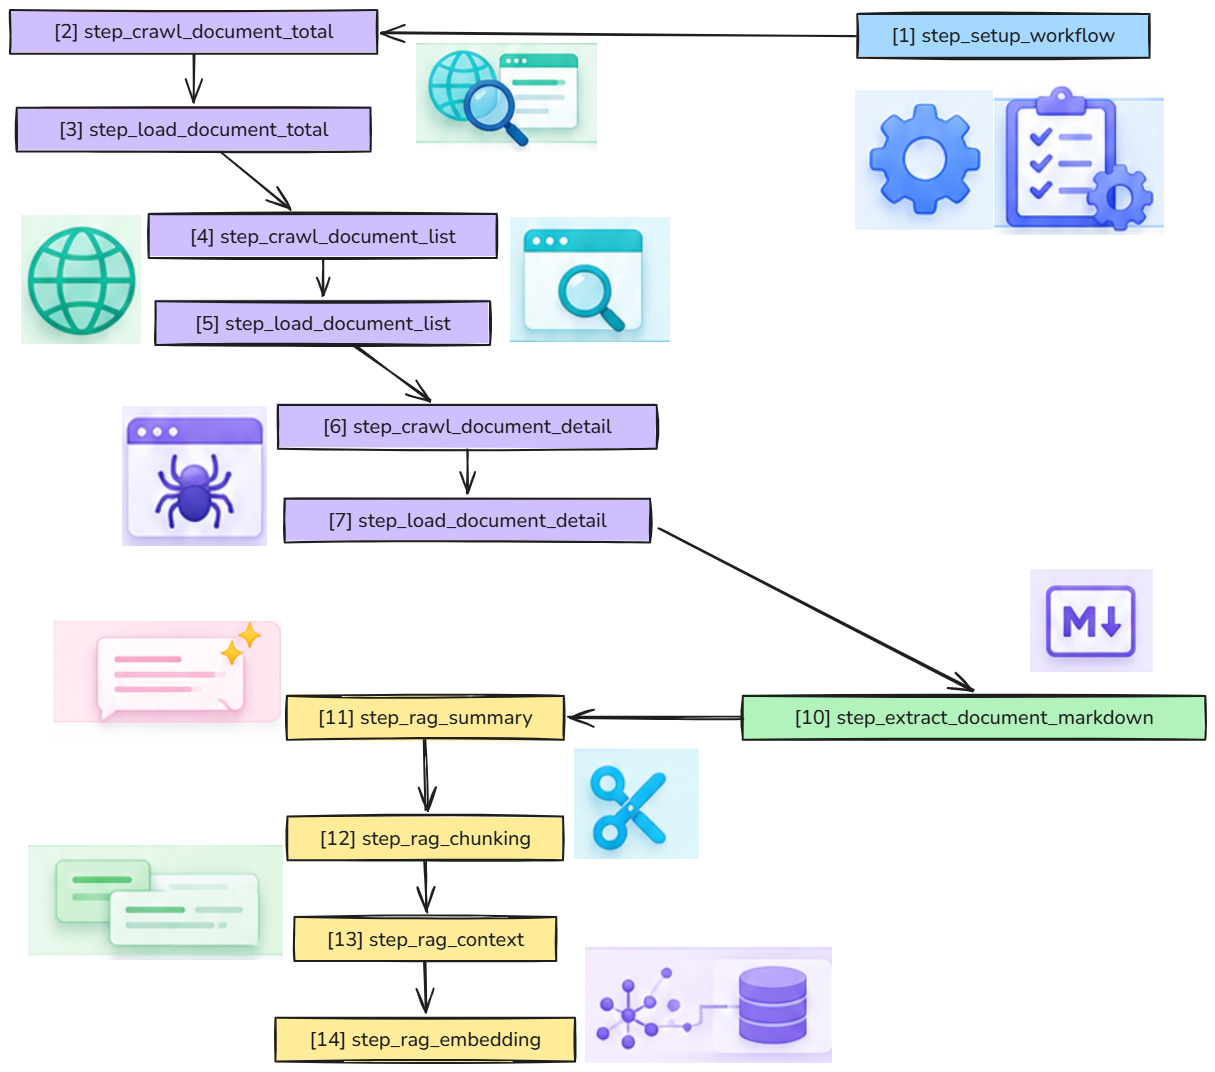
\includegraphics[height=0.7\textheight,width=0.9\textwidth,keepaspectratio]{pictures/step1.excalidraw.png}
\caption{Sơ đồ các bước thực hiện của quy trình mới}
\end{figure}

\note{
do api => bỏ bước

Sơ đồ các bước thực hiện của quy trình mới
}
\end{frame}

% % % \begin{frame}{Đường ống dữ liệu Pháp Điển}
\begin{figure}[H]
\centering
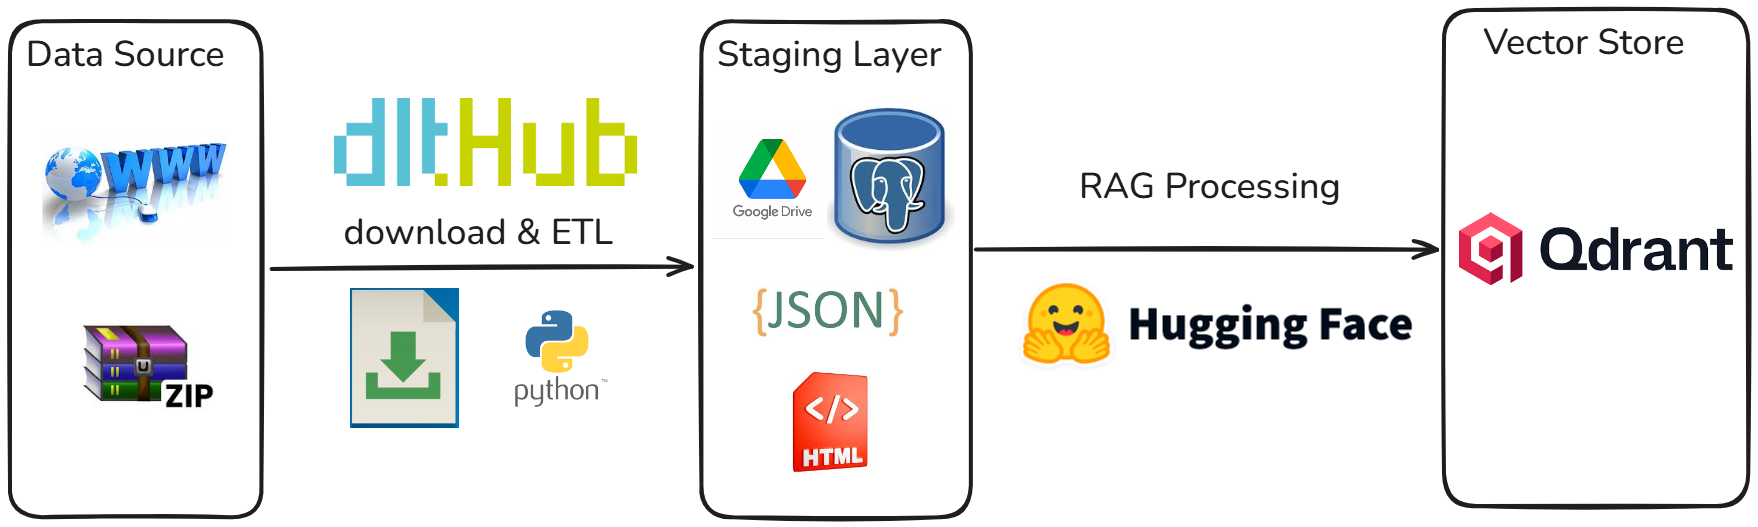
\includegraphics[height=0.55\textheight,width=0.9\textwidth,keepaspectratio]{pictures/Data-Pipeline-PhapDien.excalidraw.png}
\caption{Sơ đồ tổng quan đường ống dữ liệu Pháp Điển}
\end{figure}

\note{
Bên cạnh VBPL, hệ thống còn tích hợp Bộ Pháp Điển Việt Nam. Sơ đồ này mô tả đường ống dữ liệu Pháp Điển.
Dữ liệu Pháp Điển được tải về dưới dạng file nén ZIP từ Cổng thông tin điện tử Pháp Điển, sau đó được giải nén, chuyển đổi cấu trúc cây đề mục sang định dạng JSON, tải lên lưu trữ trên Google Drive và thực hiện vector hóa để lưu vào Vector Database.
}
\end{frame}

% % % \begin{frame}{Các bước trong đường ống dữ liệu Pháp Điển}

\begin{figure}[H]
\centering
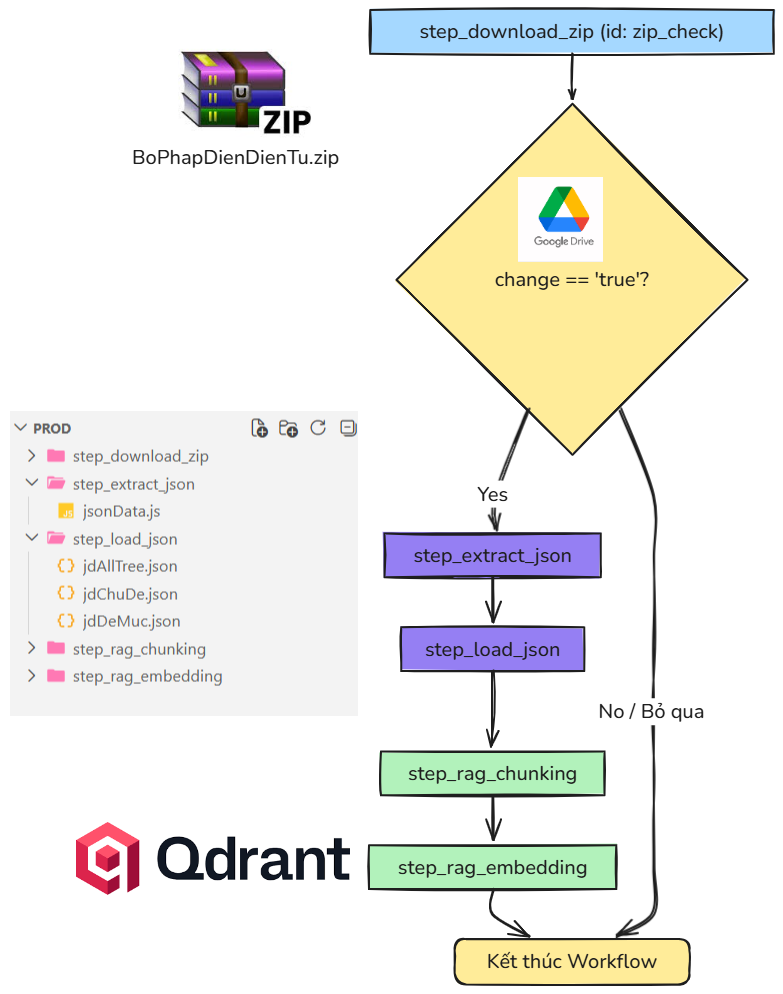
\includegraphics[height=0.7\textheight,width=0.9\textwidth,keepaspectratio]{pictures/step3.excalidraw.png}
\caption{Sơ đồ các bước thực hiện của đường ống dữ liệu Pháp Điển}
\end{figure}

\note{
Sơ đồ mô tả quy trình từng bước của đường ống dữ liệu Pháp Điển.
Quy trình bắt đầu từ việc tải file ZIP tự động (\texttt{step\_download\_zip}), tính toán mã băm MD5 để kiểm tra sự thay đổi dữ liệu so với phiên bản trước, giải nén và trích xuất cấu trúc đề mục ra các file JSON riêng biệt, sau đó chạy các tác vụ phân tích cấu trúc và lưu kết quả vector hóa.
}
\end{frame}


% % % \subsection{Agentic RAG với LangGraph}

% % % \begin{frame}{Kiến trúc Agentic RAG bằng LangGraph}
\begin{figure}[H]
\centering
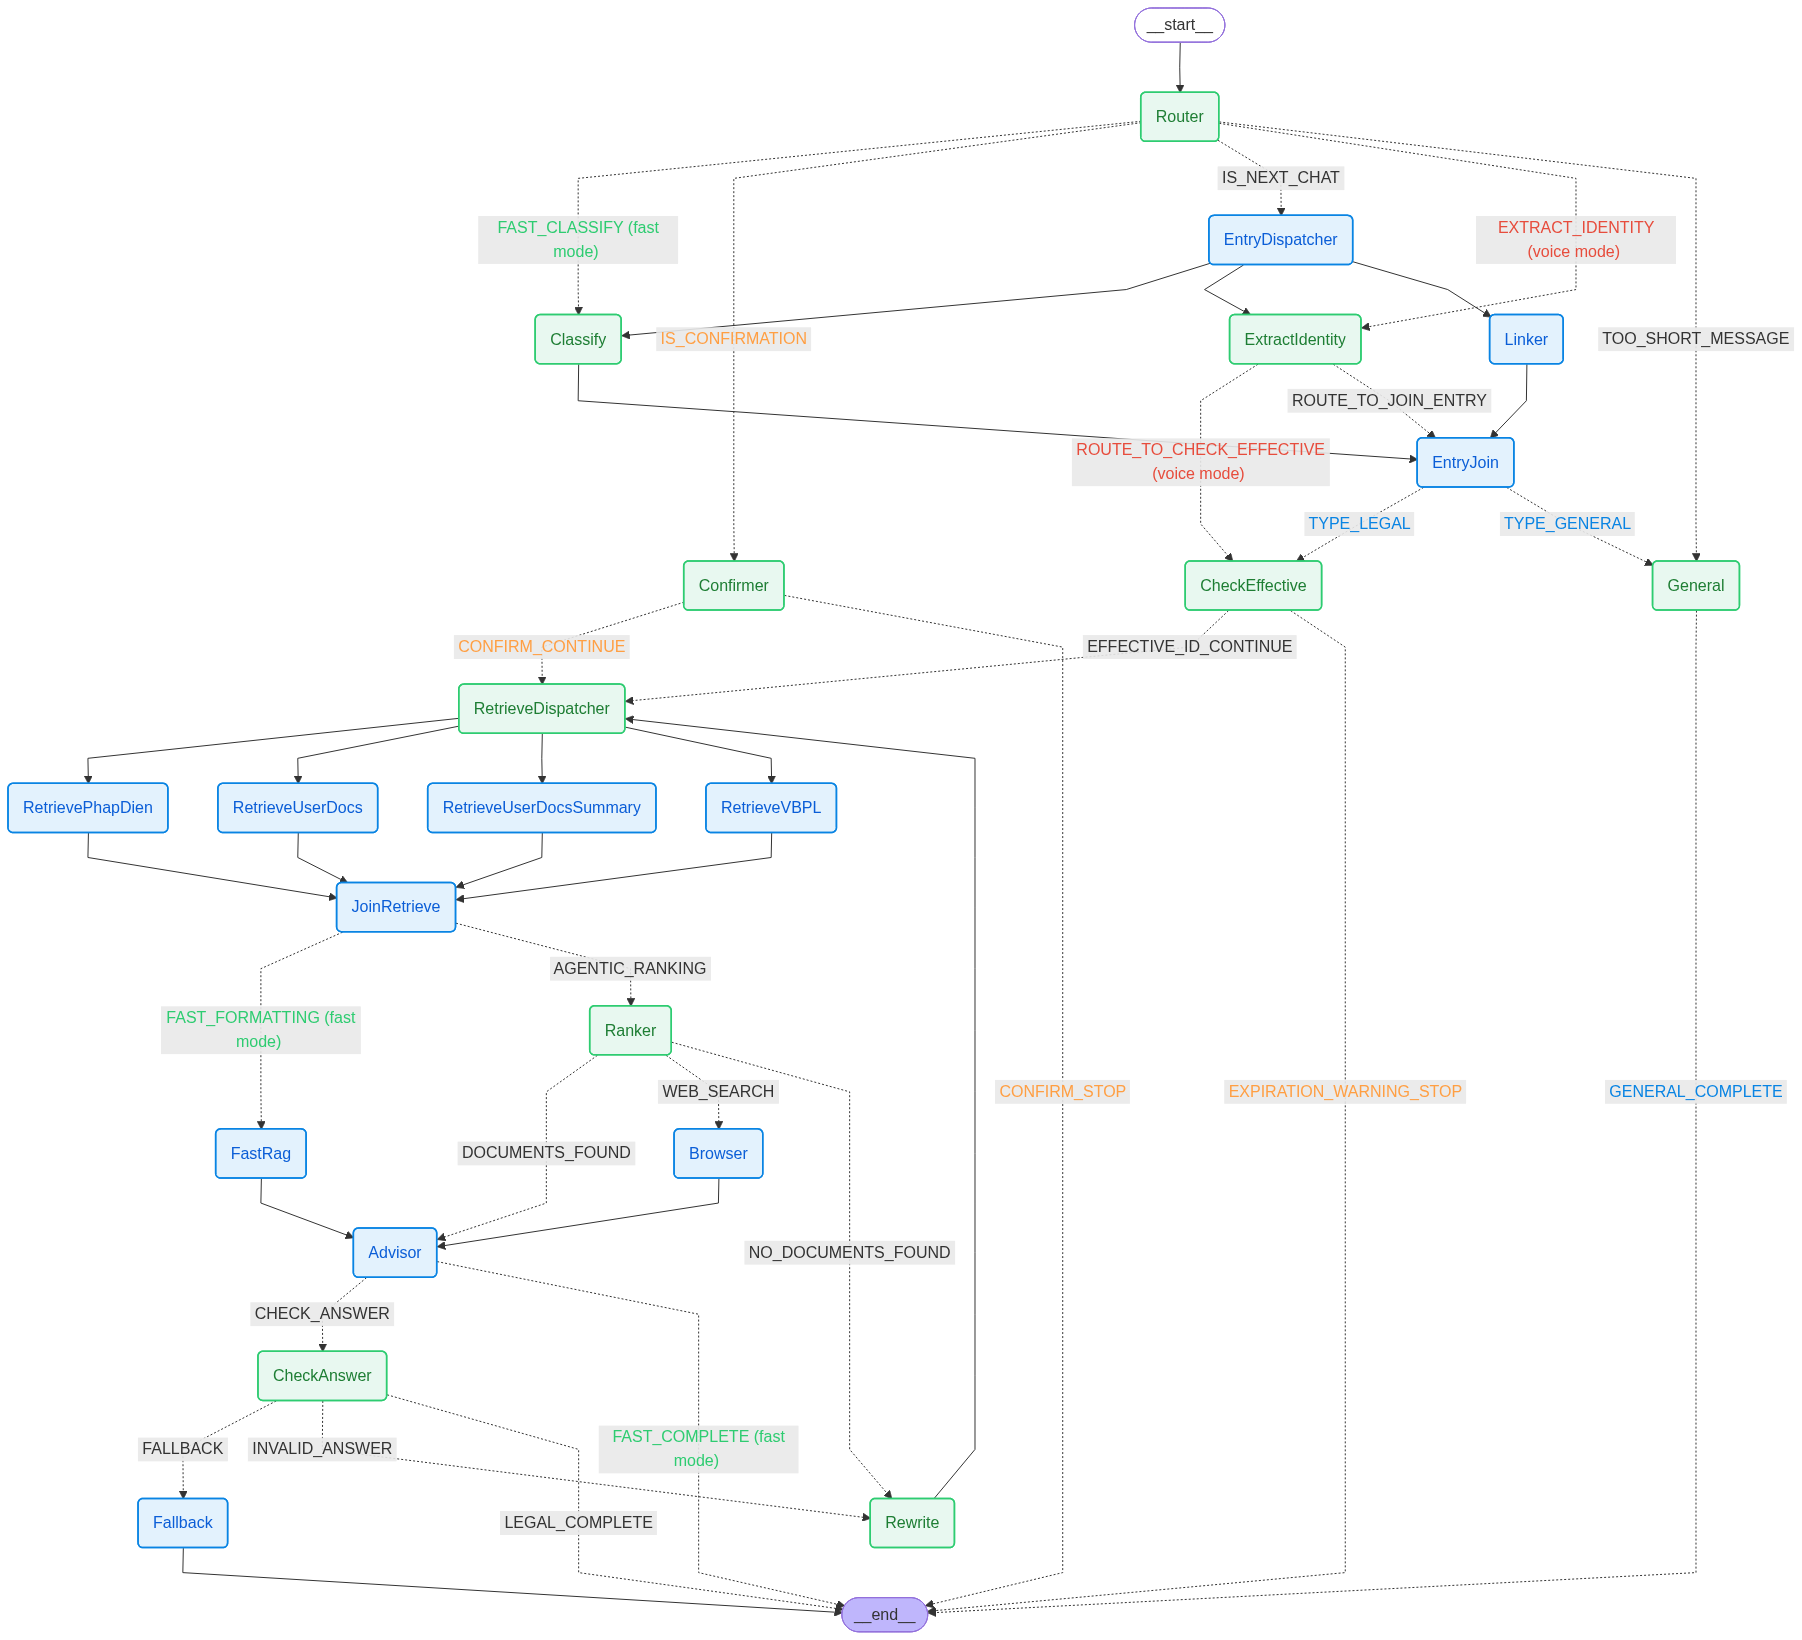
\includegraphics[height=0.55\textheight,width=0.9\textwidth,keepaspectratio]{pictures/rag_diagram.png}
\caption{Sơ đồ LangGraph của dự án}
\end{figure}

\note{
Đây là sơ đồ Agentic RAG của dự án được xây dựng bằng LangGraph. Hệ thống phân chia thông minh giữa mô hình nhỏ cho luồng cơ bản (màu xanh lá) và mô hình lớn cho các tác vụ suy luận phức tạp (màu xanh dương) để tối ưu chi phí và độ trễ.
Mỗi tin nhắn đi qua Router để kiểm tra điều kiện và định tuyến qua các node như rewrite query, retrieve tài liệu và sinh câu trả lời.
}
\end{frame}


% % % \begin{frame}{Tổng quan các dịch vụ}
\begin{figure}[H]
\centering
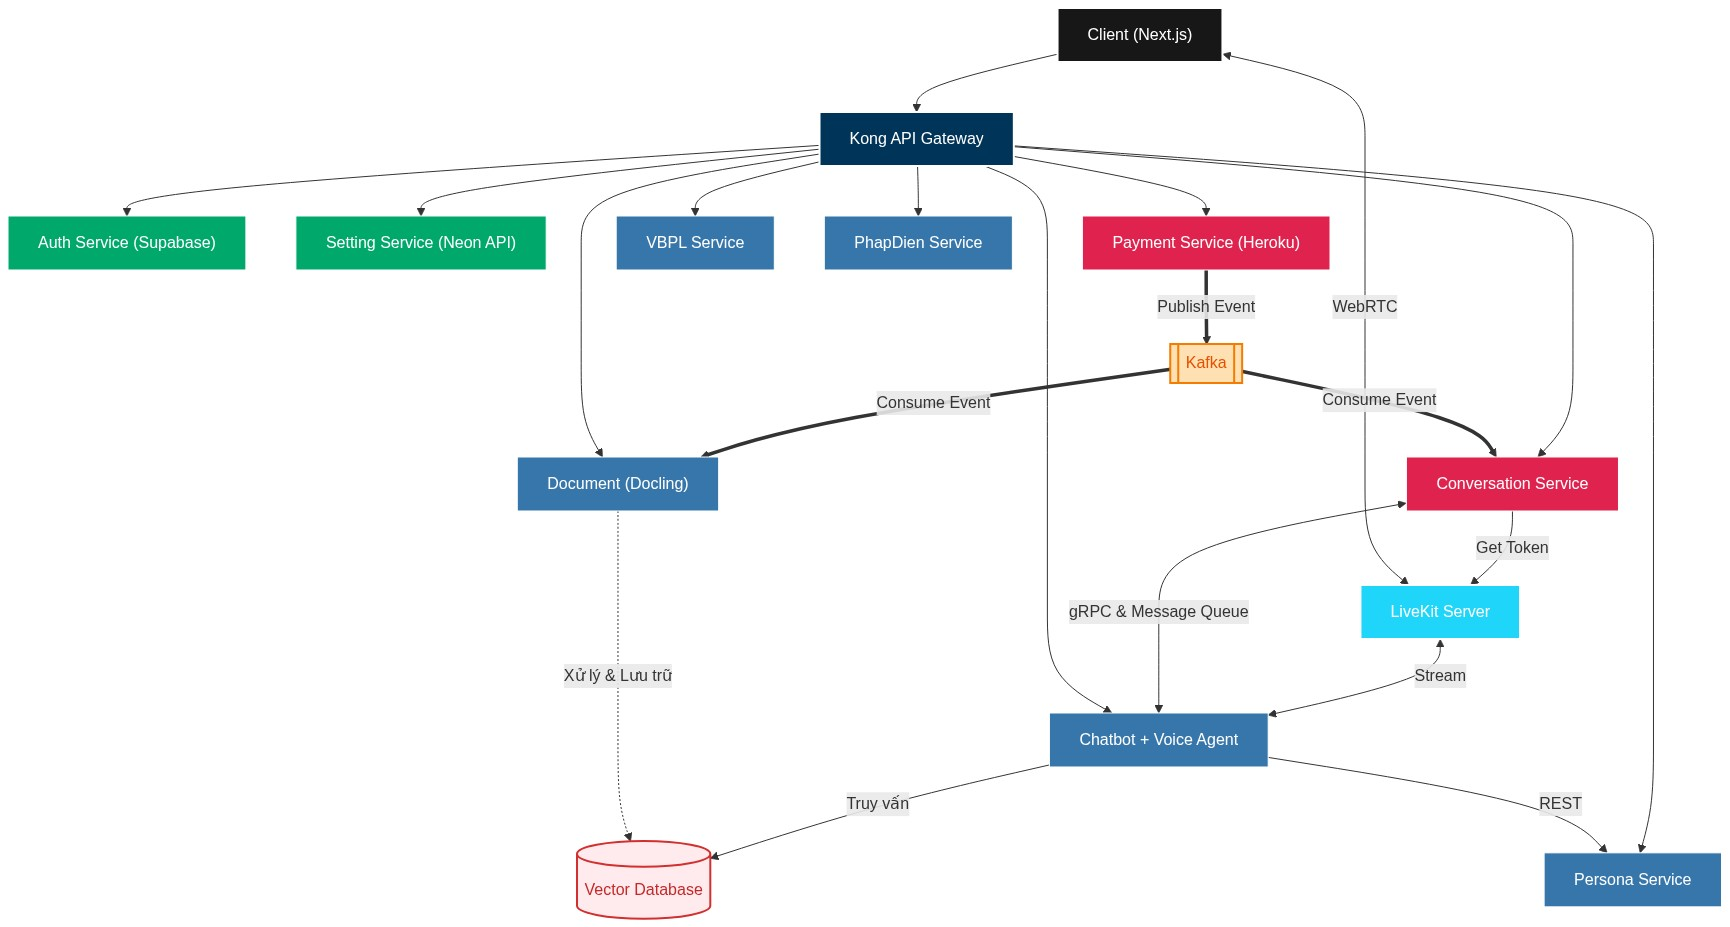
\includegraphics[height=0.7\textheight,width=0.9\textwidth,keepaspectratio]{pictures/MSA.png}
\caption{Tổng quan các dịch vụ của dự án}
\end{figure}

\note{
Sơ đồ tổng quan về kiến trúc các vi dịch vụ được triển khai trong dự án này.
Hệ thống được chia thành nhiều dịch vụ chuyên biệt như: Auth Service (xác thực), Document Service (quản lý tài liệu), Conversation Service (quản lý trò chuyện), Chatbot Service (trí tuệ nhân tạo) và Payment Service (thanh toán). Các dịch vụ này giao tiếp với nhau qua gRPC, REST API hoặc thông điệp bất đồng bộ qua Kafka/RabbitMQ.
}
\end{frame}
% nếu python cash => thanh toán , đăng nhập vẫn không sao

% Nếu các Microservice luôn để xuống service thanh toán


% % \section{Chi tiết các dịch vụ}

% % \begin{frame}{Kiến trúc Dịch vụ Thanh toán (Payment Service)}
\begin{figure}[H]
\centering
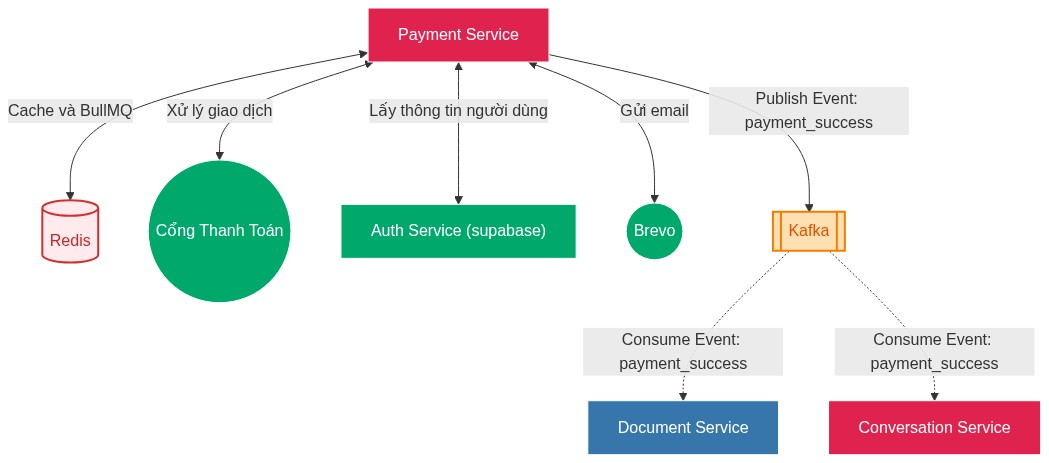
\includegraphics[height=0.7\textheight,width=0.9\textwidth,keepaspectratio]{pictures/payment-kafka-event.png}
\caption{Sơ đồ tổng quan dịch vụ thanh toán}
\end{figure}

\note{
Dịch vụ thanh toán (Payment Service) chịu trách nhiệm quản lý thông tin các gói dịch vụ (Plans), quản lý thuê bao người dùng (Subscriptions) và tích hợp với cổng thanh toán ngoại vi.
Khi người dùng thực hiện thanh toán thành công, dịch vụ này sẽ phát đi sự kiện \texttt{payment\_success} vào hệ thống truyền tin nhắn Kafka để các dịch vụ khác như Chatbot và Document cập nhật quyền VIP cho người dùng.
}
\end{frame}


% % \begin{frame}{Dịch vụ Tài liệu (Document Service)}
\begin{figure}[H]
\centering
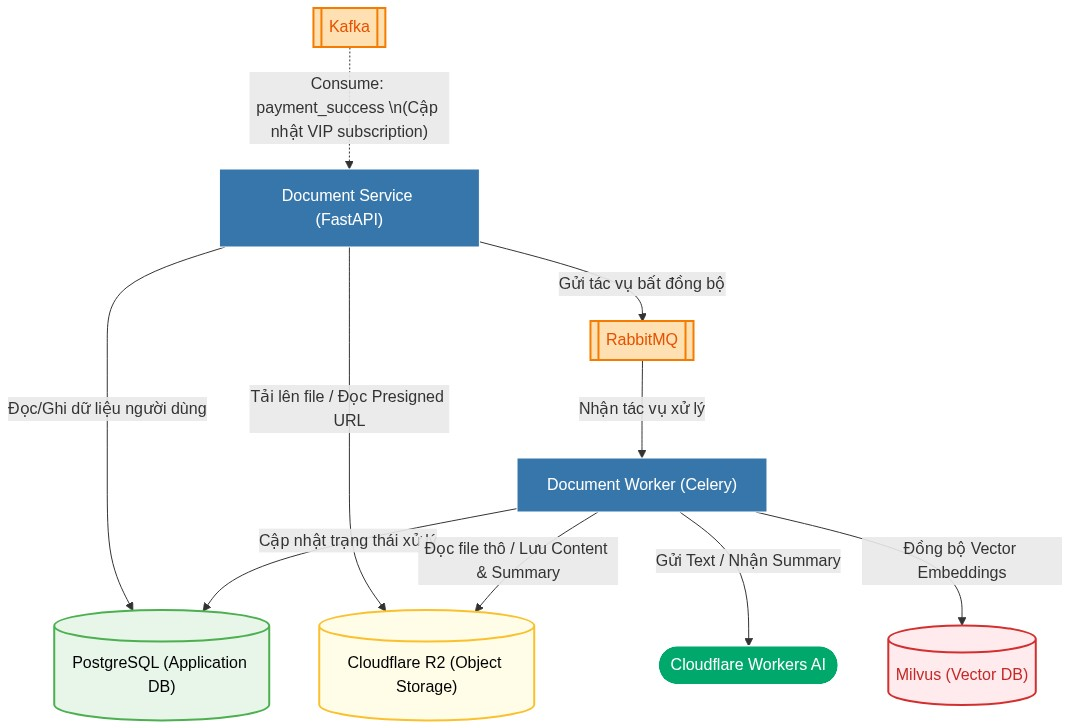
\includegraphics[height=0.7\textheight,width=0.9\textwidth,keepaspectratio]{pictures/document-overview.png}
\caption{Sơ đồ tổng quan dịch vụ văn bản}
\end{figure}

\note{
Dịch vụ tài liệu (Document Service) tiếp nhận, lưu trữ và quản lý tài liệu do người dùng VIP tải lên.
Khi nhận được tệp tin (PDF, DOCX), dịch vụ sẽ gửi yêu cầu xử lý bất đồng bộ thông qua RabbitMQ tới Document Worker. Tài liệu sẽ được trích xuất nội dung sang định dạng Markdown, tự động tóm tắt nội dung chính và tiến hành vector hóa để lưu trữ vào Vector Database Milvus phục vụ cho việc hỏi đáp trên tài liệu.
}
\end{frame}


% % \begin{frame}{Dịch vụ Chatbot và Trò chuyện}
\begin{figure}[H]
\centering
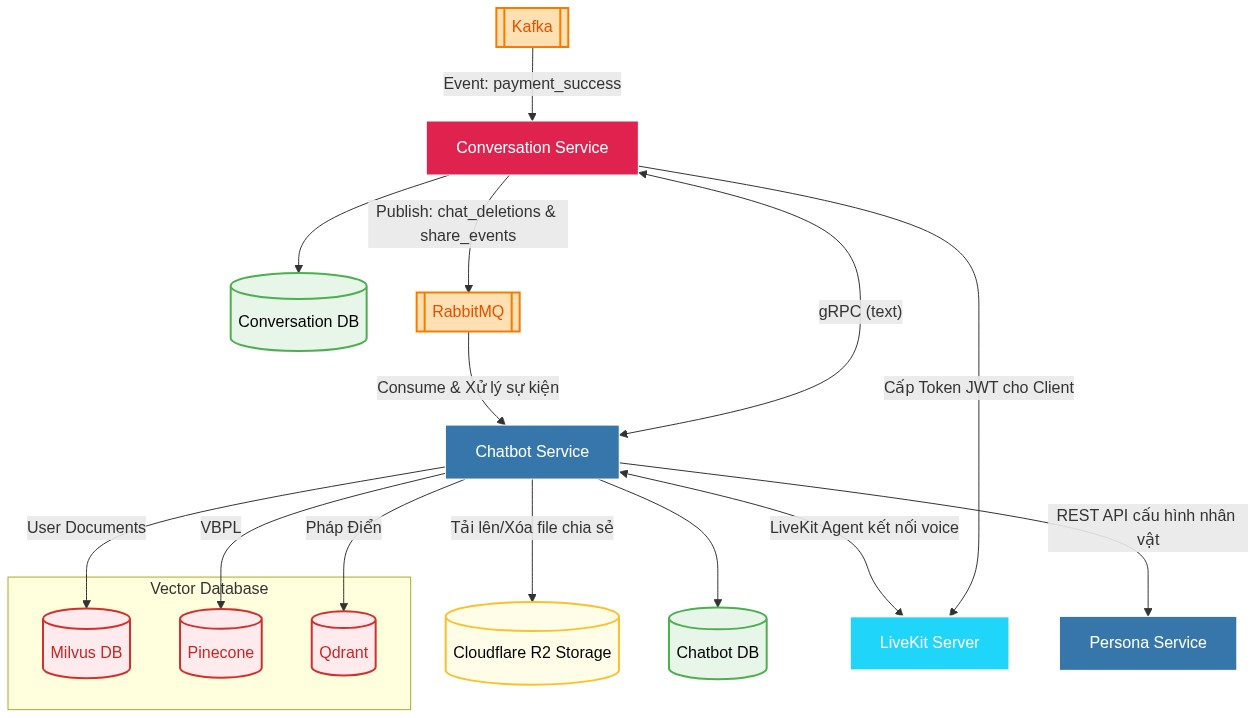
\includegraphics[height=0.7\textheight,width=0.9\textwidth,keepaspectratio]{pictures/conversation-and-chatbot-overview.png}
\caption{Sơ đồ tổng quan dịch vụ trò chuyện và dịch vụ chatbot}
\end{figure}

\note{
Sơ đồ mối quan hệ giữa Dịch vụ trò chuyện (NestJS) và Dịch vụ chatbot (Python).
Dịch vụ trò chuyện chịu trách nhiệm quản lý
trò chuyện của người dùng, lưu trữ lịch sử chat, quản lý thư mục, chia sẻ trò chuyện. Khi có tin nhắn mới, dịch vụ trò chuyện sẽ gửi yêu cầu qua giao thức gRPC hiệu năng cao đến dịch vụ chatbot (Python) để xử lý logic Agentic RAG và trả về câu trả lời dưới dạng stream.
}
\end{frame}


% % \begin{frame}{Kiến trúc tích hợp đàm thoại thời gian thực (Voice Agent)}
\begin{figure}[H]
\centering
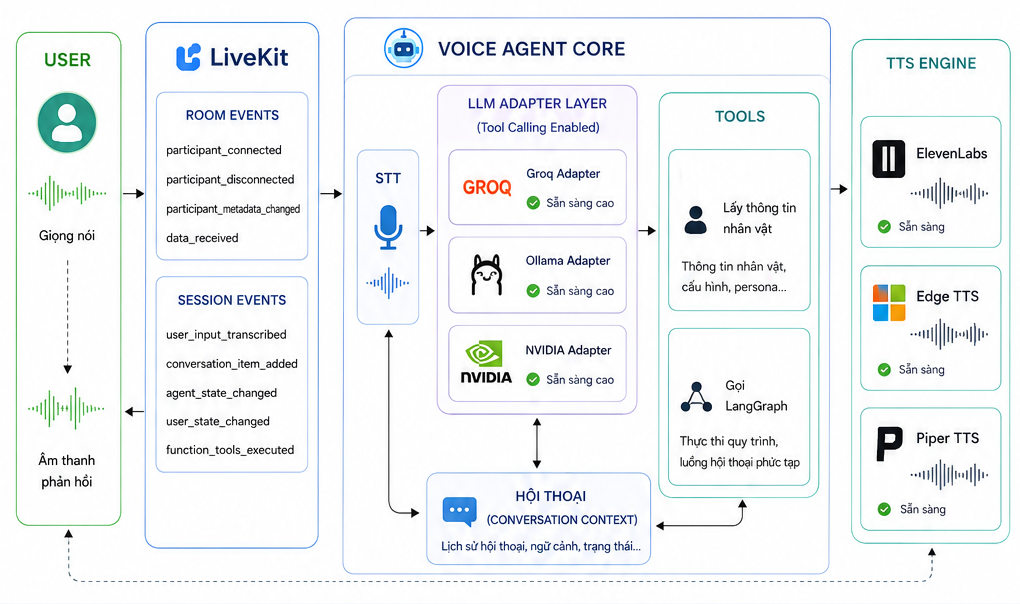
\includegraphics[height=0.7\textheight,width=0.9\textwidth,keepaspectratio]{pictures/voice-livekit-overview.png}
\caption{Sơ đồ tích hợp LiveKit đàm thoại giọng nói}
\end{figure}

\note{
Hệ thống tích hợp máy chủ LiveKit để cung cấp tính năng đàm thoại giọng nói thời gian thực với trợ lý ảo.
Khi người dùng kết nối, Voice Agent hoạt động như một LiveKit Agent, chủ động kết nối và trao đổi âm thanh hai chiều thông qua giao thức WebRTC. Voice Agent tích hợp các mô hình VAD (phát hiện giọng nói), STT (chuyển giọng nói thành văn bản), LLM (suy luận phản hồi) và TTS (chuyển văn bản thành giọng nói) với độ trễ cực thấp.
}
\end{frame}


% \ifdev
% \begin{frame}
\frametitle{}
\maketitle
\end{frame}

\begin{frame}{Cảm ơn}
\centering
\Huge{Thanks for listening!}
\end{frame}

\begin{frame}{Cảm ơn}
\centering
\Huge{Thanks for listening!}
\end{frame}

% \fi

\section{Các công nghệ khác}

\input{contents/Quy_trinh_tu_dong_hoa_CICD_bang_GitHub_Actions}
\begin{frame}{Quản lý Hạ tầng dưới dạng mã}
\begin{figure}[H]
\centering
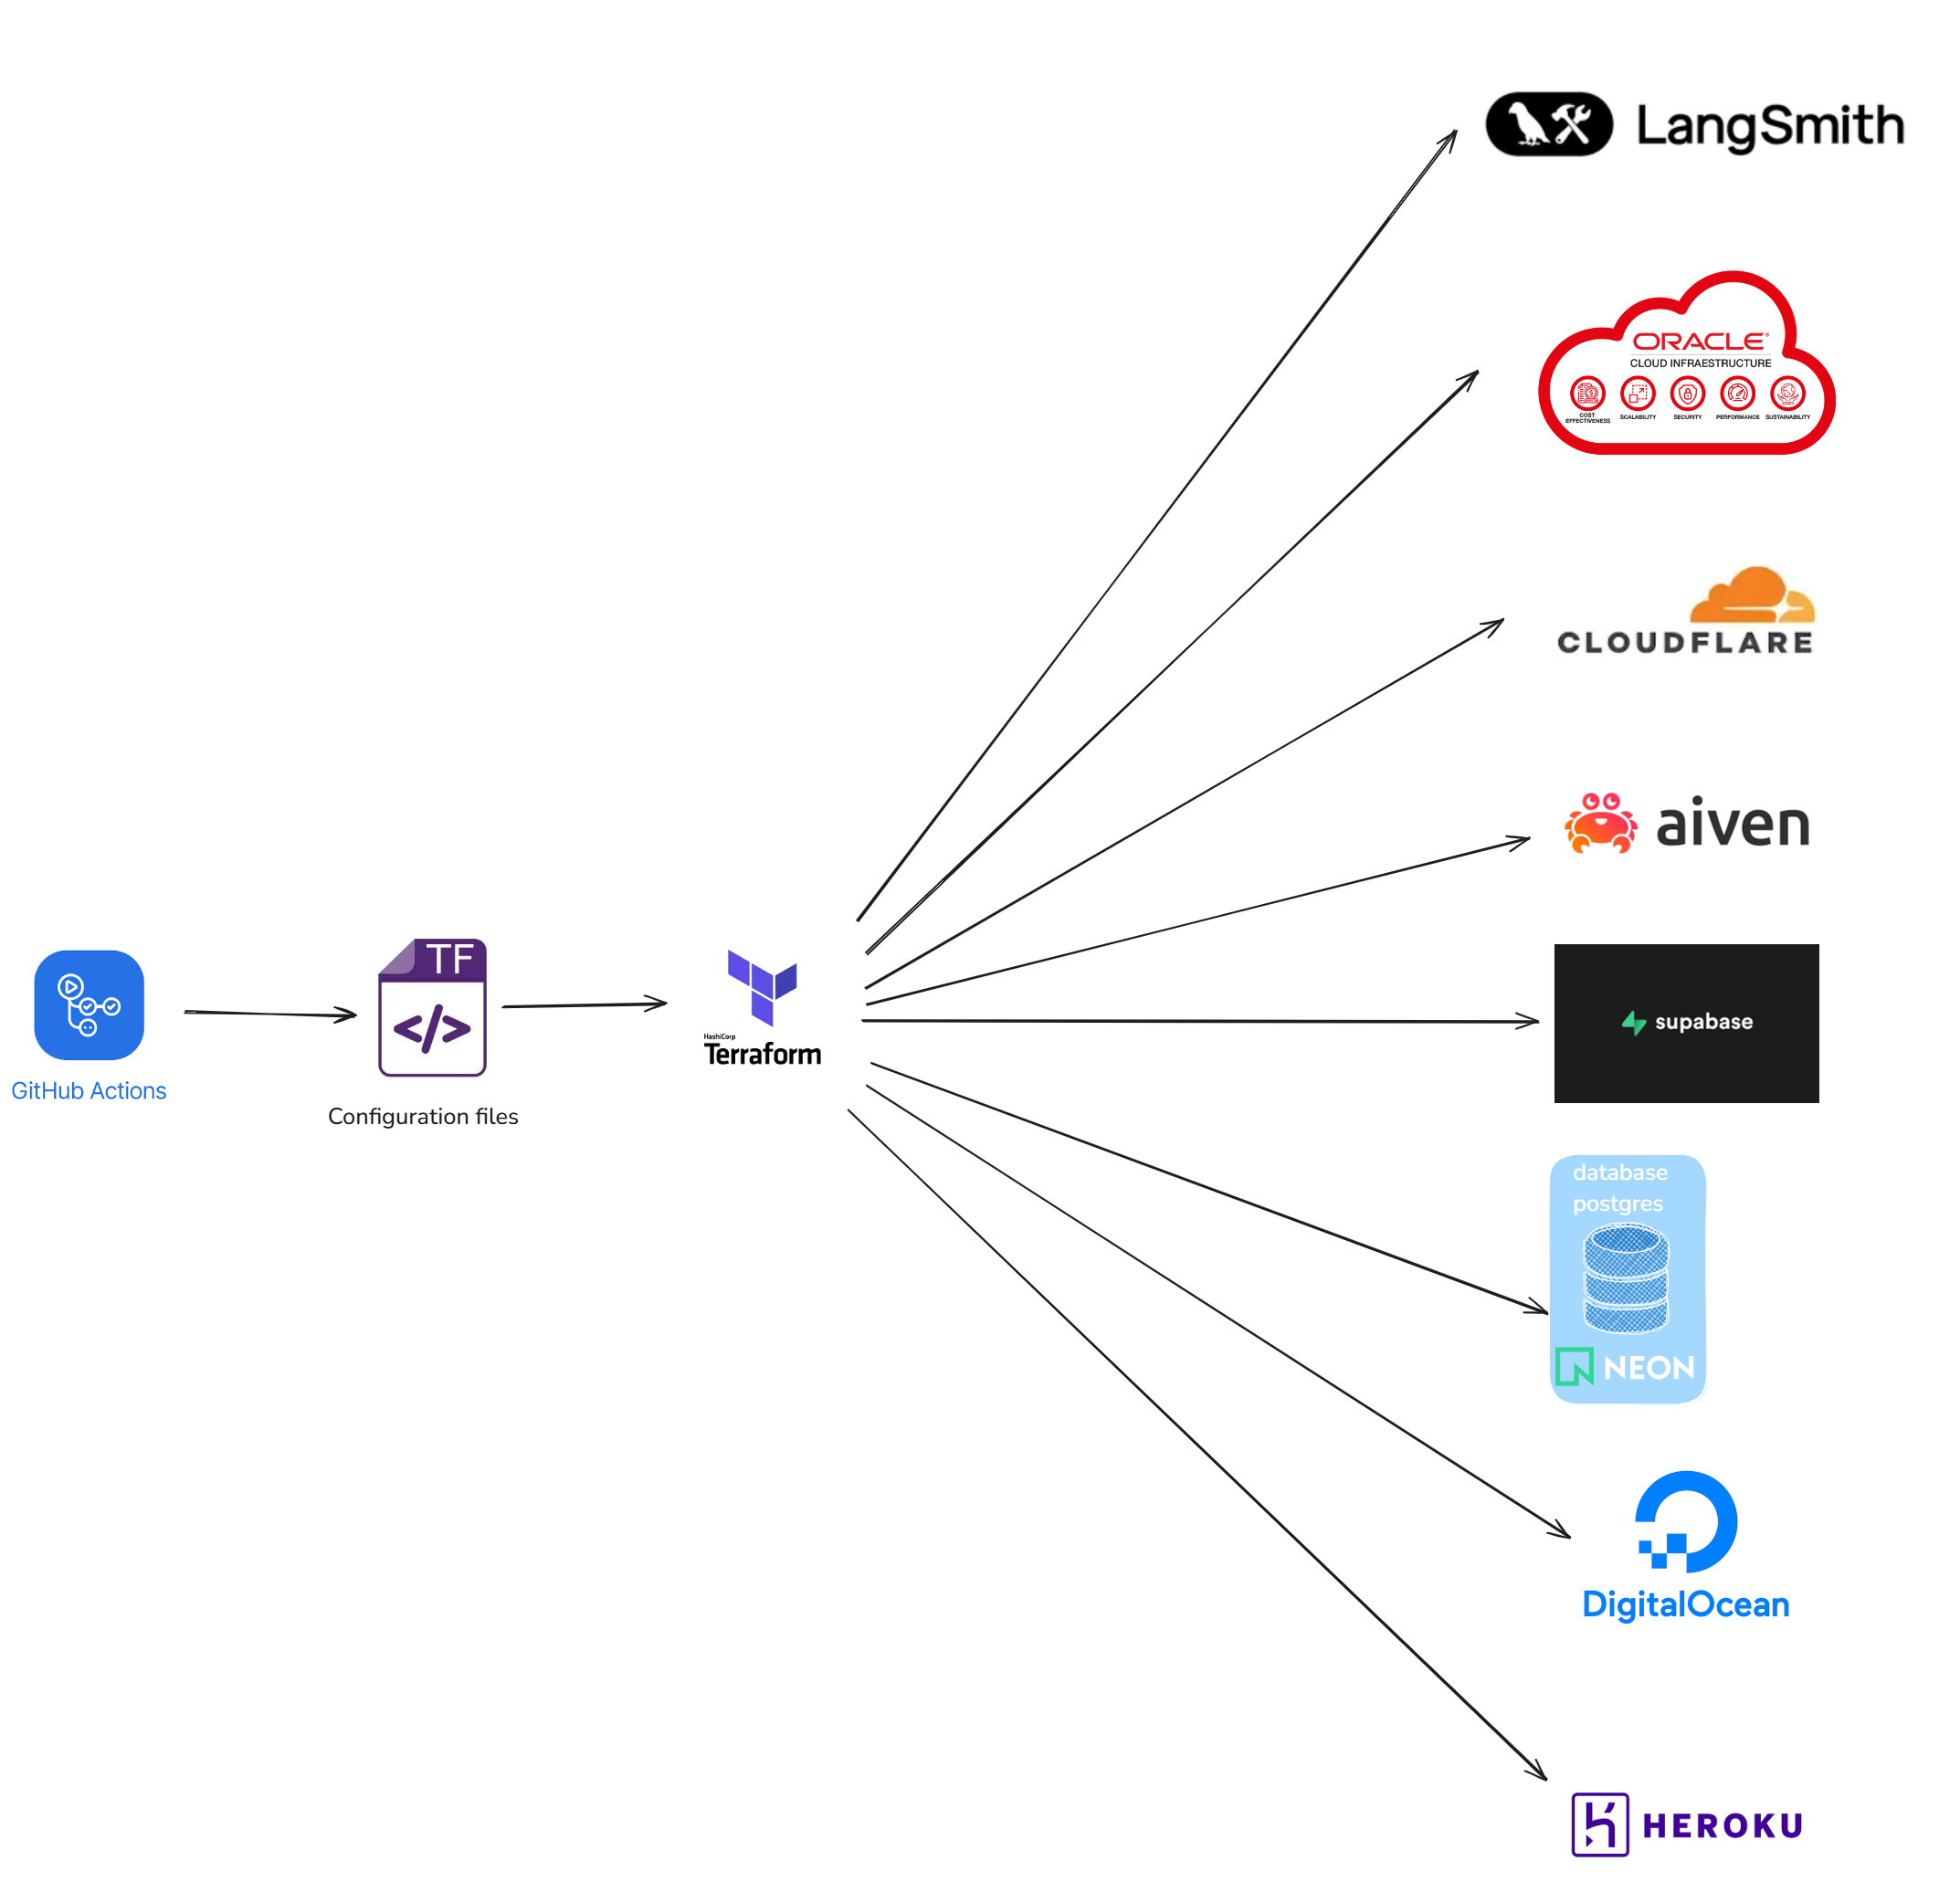
\includegraphics[height=0.7\textheight,width=0.9\textwidth,keepaspectratio]{pictures/infrastructure-as-code-IaC-terraform.excalidraw.png}
\caption{Sơ đồ tổng quan quản lý hạ tầng bằng Terraform trong dự án}
\end{figure}

\note{
Để quản lý hạ tầng một cách nhất quán và tự động, dự án sử dụng Terraform dưới dạng Infrastructure as Code (IaC).
Terraform tự động khởi tạo và cấu hình các tài nguyên bên thứ ba như: Supabase (Auth), LangSmith (giám sát RAG), Cloudflare (DNS và R2 Storage), Neon (PostgreSQL cho các vi dịch vụ), DigitalOcean (Crawl DB) và Heroku (Payment Service). Trạng thái hạ tầng được lưu trữ tập trung trên Terraform Cloud.
}
\end{frame}

\input{contents/Cau_hinh_Kong_API_Gateway_bang_Declarative_Configuration}
\begin{frame}{Kết quả Docker Image trên Docker Hub}
\begin{figure}[H]
\centering
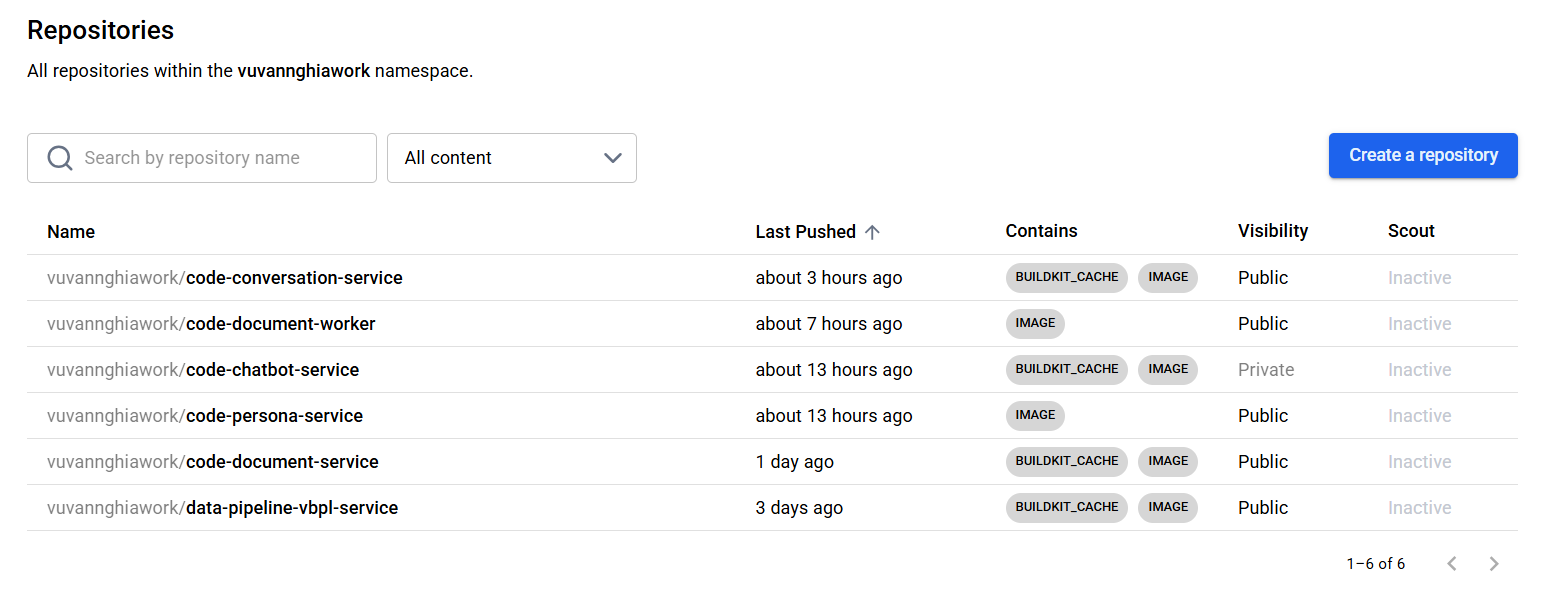
\includegraphics[height=0.55\textheight,width=0.9\textwidth,keepaspectratio]{pictures/docker-hub-web-ui2.png}
\caption{Kết quả Docker Image được push lên Docker Hub}
% \caption{Kết quả giao diện docker}
\end{figure}

\note{
docker
}
\end{frame}

\begin{frame}{Cấu hình tài nguyên Kubernetes trong GitOps Repository}
\begin{figure}[H]
\centering
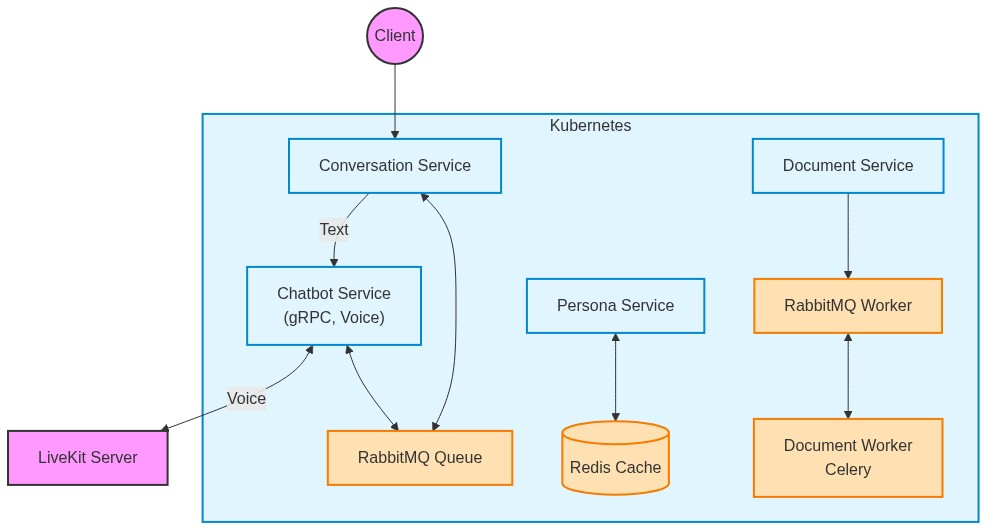
\includegraphics[height=0.55\textheight,width=0.9\textwidth,keepaspectratio]{pictures/Kubernetes.png}
\caption{Cấu hình Kubernetes trong kho lưu trữ GitOps của dự án}
\end{figure}

\note{
Đây là cấu trúc thư mục chứa các file cấu hình Kubernetes (YAML) trong kho lưu trữ GitOps của dự án.
Các dịch vụ nội bộ như RabbitMQ, Redis được chạy trực tiếp trong cụm để giảm độ trễ và được cấu hình dưới dạng ClusterIP để tăng tính bảo mật, ngăn chặn các truy cập trực tiếp từ internet. Các dịch vụ chạy bất đồng bộ như Voice Agent hay Document Worker cũng không công khai service ra bên ngoài.
}
\end{frame}


\begin{frame}{Giao diện quản lý GitOps bằng ArgoCD}
\begin{figure}[H]
\centering
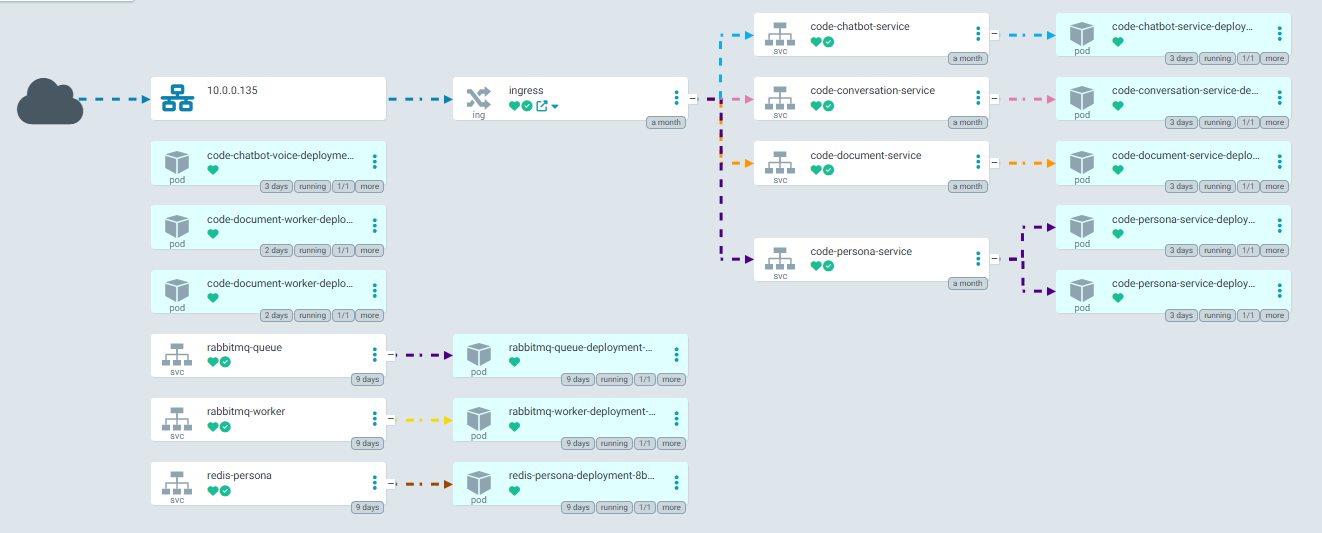
\includegraphics[height=0.55\textheight,width=0.9\textwidth,keepaspectratio]{pictures/argocd-web-ui.png}
\caption{Kết quả giao diện ArgoCD chạy docker trong kubernetes}
\end{figure}

\note{
ArgoCD được triển khai trong cụm Kubernetes để thực hiện quy trình Continuous Delivery (CD) theo mô hình GitOps.
ArgoCD liên tục giám sát kho lưu trữ Git chứa các file cấu hình Kubernetes. Khi phát hiện có sự thay đổi (ví dụ: phiên bản Docker image mới), ArgoCD sẽ tự động đồng bộ (sync) và cập nhật các Pod đang chạy trên Kubernetes thực tế để khớp với cấu hình được khai báo trên Git.
}
\end{frame}


%%%%%%%%%%%%%%%%%%%%%%%%%%%%%%%%%%%%%%%%%%%%%%%%%%%%%%%
\newpage
\phantomsection
{\centering \section*{KẾT LUẬN}}
\addcontentsline{toc}{section}{KẾT LUẬN}

\subsection*{Kết luận}

Sau thời gian nghiên cứu,
thiết kế và phát triển,
đồ án tốt nghiệp
đã hoàn thành đầy đủ các mục tiêu đề ra ban đầu,
đáp ứng toàn bộ các yêu cầu kỹ thuật
và nghiệp vụ được giao.

Về kết quả đạt được, đồ án đã mang lại các giá trị cụ thể như sau:

\begin{itemize}
\item \textbf{Về mặt sản phẩm:}
Xây dựng thành công một hệ thống trợ lý pháp luật hoàn chỉnh
hoạt động dựa trên kiến trúc vi dịch vụ
ổn định và dễ mở rộng.
Trợ lý AI sử dụng giải pháp Agentic RAG tiên tiến với LangGraph,
cho phép trả lời các truy vấn pháp lý tiếng Việt một cách chính xác,
minh bạch qua luồng suy luận rõ ràng và dẫn nguồn từ CSDL pháp điển cũng như văn bản quy phạm pháp luật chính thống.
Đồng thời, hệ thống hỗ trợ đàm thoại giọng nói thời gian thực, xử lý tài liệu người dùng và tự động hóa quy trình thanh toán.

\item \textbf{Về mặt công nghệ:}
Tích hợp và làm chủ nhiều giải pháp công nghệ hiện đại:
xây dựng hệ thống trên nền tảng kiến trúc vi dịch vụ
có ứng dụng Domain-Driven Design,
vận hành qua Kong API Gateway
với các giao thức giao tiếp REST, gRPC
cùng hệ thống hàng đợi RabbitMQ, Kafka.
Thiết lập lưu trữ đa dạng sử dụng postgres
kết hợp các CSDL vector (Qdrant, Pinecone, Milvus)
cùng các kho lưu trữ Supabase Storage, Cloudflare R2, Google Drive.
Xây dựng các đường ống thu thập dữ liệu
tự động nhờ cron-job.org, GitHub Actions, Scrapy và dlt.
Triển khai giải pháp Agentic RAG nâng cao bằng LangGraph
kết hợp các mô hình ngôn ngữ lớn
và HuggingFace (vietnamese-sbert).
Tích hợp hệ thống xác thực bảo mật qua Supabase (JWT, Google OAuth, 2FA/TOTP)
cùng phân hệ đàm thoại giọng nói LiveKit
và các công cụ TTS (edge-tts, piper-tts, ElevenLabs).
Toàn bộ hệ thống được đóng gói bằng Docker,
điều phối vận hành trên Kubernetes
thông qua quy trình CI/CD của GitHub Actions
và đồng bộ hóa hạ tầng tự động theo mô hình GitOps với ArgoCD.

\item \textbf{Về mặt kiến thức và kỹ năng tích lũy:}
Qua quá trình thực hiện đồ án,
sinh viên đã tích lũy được nhiều kiến thức
về
mô hình ngôn ngữ lớn,
kiến trúc hệ thống phân tán
và quy trình vận hành DevOps/GitOps.
Đồng thời, sinh viên phát triển
và nâng cao các kỹ năng như:
kỹ năng nghiên cứu khoa học,
tìm kiếm và tổng hợp tài liệu,
kỹ năng lập kế hoạch và quản lý dự án.

\end{itemize}

Về mặt đánh giá,
hệ thống cho thấy tính thực tiễn
khi giải quyết được bài toán tra cứu
thông tin pháp luật phức tạp.
Tuy nhiên, tính chính xác của câu trả lời phụ thuộc nhiều
vào chất lượng và độ cập nhật của CSDL nguồn.
Các mô hình AI vẫn đóng vai trò
là một trợ lý hỗ trợ đắc lực
và không thể thay thế hoàn toàn vai trò của các chuyên gia pháp lý
trong các tình huống quyết định mang tính pháp lý cao.

\subsection*{Hướng phát triển}

Để hoàn thiện ứng dụng
và nâng cao khả năng
phục vụ người dùng trong thực tế,
hướng phát triển của đồ án
trong tương lai tập trung vào các nội dung sau:

\begin{itemize}

\item \textbf{Nâng cao chất lượng AI và tối ưu hóa hệ thống RAG:}
Nghiên cứu
huấn luyện tinh chỉnh
mô hình ngôn ngữ lớn
trên các tập dữ liệu đặc thù của pháp luật Việt Nam
để nâng cao độ chính xác
và khả năng lập luận chuyên sâu.

\item \textbf{Nâng cấp khả năng điều phối luồng dữ liệu:}
Tích hợp Airflow vào quy trình xử lý dữ liệu
để tự động hóa và giám sát đường ống dữ liệu.
Sử dụng đồ thị định hướng không chu trình
(Directed Acyclic Graph - DAG)
để định nghĩa các luồng logic phức tạp dựa trên điều kiện thực tế của dữ liệu.

\item \textbf{Đánh giá và kiểm soát chất lượng mô hình AI:}
Ứng dụng khung đánh giá RAGAS
(Retrieval Augmented Generation Assessment)
để đo lường các chỉ số chất lượng của hệ thống RAG.
Từ đó, tiến hành tinh chỉnh và cấu hình các ngưỡng phản hồi
hợp lý nhằm đảm bảo tính an toàn,
chính xác và đáng tin cậy của mô hình
trước khi trả về kết quả cho người dùng.

\item \textbf{Đảm bảo chất lượng phần mềm:}
Triển khai công cụ Playwright
để xây dựng các kịch bản kiểm thử tự động
toàn diện cho cả giao diện người dùng
và các API,
giúp phát hiện lỗi sớm
và đảm bảo hệ thống hoạt động ổn định.

\item \textbf{Mở rộng phân hệ thanh toán và tài chính:}
Phát triển thêm tính năng xuất hóa đơn
điện tử phục vụ đối tượng khách hàng doanh nghiệp
và xây dựng chức năng mã giảm giá cần
xử lý thêm bài toán nhiều người
sử dụng mã giảm giá cùng lúc,
đồng thời tích hợp thêm cổng thanh toán Stripe
nhằm đáp ứng nhu cầu của tệp khách hàng quốc tế.

\item \textbf{Tối ưu hóa trải nghiệm đàm thoại giọng nói (Voice Bot):}
Nâng cấp các dịch vụ chuyển đổi giọng nói
cao cấp
hoặc tự triển khai các mô hình AI trên máy chủ có hỗ trợ GPU
nhằm giảm thiểu tối đa độ trễ, mang lại trải nghiệm đàm thoại mượt mà và tự nhiên cho người dùng.

\item \textbf{Nâng cao khả năng xử lý tài liệu đa định dạng:}
Tích hợp các công nghệ trích xuất thông tin
và đọc hiểu tài liệu tiên tiến
để hệ thống có thể xử lý đa dạng các định dạng tệp tin.

\item \textbf{Mở rộng và tối ưu hóa hạ tầng điện toán đám mây:}
Triển khai
trên môi trường đa cụm Kubernetes
nhằm tăng cường tính sẵn sàng,
đồng thời tối ưu hóa các quy trình tự động co giãn
giúp hệ thống vận hành ổn định trước lượng lớn người dùng truy cập đồng thời.

\item \textbf{Xây dựng hệ thống giám sát và quản lý nhật ký tập trung (Observability):}
Triển khai giải pháp giám sát toàn diện cho kiến trúc vi dịch vụ
bằng cách tích hợp Prometheus để thu thập số liệu hiệu năng (metrics)
hệ thống theo thời gian thực
và Grafana để trực quan hóa trạng thái vận hành, thiết lập các kịch bản cảnh báo tự động.
Đồng thời, ứng dụng bộ công cụ ELK Stack
(Elasticsearch, Logstash, Kibana)
làm giải pháp quản lý nhật ký (logging) tập trung,
hỗ trợ thu thập, tiền xử lý và phân tích log
từ tất cả các vi dịch vụ, từ đó tối ưu hóa quy trình
định vị sự cố (troubleshooting) và đảm bảo tính sẵn sàng cao cho hệ thống.

\end{itemize}
\newpage

\newpage
\phantomsection
{\centering \section*{TÀI LIỆU THAM KHẢO}}
\addcontentsline{toc}{section}{TÀI LIỆU THAM KHẢO}

\begingroup
\renewcommand{\section}[2]{} % Bỏ qua lệnh tạo tiêu đề tự động của thebibliography
\begin{thebibliography}{00}

\bibitem{vaswani2017attention}
Vaswani, A., Shazeer, N., Parmar, N., Uszkoreit, J., Jones, L., Gomez, A. N., Kaiser, L., \& Polosukhin, I. (2017). Attention is all you need. \textit{Advances in neural information processing systems}, 30. \url{http://arxiv.org/abs/1706.03762}

\bibitem{ARSLAN20243781}
Arslan, M., Ghanem, H., Munawar, S., \& Cruz, C. (2024). A Survey on RAG with LLMs. \textit{Procedia Computer Science}, 246, 3781-3790. \url{https://doi.org/10.1016/j.procs.2024.09.178}

\bibitem{agentic-ai-2026}
Dwivedi, Y. K., et al. (2026). Agentic AI Systems: What It Is and Isn't. \textit{Global Business and Organizational Excellence}, 45(3), 253-263. \url{https://doi.org/10.1002/joe.70018}

\bibitem{ddd-evans}
Evans, E. (2004). \textit{Domain-Driven Design: Tackling Complexity in the Heart of Software}. Addison-Wesley Professional.

\bibitem{ddd-quickly}
Marinescu, F., \& Abel, A. (2006). \textit{Domain-Driven Design Quickly}. C4Media.

\bibitem{fowler-event-driven}
Fowler, M. (2017). \textit{What do you mean by "Event-Driven"?}. Truy cập ngày 28/06/2026, từ \url{https://martinfowler.com/articles/201701-event-driven.html}

\bibitem{outbox-pattern}
Richardson, C. \textit{Pattern: Transactional outbox}. Microservices.io. Truy cập ngày 28/06/2026, từ \url{https://microservices.io/patterns/data/transactional-outbox.html}

\bibitem{aws-rag}
Amazon Web Services. \textit{Retrieval-Augmented Generation (RAG) là gì?}. Truy cập ngày 28/06/2026, từ \url{https://aws.amazon.com/vi/what-is/retrieval-augmented-generation}

\bibitem{weaviate-rag}
Weaviate. \textit{What is Agentic RAG?}. Truy cập ngày 28/06/2026, từ \url{https://weaviate.io/blog/what-is-agentic-rag}

\bibitem{dlthub}
dltHub. \textit{Introduction to dlt}. Truy cập ngày 28/06/2026, từ \url{https://dlthub.com/docs/intro}

\bibitem{scrapy}
Scrapy. \textit{A Fast and Powerful Scraping and Web Crawling Framework}. Truy cập ngày 28/06/2026, từ \url{https://www.scrapy.org}

\bibitem{vbpl}
Cơ sở dữ liệu Quốc gia về Văn bản Pháp luật. Truy cập ngày 28/06/2026, từ \url{https://vbpl.vn}

\bibitem{phapdien}
Bộ Tư pháp. \textit{Chi tiết Bộ Pháp điển}. Truy cập ngày 28/06/2026, từ \url{https://phapdien.moj.gov.vn/Pages/chi-tiet-bo-phap-dien.aspx}

\bibitem{vietnamese-sbert}
Hugging Face. \textit{vietnamese-sbert}. Truy cập ngày 28/06/2026, từ \url{https://huggingface.co/keepitreal/vietnamese-sbert}

\bibitem{langchain-vectorstores}
LangChain. \textit{Vector stores}. Truy cập ngày 28/06/2026, từ \url{https://docs.langchain.com/oss/python/integrations/vectorstores}

\bibitem{langgraph}
LangChain. \textit{LangGraph Overview}. Truy cập ngày 28/06/2026, từ \url{https://docs.langchain.com/oss/python/langgraph/overview}

\bibitem{ddd-hexagon}
Sairyss. \textit{Domain-Driven Hexagon}. GitHub. Truy cập ngày 28/06/2026, từ \url{https://github.com/Sairyss/domain-driven-hexagon#diagram}

\bibitem{doppler-branch}
Doppler. \textit{Branch Configs}. Truy cập ngày 28/06/2026, từ \url{https://docs.doppler.com/docs/branch-configs}

\bibitem{kong-gateway}
Kong. \textit{Kong Gateway}. Truy cập ngày 28/06/2026, từ \url{https://developer.konghq.com/gateway}

\bibitem{supabase-storage}
Supabase. \textit{Storage Guides}. Truy cập ngày 28/06/2026, từ \url{https://supabase.com/docs/guides/storage}

\bibitem{supabase-totp}
Supabase. \textit{Time-based One-Time Passwords (TOTP)}. Truy cập ngày 28/06/2026, từ \url{https://supabase.com/docs/guides/auth/auth-mfa/totp}

\bibitem{supabase-jwts}
Supabase. \textit{JSON Web Tokens (JWTs)}. Truy cập ngày 28/06/2026, từ \url{https://supabase.com/docs/guides/auth/jwts}

\bibitem{neon-postgrest}
Neon. \textit{Create a REST API from Postgres with PostgREST}. Truy cập ngày 28/06/2026, từ \url{https://neon.com/docs/guides/postgrest}

\bibitem{heroku-docker}
Heroku. \textit{Deploying with Docker}. Truy cập ngày 28/06/2026, từ \url{https://devcenter.heroku.com/categories/deploying-with-docker}

\bibitem{momo-notification}
MoMo. \textit{Payment Notification}. Truy cập ngày 28/06/2026, từ \url{https://developers.momo.vn/v3/vi/docs/payment/api/result-handling/notification/}

\bibitem{nestjs-cqrs}
NestJS. \textit{CQRS}. Truy cập ngày 28/06/2026, từ \url{https://docs.nestjs.com/recipes/cqrs}

\bibitem{nestjs-sse}
NestJS. \textit{Server-Sent Events}. Truy cập ngày 28/06/2026, từ \url{https://docs.nestjs.com/techniques/server-sent-events}

\bibitem{typeorm-migrations}
TypeORM. \textit{How migrations work?}. Truy cập ngày 28/06/2026, từ \url{https://typeorm.io/docs/migrations/why}

\bibitem{alembic-autogenerate}
Alembic. \textit{Auto Generating Migrations}. Truy cập ngày 28/06/2026, từ \url{https://alembic.sqlalchemy.org/en/latest/autogenerate.html}

\bibitem{fastapi}
FastAPI. \textit{FastAPI Framework}. Truy cập ngày 28/06/2026, từ \url{https://fastapi.tiangolo.com}

\bibitem{testcontainers}
Testcontainers. \textit{Testcontainers}. Truy cập ngày 28/06/2026, từ \url{https://testcontainers.com}

\bibitem{docling}
Docling. \textit{Docling AI}. Truy cập ngày 28/06/2026, từ \url{https://www.docling.ai}

\bibitem{langfuse-langsmith}
Langfuse. \textit{LangSmith Alternative}. Truy cập ngày 28/06/2026, từ \url{https://langfuse.com/resources/engineering/langsmith-alternative}

\bibitem{bullmq}
BullMQ. \textit{BullMQ Documentation}. Truy cập ngày 28/06/2026, từ \url{https://docs.bullmq.io}

\bibitem{celeryq-rabbitmq}
Celery. \textit{Using RabbitMQ}. Truy cập ngày 28/06/2026, từ \url{https://docs.celeryq.dev/en/v5.5.3/getting-started/backends-and-brokers/rabbitmq.html}

\bibitem{rabbitmq-dlx}
RabbitMQ. \textit{Dead Letter Exchanges}. Truy cập ngày 28/06/2026, từ \url{https://www.rabbitmq.com/docs/dlx}

\bibitem{kafka-design}
Apache Kafka. \textit{Design}. Truy cập ngày 28/06/2026, từ \url{https://kafka.apache.org/43/design/design}

\bibitem{github-actions}
GitHub. \textit{GitHub Actions Documentation}. Truy cập ngày 28/06/2026, từ \url{https://docs.github.com/en/actions}

\bibitem{terraform}
HashiCorp. \textit{Terraform Documentation}. Truy cập ngày 28/06/2026, từ \url{https://developer.hashicorp.com/terraform}

\bibitem{neon-auth}
Neon. \textit{Custom Authentication Providers}. Truy cập ngày 28/06/2026, từ \url{https://neon.com/docs/data-api/custom-authentication-providers}

\bibitem{grpc-docs}
gRPC. \textit{gRPC Documentation}. Truy cập ngày 28/06/2026, từ \url{https://grpc.io/docs}

\bibitem{livekit-events}
LiveKit. \textit{Agent Events}. Truy cập ngày 28/06/2026, từ \url{https://docs.livekit.io/reference/agents/events}

\bibitem{livekit-roomevent}
LiveKit. \textit{RoomEvent Enum}. Truy cập ngày 28/06/2026, từ \url{https://docs.livekit.io/reference/client-sdk-js/enums/RoomEvent.html}

\bibitem{livekit-tracks}
LiveKit. \textit{Rooms, Participants, Tracks}. Truy cập ngày 28/06/2026, từ \url{https://docs.livekit.io/intro/basics/rooms-participants-tracks}

\bibitem{elevenlabs-intro}
ElevenLabs. \textit{Introduction to ElevenLabs}. Truy cập ngày 28/06/2026, từ \url{https://elevenlabs.io/docs/overview/intro}

\bibitem{nghitts}
nghimestudio. \textit{nghitts}. GitHub. Truy cập ngày 28/06/2026, từ \url{https://github.com/nghimestudio/nghitts}

\bibitem{vnpt-chatbot-luat}
VNPT AI. (2025). \textit{Chatbot AI tra cứu luật: Trợ lý pháp lý thông minh thời đại số}. Truy cập ngày 28/06/2026, từ \url{https://vnptai.io/vi/blog/detail/chatbot-ai-tra-cuu-luat}

\bibitem{langgraph-innovation}
Innovation Essence. \textit{'LangGraph' Allow dynamic AI assistants with context-aware}. Truy cập ngày 28/06/2026, từ \url{https://innovationessence.com/langgraph-allow-dynamic-ai-assistants-with-context-aware/}

\bibitem{vernon2013implementing}
Vernon, V. (2013). \textit{Implementing Domain-Driven Design}. Addison-Wesley Professional. Truy cập ngày 28/06/2026, từ \url{https://www.oreilly.com/library/view/implementing-domain-driven-design/9780133039900/ch02lev2sec2.html}

\bibitem{bytebytego-cicd}
ByteByteGo. \textit{A crash course in CI/CD}. Truy cập ngày 28/06/2026, từ \url{https://blog.bytebytego.com/p/a-crash-course-in-cicd}

\bibitem{vbpl-gioi-thieu}
Cơ sở dữ liệu Quốc gia về Văn bản Pháp luật. \textit{Giới thiệu}. Truy cập ngày 28/06/2026, từ \url{https://vbpl.vn/gioi-thieu}

\bibitem{dlthub-how-it-works}
dltHub. \textit{How dlt works}. Truy cập ngày 28/06/2026, từ \url{https://dlthub.com/docs/reference/explainers/how-dlt-works}

\bibitem{twilio-totp}
Twilio. \textit{Authy API and Google Authenticator}. Truy cập ngày 28/06/2026, từ \url{https://www.twilio.com/en-us/blog/developers/tutorials/product/authy-api-and-google-authenticator}

\end{thebibliography}
\endgroup

\newpage

\newpage
\phantomsection
{\centering \section*{PHỤ LỤC}}
\addcontentsline{toc}{section}{PHỤ LỤC}

% Cấu hình đánh số riêng cho hình vẽ và bảng biểu trong Phụ lục
\setcounter{figure}{0}
\renewcommand{\thefigure}{PL.\arabic{figure}}
\setcounter{table}{0}
\renewcommand{\thetable}{PL.\arabic{table}}

\subsection*{HẠN CHẾ TÀI NGUYÊN}

Là một dự án cá nhân,
hệ thống hiện tại đang gặp phải những
hạn chế
về mặt hạ tầng và chi phí tài nguyên.
Cụ thể, việc triển khai Kong API Gateway
trên nền tảng miễn phí của Render (cold start),
kết hợp với giới hạn
băng thông network của VPS
và hạn mức LLM, đã tạo ra những nút thắt cổ chai đáng kể về hiệu năng.
Việc áp dụng mẫu Outbox có ưu điểm lớn là kiến trúc đơn giản,
dễ triển khai
nhưng lại bộc lộ nhược điểm chí mạng là liên tục thực hiện truy vấn (polling) vào database ngay cả khi không có dữ liệu thay đổi.
Điều này vô tình gây áp lực cực kỳ lớn lên cấu hình phần cứng vốn đã khiêm tốn của database postgres (chạy trên cluster miễn phí của Neon).
Do phân khúc tài nguyên bị thắt chặt và hệ thống hiện tại vẫn chưa tích hợp phần kiểm thử hiệu năng (Performance Testing) để đo lường định lượng, dự án vẫn chưa thể đạt đến trạng thái tối ưu và hoạt động mượt mà như kỳ vọng.

% \subsection*{Bảng thông tin các trường hợp kịch bản}

\subsection*{TRƯỜNG HỢP KỊCH BẢN}

Dưới đây là bảng thống kê kết quả chạy thử nghiệm tự động các kịch bản
để đánh giá khả năng chống ảo giác (hallucination), độ chính xác của tài liệu truy xuất (context) và hiệu năng phản hồi (latency) của hệ thống.
Bảng dữ liệu
này
được chạy tự động
với Github Actions.

\textbf{Link:} \url{https://github.com/20206205Tech/demo/actions/runs/28315626225}

\begin{figure}[H]
\centering
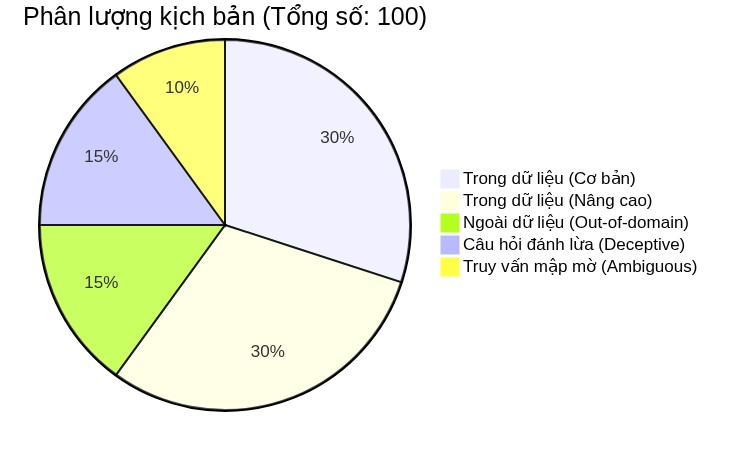
\includegraphics[width=0.85\textwidth]{contents/0/phu_luc/python/bang3.png}

\refstepcounter{figure}
\textbf{Hình \thefigure:} Biểu đồ phân lượng các kịch bản thử nghiệm hệ thống
\label{fig:ti_le_kich_ban_thu_nghiem}
\end{figure}


\begin{longtable}{|l|p{6.5cm}|c|c|}
\caption{Bảng thống kê các kịch bản thử nghiệm hệ thống} \label{tab:thong_ke_chi_tiet} \\
\hline
\makecell[l]{\textbf{Phân loại}\\\textbf{trường hợp}} & \textbf{Câu hỏi} & \makecell{\textbf{Tài liệu}\\\textbf{truy xuất}} & \textbf{Thời gian} \\ \hline
\endfirsthead
\multicolumn{4}{c}{{\bfseries Bảng \thetable{} -- Tiếp theo từ trang trước}} \\
\hline
\makecell[l]{\textbf{Phân loại}\\\textbf{trường hợp}} & \textbf{Câu hỏi} & \makecell{\textbf{Tài liệu}\\\textbf{truy xuất}} & \textbf{Thời gian} \\ \hline
\endhead
\hline
\multicolumn{4}{r}{{Tiếp tục ở trang sau}} \\
\endfoot
\hline
\endlastfoot
\makecell[l]{Trong dữ liệu\\(Cơ bản)} & Thời gian thử việc tối đa đối với người lao động có trình độ đại học là bao lâu? & 44 tài liệu & 64.58s \\ \hline
\makecell[l]{Trong dữ liệu\\(Cơ bản)} & Thời gian thử việc tối đa của lao động có trình độ cao đẳng là bao lâu? & 26 tài liệu & 25.68s \\ \hline
\makecell[l]{Trong dữ liệu\\(Cơ bản)} & Người lao động được nghỉ bao nhiêu ngày phép năm nếu làm đủ 12 tháng trong điều kiện bình thường? & 26 tài liệu & 39.67s \\ \hline
\makecell[l]{Trong dữ liệu\\(Cơ bản)} & Lương thử việc tối thiểu bằng bao nhiêu phần trăm lương của công việc đó? & 22 tài liệu & 14.22s \\ \hline
\makecell[l]{Trong dữ liệu\\(Cơ bản)} & Thời giờ làm việc bình thường không quá bao nhiêu giờ trong một ngày và một tuần? & 0 tài liệu & 1.92s \\ \hline
\makecell[l]{Trong dữ liệu\\(Cơ bản)} & Làm thêm giờ vào ngày nghỉ hằng tuần được trả lương ít nhất bằng bao nhiêu? & 0 tài liệu & 31.91s \\ \hline
\makecell[l]{Trong dữ liệu\\(Cơ bản)} & Làm thêm giờ vào ngày nghỉ lễ, tết, ngày nghỉ có hưởng lương được trả lương ít nhất bằng bao nhiêu? & 0 tài liệu & 30.08s \\ \hline
\makecell[l]{Trong dữ liệu\\(Cơ bản)} & Có bao nhiêu loại hợp đồng lao động theo Bộ luật Lao động hiện hành? & 22 tài liệu & 55.67s \\ \hline
\makecell[l]{Trong dữ liệu\\(Cơ bản)} & Thời gian thử việc đối với công việc cần trình độ chuyên môn kỹ thuật trung cấp là bao lâu? & 23 tài liệu & 13.29s \\ \hline
\makecell[l]{Trong dữ liệu\\(Cơ bản)} & Người lao động làm việc vào ban đêm được trả thêm ít nhất bao nhiêu phần trăm tiền lương? & 0 tài liệu & 29.08s \\ \hline
\makecell[l]{Trong dữ liệu\\(Cơ bản)} & Lao động nữ mang thai từ tháng thứ mấy thì được giảm giờ làm việc hoặc chuyển công việc nhẹ hơn? & 22 tài liệu & 13.99s \\ \hline
\makecell[l]{Trong dữ liệu\\(Cơ bản)} & Người sử dụng lao động có được giữ bản chính giấy tờ tùy thân, văn bằng, chứng chỉ của người lao động không? & 22 tài liệu & 11.91s \\ \hline
\makecell[l]{Trong dữ liệu\\(Cơ bản)} & Tuổi nghỉ hưu của người lao động trong điều kiện lao động bình thường được quy định như thế nào? & 24 tài liệu & 20.74s \\ \hline
\makecell[l]{Trong dữ liệu\\(Cơ bản)} & Người lao động kết hôn được nghỉ bao nhiêu ngày và có được hưởng nguyên lương không? & 22 tài liệu & 13.34s \\ \hline
\makecell[l]{Trong dữ liệu\\(Cơ bản)} & Bố đẻ hoặc mẹ đẻ chết thì người lao động được nghỉ bao nhiêu ngày hưởng nguyên lương? & 22 tài liệu & 13.58s \\ \hline
\makecell[l]{Trong dữ liệu\\(Cơ bản)} & Con kết hôn thì người lao động được nghỉ mấy ngày và có được hưởng lương không? & 25 tài liệu & 64.10s \\ \hline
\makecell[l]{Trong dữ liệu\\(Cơ bản)} & Thời gian nghỉ thai sản của lao động nữ khi sinh con là bao lâu? & 24 tài liệu & 38.21s \\ \hline
\makecell[l]{Trong dữ liệu\\(Cơ bản)} & Khi vợ sinh con, lao động nam đang đóng bảo hiểm xã hội được nghỉ thai sản bao nhiêu ngày? & 48 tài liệu & 123.62s \\ \hline
\makecell[l]{Trong dữ liệu\\(Cơ bản)} & Người lao động làm việc bao lâu cho một người sử dụng lao động thì được tăng thêm 1 ngày phép năm? & 49 tài liệu & 24.51s \\ \hline
\makecell[l]{Trong dữ liệu\\(Cơ bản)} & Hợp đồng thử việc có bắt buộc phải đóng bảo hiểm xã hội không? & 22 tài liệu & 20.96s \\ \hline
\makecell[l]{Trong dữ liệu\\(Cơ bản)} & Người sử dụng lao động phải báo trước bao nhiêu ngày khi đơn phương chấm dứt hợp đồng lao động không xác định thời hạn? & 54 tài liệu & 37.64s \\ \hline
\makecell[l]{Trong dữ liệu\\(Cơ bản)} & Tiền lương trong thời gian nghỉ thai sản của người lao động do cơ quan nào chi trả? & 44 tài liệu & 193.33s \\ \hline
\makecell[l]{Trong dữ liệu\\(Cơ bản)} & Người lao động có được tạm ứng tiền lương khi gặp khó khăn không? & 31 tài liệu & 33.15s \\ \hline
\makecell[l]{Trong dữ liệu\\(Cơ bản)} & Bộ luật Lao động quy định những hình thức xử lý kỷ luật lao động nào? & 75 tài liệu & 50.61s \\ \hline
\makecell[l]{Trong dữ liệu\\(Cơ bản)} & Có được áp dụng nhiều hình thức xử lý kỷ luật lao động đối với một hành vi vi phạm kỷ luật không? & 22 tài liệu & 13.05s \\ \hline
\makecell[l]{Trong dữ liệu\\(Cơ bản)} & Thời hiệu xử lý kỷ luật lao động tối đa là bao lâu? & 22 tài liệu & 12.31s \\ \hline
\makecell[l]{Trong dữ liệu\\(Cơ bản)} & Người lao động bị tạm đình chỉ công việc trong những trường hợp nào? & 31 tài liệu & 21.27s \\ \hline
\makecell[l]{Trong dữ liệu\\(Cơ bản)} & Thời gian tạm đình chỉ công việc tối đa đối với người lao động là bao lâu? & 22 tài liệu & 34.35s \\ \hline
\makecell[l]{Trong dữ liệu\\(Cơ bản)} & Người lao động được nghỉ hưởng nguyên lương vào những ngày lễ, tết nào trong năm? & 29 tài liệu & 55.58s \\ \hline
\makecell[l]{Trong dữ liệu\\(Cơ bản)} & Người sử dụng lao động có phải trả lương cho ngày nghỉ phép hằng năm chưa nghỉ hết không? & 28 tài liệu & 18.42s \\ \hline
\makecell[l]{Trong dữ liệu\\(Nâng cao)} & Cách tính trợ cấp thôi việc cho người lao động làm việc từ 5 năm trở lên? & 22 tài liệu & 33.46s \\ \hline
\makecell[l]{Trong dữ liệu\\(Nâng cao)} & Trường hợp nào người sử dụng lao động được đơn phương chấm dứt hợp đồng lao động mà không cần báo trước? & 25 tài liệu & 62.60s \\ \hline
\makecell[l]{Trong dữ liệu\\(Nâng cao)} & Trợ cấp mất việc làm được tính và chi trả cho người lao động như thế nào? & 22 tài liệu & 29.90s \\ \hline
\makecell[l]{Trong dữ liệu\\(Nâng cao)} & Lao động nữ nuôi con dưới 12 tháng tuổi được hưởng những quyền lợi gì về thời giờ làm việc và nghỉ ngơi? & 46 tài liệu & 139.00s \\ \hline
\makecell[l]{Trong dữ liệu\\(Nâng cao)} & Người lao động đơn phương chấm dứt hợp đồng lao động trái pháp luật thì phải bồi thường những khoản nào? & 30 tài liệu & 21.09s \\ \hline
\makecell[l]{Trong dữ liệu\\(Nâng cao)} & Doanh nghiệp có được quyền sa thải người lao động tự ý bỏ việc 5 ngày cộng dồn trong 30 ngày không? & 22 tài liệu & 86.90s \\ \hline
\makecell[l]{Trong dữ liệu\\(Nâng cao)} & Quy trình xử lý kỷ luật sa thải người lao động cần tuân thủ những bước nào để hợp pháp? & 51 tài liệu & 181.88s \\ \hline
\makecell[l]{Trong dữ liệu\\(Nâng cao)} & Nếu doanh nghiệp đơn phương chấm dứt hợp đồng lao động trái pháp luật thì phải bồi thường những khoản nào cho người lao động? & 46 tài liệu & 82.01s \\ \hline
\makecell[l]{Trong dữ liệu\\(Nâng cao)} & Người lao động làm công việc nặng nhọc, độc hại, nguy hiểm được nghỉ bao nhiêu ngày phép năm? & 51 tài liệu & 38.91s \\ \hline
\makecell[l]{Trong dữ liệu\\(Nâng cao)} & Cách tính tiền lương làm thêm giờ vào ban đêm của ngày nghỉ lễ, tết thế nào? & 0 tài liệu & 224.41s \\ \hline
\makecell[l]{Trong dữ liệu\\(Nâng cao)} & Người sử dụng lao động có được tự ý khấu trừ lương của người lao động để bồi thường thiệt hại dụng cụ bị hư hỏng không? & 22 tài liệu & 63.24s \\ \hline
\makecell[l]{Trong dữ liệu\\(Nâng cao)} & Hợp đồng lao động đương nhiên chấm dứt trong những trường hợp nào? & 32 tài liệu & 146.65s \\ \hline
\makecell[l]{Trong dữ liệu\\(Nâng cao)} & Khi chuyển người lao động sang làm công việc khác so với hợp đồng lao động, doanh nghiệp cần tuân thủ điều kiện gì? & 26 tài liệu & 53.27s \\ \hline
\makecell[l]{Trong dữ liệu\\(Nâng cao)} & Tiền lương của người lao động trong thời gian ngừng việc do lỗi của người sử dụng lao động được tính thế nào? & 22 tài liệu & 23.55s \\ \hline
\makecell[l]{Trong dữ liệu\\(Nâng cao)} & Tiền lương ngừng việc do sự cố điện, nước hoặc thiên tai, dịch bệnh được thỏa thuận như thế nào? & 23 tài liệu & 21.71s \\ \hline
\makecell[l]{Trong dữ liệu\\(Nâng cao)} & Doanh nghiệp có bắt buộc phải thưởng Tết hay lương tháng 13 cho người lao động không? & 22 tài liệu & 191.65s \\ \hline
\makecell[l]{Trong dữ liệu\\(Nâng cao)} & Thỏa ước lao động tập thể là gì và khi nào nó chính thức có hiệu lực? & 22 tài liệu & 19.07s \\ \hline
\makecell[l]{Trong dữ liệu\\(Nâng cao)} & Trình tự, thủ tục giải quyết tranh chấp lao động cá nhân tại Hòa giải viên lao động diễn ra thế nào? & 22 tài liệu & 236.71s \\ \hline
\makecell[l]{Trong dữ liệu\\(Nâng cao)} & Người lao động nước ngoài làm việc tại Việt Nam bắt buộc phải có giấy phép lao động trong trường hợp nào? & 0 tài liệu & 900.35s \\ \hline
\makecell[l]{Trong dữ liệu\\(Nâng cao)} & Hợp đồng lao động bị coi là vô hiệu toàn bộ trong những trường hợp cụ thể nào? & 0 tài liệu & 105.30s \\ \hline
\makecell[l]{Trong dữ liệu\\(Nâng cao)} & Thẩm quyền tuyên bố hợp đồng lao động vô hiệu thuộc về cơ quan nào? & 28 tài liệu & 40.30s \\ \hline
\makecell[l]{Trong dữ liệu\\(Nâng cao)} & Tai nạn lao động được định nghĩa thế nào và doanh nghiệp phải bồi thường ra sao nếu có lỗi của người lao động? & 29 tài liệu & 106.23s \\ \hline
\makecell[l]{Trong dữ liệu\\(Nâng cao)} & Mức bồi thường tai nạn lao động của doanh nghiệp khi lỗi hoàn toàn thuộc về người sử dụng lao động? & 44 tài liệu & 26.37s \\ \hline
\makecell[l]{Trong dữ liệu\\(Nâng cao)} & Chi phí khám và điều trị tai nạn lao động cho người lao động do ai chi trả? & 22 tài liệu & 28.74s \\ \hline
\makecell[l]{Trong dữ liệu\\(Nâng cao)} & Doanh nghiệp có được ký hợp đồng lao động xác định thời hạn nhiều lần với người lao động cao tuổi không? & 31 tài liệu & 36.75s \\ \hline
\makecell[l]{Trong dữ liệu\\(Nâng cao)} & Khi nào người lao động có quyền từ chối làm thêm giờ mà không bị coi là vi phạm kỷ luật lao động? & 22 tài liệu & 11.06s \\ \hline
\makecell[l]{Trong dữ liệu\\(Nâng cao)} & Mức đóng bảo hiểm xã hội, bảo hiểm y tế, bảo hiểm thất nghiệp bắt buộc của người lao động hiện nay là bao nhiêu? & 48 tài liệu & 23.99s \\ \hline
\makecell[l]{Trong dữ liệu\\(Nâng cao)} & Người lao động bị ốm đau dài ngày được hưởng chế độ bảo hiểm xã hội như thế nào? & 51 tài liệu & 51.58s \\ \hline
\makecell[l]{Trong dữ liệu\\(Nâng cao)} & Doanh nghiệp thay đổi cơ cấu, công nghệ ảnh hưởng đến việc làm của nhiều người lao động thì phải lập phương án gì? & 22 tài liệu & 14.31s \\ \hline
\makecell[l]{Trong dữ liệu\\(Nâng cao)} & Quyền lợi ưu tiên thanh toán của người lao động khi doanh nghiệp bị phá sản hoặc giải thể là gì? & 47 tài liệu & 119.56s \\ \hline
\makecell[l]{Ngoài dữ liệu\\(Out-of-domain)} & Công thức tính lực hấp dẫn trong vật lý lượng tử là gì? & 0 tài liệu & 3.44s \\ \hline
\makecell[l]{Ngoài dữ liệu\\(Out-of-domain)} & Cách nấu món phở bò truyền thống của Hà Nội ngon chuẩn vị? & 0 tài liệu & 6.09s \\ \hline
\makecell[l]{Ngoài dữ liệu\\(Out-of-domain)} & Thủ đô của nước Úc là thành phố nào? & 0 tài liệu & 1.84s \\ \hline
\makecell[l]{Ngoài dữ liệu\\(Out-of-domain)} & Làm sao để viết một chương trình Python kết nối với CSDL MySQL? & 0 tài liệu & 7.68s \\ \hline
\makecell[l]{Ngoài dữ liệu\\(Out-of-domain)} & Tác giả của cuốn tiểu thuyết nổi tiếng 'Số Đỏ' là ai? & 0 tài liệu & 2.05s \\ \hline
\makecell[l]{Ngoài dữ liệu\\(Out-of-domain)} & Giải thích thuyết tương đối rộng của Albert Einstein một cách dễ hiểu? & 0 tài liệu & 4.31s \\ \hline
\makecell[l]{Ngoài dữ liệu\\(Out-of-domain)} & Làm thế nào để tự học đàn guitar tại nhà hiệu quả cho người mới bắt đầu? & 0 tài liệu & 4.87s \\ \hline
\makecell[l]{Ngoài dữ liệu\\(Out-of-domain)} & Các bước để đăng ký tài khoản quảng cáo trên Facebook Business? & 0 tài liệu & 4.46s \\ \hline
\makecell[l]{Ngoài dữ liệu\\(Out-of-domain)} & Tác động của biến đổi khí hậu đối với rạn san hô Great Barrier như thế nào? & 0 tài liệu & 4.11s \\ \hline
\makecell[l]{Ngoài dữ liệu\\(Out-of-domain)} & Điện thoại iPhone đầu tiên được Apple ra mắt vào năm nào? & 0 tài liệu & 1.82s \\ \hline
\makecell[l]{Ngoài dữ liệu\\(Out-of-domain)} & Hệ mặt trời của chúng ta có bao nhiêu hành tinh và tên của chúng? & 0 tài liệu & 2.53s \\ \hline
\makecell[l]{Ngoài dữ liệu\\(Out-of-domain)} & Cách điều trị bệnh cảm cúm thông thường tại nhà an toàn? & 0 tài liệu & 4.51s \\ \hline
\makecell[l]{Ngoài dữ liệu\\(Out-of-domain)} & Làm sao để chụp ảnh phong cảnh đẹp bằng điện thoại di động? & 0 tài liệu & 4.17s \\ \hline
\makecell[l]{Ngoài dữ liệu\\(Out-of-domain)} & Lịch sử hình thành và phát triển của mạng Internet toàn cầu? & 0 tài liệu & 6.03s \\ \hline
\makecell[l]{Ngoài dữ liệu\\(Out-of-domain)} & Những địa điểm du lịch nổi tiếng nhất không thể bỏ qua ở Đà Nẵng? & 0 tài liệu & 4.98s \\ \hline
\makecell[l]{Câu hỏi đánh lừa\\(Deceptive)} & Theo luật mới, sinh viên đi làm thêm không cần đóng thuế thu nhập cá nhân đúng không? & 44 tài liệu & 211.81s \\ \hline
\makecell[l]{Câu hỏi đánh lừa\\(Deceptive)} & Tôi nghe nói luật mới cấm hoàn toàn việc thử việc đối với tất cả các ngành nghề đúng không? & 0 tài liệu & 2.79s \\ \hline
\makecell[l]{Câu hỏi đánh lừa\\(Deceptive)} & Tại sao Bộ luật Lao động lại quy định người lao động tự ý nghỉ việc phải bồi thường cho công ty 100 tháng lương? & 0 tài liệu & 3.40s \\ \hline
\makecell[l]{Câu hỏi đánh lừa\\(Deceptive)} & Có đúng là doanh nghiệp không được phép sa thải nhân viên dù họ tự ý nghỉ việc bao nhiêu ngày đi nữa? & 22 tài liệu & 41.67s \\ \hline
\makecell[l]{Câu hỏi đánh lừa\\(Deceptive)} & Luật lao động mới có quy định tăng số ngày nghỉ phép năm tối thiểu từ 12 ngày lên 50 ngày không? & 0 tài liệu & 1.90s \\ \hline
\makecell[l]{Câu hỏi đánh lừa\\(Deceptive)} & Vì sao người lao động thử việc lại được trả lương gấp đôi lương chính thức theo quy định của pháp luật? & 0 tài liệu & 2.63s \\ \hline
\makecell[l]{Câu hỏi đánh lừa\\(Deceptive)} & Nghe nói người đi làm vào ngày Tết được trả lương gấp 10 lần ngày thường, điều này quy định ở điều mấy? & 48 tài liệu & 38.42s \\ \hline
\makecell[l]{Câu hỏi đánh lừa\\(Deceptive)} & Tại sao luật lại bắt buộc nhân viên nam nghỉ thai sản 6 tháng giống như nhân viên nữ khi vợ sinh con? & 0 tài liệu & 3.54s \\ \hline
\makecell[l]{Câu hỏi đánh lừa\\(Deceptive)} & Có đúng là người sử dụng lao động có quyền thu giữ chứng minh nhân dân của nhân viên để làm tin không? & 30 tài liệu & 19.48s \\ \hline
\makecell[l]{Câu hỏi đánh lừa\\(Deceptive)} & Tôi nghe nói hợp đồng lao động bằng lời nói luôn có giá trị cao hơn hợp đồng bằng văn bản, đúng không? & 64 tài liệu & 66.25s \\ \hline
\makecell[l]{Câu hỏi đánh lừa\\(Deceptive)} & Có phải người lao động dưới 18 tuổi thì hoàn toàn không được phép đi làm bất kỳ công việc nào? & 31 tài liệu & 21.35s \\ \hline
\makecell[l]{Câu hỏi đánh lừa\\(Deceptive)} & Có đúng là tiền lương thử việc chỉ được trả tối đa 10\% lương chính thức của công việc đó không? & 16 tài liệu & 40.63s \\ \hline
\makecell[l]{Câu hỏi đánh lừa\\(Deceptive)} & Tại sao luật quy định doanh nghiệp phải trả lương bằng đô la Mỹ (USD) cho người lao động Việt Nam? & 0 tài liệu & 2.52s \\ \hline
\makecell[l]{Câu hỏi đánh lừa\\(Deceptive)} & Nghe nói người lao động đơn phương chấm dứt hợp đồng đúng luật vẫn phải nộp phạt cho công ty, đúng không? & 22 tài liệu & 16.32s \\ \hline
\makecell[l]{Câu hỏi đánh lừa\\(Deceptive)} & Có đúng là người thử việc không cần phải tuân thủ nội quy lao động của doanh nghiệp? & 0 tài liệu & 3.33s \\ \hline
\makecell[l]{Truy vấn mập mờ\\(Ambiguous)} & Làm sao để đăng ký cái đó? & 0 tài liệu & 2.69s \\ \hline
\makecell[l]{Truy vấn mập mờ\\(Ambiguous)} & Cái đó được tính như thế nào? & 0 tài liệu & 2.12s \\ \hline
\makecell[l]{Truy vấn mập mờ\\(Ambiguous)} & Quy định về thời gian nghỉ? & 22 tài liệu & 13.11s \\ \hline
\makecell[l]{Truy vấn mập mờ\\(Ambiguous)} & Tôi phải làm gì khi bị phạt? & 22 tài liệu & 10.82s \\ \hline
\makecell[l]{Truy vấn mập mờ\\(Ambiguous)} & Khi nào thì được nhận tiền đó? & 0 tài liệu & 2.07s \\ \hline
\makecell[l]{Truy vấn mập mờ\\(Ambiguous)} & Thủ tục nghỉ việc thế nào? & 29 tài liệu & 46.93s \\ \hline
\makecell[l]{Truy vấn mập mờ\\(Ambiguous)} & Làm sao để được giảm giờ làm? & 0 tài liệu & 4.68s \\ \hline
\makecell[l]{Truy vấn mập mờ\\(Ambiguous)} & Công ty có được làm thế không? & 0 tài liệu & 1.86s \\ \hline
\makecell[l]{Truy vấn mập mờ\\(Ambiguous)} & Ký cái hợp đồng đó ở đâu? & 30 tài liệu & 57.60s \\ \hline
\makecell[l]{Truy vấn mập mờ\\(Ambiguous)} & Nghỉ thai sản thì thế nào? & 0 tài liệu & 2.74s \\ \hline
\end{longtable}


% \begin{table}[H]
\centering
\refstepcounter{table}
\textbf{Bảng \thetable:} Bảng thống kê hiệu năng và độ chính xác của hệ thống RAG
\label{tab:hieu_nang_do_chinh_xac}
\vspace{0.5em}
\begin{tabular}{|l|c|c|c|c|}
\hline
\textbf{Nhóm câu hỏi kiểm thử} & \makecell{\textbf{Tổng số}\\\textbf{câu hỏi}} & \makecell{\textbf{Phản hồi}\\\textbf{Đúng (\%)}} & \makecell{\textbf{Phản hồi Sai /}\\\textbf{Ảo giác (\%)}} & \makecell{\textbf{Không trả lời do}\\\textbf{không chắc chắn (\%)}} \\ \hline
Câu hỏi có trong CSDL pháp luật & 60 & 33 (55.0\%) & 12 (20.0\%) & 15 (25.0\%) \\ \hline
Câu hỏi ngoài phạm vi (đời sống, IT...) & 15 & 2 (13.3\%) & 13 (86.7\%) & 0 (0.0\%) \\ \hline
Câu hỏi phức tạp, tối nghĩa & 25 & 13 (52.0\%) & 10 (40.0\%) & 2 (8.0\%) \\ \hline
\textbf{Tổng cộng (Overall)} & \textbf{100} & \textbf{48 (48.0\%)} & \textbf{35 (35.0\%)} & \textbf{17 (17.0\%)} \\ \hline
\end{tabular}
\end{table}

\begin{table}[H]
\centering
\refstepcounter{table}
\textbf{Bảng \thetable:} Bảng thống kê độ chính xác (dùng LLM để đánh giá)
\label{tab:thong_ke_5_kich_ban}
\vspace{0.5em}
\begin{tabular}{|l|c|c|c|c|}
\hline
\makecell[l]{\textbf{Phân loại}\\\textbf{kịch bản}} & \makecell{\textbf{Tổng số}\\\textbf{câu hỏi}} & \makecell{\textbf{Phản hồi}\\\textbf{Đúng (\%)}} & \makecell{\textbf{Phản hồi Sai /}\\\textbf{Ảo giác (\%)}} & \makecell{\textbf{Không trả lời do}\\\textbf{không chắc chắn (\%)}} \\ \hline
\makecell[l]{Trong dữ liệu\\(Cơ bản)} & 30 & 16 (53.3\%) & 7 (23.3\%) & 7 (23.3\%) \\ \hline
\makecell[l]{Trong dữ liệu\\(Nâng cao)} & 30 & 17 (56.7\%) & 5 (16.7\%) & 8 (26.7\%) \\ \hline
\makecell[l]{Ngoài dữ liệu\\(Out-of-domain)} & 15 & 2 (13.3\%) & 13 (86.7\%) & 0 (0.0\%) \\ \hline
\makecell[l]{Câu hỏi đánh lừa\\(Deceptive)} & 15 & 9 (60.0\%) & 6 (40.0\%) & 0 (0.0\%) \\ \hline
\makecell[l]{Truy vấn mập mờ\\(Ambiguous)} & 10 & 4 (40.0\%) & 4 (40.0\%) & 2 (20.0\%) \\ \hline
% \textbf{Tổng cộng (Overall)} & \textbf{100} & \textbf{48 (48.0\%)} & \textbf{35 (35.0\%)} & \textbf{17 (17.0\%)} \\ \hline
\end{tabular}
\end{table}


% \newpage

% \subsection*{Bảng thống kê chi tiết}

% \subsection*{Thống kê về câu hỏi và trả lời}

% \newpage
% ==========================================
% Câu hỏi 1: Thời gian thử việc
% ==========================================
% \vspace{1em}
\noindent\textbf{Câu hỏi:} Thời gian thử việc tối đa đối với người lao động có trình độ đại học là bao lâu? \\
\textbf{Link:} \url{https://20206205.tech/share/e334e566-834a-46b2-ab01-5399eb4ce8e0/b4840dbc}

\begin{figure}[H]
\centering
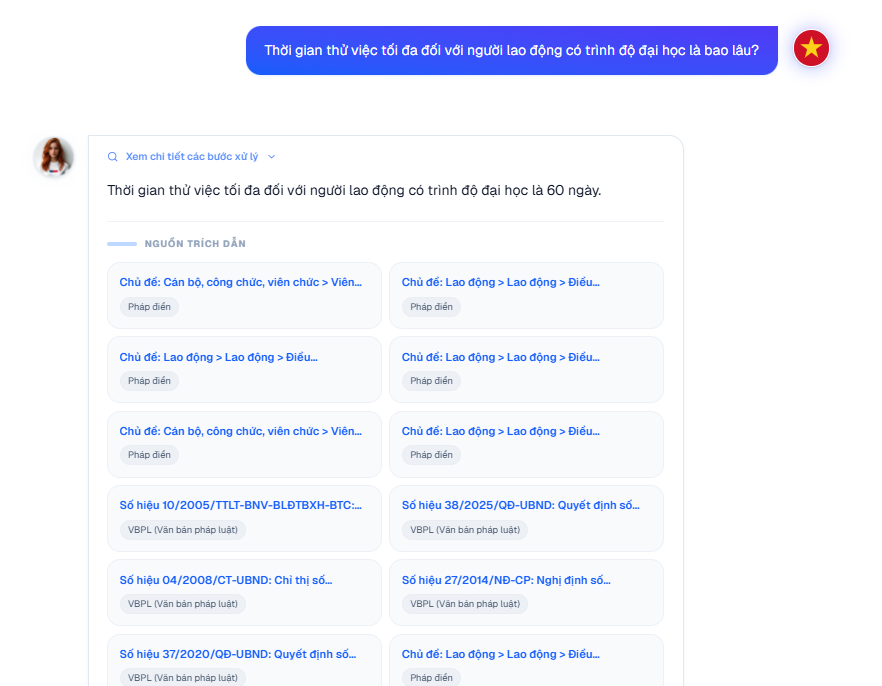
\includegraphics[width=0.65\textwidth]{pictures/chat-ui-image.png}

\refstepcounter{figure}
\textbf{Hình \thefigure:} Giao diện phản hồi câu hỏi về thời gian thử việc của hệ thống
\label{fig:chat_ui_probation}
\end{figure}

\begin{figure}[H]
\centering
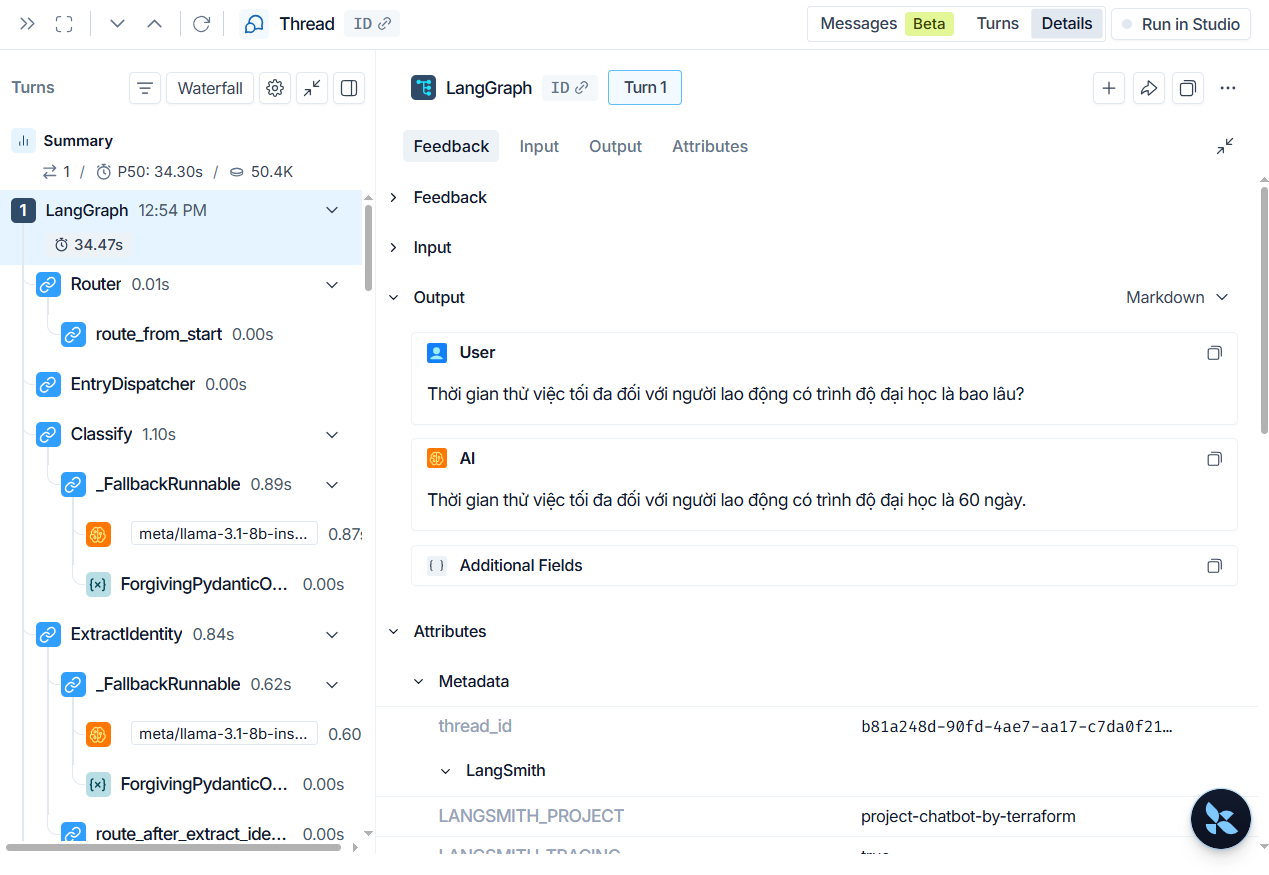
\includegraphics[width=0.65\textwidth]{pictures/langsmith-image-32.png}

\refstepcounter{figure}
\textbf{Hình \thefigure:} Chi tiết LangSmith về thời gian thử việc
\label{fig:langsmith_probation}
\end{figure}

% \newpage
% ==========================================
% Câu hỏi 2: Lực hấp dẫn
% ==========================================
% \vspace{1em}
\noindent\textbf{Câu hỏi:} Công thức tính lực hấp dẫn trong vật lý lượng tử là gì? \\
\textbf{Link:} \url{https://20206205.tech/share/d51942b0-0aff-4ead-88ae-e813c47a9a9c/2f96a259}

\begin{figure}[H]
\centering
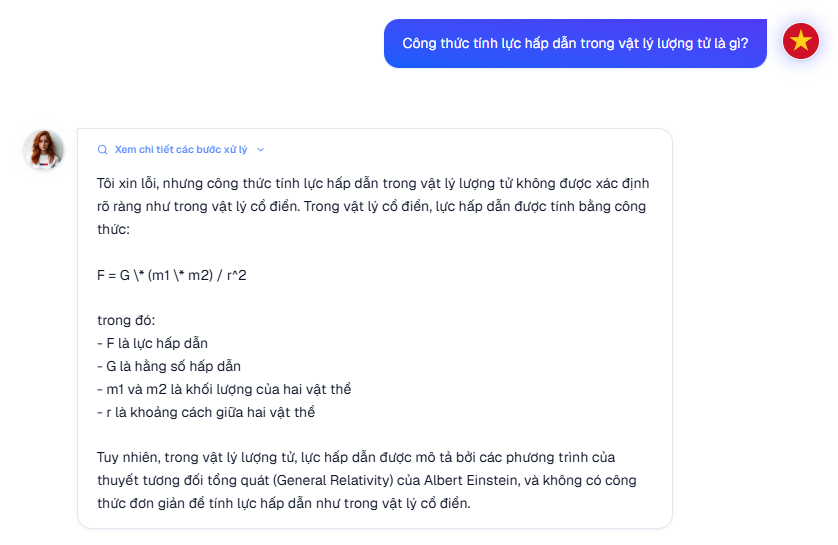
\includegraphics[width=0.65\textwidth]{pictures/chat-ui-image-1.png}

\refstepcounter{figure}
\textbf{Hình \thefigure:} Giao diện phản hồi câu hỏi về lực hấp dẫn trong vật lý lượng tử
\label{fig:chat_ui_gravity}
\end{figure}

\begin{figure}[H]
\centering
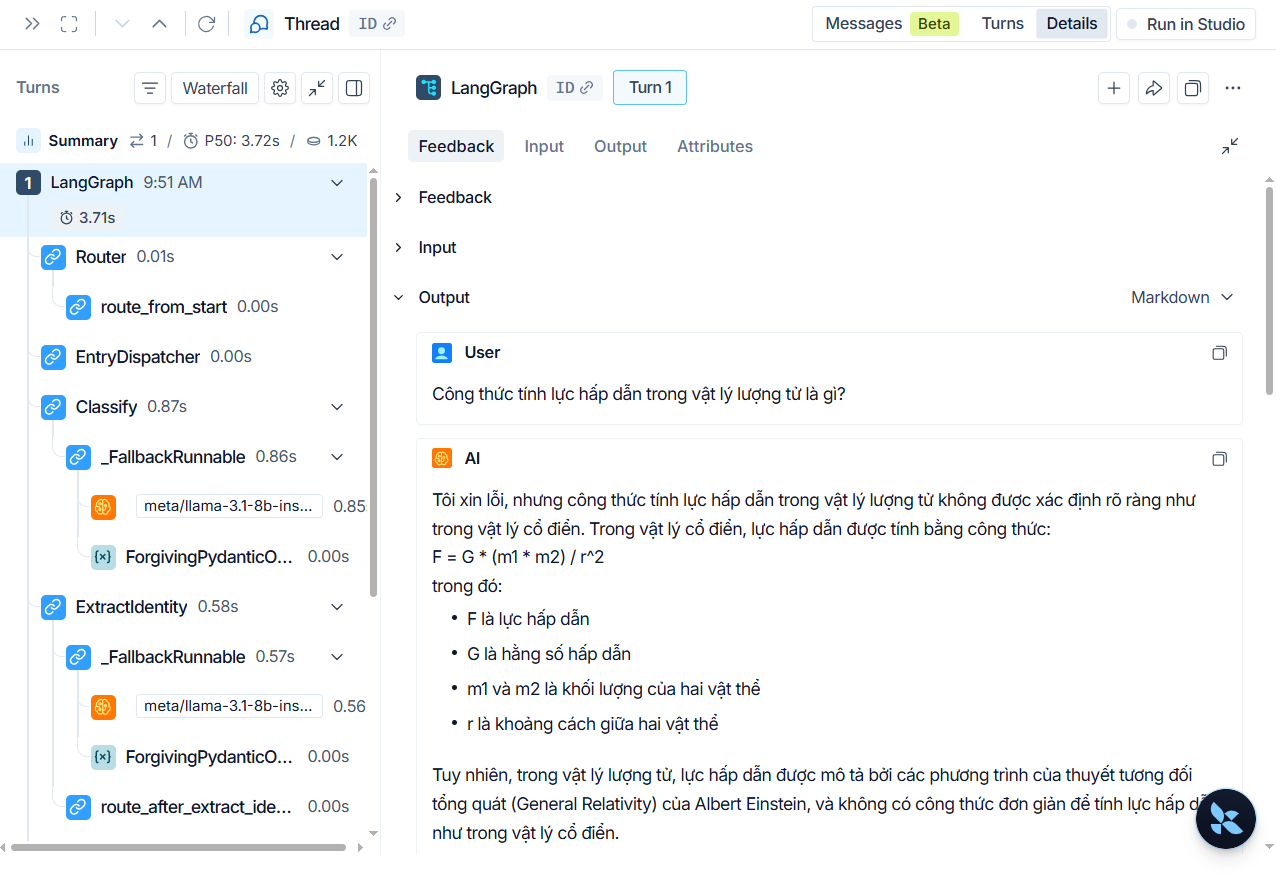
\includegraphics[width=0.65\textwidth]{pictures/langsmith-image-6.png}

\refstepcounter{figure}
\textbf{Hình \thefigure:} Chi tiết LangSmith về lực hấp dẫn
\label{fig:langsmith_gravity}
\end{figure}

% \newpage
% ==========================================
% Câu hỏi 3: Thuế thu nhập cá nhân
% ==========================================
% \vspace{1em}
\noindent\textbf{Câu hỏi:} Theo luật mới, sinh viên đi làm thêm không cần đóng thuế thu nhập cá nhân đúng không? \\
\textbf{Link:} \url{https://20206205.tech/share/0a65a3ff-e2e9-4943-920a-483fab52bfc8/eade4ab7}

\begin{figure}[H]
\centering
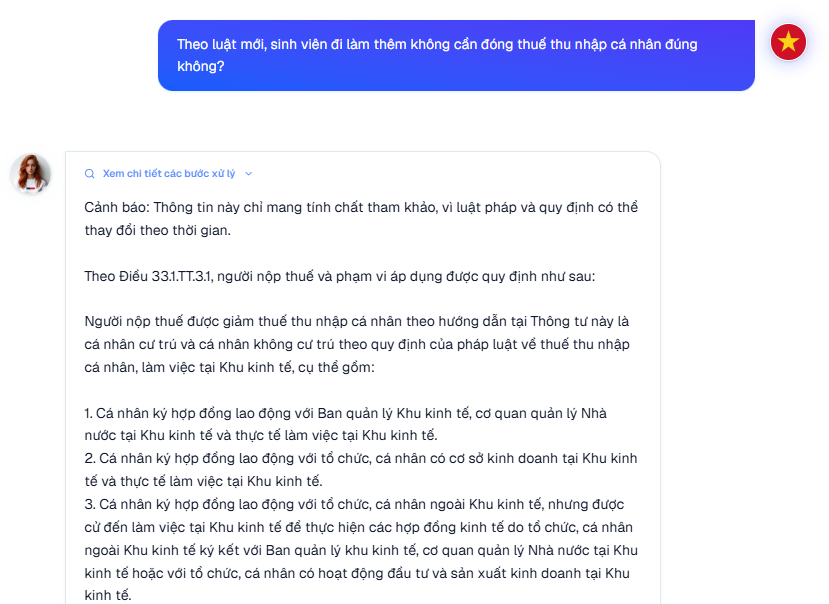
\includegraphics[width=0.65\textwidth]{pictures/chat-ui-image-4.png}

\refstepcounter{figure}
\textbf{Hình \thefigure:} Giao diện phản hồi câu hỏi về thuế thu nhập cá nhân của sinh viên đi làm thêm
\label{fig:chat_ui_tax}
\end{figure}

\begin{figure}[H]
\centering
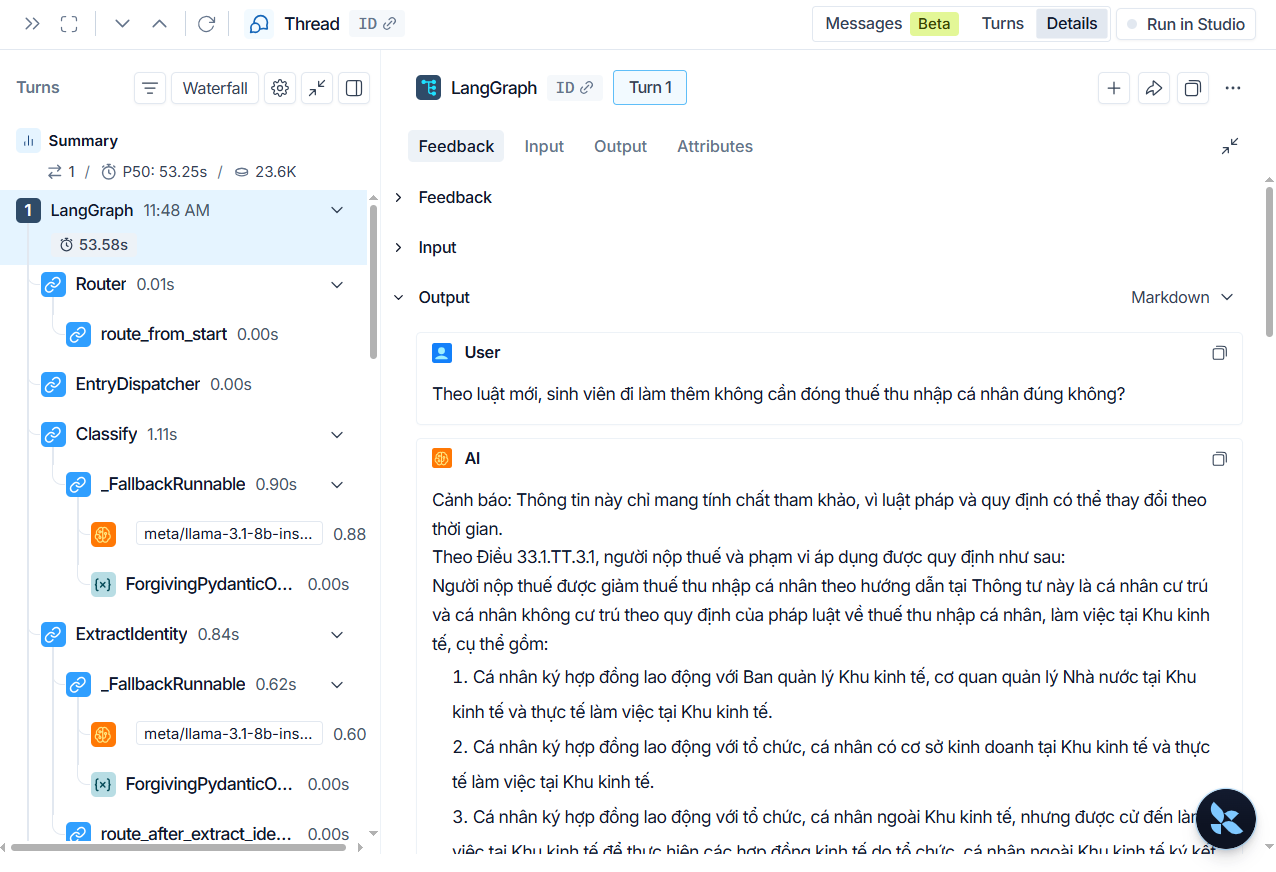
\includegraphics[width=0.65\textwidth]{pictures/langsmith-image-7.png}

\refstepcounter{figure}
\textbf{Hình \thefigure:} Chi tiết LangSmith về thuế thu nhập cá nhân
\label{fig:langsmith_tax}
\end{figure}

% \newpage
% ==========================================
% Câu hỏi 4: Đăng ký thuế
% ==========================================
% \vspace{1em}
\noindent\textbf{Câu hỏi:} Làm sao để đăng ký cái đó? \\
\textbf{Link:} \url{https://20206205.tech/share/8dc3c4e1-b63d-4d70-98f7-a89bfacefadc/2d022228}

\begin{figure}[H]
\centering
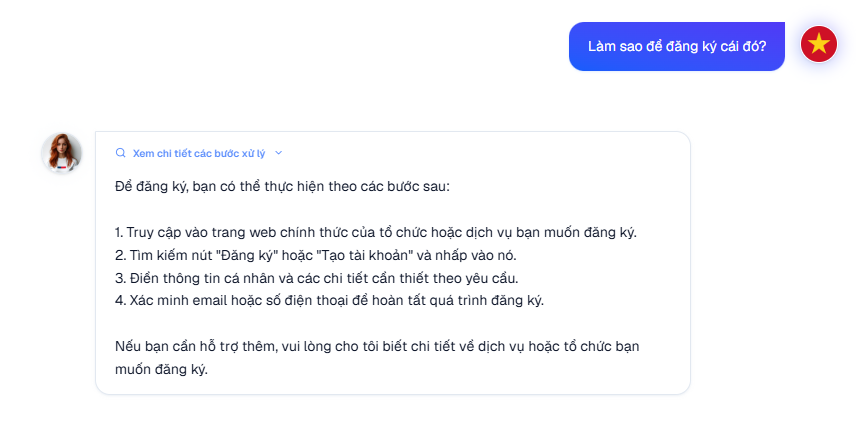
\includegraphics[width=0.9\textwidth]{pictures/chat-ui-image-2.png}

\refstepcounter{figure}
\textbf{Hình \thefigure:} Giao diện phản hồi câu hỏi tiếp nối về cách thức đăng ký
\label{fig:chat_ui_register}
\end{figure}

\begin{figure}[H]
\centering
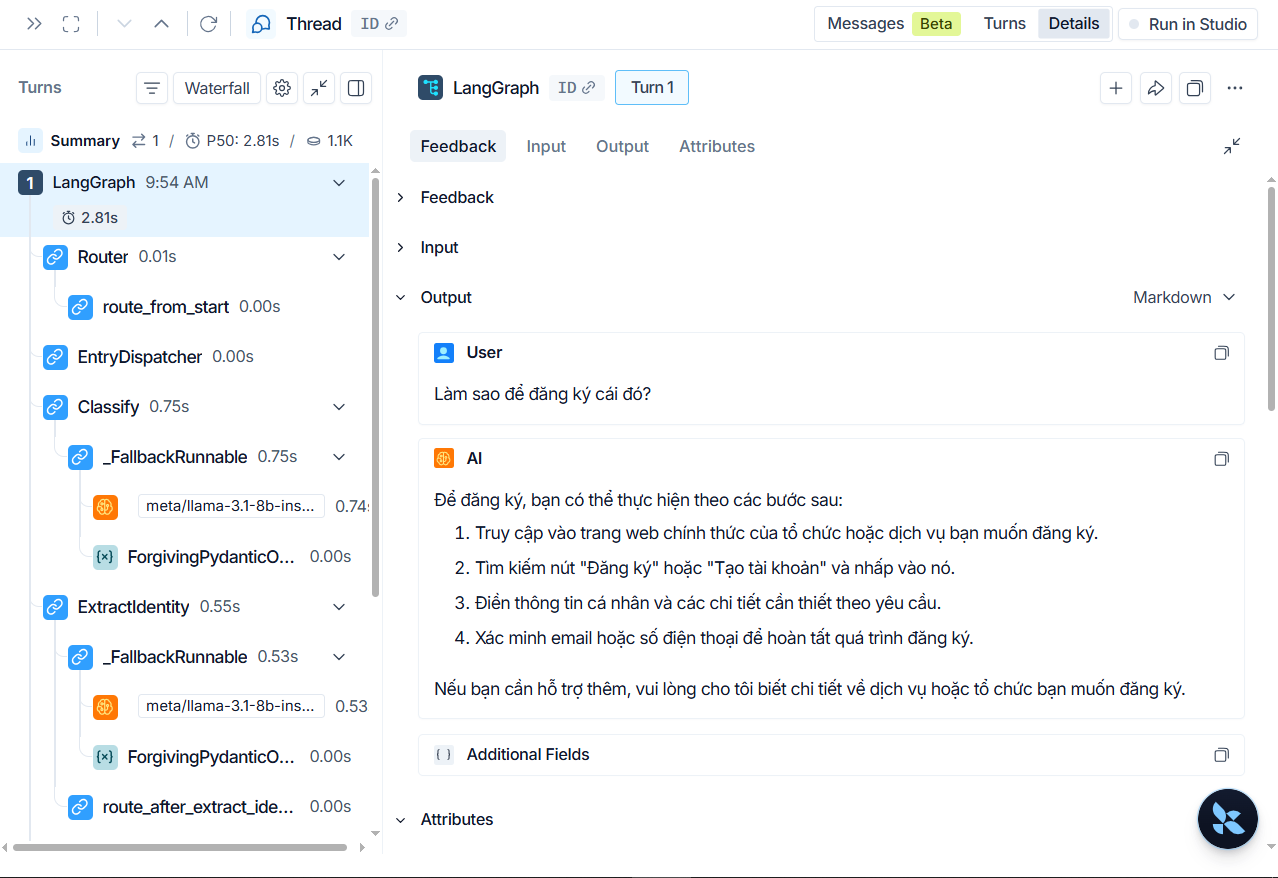
\includegraphics[width=0.65\textwidth]{pictures/langsmith-image-8.png}

\refstepcounter{figure}
\textbf{Hình \thefigure:} Chi tiết LangSmith về cách thức đăng ký
\label{fig:langsmith_register}
\end{figure}

% \newpage
% ==========================================
% Câu hỏi 5: Chấm dứt hợp đồng lao động
% ==========================================
% \vspace{1em}
\noindent\textbf{Câu hỏi:} Người lao động đơn phương chấm dứt hợp đồng lao động xác định thời hạn cần báo trước bao nhiêu ngày? \\
\textbf{Link:} \url{https://20206205.tech/share/80a989ad-6b2e-46b6-84ec-baf843c70e14/0fcaa121}

\begin{figure}[H]
\centering
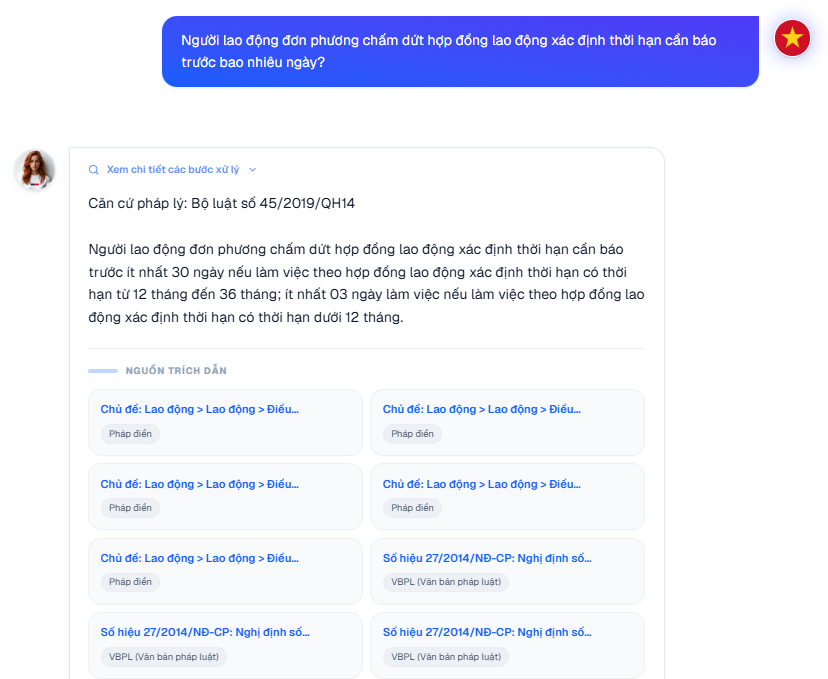
\includegraphics[width=0.65\textwidth]{pictures/chat-ui-image-5.png}

\refstepcounter{figure}
\textbf{Hình \thefigure:} Giao diện phản hồi câu hỏi về chấm dứt hợp đồng lao động
\label{fig:chat_ui_terminate_contract}
\end{figure}

\begin{figure}[H]
\centering
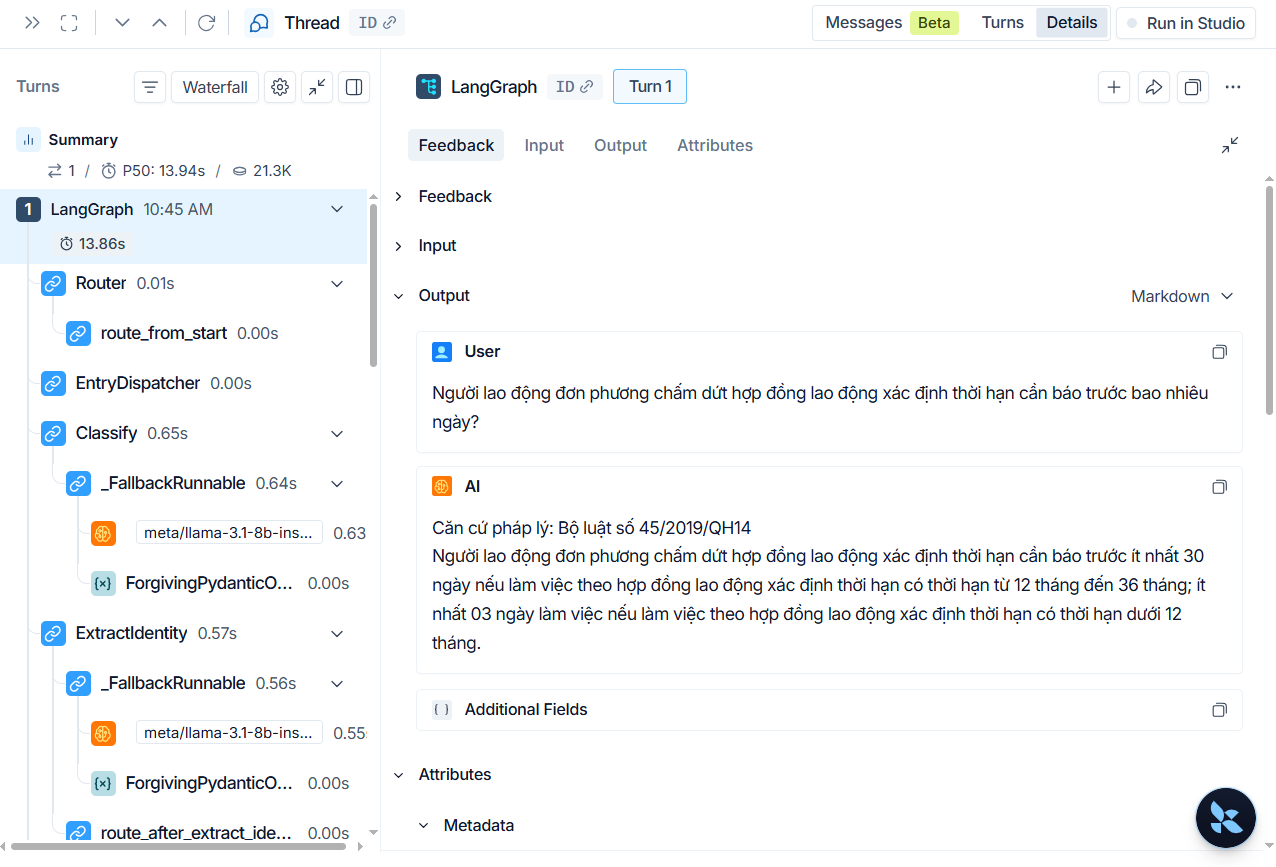
\includegraphics[width=0.65\textwidth]{pictures/langsmith-image-9.png}

\refstepcounter{figure}
\textbf{Hình \thefigure:} Chi tiết LangSmith về chấm dứt hợp đồng lao động
\label{fig:langsmith_terminate_contract}
\end{figure}

\newpage

\vspace*{\fill}
\begin{center}
% Trang này chỉ để trống!
\thispagestyle{empty}
\end{center}
\vspace*{\fill}

\newpage

%%%%%%%%%%%%%%%%%%%%%%%%%%%%%%%%%%%%%%%%%%%%%%%%%%%%%%%
\ifdev
\newpage

{
\color{RedHUST}
Chữ tạm màu đỏ

Dòng thứ hai vẫn có màu đỏ và không bị lỗi ngắt đoạn.
}

\url{https://example.com}

\begin{figure}[H]
\centering

\includegraphics[scale = 0.2]{pictures/LogoHust.png}
\caption{Logo của Đại học Bách Khoa Hà Nội 1}
\end{figure}

\begin{figure}[H]
\centering

\includegraphics[width=0.1\textwidth]{pictures/LogoHust.png}
\caption{Logo của Đại học Bách Khoa Hà Nội 2}
\end{figure}

\begin{itemize}
\item Nội dung mục 1
\item Chấm màu xanh
\end{itemize}

\textit{In nghiêng đoạn văn bản}

\textbf{In đậm đoạn văn bản}

\begin{block}{Ứng dụng trong đồ án}
Nội dung block
\end{block}

\lipsum[1]

\enquote{Đây là văn bản đặc biệt}

\newpage

\fi


\ifdev
% % % % \section{Bài toán nghiệp vụ}

% % % % \begin{frame}{Sự cần thiết}

\begin{itemize}

\item Hệ thống pháp luật rất phức tạp

\item Cá nhân, doanh nghiệp bỏ lỡ cập nhật

\end{itemize}

\begin{figure}[H]
\centering

\includegraphics[width=\linewidth,height=0.55\textheight,keepaspectratio]{pictures/chatbot-tra-cuu-luat-la-gi.jpeg}
\caption[AI hỗ trợ tư vấn pháp luật]{AI hỗ trợ tư vấn pháp luật (Nguồn: \footnotemark)}
\end{figure}
\footnotetext{\url{https://vnptai.io/vi/blog/detail/chatbot-ai-tra-cuu-luat}}

\note{

Hệ thống pháp luật rất phức tạp.

\hrule

Các VBPL có thể thay thế, bổ sung VBPL khác,

hoặc bị hết hiệu lực.

\hrule

Nếu cá nhân, doanh nghiệp bỏ lỡ cập nhật

Và vô tình áp dụng sai luật

\hrule

=> Dẫn đến hậu quả tài chính và rủi ro pháp lý

}

\end{frame}

% hệ thống pháp luật rất phức tạp.

% các văn bản pháp luật có thể thay thế, bổ sung văn bản pháp luật khác

% hoặc bị hết hiệu lực. nếu cá nhân, doanh nghiệp bỏ lỡ cập nhật

% và vô tình áp dụng sai luật. dẫn đến hậu quả tài chính và rủi ro pháp lý


% % % % \begin{frame}{Vai trò và chức năng}
\begin{table}
\centering
\caption{Bảng vai trò và chức năng trong hệ thống} % <-- Lệnh caption được thêm ở đây

% Bây giờ cả hai cột đều có thể dùng 'l' (căn trái) hoặc 'c' (căn giữa)
\begin{tabular}{|l|l|}
\hline
\textbf{Vai trò} & \textbf{Chức năng} \\
\hline

% Dòng 1: Guest
Guest &
\makecell[l]{ % [l] để căn trái các dòng bên trong ô
Giới thiệu, nghe thử giọng nói, xem gói VIP \\
Đăng ký email,
Đăng nhập \textbf{
\textcolor{blue}{G}%
\textcolor{red}{o}%
\textcolor{yellow}{o}%
\textcolor{blue}{g}%
\textcolor{green}{l}%
\textcolor{red}{e}
}
} \\
\hline

% Dòng 2: User
User &
\makecell[l]{
Đăng nhập và quản lý tài khoản, cài đặt \\
Thực hiện trò chuyện, đánh dấu và chia sẻ \\
Mua gói VIP và xem lịch sử
} \\
\hline

% Dòng 3: VIP
VIP &
\makecell[l]{
Suy luận nâng cao\\
Tài liệu cá nhân \\
Sử dụng giọng nói
} \\
\hline

% Dòng 4: Admin
Admin &
\makecell[l]{
Quản lý nhân vật,
gói VIP \\
Báo cáo đường ống dữ liệu
} \\
\hline
\end{tabular}
\end{table}
\end{frame}


% % % % \begin{frame}{Sơ đồ Use Case - Khách vãng lai}
\begin{figure}[H]
\centering
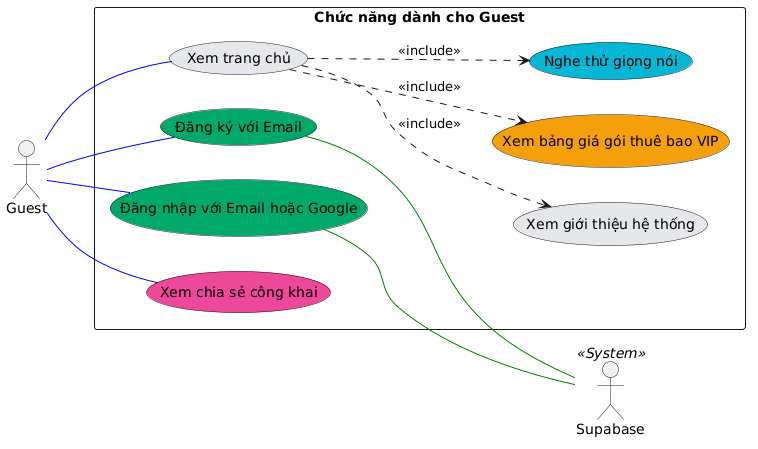
\includegraphics[width=\linewidth,height=0.74\textheight,keepaspectratio]{pictures/UML-UseCase-Guest.png}
\caption{Sơ đồ Use Case chức năng của khách vãng lai}
\end{figure}

\note{

dưới đây là sơ đồ iu cây dành cho người dùng trong hệ thống
\hrule

đầu tiên là khách vãng lai (chưa đăng nhập hệ thống)
\hrule

tiếp theo sơ đồ iu cây dành cho người dùng cơ bản (đã đăng nhập)
\hrule

tiếp theo sơ đồ iu cây dành cho người dùng vip
\hrule

cuối cùng là sơ đồ iu cây dành cho quản trị viên (admin)

}
\end{frame}

% % % % \begin{frame}{Sơ đồ Use Case - Người dùng cơ bản}
\begin{figure}[H]
\centering
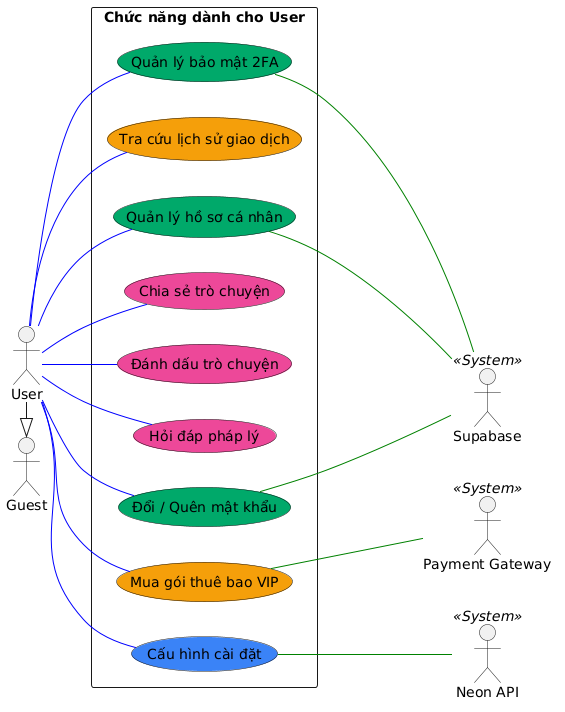
\includegraphics[width=\linewidth,height=0.74\textheight,keepaspectratio]{pictures/UML-UseCase-User.png}
\caption{Sơ đồ Use Case chức năng của người dùng cơ bản}
\end{figure}

\note{

Dưới đây là

Sơ đồ Use Case
chi tiết

dành cho người dùng cơ bản
(đã đăng nhập).

}
\end{frame}

% % % % \begin{frame}{Sơ đồ Use Case - Người dùng VIP}
\begin{figure}[H]
\centering
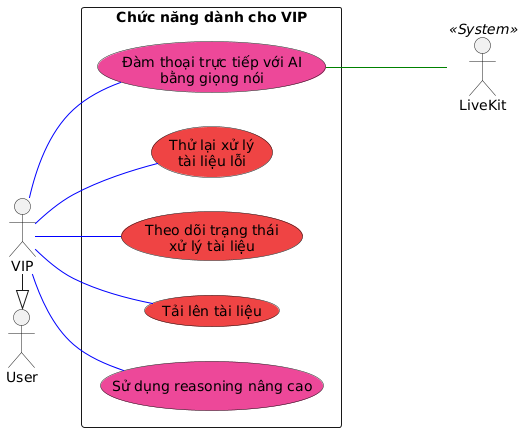
\includegraphics[width=\linewidth,height=0.74\textheight,keepaspectratio]{pictures/UML-UseCase-VIP.png}
\caption{Sơ đồ Use Case chức năng của người dùng VIP}
\end{figure}

\note{

Dưới đây là

Sơ đồ Use Case
chi tiết

dành cho nhóm người dùng VIP.

}
\end{frame}

% % % % \begin{frame}{Sơ đồ Use Case - Quản trị viên}
\begin{figure}[H]
\centering
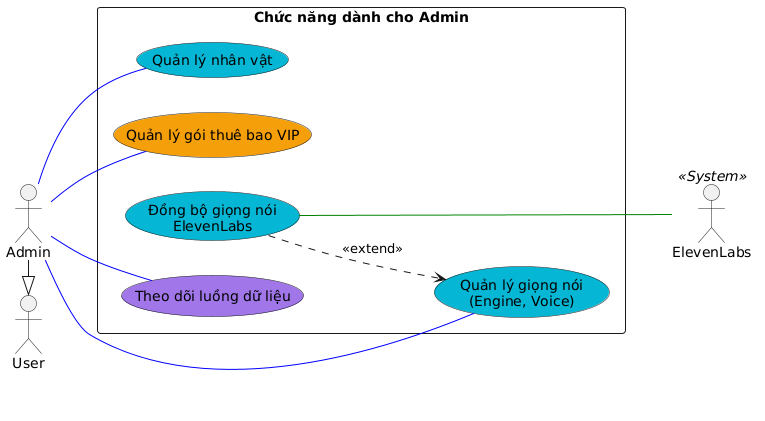
\includegraphics[width=\linewidth,height=0.72\textheight,keepaspectratio]{pictures/UML-UseCase-Admin.png}
\caption{Sơ đồ Use Case chức năng của quản trị viên}
\end{figure}

\note{
Sơ đồ Use Case dành cho quản trị viên (Admin).
Quản trị viên có các quyền hạn cao nhất trong hệ thống bao gồm: quản lý danh sách người dùng, quản lý cấu hình các gói thanh toán VIP, giám sát hệ thống, xem các báo cáo thống kê giao dịch và quản lý các tài liệu pháp luật chung trong CSDL tri thức của hệ thống.
}
\end{frame}


% % % \section{Xây dựng hệ thống AI}
% % % \subsection{Đường ống dữ liệu}

% % % \begin{frame}{Đường ống dữ liệu văn bản pháp luật (VBPL)}
\begin{figure}[H]
\centering
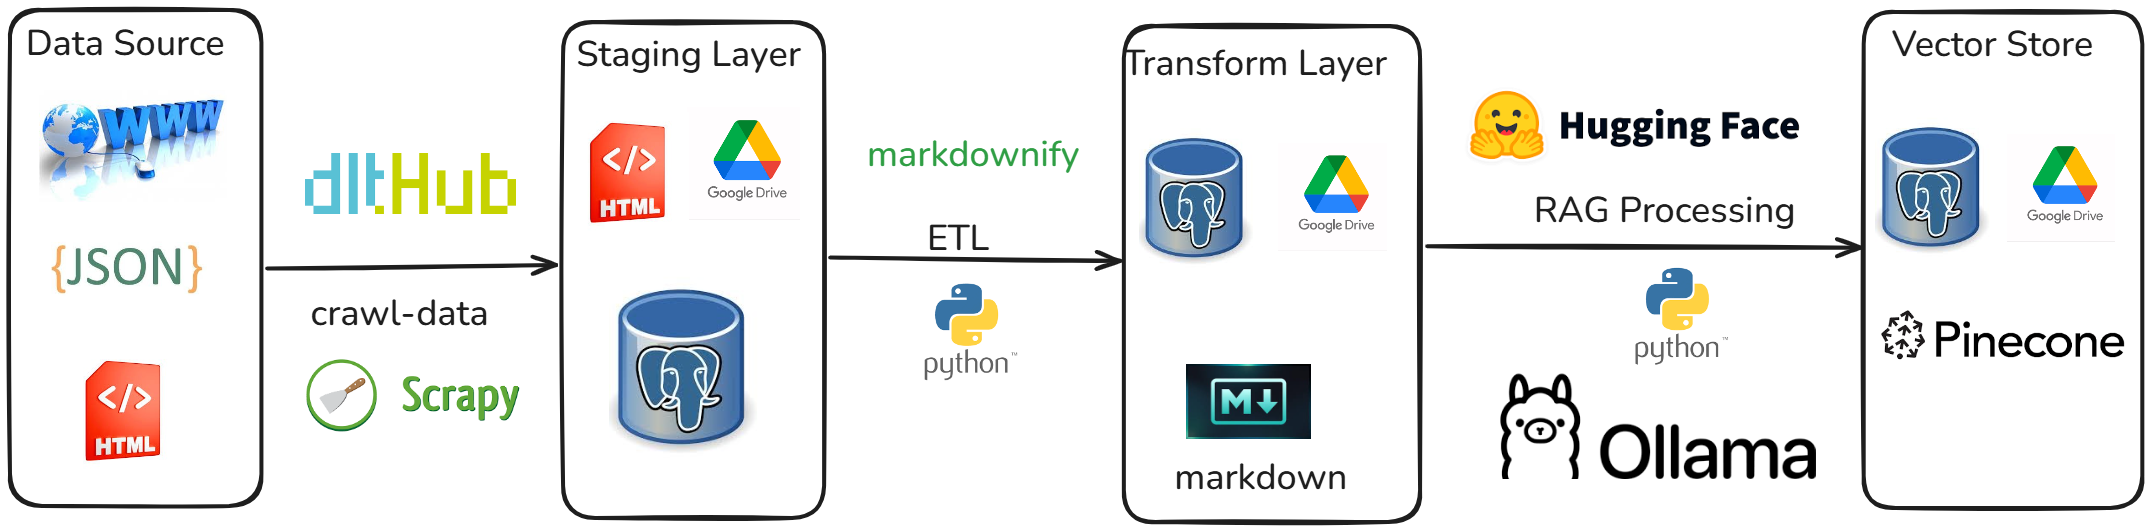
\includegraphics[height=0.55\textheight,width=0.9\textwidth,keepaspectratio]{pictures/Data-Pipeline-VBPL.excalidraw.png}
\caption{Sơ đồ tổng quan luồng dữ liệu văn bản pháp luật mới}
\end{figure}

\note{
Do nguồn dữ liệu Văn bản pháp luật Việt Nam (VBPL) thay đổi cấu trúc trang web và API vào tháng 5/2026, dự án đã xây dựng lại đường ống dữ liệu mới.
Đường ống dữ liệu này tự động hóa quy trình từ thu thập thông tin qua crawler, lưu trữ dữ liệu thô vào PostgreSQL, thực hiện tiền xử lý văn bản pháp luật và cuối cùng là tích hợp vào RAG pipeline để cập nhật CSDL tri thức của trợ lý ảo.
}
\end{frame}

% % % \begin{frame}{Quy trình các bước thu thập dữ liệu văn bản pháp luật}
\begin{figure}[H]
\centering
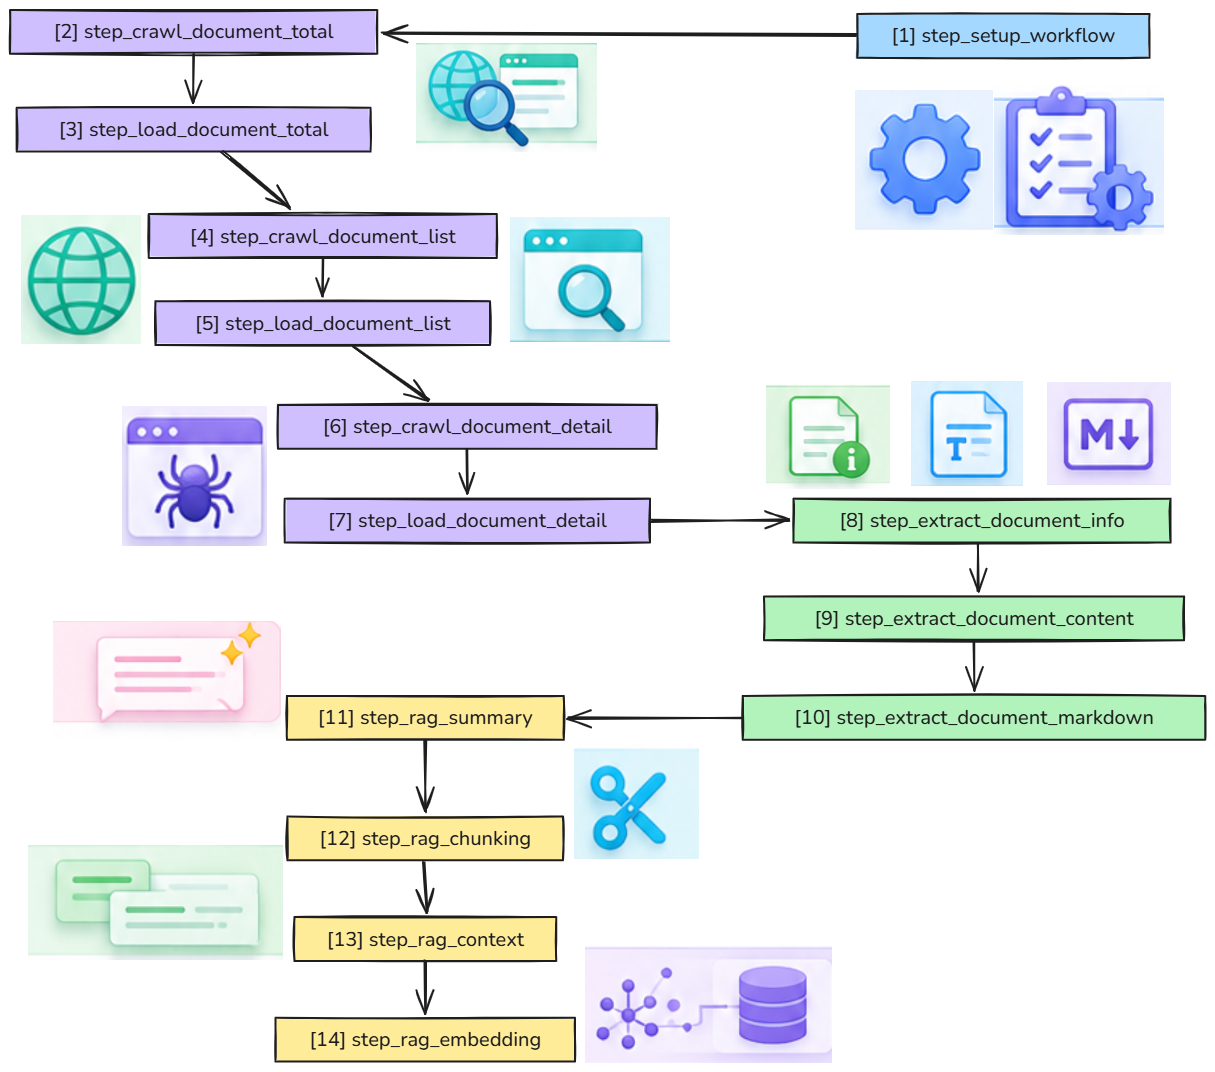
\includegraphics[height=0.55\textheight,width=0.9\textwidth,keepaspectratio]{pictures/step0.excalidraw.png}
\caption{Sơ đồ các bước thực hiện của quy trình cũ}
\end{figure}

\note{
Sơ đồ chi tiết các bước thực hiện trong quy trình cũ của đường ống dữ liệu văn bản pháp luật.
Quy trình được chia thành 3 giai đoạn: Khởi tạo luồng công việc (\texttt{step\_setup\_workflow}), thu thập tổng số lượng tài liệu (\texttt{step\_crawl\_document\_total}), tải nội dung chi tiết và cuối cùng là xử lý định dạng văn bản để chuẩn bị cho việc trích xuất thông tin.
}
\end{frame}

% % % \begin{frame}{Các bước trong đường ống dữ liệu VBPL mới}
\begin{figure}[H]
\centering
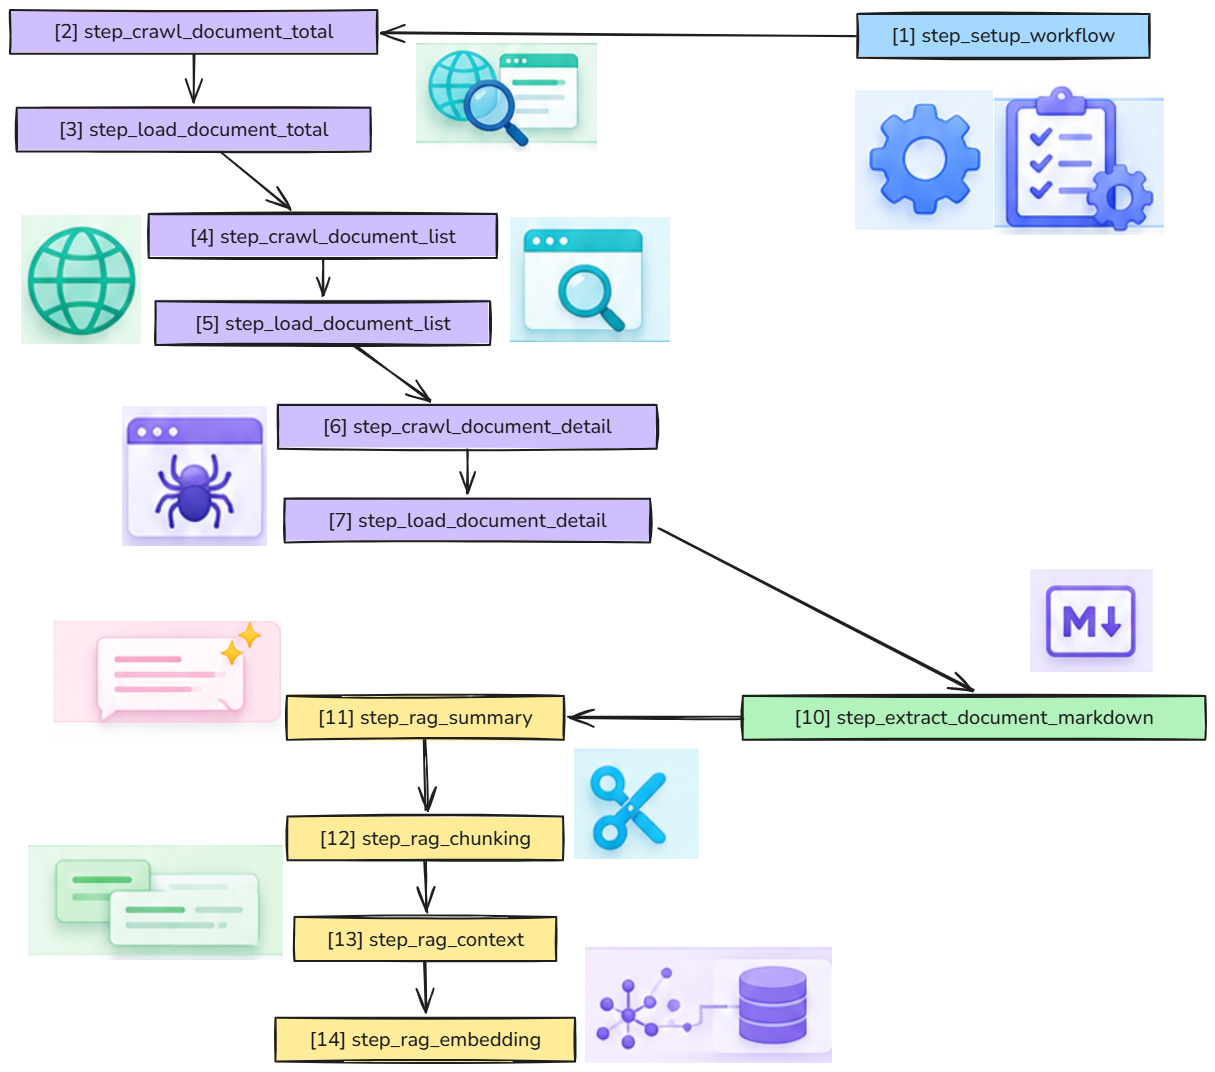
\includegraphics[height=0.7\textheight,width=0.9\textwidth,keepaspectratio]{pictures/step1.excalidraw.png}
\caption{Sơ đồ các bước thực hiện của quy trình mới}
\end{figure}

\note{
do api => bỏ bước

Sơ đồ các bước thực hiện của quy trình mới
}
\end{frame}

% % % \begin{frame}{Đường ống dữ liệu Pháp Điển}
\begin{figure}[H]
\centering
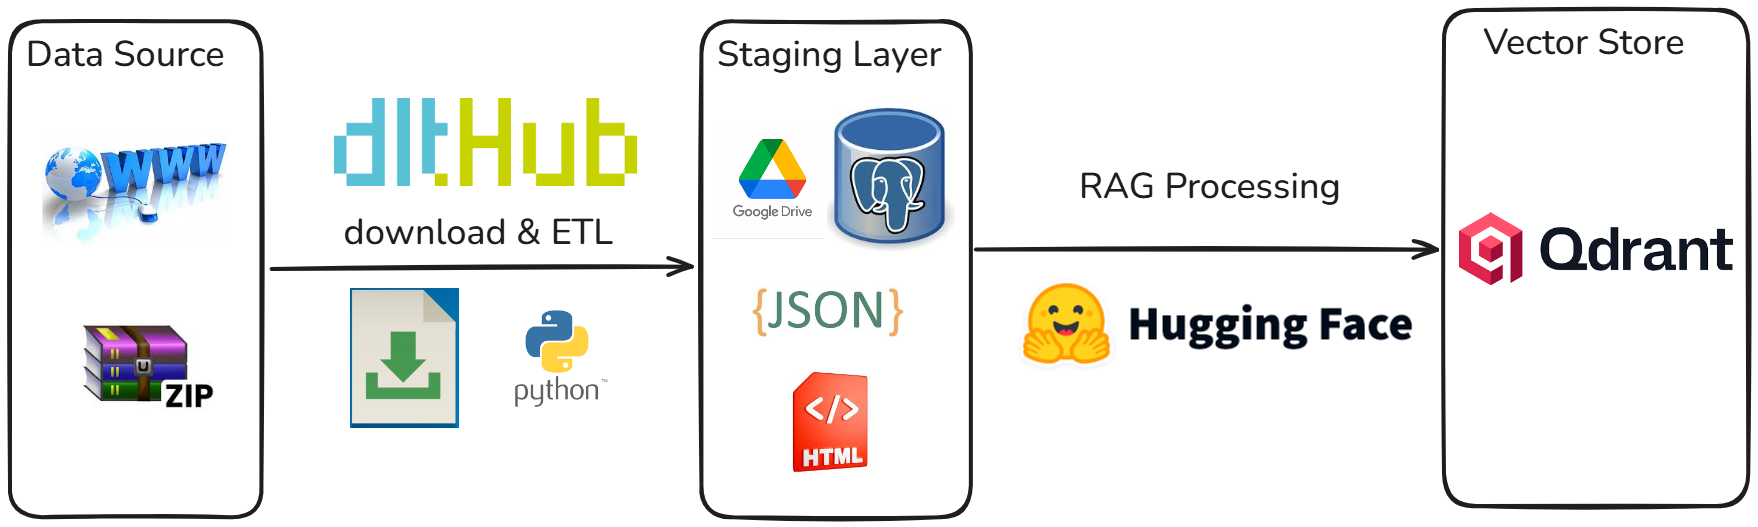
\includegraphics[height=0.55\textheight,width=0.9\textwidth,keepaspectratio]{pictures/Data-Pipeline-PhapDien.excalidraw.png}
\caption{Sơ đồ tổng quan đường ống dữ liệu Pháp Điển}
\end{figure}

\note{
Bên cạnh VBPL, hệ thống còn tích hợp Bộ Pháp Điển Việt Nam. Sơ đồ này mô tả đường ống dữ liệu Pháp Điển.
Dữ liệu Pháp Điển được tải về dưới dạng file nén ZIP từ Cổng thông tin điện tử Pháp Điển, sau đó được giải nén, chuyển đổi cấu trúc cây đề mục sang định dạng JSON, tải lên lưu trữ trên Google Drive và thực hiện vector hóa để lưu vào Vector Database.
}
\end{frame}

% % % \begin{frame}{Các bước trong đường ống dữ liệu Pháp Điển}

\begin{figure}[H]
\centering
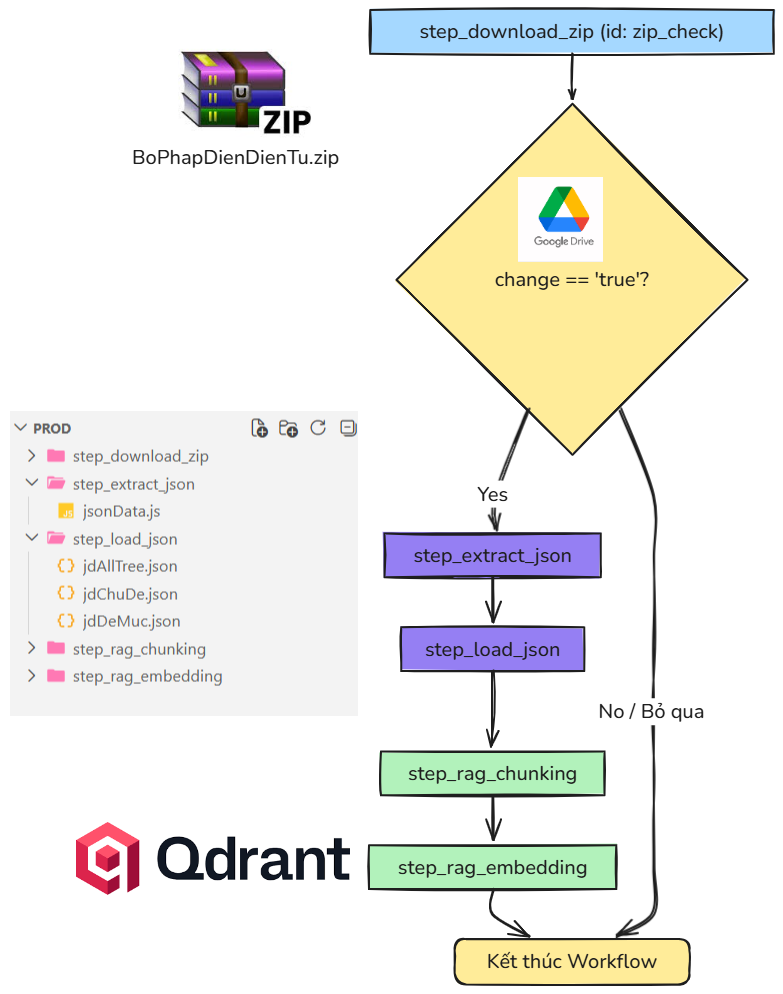
\includegraphics[height=0.7\textheight,width=0.9\textwidth,keepaspectratio]{pictures/step3.excalidraw.png}
\caption{Sơ đồ các bước thực hiện của đường ống dữ liệu Pháp Điển}
\end{figure}

\note{
Sơ đồ mô tả quy trình từng bước của đường ống dữ liệu Pháp Điển.
Quy trình bắt đầu từ việc tải file ZIP tự động (\texttt{step\_download\_zip}), tính toán mã băm MD5 để kiểm tra sự thay đổi dữ liệu so với phiên bản trước, giải nén và trích xuất cấu trúc đề mục ra các file JSON riêng biệt, sau đó chạy các tác vụ phân tích cấu trúc và lưu kết quả vector hóa.
}
\end{frame}


% % % \subsection{Agentic RAG với LangGraph}

% % % \begin{frame}{Kiến trúc Agentic RAG bằng LangGraph}
\begin{figure}[H]
\centering
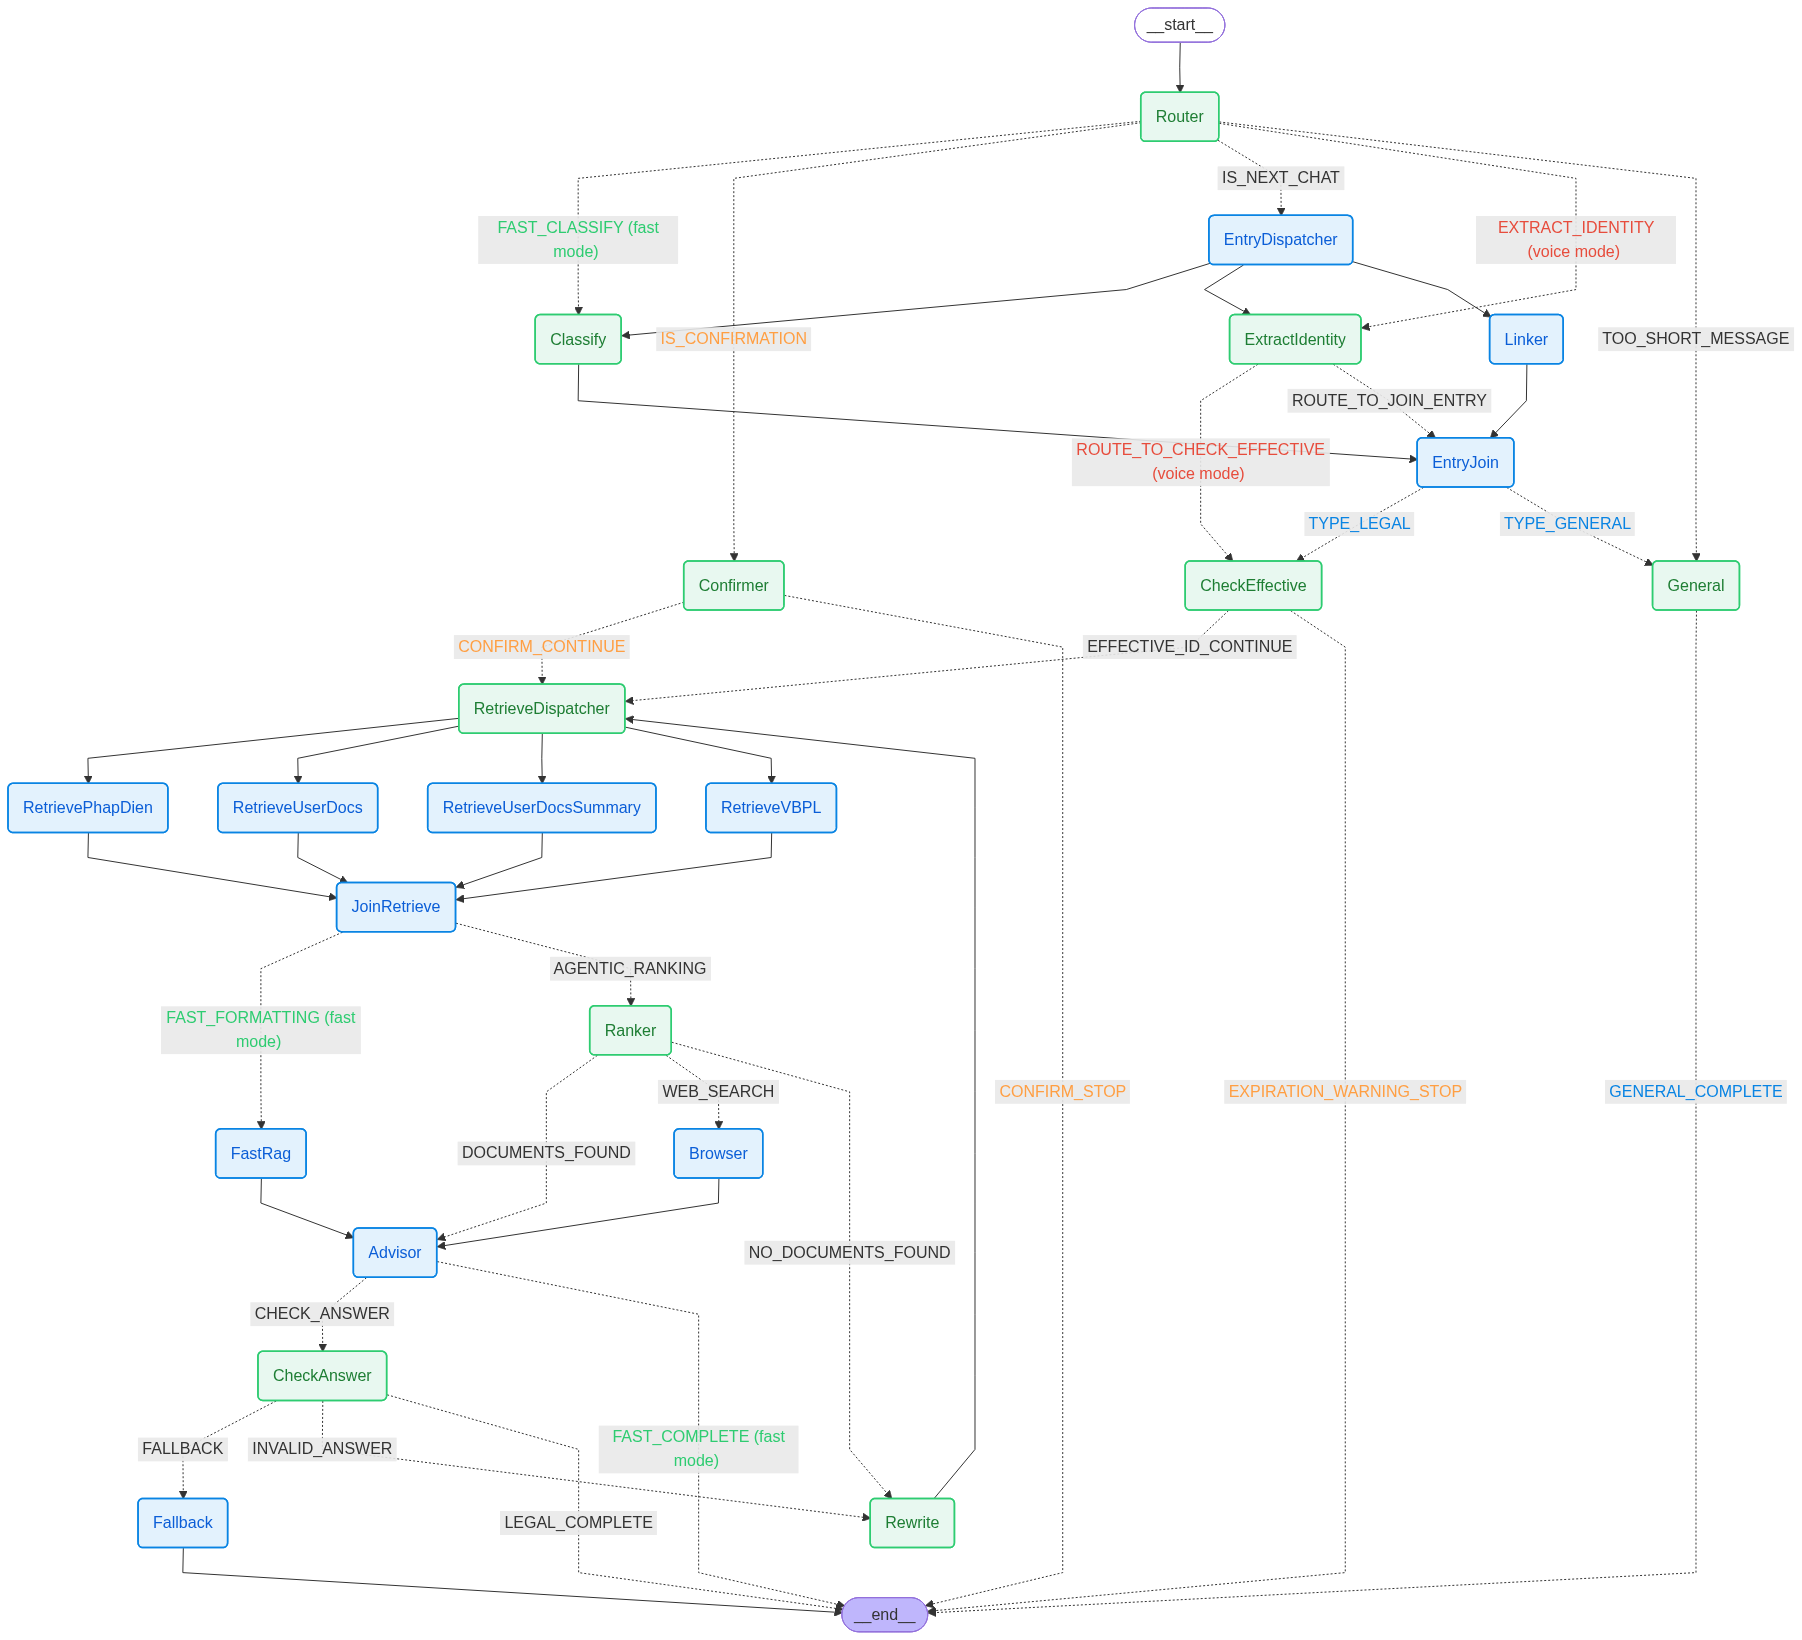
\includegraphics[height=0.55\textheight,width=0.9\textwidth,keepaspectratio]{pictures/rag_diagram.png}
\caption{Sơ đồ LangGraph của dự án}
\end{figure}

\note{
Đây là sơ đồ Agentic RAG của dự án được xây dựng bằng LangGraph. Hệ thống phân chia thông minh giữa mô hình nhỏ cho luồng cơ bản (màu xanh lá) và mô hình lớn cho các tác vụ suy luận phức tạp (màu xanh dương) để tối ưu chi phí và độ trễ.
Mỗi tin nhắn đi qua Router để kiểm tra điều kiện và định tuyến qua các node như rewrite query, retrieve tài liệu và sinh câu trả lời.
}
\end{frame}


% % % \begin{frame}{Tổng quan các dịch vụ}
\begin{figure}[H]
\centering
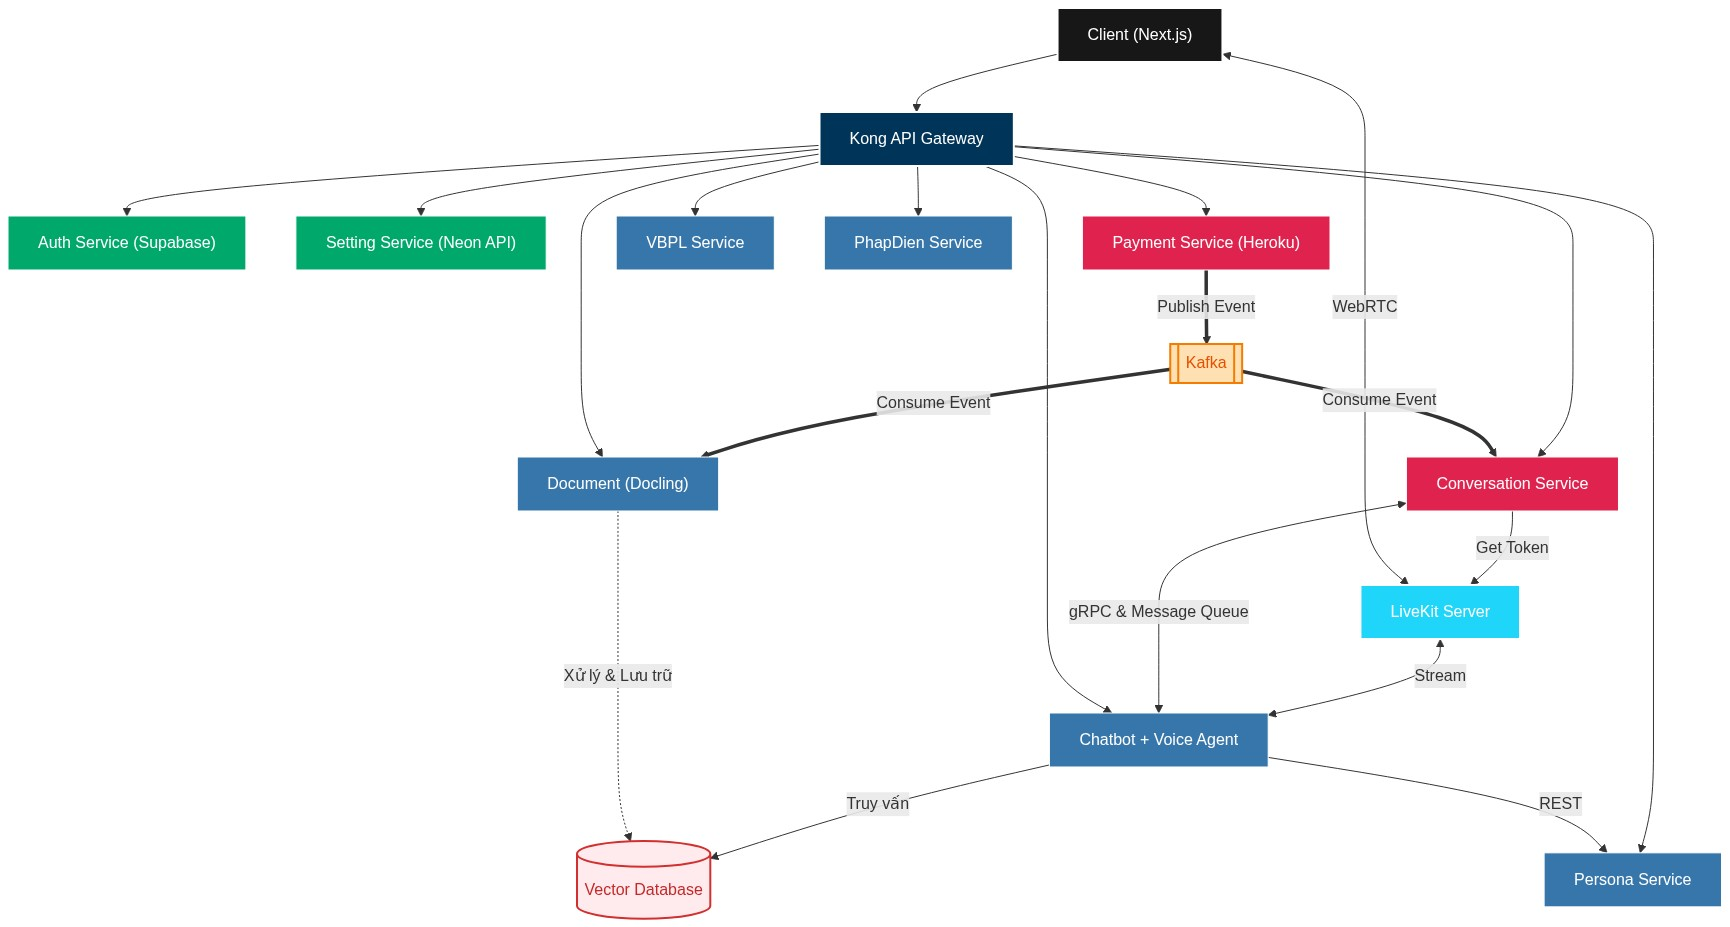
\includegraphics[height=0.7\textheight,width=0.9\textwidth,keepaspectratio]{pictures/MSA.png}
\caption{Tổng quan các dịch vụ của dự án}
\end{figure}

\note{
Sơ đồ tổng quan về kiến trúc các vi dịch vụ được triển khai trong dự án này.
Hệ thống được chia thành nhiều dịch vụ chuyên biệt như: Auth Service (xác thực), Document Service (quản lý tài liệu), Conversation Service (quản lý trò chuyện), Chatbot Service (trí tuệ nhân tạo) và Payment Service (thanh toán). Các dịch vụ này giao tiếp với nhau qua gRPC, REST API hoặc thông điệp bất đồng bộ qua Kafka/RabbitMQ.
}
\end{frame}
% nếu python cash => thanh toán , đăng nhập vẫn không sao

% Nếu các Microservice luôn để xuống service thanh toán


% % \section{Chi tiết các dịch vụ}

% % \begin{frame}{Kiến trúc Dịch vụ Thanh toán (Payment Service)}
\begin{figure}[H]
\centering
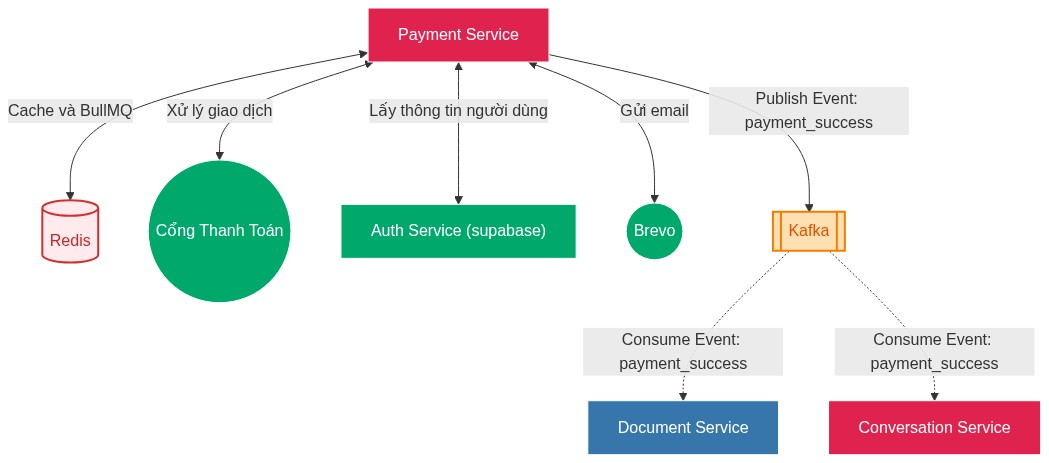
\includegraphics[height=0.7\textheight,width=0.9\textwidth,keepaspectratio]{pictures/payment-kafka-event.png}
\caption{Sơ đồ tổng quan dịch vụ thanh toán}
\end{figure}

\note{
Dịch vụ thanh toán (Payment Service) chịu trách nhiệm quản lý thông tin các gói dịch vụ (Plans), quản lý thuê bao người dùng (Subscriptions) và tích hợp với cổng thanh toán ngoại vi.
Khi người dùng thực hiện thanh toán thành công, dịch vụ này sẽ phát đi sự kiện \texttt{payment\_success} vào hệ thống truyền tin nhắn Kafka để các dịch vụ khác như Chatbot và Document cập nhật quyền VIP cho người dùng.
}
\end{frame}


% % \begin{frame}{Dịch vụ Tài liệu (Document Service)}
\begin{figure}[H]
\centering
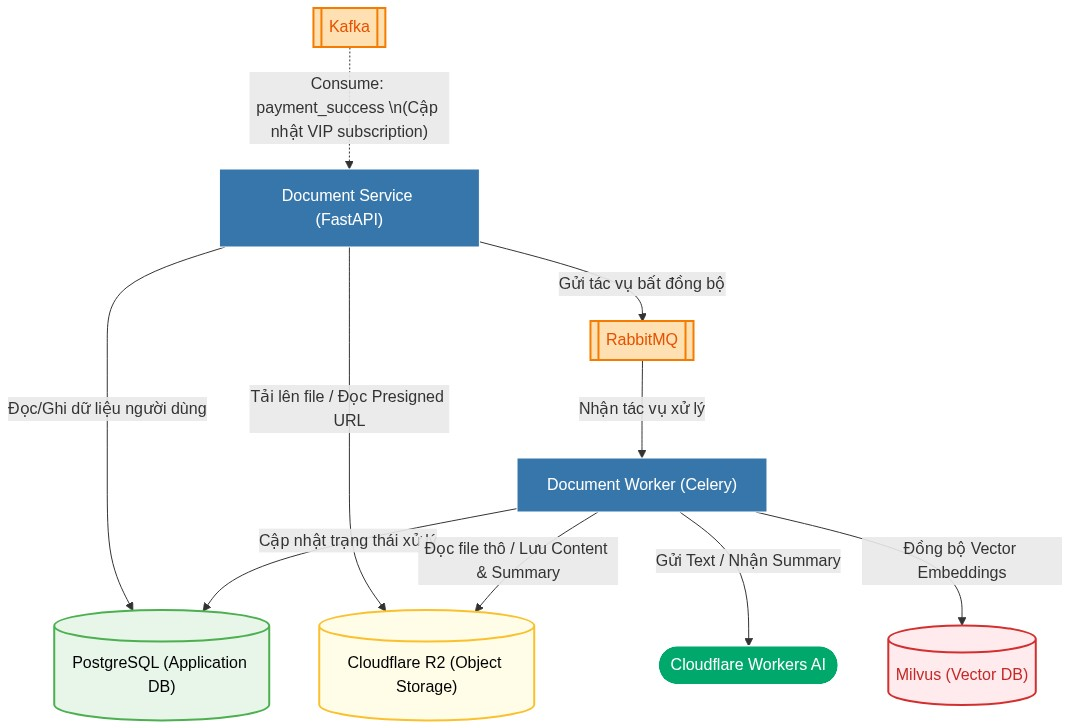
\includegraphics[height=0.7\textheight,width=0.9\textwidth,keepaspectratio]{pictures/document-overview.png}
\caption{Sơ đồ tổng quan dịch vụ văn bản}
\end{figure}

\note{
Dịch vụ tài liệu (Document Service) tiếp nhận, lưu trữ và quản lý tài liệu do người dùng VIP tải lên.
Khi nhận được tệp tin (PDF, DOCX), dịch vụ sẽ gửi yêu cầu xử lý bất đồng bộ thông qua RabbitMQ tới Document Worker. Tài liệu sẽ được trích xuất nội dung sang định dạng Markdown, tự động tóm tắt nội dung chính và tiến hành vector hóa để lưu trữ vào Vector Database Milvus phục vụ cho việc hỏi đáp trên tài liệu.
}
\end{frame}


% % \begin{frame}{Dịch vụ Chatbot và Trò chuyện}
\begin{figure}[H]
\centering
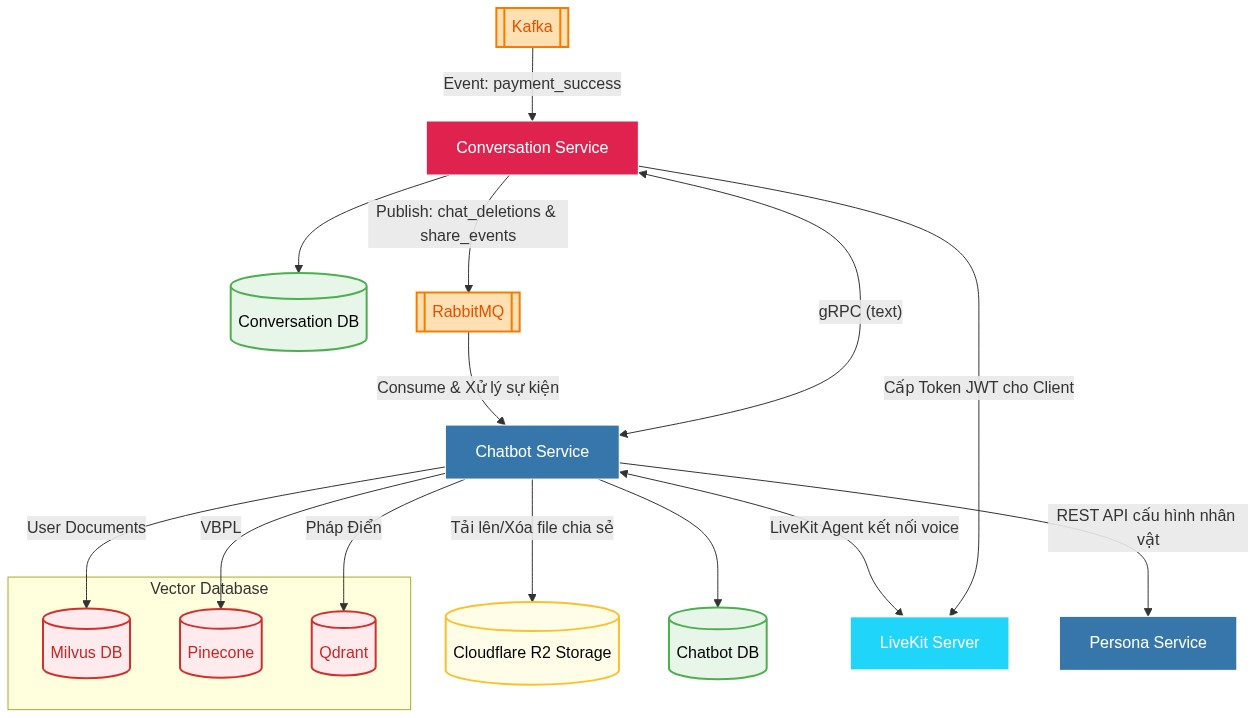
\includegraphics[height=0.7\textheight,width=0.9\textwidth,keepaspectratio]{pictures/conversation-and-chatbot-overview.png}
\caption{Sơ đồ tổng quan dịch vụ trò chuyện và dịch vụ chatbot}
\end{figure}

\note{
Sơ đồ mối quan hệ giữa Dịch vụ trò chuyện (NestJS) và Dịch vụ chatbot (Python).
Dịch vụ trò chuyện chịu trách nhiệm quản lý
trò chuyện của người dùng, lưu trữ lịch sử chat, quản lý thư mục, chia sẻ trò chuyện. Khi có tin nhắn mới, dịch vụ trò chuyện sẽ gửi yêu cầu qua giao thức gRPC hiệu năng cao đến dịch vụ chatbot (Python) để xử lý logic Agentic RAG và trả về câu trả lời dưới dạng stream.
}
\end{frame}


% % \begin{frame}{Kiến trúc tích hợp đàm thoại thời gian thực (Voice Agent)}
\begin{figure}[H]
\centering
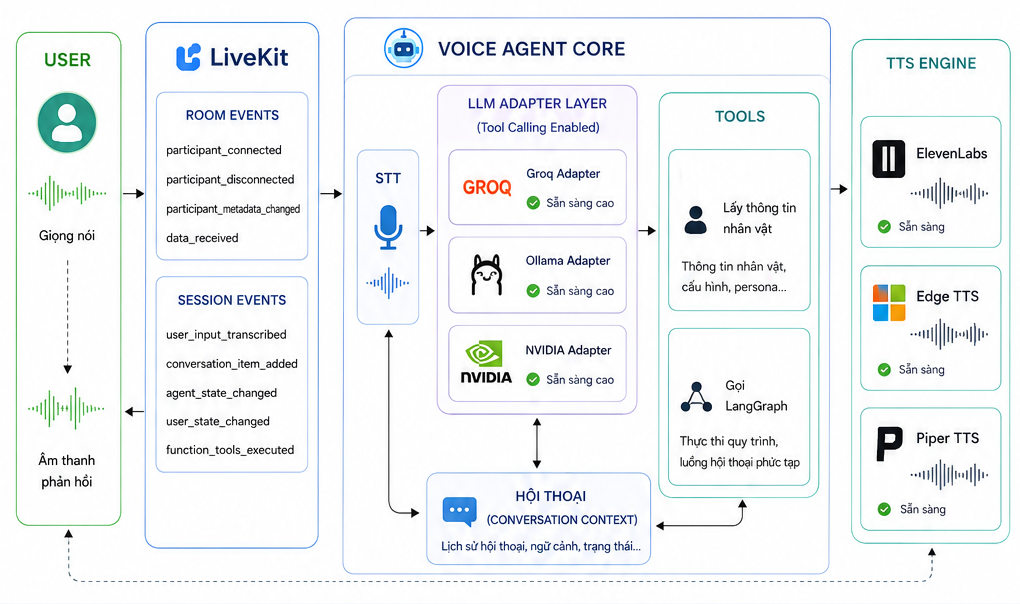
\includegraphics[height=0.7\textheight,width=0.9\textwidth,keepaspectratio]{pictures/voice-livekit-overview.png}
\caption{Sơ đồ tích hợp LiveKit đàm thoại giọng nói}
\end{figure}

\note{
Hệ thống tích hợp máy chủ LiveKit để cung cấp tính năng đàm thoại giọng nói thời gian thực với trợ lý ảo.
Khi người dùng kết nối, Voice Agent hoạt động như một LiveKit Agent, chủ động kết nối và trao đổi âm thanh hai chiều thông qua giao thức WebRTC. Voice Agent tích hợp các mô hình VAD (phát hiện giọng nói), STT (chuyển giọng nói thành văn bản), LLM (suy luận phản hồi) và TTS (chuyển văn bản thành giọng nói) với độ trễ cực thấp.
}
\end{frame}


% \ifdev
% \begin{frame}
\frametitle{}
\maketitle
\end{frame}

\begin{frame}{Cảm ơn}
\centering
\Huge{Thanks for listening!}
\end{frame}

\begin{frame}{Cảm ơn}
\centering
\Huge{Thanks for listening!}
\end{frame}

% \fi

\section{Các công nghệ khác}

\input{contents/Quy_trinh_tu_dong_hoa_CICD_bang_GitHub_Actions}
\begin{frame}{Quản lý Hạ tầng dưới dạng mã}
\begin{figure}[H]
\centering
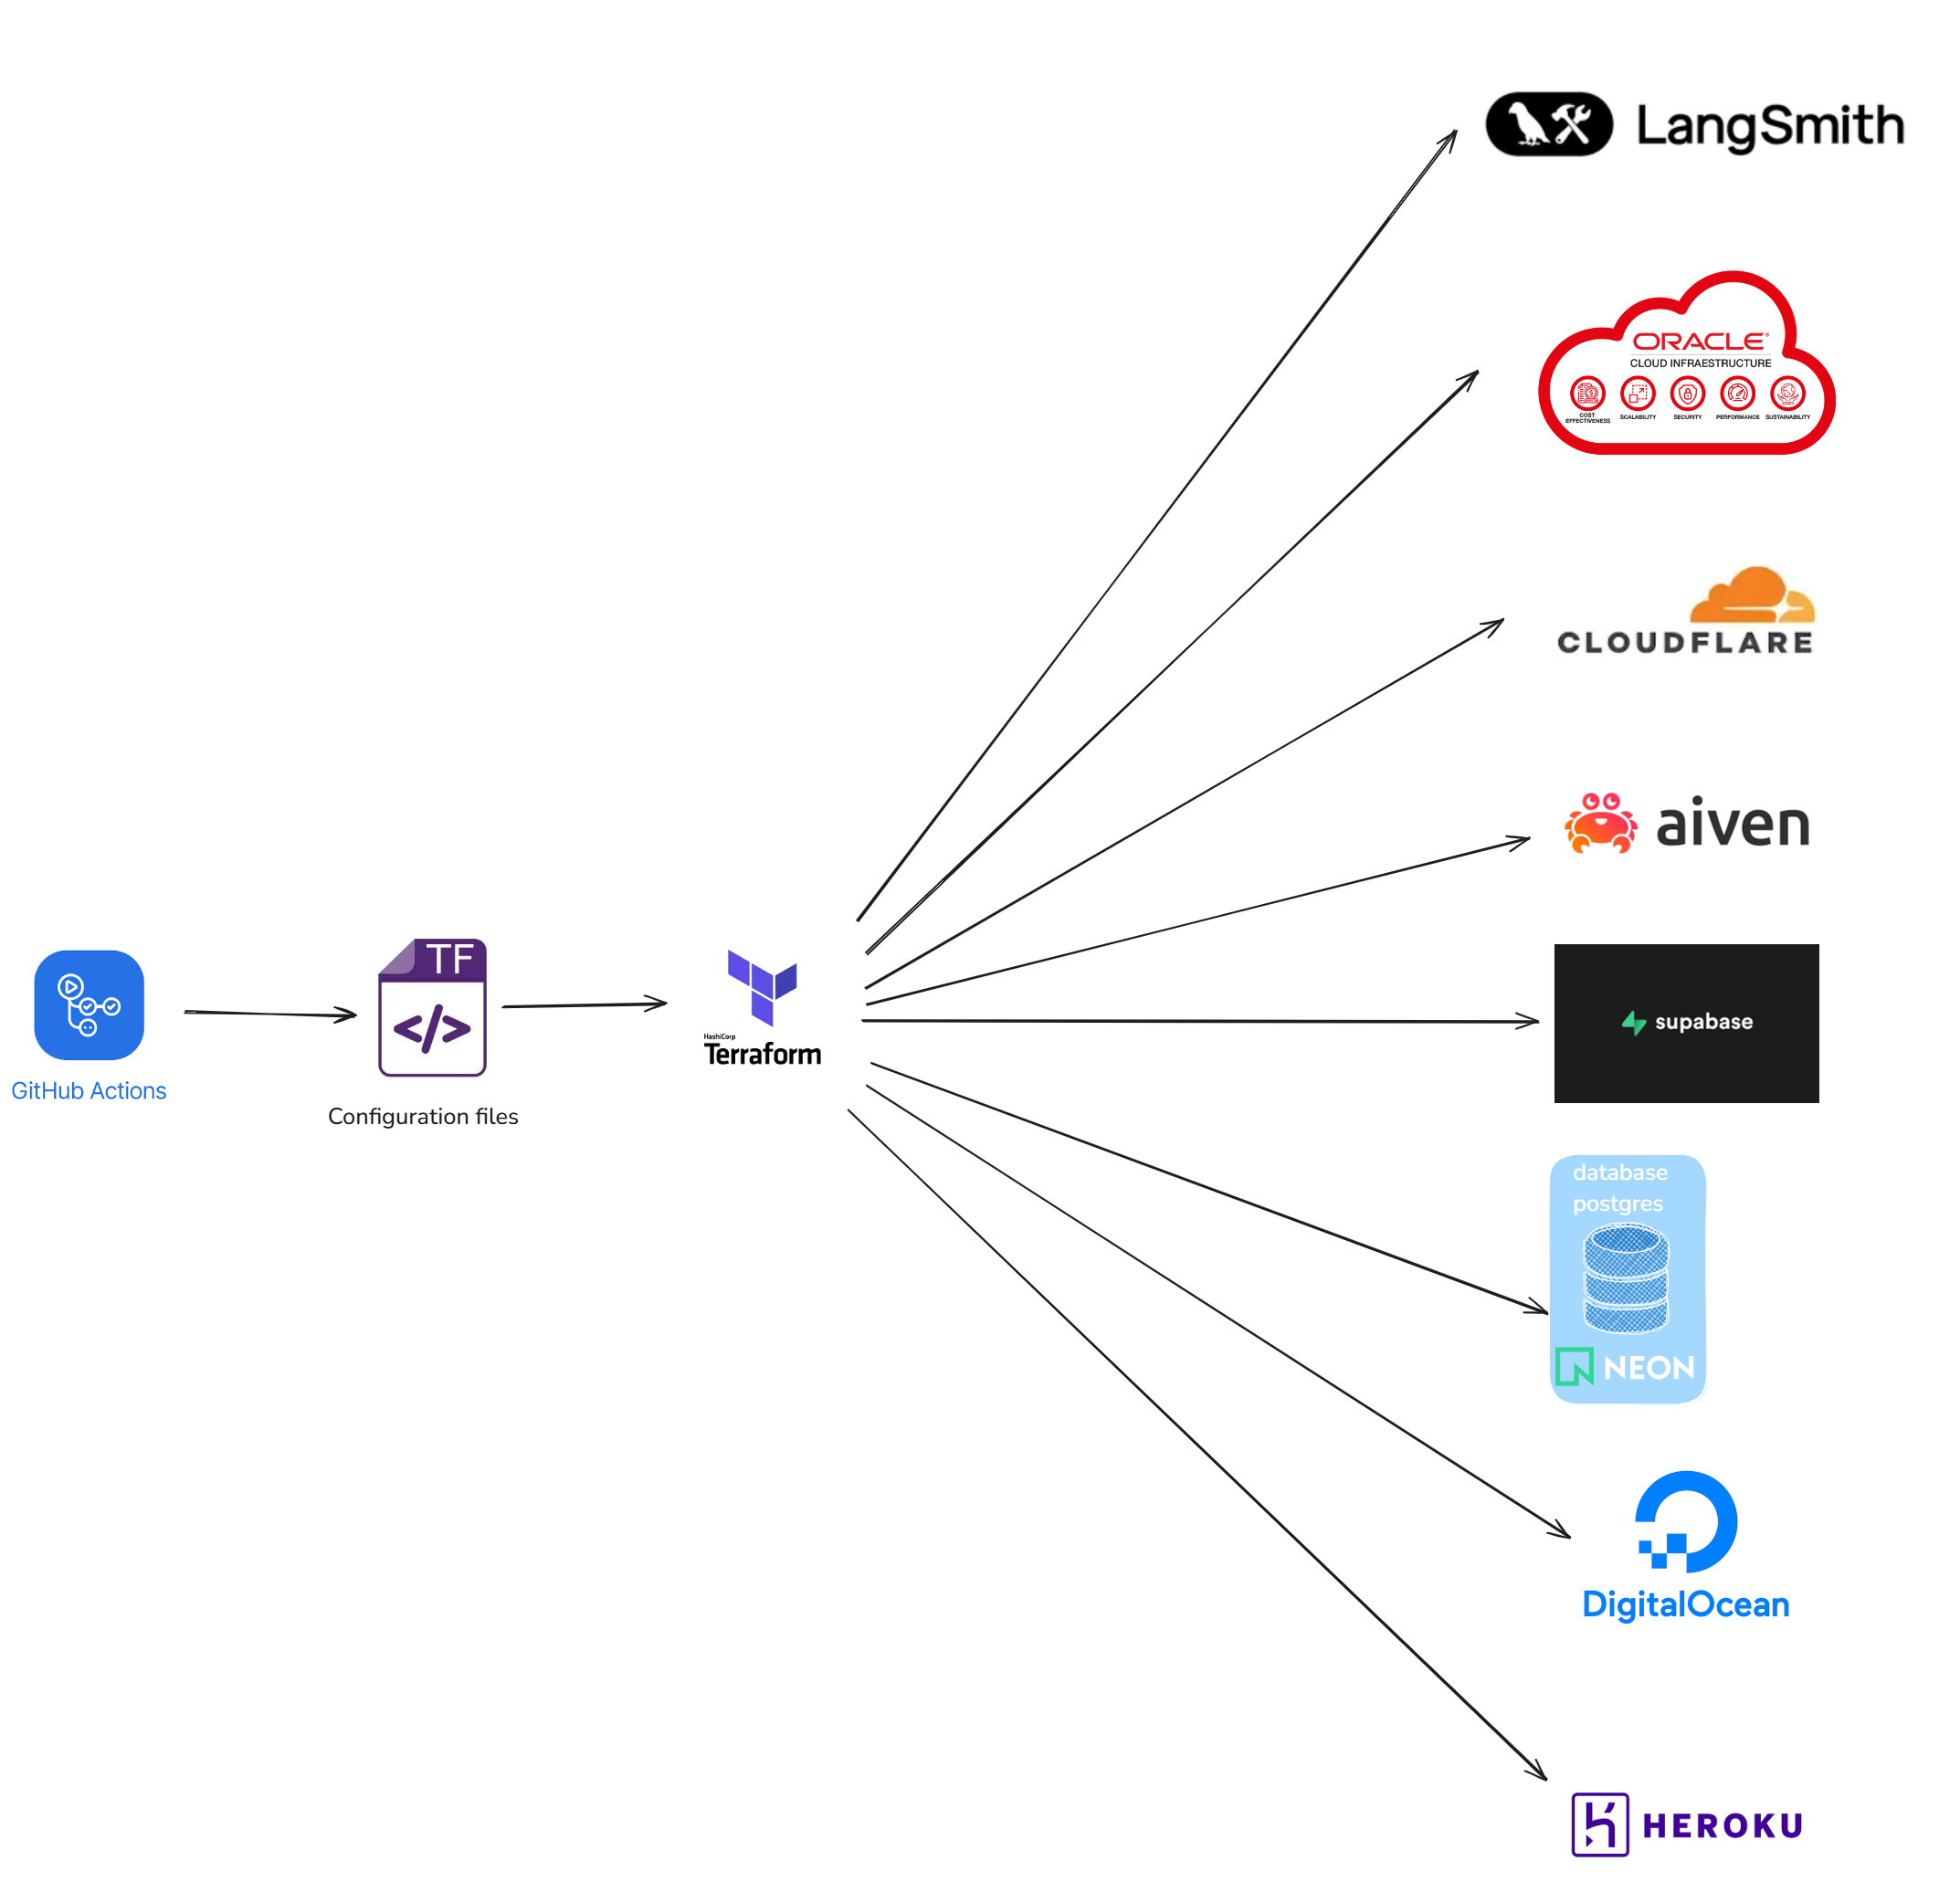
\includegraphics[height=0.7\textheight,width=0.9\textwidth,keepaspectratio]{pictures/infrastructure-as-code-IaC-terraform.excalidraw.png}
\caption{Sơ đồ tổng quan quản lý hạ tầng bằng Terraform trong dự án}
\end{figure}

\note{
Để quản lý hạ tầng một cách nhất quán và tự động, dự án sử dụng Terraform dưới dạng Infrastructure as Code (IaC).
Terraform tự động khởi tạo và cấu hình các tài nguyên bên thứ ba như: Supabase (Auth), LangSmith (giám sát RAG), Cloudflare (DNS và R2 Storage), Neon (PostgreSQL cho các vi dịch vụ), DigitalOcean (Crawl DB) và Heroku (Payment Service). Trạng thái hạ tầng được lưu trữ tập trung trên Terraform Cloud.
}
\end{frame}

\input{contents/Cau_hinh_Kong_API_Gateway_bang_Declarative_Configuration}
\begin{frame}{Kết quả Docker Image trên Docker Hub}
\begin{figure}[H]
\centering
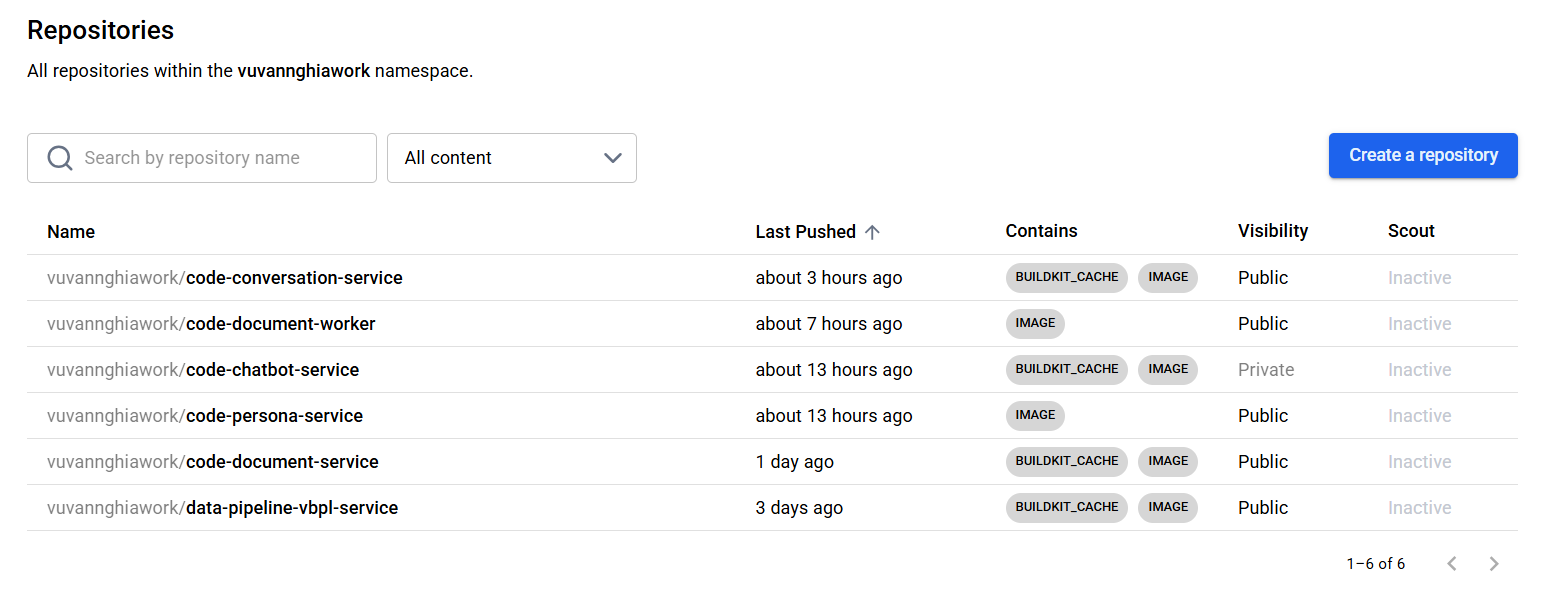
\includegraphics[height=0.55\textheight,width=0.9\textwidth,keepaspectratio]{pictures/docker-hub-web-ui2.png}
\caption{Kết quả Docker Image được push lên Docker Hub}
% \caption{Kết quả giao diện docker}
\end{figure}

\note{
docker
}
\end{frame}

\begin{frame}{Cấu hình tài nguyên Kubernetes trong GitOps Repository}
\begin{figure}[H]
\centering
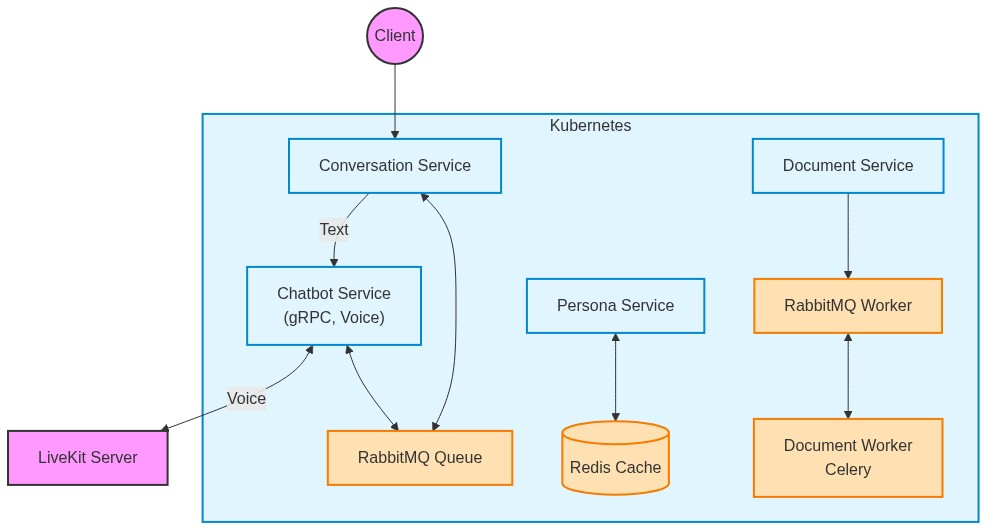
\includegraphics[height=0.55\textheight,width=0.9\textwidth,keepaspectratio]{pictures/Kubernetes.png}
\caption{Cấu hình Kubernetes trong kho lưu trữ GitOps của dự án}
\end{figure}

\note{
Đây là cấu trúc thư mục chứa các file cấu hình Kubernetes (YAML) trong kho lưu trữ GitOps của dự án.
Các dịch vụ nội bộ như RabbitMQ, Redis được chạy trực tiếp trong cụm để giảm độ trễ và được cấu hình dưới dạng ClusterIP để tăng tính bảo mật, ngăn chặn các truy cập trực tiếp từ internet. Các dịch vụ chạy bất đồng bộ như Voice Agent hay Document Worker cũng không công khai service ra bên ngoài.
}
\end{frame}


\begin{frame}{Giao diện quản lý GitOps bằng ArgoCD}
\begin{figure}[H]
\centering
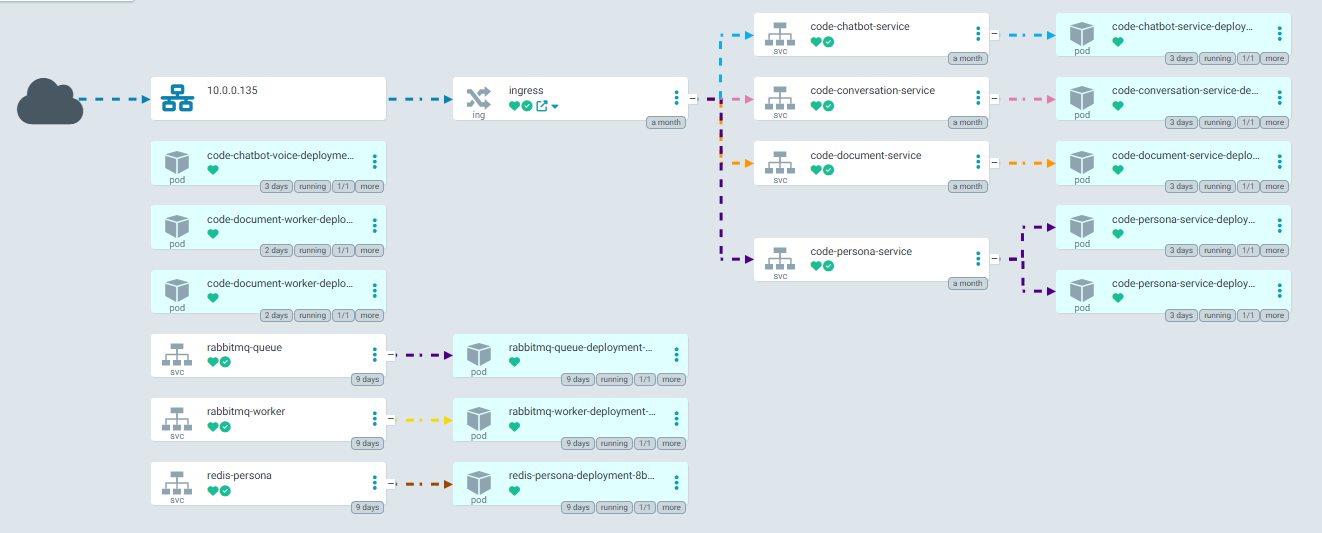
\includegraphics[height=0.55\textheight,width=0.9\textwidth,keepaspectratio]{pictures/argocd-web-ui.png}
\caption{Kết quả giao diện ArgoCD chạy docker trong kubernetes}
\end{figure}

\note{
ArgoCD được triển khai trong cụm Kubernetes để thực hiện quy trình Continuous Delivery (CD) theo mô hình GitOps.
ArgoCD liên tục giám sát kho lưu trữ Git chứa các file cấu hình Kubernetes. Khi phát hiện có sự thay đổi (ví dụ: phiên bản Docker image mới), ArgoCD sẽ tự động đồng bộ (sync) và cập nhật các Pod đang chạy trên Kubernetes thực tế để khớp với cấu hình được khai báo trên Git.
}
\end{frame}


\else
\begin{titlepage}
\thispagestyle{empty}
% \thisfancypage{
% \setlength{\fboxsep}{3pt}
% \fbox}{}
\begin{center}

{\textbf{\large{ĐẠI HỌC BÁCH KHOA HÀ NỘI}}}\\
{\textbf{\large{KHOA TOÁN - TIN}}}\\[5cm]

{\textbf{\huge{ĐỒ ÁN TỐT NGHIỆP}}}\\[1cm]
{\textbf{\Large{Xây dựng ứng dụng hỗ trợ tư vấn pháp luật \\ sử dụng công nghệ trí tuệ nhân tạo}}\\[1cm]

{\textbf{\large{VŨ VĂN NGHĨA}}}\\
{\large{Email: nghia.vv206205@sis.hust.edu.vn}}\\
{\large{Mã sinh viên: 20206205}}\\[0.5cm]

% {\textbf{\large{Chương trình đào tạo: Công nghệ thông tin Việt-Nhật}}}\\
{\textbf{\large{Chuyên ngành Toán - Tin}}}\\

\vspace{4cm}
% Please add the following required packages to your document preamble:
% \usepackage{graphicx}
\begin{table}[H]
\centering
\resizebox{\textwidth}{!}{%
\begin{tabular}{ll}
\multicolumn{1}{c}{\textbf{Giảng viên hướng dẫn:}} & TS. Trần Anh Tú \hspace{0.5cm} \underline{\hspace{3cm}} \\[0.5cm]
& \multicolumn{1}{r}{Chữ kí GVHD} \\[4cm]
% \textbf{Khoa:} & Kỹ thuật máy tính \\[0.5cm]
% \textbf{Trường:} & Công nghệ Thông tin và Truyền thông \\[4cm]
\multicolumn{2}{c}{\textbf{HÀ NỘI, 06/2026}}
\end{tabular}%
}
\end{table}}
\end{center}

\end{titlepage}

\begin{titlepage}
\thispagestyle{empty}
% \thisfancypage{
% \setlength{\fboxsep}{3pt}
% \fbox}{}
\begin{center}

{\textbf{\large{ĐẠI HỌC BÁCH KHOA HÀ NỘI}}}\\
{\textbf{\large{KHOA TOÁN - TIN}}}\\[5cm]

{\textbf{\huge{ĐỒ ÁN TỐT NGHIỆP}}}\\[1cm]
{\textbf{\Large{Xây dựng ứng dụng hỗ trợ tư vấn pháp luật \\ sử dụng công nghệ trí tuệ nhân tạo}}\\[1cm]

{\textbf{\large{VŨ VĂN NGHĨA}}}\\
{\large{Email: nghia.vv206205@sis.hust.edu.vn}}\\
{\large{Mã sinh viên: 20206205}}\\[0.5cm]

% {\textbf{\large{Chương trình đào tạo: Công nghệ thông tin Việt-Nhật}}}\\
{\textbf{\large{Chuyên ngành Toán - Tin}}}\\

\vspace{4cm}
% Please add the following required packages to your document preamble:
% \usepackage{graphicx}
\begin{table}[H]
\centering
\resizebox{\textwidth}{!}{%
\begin{tabular}{ll}
\multicolumn{1}{c}{\textbf{Giảng viên hướng dẫn:}} & TS. Trần Anh Tú \hspace{0.5cm} \underline{\hspace{3cm}} \\[0.5cm]
& \multicolumn{1}{r}{Chữ kí GVHD} \\[4cm]
% \textbf{Khoa:} & Kỹ thuật máy tính \\[0.5cm]
% \textbf{Trường:} & Công nghệ Thông tin và Truyền thông \\[4cm]
\multicolumn{2}{c}{\textbf{HÀ NỘI, 06/2026}}
\end{tabular}%
}
\end{table}}
\end{center}

\end{titlepage}

\newpage

\vspace*{\fill}
\begin{center}
% Trang này chỉ để trống!
\thispagestyle{empty}
\end{center}
\vspace*{\fill}

\newpage

% \restoregeometry

% \newpage

\newpage
\thispagestyle{empty}

% 1. BẮT ĐẦU CÔ LẬP: Mọi thiết lập font chữ trong này sẽ không ảnh hưởng trang khác
\begingroup

% Nếu bạn cần đổi lề riêng cho trang này, hãy bỏ comment dòng dưới:
% \newgeometry{left=2.2cm,right=2.8cm,top=2cm,bottom=2cm}
% \pagenumbering{roman}
% \setcounter{page}{1}
% \thisfancypage{
% 	\setlength{\fboxsep}{0.5cm}
% 	\fbox}{}

\begin{tikzpicture}[remember picture, overlay]
\path ($(current page text area.north east)+(0.5cm, 0.5cm)$) coordinate (A)
($(current page text area.north west)+(-0.5cm, 0.5cm)$) coordinate (B)
($(current page text area.south west)+(-0.5cm, -0.5cm)$) coordinate (C)
($(current page text area.south east)+(0.5cm, -0.5cm)$) coordinate (D);
\draw[black!40!black, line width=3pt]
(A)--(B)--(C)--(D)--cycle;
\draw[black!10!black, line width=0.5pt]
($(A)+(-0.1cm, -0.1cm)$)--($(B)+(0.1cm, -0.1cm)$)--($(C)+(0.1cm, 0.1cm)$)--($(D)+(-0.1cm, 0.1cm)$)--cycle;
\end{tikzpicture}

\fontsize{13pt}{16pt}\selectfont
\bigbreak
\begin{center}
{\bfseries NHẬN XÉT CỦA GIẢNG VIÊN HƯỚNG DẪN}

\end{center}
\bigbreak

\fontsize{12pt}{14pt}\selectfont

\begin{enumerate}

\item [{\bfseries 1.}]{\bfseries Mục đích và nội dung của đồ án}

\begin{enumerate}
\item Phân tích thiết kế hệ thống chatbot tư vấn pháp luật với dữ liệu thực tế
\item Tìm hiểu và lựa chọn công nghệ xây dựng chatbot phù hợp với bài toán đặt ra
\item Triển khai xây dựng và lập trình hệ thống
\end{enumerate}

\item [{\bfseries 2.}] {\bfseries Kết quả đạt được}

\begin{enumerate}
\item Tìm hiểu và tích hợp nhiều công nghệ có tính cập nhật và độ khó cao trong Đồ án
\item Triển khai data pipeline, thu thập, xử lý và lưu trữ dữ liệu văn bản pháp luật
\item Triển khai xây dựng và lập trình hệ thống có chức năng đúng yêu cầu đặt ra
\end{enumerate}

\item [{\bfseries 3.}]{\bfseries Ý thức làm việc của sinh viên}

\begin{enumerate}
\item Sinh viên chủ động, tích cực trong việc tìm hiểu các công nghệ mới để đưa vào đồ án theo định hướng
\item Sinh viên thực hiện nội dung đúng tiến độ và chủ động báo cáo, xin góp ý hoàn thiện.
\item Sinh viên có ý thức luôn cải tiến, hoàn thiện sản phẩm
\end{enumerate}
\end{enumerate}
\hspace{0.4\textwidth}
\begin{minipage}{0.5\textwidth}
\noindent\begin{center}
\textit{Hà Nội, ngày \dots tháng \dots năm \dots} \\

Giảng viên hướng dẫn \\
\textit{(Ký và ghi rõ họ tên)} \\
\vspace{2cm}
% \textbf{TS. Trần Anh Tú}

\end{center}
\end{minipage}

% 2. KẾT THÚC CÔ LẬP: Trả lại font chữ ban đầu
\endgroup

\newpage
% 3. TRẢ LẠI LỀ GỐC: Nếu ở trên bạn dùng \newgeometry, thì bắt buộc phải bỏ comment dòng dưới
% \restoregeometry
% \restoregeometry

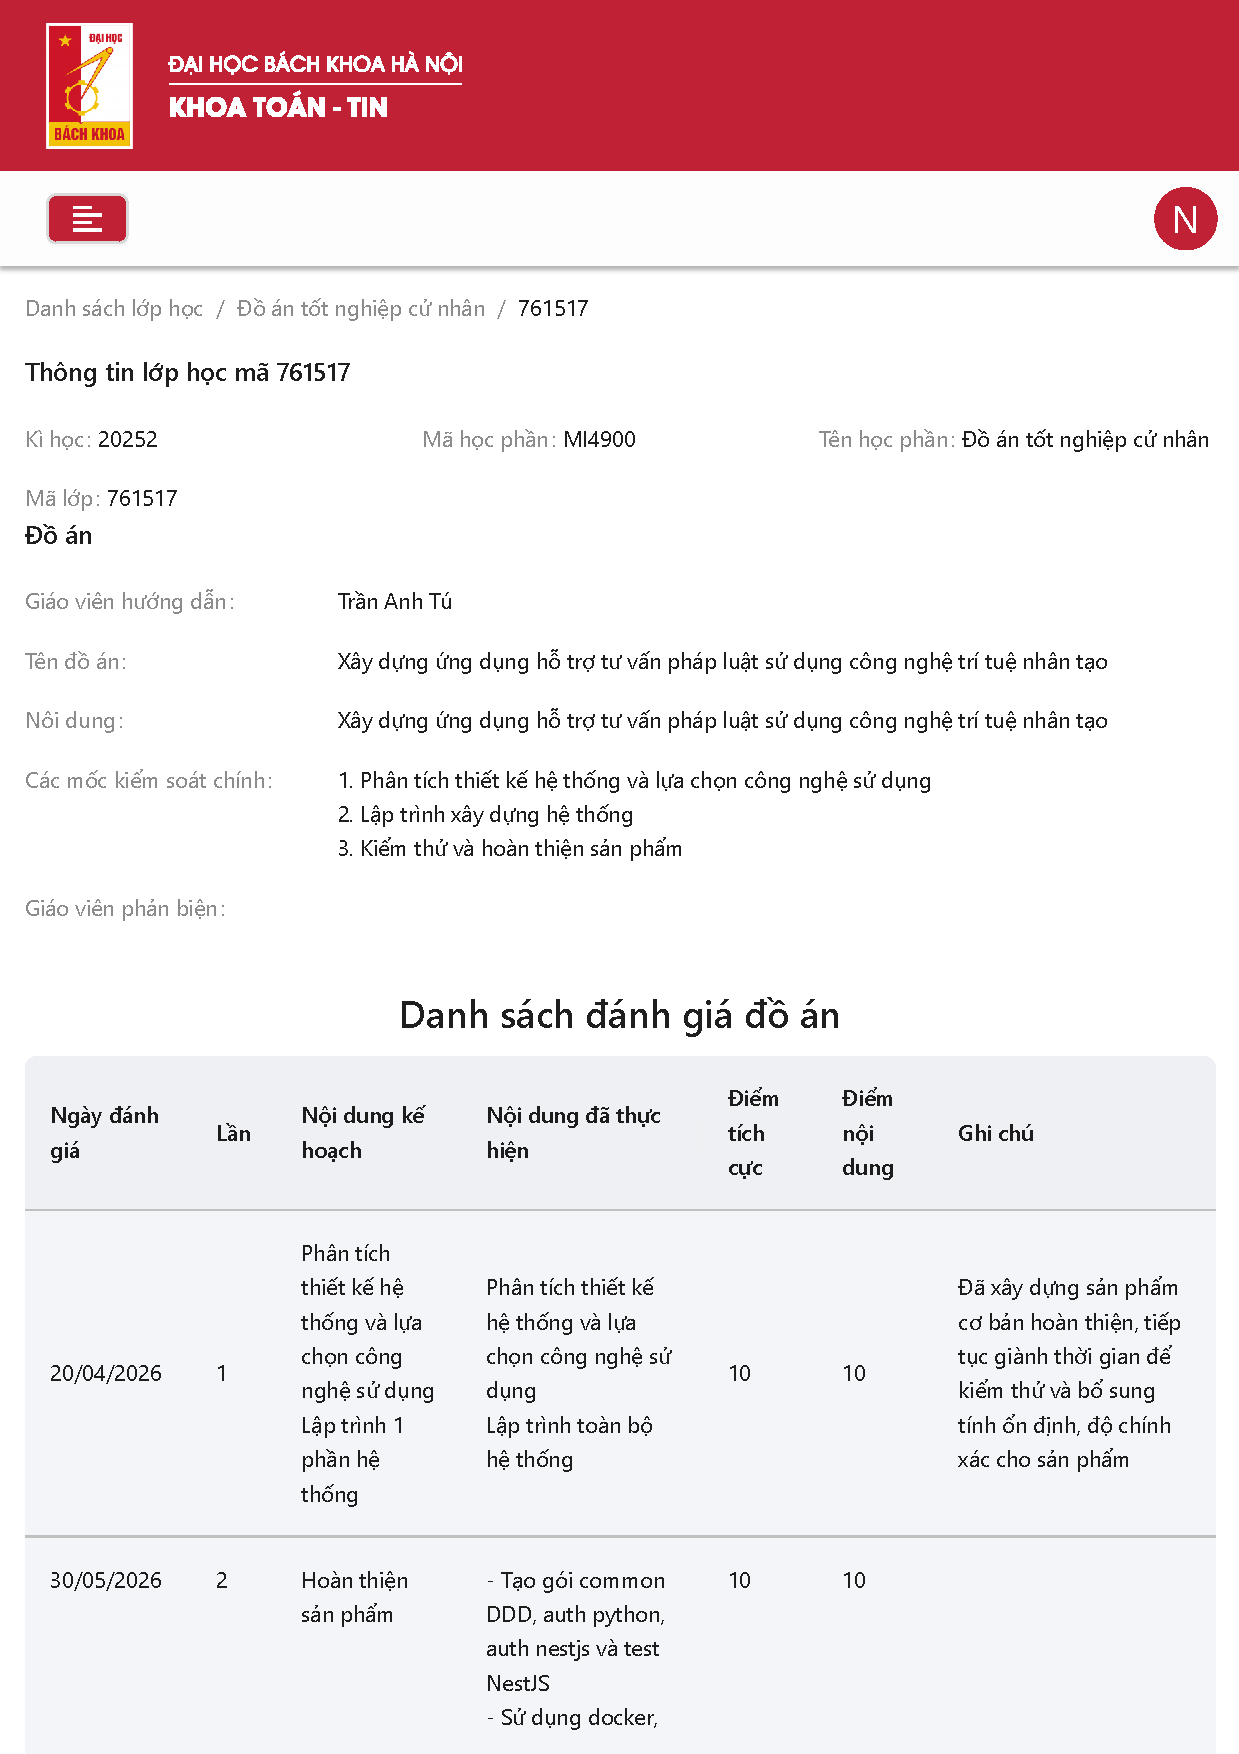
\includepdf[pages=-]{contents/0/bao_cao/danh_gia2.pdf}
{\centering \section*{Lời cảm ơn}}

Qua thời gian học tập và rèn luyện tại
\textit{Đại học Bách khoa Hà Nội},
đến nay em đã hoàn thành đồ án tốt nghiệp.
Trong thời gian học tập để có được kết quả hiện tại
em xin chân thành cảm ơn tới các thầy cô giảng viên trong \textit{Khoa Toán Tin}
đã giảng dạy, quan tâm và tạo điều kiện thuận lợi để em học tập rèn luyện trong suốt thời gian qua,
giúp em trang bị những kiến thức, kỹ năng cần thiết
để em có thể hoàn thành tốt nhất báo cáo này
với
đề tài:
\textit{Xây dựng ứng dụng hỗ trợ tư vấn pháp luật sử dụng công nghệ trí tuệ nhân tạo}.

Đồng thời, em xin gửi lời cảm ơn chân thành và sâu sắc đến \textit{Thầy TS. Trần Anh Tú},
người thầy đã tận tình hỗ trợ,
giúp đỡ và hướng dẫn em suốt thời gian thực hiện đồ án.
Những kiến thức và kinh nghiệm mà em đã tiếp thu được trong quá trình này
sẽ đóng góp quan trọng vào sự phát triển và thành công của em trong tương lai.
Em xin gửi lời chúc sức khỏe tốt nhất đến thầy,
hy vọng thầy luôn dồi dào sức khỏe, đam mê và nhiệt huyết trong công việc giảng dạy.

Em cũng xin gửi lời cảm ơn tới bố mẹ
đã dành nhiều thời gian chăm lo, động viên
và giúp đỡ em để em đạt được thành công trong học tập.

Mặc dù đã cố gắng nỗ lực học hỏi để hoàn thành đồ án,
nhưng thời gian thực hiện đồ án có hạn,
kiến thức của em còn hạn chế.
Do vậy,
không tránh khỏi những thiếu sót,
em rất mong nhận được những ý kiến đóng góp quý báu của thầy cô
để em có thể cải thiện một cách tốt nhất.

\vspace{0.5cm} \emph{Em xin chân thành cảm ơn!}

%%%%%%%%%%%%%%%%%%%%%%%%%%%%%%%%%%%%%%%%%%%%%%%%%%%%%%%
%%%%%%%%%%%%%%%%%%%%%%%%%%%%%%%%%%%%%%%%%%%%%%%%%%%%%%%
%%%%%%%%%%%%%%%%%%%%%%%%%%%%%%%%%%%%%%%%%%%%%%%%%%%%%%%

{\centering \section*{Tóm tắt nội dung đồ án}}

% {
% \color{RedHUST}

% Tóm tắt nội dung của đồ án tốt nghiệp trong khoảng tối đa 300 chữ.
% Phần tóm tắt cần nêu được các ý:
% vấn đề cần thực hiện;
% phương pháp thực hiện;
% công cụ sử dụng (phần mềm, phần cứng…);
% kết quả của đồ án có phù hợp với các vấn đề đã đặt ra hay không;
% tính thực tế của đồ án,
% định hướng phát triển mở rộng của đồ án (nếu có);
% các kiến thức và kỹ năng mà sinh viên đã đạt được.

% }

Đồ án
được thực hiện nhằm giải quyết nhu cầu tra cứu
và giải đáp thông tin pháp luật Việt Nam
(bao gồm Văn bản pháp luật và Pháp Điển) một cách chính xác, nhanh chóng và tự động hóa.

Để tối ưu năng lực giải đáp,
đồ án triển khai hệ thống
Agentic RAG nâng cao sử dụng LangGraph.

Về mặt kiến trúc, hệ thống được thiết kế theo kiến trúc vi dịch vụ (Microservice Architecture),
ứng dụng phương pháp Thiết kế hướng miền (Domain-Driven Design - DDD)
và các dịch vụ được điều phối qua Kong API Gateway.

Để đảm bảo tính ổn định,
hiệu năng cao,
tận dụng điểm mạnh tài nguyên,
thế mạnh framework ngôn ngữ lập trình
và khả năng mở rộng,
các dịch vụ giao tiếp đa dạng từ gRPC cho trò chuyện trực tiếp,
giao tiếp bất đồng bộ giữa các dịch vụ NestJS và Python
được xử lý thông qua RabbitMQ.
Luồng nghiệp vụ
quy trình thanh toán thuê bao VIP
qua các cổng nội địa (VNPay, MoMo, ZaloPay, SePay),
được đồng bộ
sự kiện
bằng nền tảng Kafka.
Toàn bộ vòng đời ứng dụng
được tự động hóa thông qua
CI/CD trên GitHub Actions,
đóng gói bằng Docker và triển khai vận hành trên
cụm Kubernetes thông qua ArgoCD.

Đồ án đã vận hành thành công một trợ lý pháp luật,
đưa ra các tư vấn pháp lý với các bước suy luận logic
và trích dẫn nguồn văn bản rõ ràng.
Bên cạnh đó,
ứng dụng còn mang đến trải nghiệm đàm thoại
thời gian thực bằng cách tích hợp LiveKit
cùng các mô hình xử lý giọng nói tiên tiến như Whisper (Speech-to-Text), Edge, Piper và ElevenLabs (Text-to-Speech).

\begin{flushright}
\begin{tabular}{c}
% Hà Nội, \today \\
\textit{Hà Nội, ngày \dots tháng \dots năm \dots} \\
Sinh viên thực hiện \\
\textit{(Ký và ghi rõ họ tên)} \\
% Nghĩa \\
% Vũ Văn Nghĩa
\end{tabular}
\end{flushright}

\newpage

\renewcommand{\contentsname}{MỤC LỤC} % ĐẶT TÊN TIÊU ĐỀ MỤC LỤC
\tableofcontents

\newpage

% DANH MỤC KÝ HIỆU

\newpage
\phantomsection
{\centering \section*{DANH MỤC KÝ HIỆU}} % Đặt tên tiêu đề
\addcontentsline{toc}{section}{DANH MỤC KÝ HIỆU} % Thêm vào mục lục

\begin{table}[ht]
\centering
\small
\begin{tabular}{|c|p{2.1cm}|p{4.3cm}|p{5.4cm}|}
\hline
\textbf{STT} & \textbf{Từ viết tắt} & \textbf{Từ viết đầy đủ} & \textbf{Mô tả} \\ \hline
1 & 2FA & Two-Factor Authentication & Xác thực hai yếu tố \\ \hline
2 & AAL1 / AAL2 & \makecell[l]{Authenticator Assurance \\ Level 1 / 2} & Mức độ đảm bảo xác thực 1 / 2 \\ \hline
3 & AI & Artificial Intelligence & Trí tuệ nhân tạo \\ \hline
4 & API & \makecell[l]{Application Programming \\ Interface} & Giao diện lập trình ứng dụng \\ \hline
5 & CD & \makecell[l]{Continuous \\ Delivery / Deployment} & Chuyển giao/Triển khai liên tục \\ \hline
6 & CI & Continuous Integration & Tích hợp liên tục \\ \hline
7 & CLI & Command Line Interface & Giao diện dòng lệnh \\ \hline
8 & CSDL & Cơ sở dữ liệu & Cơ sở dữ liệu \\ \hline
9 & DB & Database & Cơ sở dữ liệu \\ \hline
10 & DDD & Domain Driven Design & Thiết kế hướng miền \\ \hline
11 & DLQ & Dead Letter Queue & Hàng đợi thư lỗi \\ \hline
12 & DNS & Domain Name System & Hệ thống phân giải tên miền \\ \hline
13 & HTML & Hyper Text Markup Language & Ngôn ngữ Đánh dấu Siêu văn bản \\ \hline
14 & IPN & Instant Payment Notification & Thông báo thanh toán tức thì \\ \hline
15 & IaC & Infrastructure as Code & Cơ sở hạ tầng dưới dạng mã \\ \hline
16 & JWT & JSON Web Token & Tiêu chuẩn truyền tải thông tin JSON \\ \hline
17 & K8s & Kubernetes & Công cụ quản lý container \\ \hline
18 & LLM & Large Language Model & Mô hình ngôn ngữ lớn \\ \hline
19 & LRU & Least Recently Used & \makecell[l]{Thuật toán loại bỏ dữ liệu \\ ít được sử dụng gần đây nhất} \\ \hline
20 & MFA & Multi-Factor Authentication & Xác thực đa yếu tố \\ \hline
21 & NLP & Natural Language Processing & Xử lý ngôn ngữ tự nhiên \\ \hline
22 & PSC & Payment Service Consumer & Đơn vị sử dụng dịch vụ thanh toán \\ \hline
23 & PSP & Payment Service Provider & Đơn vị cung cấp dịch vụ thanh toán \\ \hline
24 & QR Code & Quick Response Code & Mã phản hồi nhanh \\ \hline
25 & RAG & \makecell[l]{Retrieval Augmented \\ Generation} & Tạo tăng cường truy xuất \\ \hline
26 & RLS & Row-Level Security & Bảo mật cấp hàng \\ \hline
27 & SMTP & Simple Mail Transfer Protocol & Giao thức truyền thư đơn giản \\ \hline
28 & SQL & Structured Query Language & Ngôn ngữ truy vấn cấu trúc \\ \hline
29 & SSE & Server-sent events & Sự kiện máy chủ gửi \\ \hline
30 & STT & Speech to Text & Chuyển giọng nói thành văn bản \\ \hline
31 & TOTP & \makecell[l]{Time-based \\ One-Time Password} & \makecell[l]{Mật khẩu dùng một lần \\ dựa trên thời gian} \\ \hline
32 & TTL & Time To Live & Thời gian tồn tại \\ \hline
33 & TTS & Text to Speech & Chuyển văn bản thành giọng nói \\ \hline
34 & UI & User Interface & Giao diện người dùng \\ \hline
35 & UML & Unified Modeling Language & Ngôn ngữ mô hình hóa thống nhất \\ \hline
36 & URL & Uniform Resource Locator & Trình định vị tài nguyên đồng nhất \\ \hline
37 & UUID & Universally Unique Identifier & Mã định danh duy nhất toàn cầu \\ \hline
38 & VBPL & Văn bản pháp luật & Văn bản pháp luật \\ \hline
39 & VIP & Very Important Person & Người rất quan trọng \\ \hline
40 & VPS & Virtual Private Server & Máy chủ riêng ảo \\ \hline
41 & gRPC & gRPC Remote Procedure Call & \makecell[l]{Framework Gọi thủ tục từ xa \\ do Google phát triển} \\ \hline
\end{tabular}
\end{table}

\newpage

% DANH MỤC HÌNH VẼ

\newpage
\phantomsection

\renewcommand{\listfigurename}{DANH MỤC HÌNH VẼ} % ĐẶT TÊN TIÊU ĐỀ
\addcontentsline{toc}{section}{DANH MỤC HÌNH VẼ} % THÊM VÀO MỤC LỤC
\makeatletter
\renewcommand*\l@figure{\@dottedtocline{1}{1.5em}{5.5em}}
\makeatother
{\let\oldnumberline\numberline
\renewcommand{\numberline}[1]{\oldnumberline{Hình~#1}}
\listoffigures}

\newpage

% DANH MỤC BẢNG BIỂU

\newpage
\phantomsection

\renewcommand{\listtablename}{DANH MỤC BẢNG BIỂU}
\makeatletter
\renewcommand{\listoftables}{
\begin{center}
\section*{\listtablename}
\end{center}
\@starttoc{lot}
}
\renewcommand*\l@table{\@dottedtocline{1}{1.5em}{5.5em}}
\makeatother
\addcontentsline{toc}{section}{DANH MỤC BẢNG BIỂU}
{\let\oldnumberline\numberline
\renewcommand{\numberline}[1]{\oldnumberline{Bảng~#1}}
\listoftables}

\newpage

%%%%%%%%%%%%%%%%%%%%%%%%%%%%%%%%%%%%%%%%%%%%%%%%%%%%%%%
% % % % \section{Bài toán nghiệp vụ}

% % % % \begin{frame}{Sự cần thiết}

\begin{itemize}

\item Hệ thống pháp luật rất phức tạp

\item Cá nhân, doanh nghiệp bỏ lỡ cập nhật

\end{itemize}

\begin{figure}[H]
\centering

\includegraphics[width=\linewidth,height=0.55\textheight,keepaspectratio]{pictures/chatbot-tra-cuu-luat-la-gi.jpeg}
\caption[AI hỗ trợ tư vấn pháp luật]{AI hỗ trợ tư vấn pháp luật (Nguồn: \footnotemark)}
\end{figure}
\footnotetext{\url{https://vnptai.io/vi/blog/detail/chatbot-ai-tra-cuu-luat}}

\note{

Hệ thống pháp luật rất phức tạp.

\hrule

Các VBPL có thể thay thế, bổ sung VBPL khác,

hoặc bị hết hiệu lực.

\hrule

Nếu cá nhân, doanh nghiệp bỏ lỡ cập nhật

Và vô tình áp dụng sai luật

\hrule

=> Dẫn đến hậu quả tài chính và rủi ro pháp lý

}

\end{frame}

% hệ thống pháp luật rất phức tạp.

% các văn bản pháp luật có thể thay thế, bổ sung văn bản pháp luật khác

% hoặc bị hết hiệu lực. nếu cá nhân, doanh nghiệp bỏ lỡ cập nhật

% và vô tình áp dụng sai luật. dẫn đến hậu quả tài chính và rủi ro pháp lý


% % % % \begin{frame}{Vai trò và chức năng}
\begin{table}
\centering
\caption{Bảng vai trò và chức năng trong hệ thống} % <-- Lệnh caption được thêm ở đây

% Bây giờ cả hai cột đều có thể dùng 'l' (căn trái) hoặc 'c' (căn giữa)
\begin{tabular}{|l|l|}
\hline
\textbf{Vai trò} & \textbf{Chức năng} \\
\hline

% Dòng 1: Guest
Guest &
\makecell[l]{ % [l] để căn trái các dòng bên trong ô
Giới thiệu, nghe thử giọng nói, xem gói VIP \\
Đăng ký email,
Đăng nhập \textbf{
\textcolor{blue}{G}%
\textcolor{red}{o}%
\textcolor{yellow}{o}%
\textcolor{blue}{g}%
\textcolor{green}{l}%
\textcolor{red}{e}
}
} \\
\hline

% Dòng 2: User
User &
\makecell[l]{
Đăng nhập và quản lý tài khoản, cài đặt \\
Thực hiện trò chuyện, đánh dấu và chia sẻ \\
Mua gói VIP và xem lịch sử
} \\
\hline

% Dòng 3: VIP
VIP &
\makecell[l]{
Suy luận nâng cao\\
Tài liệu cá nhân \\
Sử dụng giọng nói
} \\
\hline

% Dòng 4: Admin
Admin &
\makecell[l]{
Quản lý nhân vật,
gói VIP \\
Báo cáo đường ống dữ liệu
} \\
\hline
\end{tabular}
\end{table}
\end{frame}


% % % % \begin{frame}{Sơ đồ Use Case - Khách vãng lai}
\begin{figure}[H]
\centering
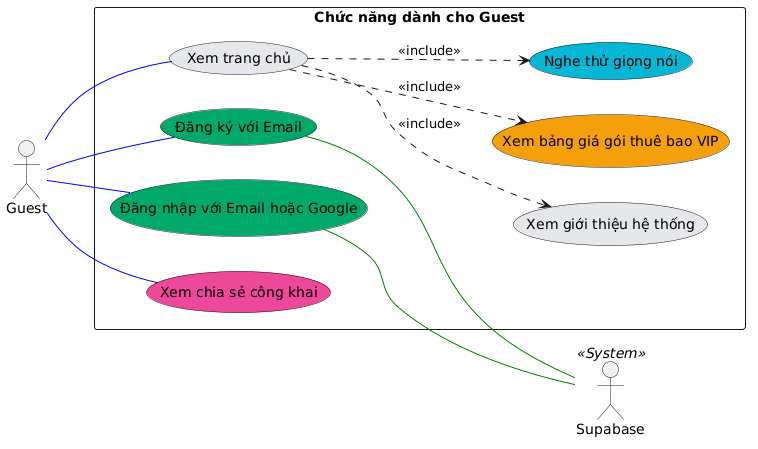
\includegraphics[width=\linewidth,height=0.74\textheight,keepaspectratio]{pictures/UML-UseCase-Guest.png}
\caption{Sơ đồ Use Case chức năng của khách vãng lai}
\end{figure}

\note{

dưới đây là sơ đồ iu cây dành cho người dùng trong hệ thống
\hrule

đầu tiên là khách vãng lai (chưa đăng nhập hệ thống)
\hrule

tiếp theo sơ đồ iu cây dành cho người dùng cơ bản (đã đăng nhập)
\hrule

tiếp theo sơ đồ iu cây dành cho người dùng vip
\hrule

cuối cùng là sơ đồ iu cây dành cho quản trị viên (admin)

}
\end{frame}

% % % % \begin{frame}{Sơ đồ Use Case - Người dùng cơ bản}
\begin{figure}[H]
\centering
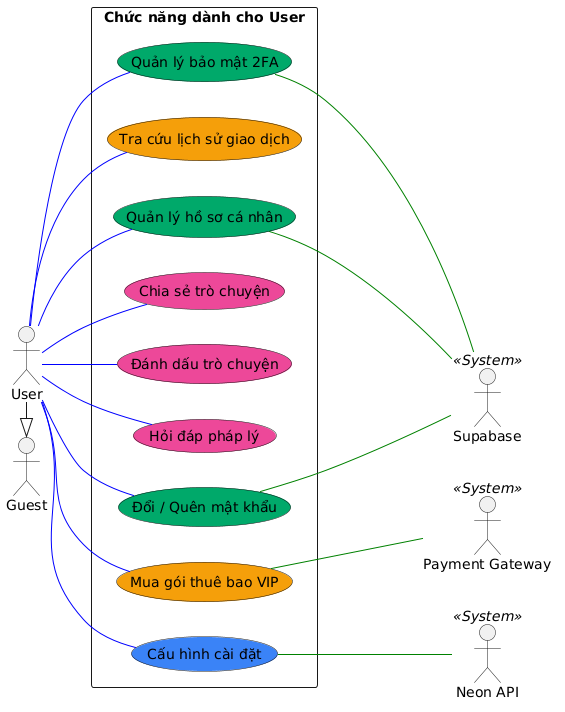
\includegraphics[width=\linewidth,height=0.74\textheight,keepaspectratio]{pictures/UML-UseCase-User.png}
\caption{Sơ đồ Use Case chức năng của người dùng cơ bản}
\end{figure}

\note{

Dưới đây là

Sơ đồ Use Case
chi tiết

dành cho người dùng cơ bản
(đã đăng nhập).

}
\end{frame}

% % % % \begin{frame}{Sơ đồ Use Case - Người dùng VIP}
\begin{figure}[H]
\centering
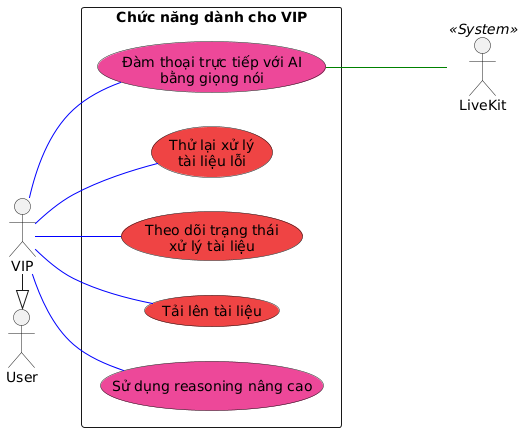
\includegraphics[width=\linewidth,height=0.74\textheight,keepaspectratio]{pictures/UML-UseCase-VIP.png}
\caption{Sơ đồ Use Case chức năng của người dùng VIP}
\end{figure}

\note{

Dưới đây là

Sơ đồ Use Case
chi tiết

dành cho nhóm người dùng VIP.

}
\end{frame}

% % % % \begin{frame}{Sơ đồ Use Case - Quản trị viên}
\begin{figure}[H]
\centering
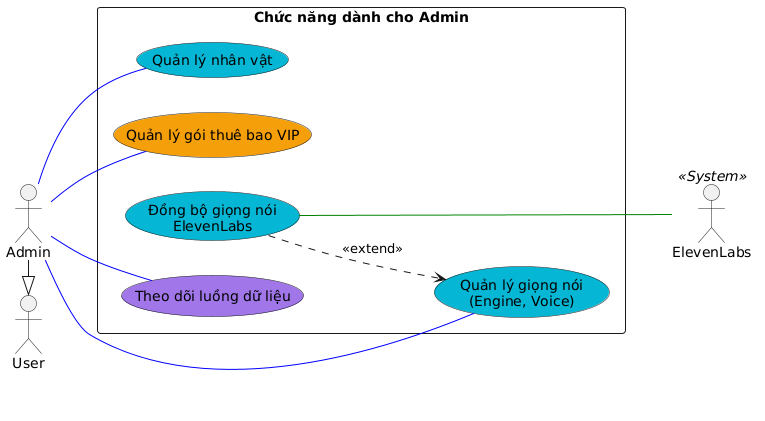
\includegraphics[width=\linewidth,height=0.72\textheight,keepaspectratio]{pictures/UML-UseCase-Admin.png}
\caption{Sơ đồ Use Case chức năng của quản trị viên}
\end{figure}

\note{
Sơ đồ Use Case dành cho quản trị viên (Admin).
Quản trị viên có các quyền hạn cao nhất trong hệ thống bao gồm: quản lý danh sách người dùng, quản lý cấu hình các gói thanh toán VIP, giám sát hệ thống, xem các báo cáo thống kê giao dịch và quản lý các tài liệu pháp luật chung trong CSDL tri thức của hệ thống.
}
\end{frame}


% % % \section{Xây dựng hệ thống AI}
% % % \subsection{Đường ống dữ liệu}

% % % \begin{frame}{Đường ống dữ liệu văn bản pháp luật (VBPL)}
\begin{figure}[H]
\centering
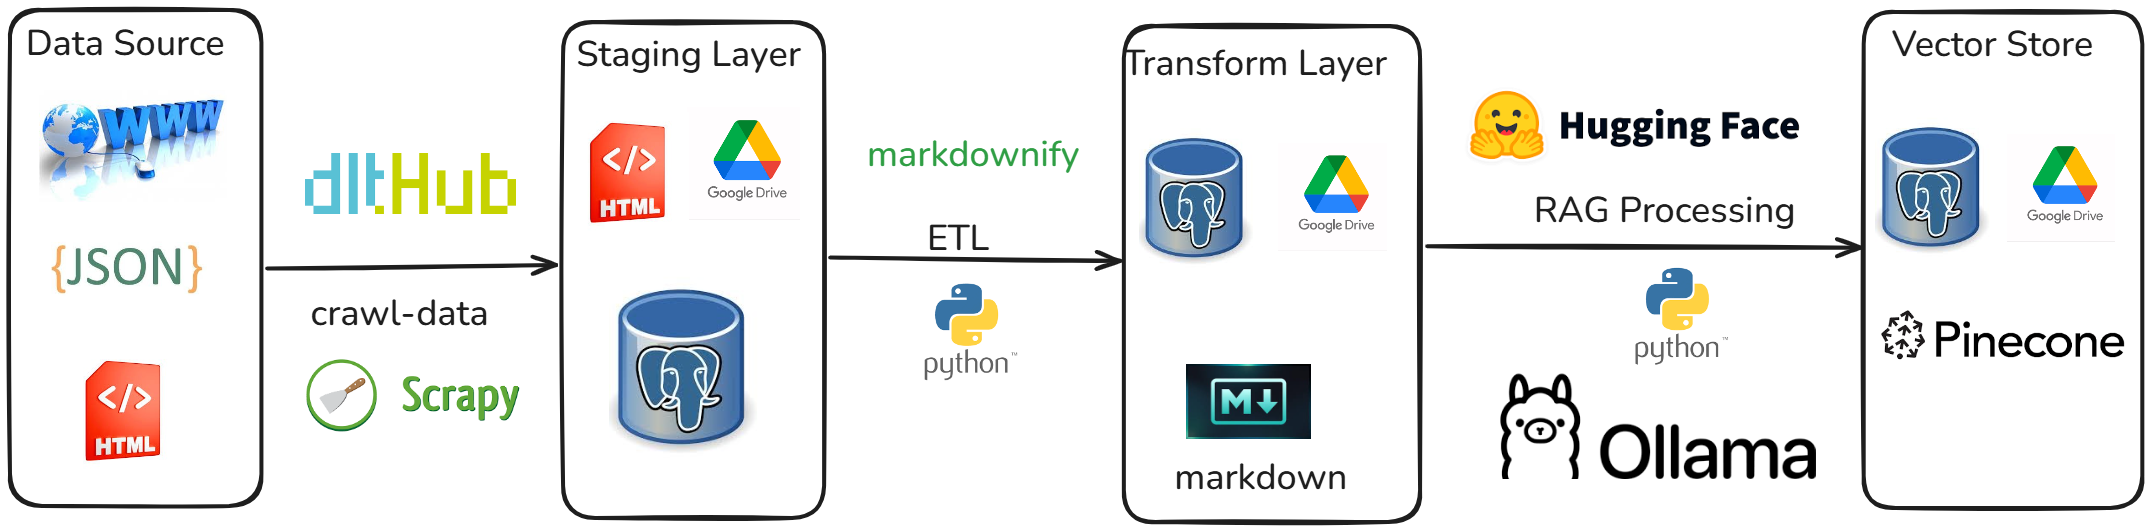
\includegraphics[height=0.55\textheight,width=0.9\textwidth,keepaspectratio]{pictures/Data-Pipeline-VBPL.excalidraw.png}
\caption{Sơ đồ tổng quan luồng dữ liệu văn bản pháp luật mới}
\end{figure}

\note{
Do nguồn dữ liệu Văn bản pháp luật Việt Nam (VBPL) thay đổi cấu trúc trang web và API vào tháng 5/2026, dự án đã xây dựng lại đường ống dữ liệu mới.
Đường ống dữ liệu này tự động hóa quy trình từ thu thập thông tin qua crawler, lưu trữ dữ liệu thô vào PostgreSQL, thực hiện tiền xử lý văn bản pháp luật và cuối cùng là tích hợp vào RAG pipeline để cập nhật CSDL tri thức của trợ lý ảo.
}
\end{frame}

% % % \begin{frame}{Quy trình các bước thu thập dữ liệu văn bản pháp luật}
\begin{figure}[H]
\centering
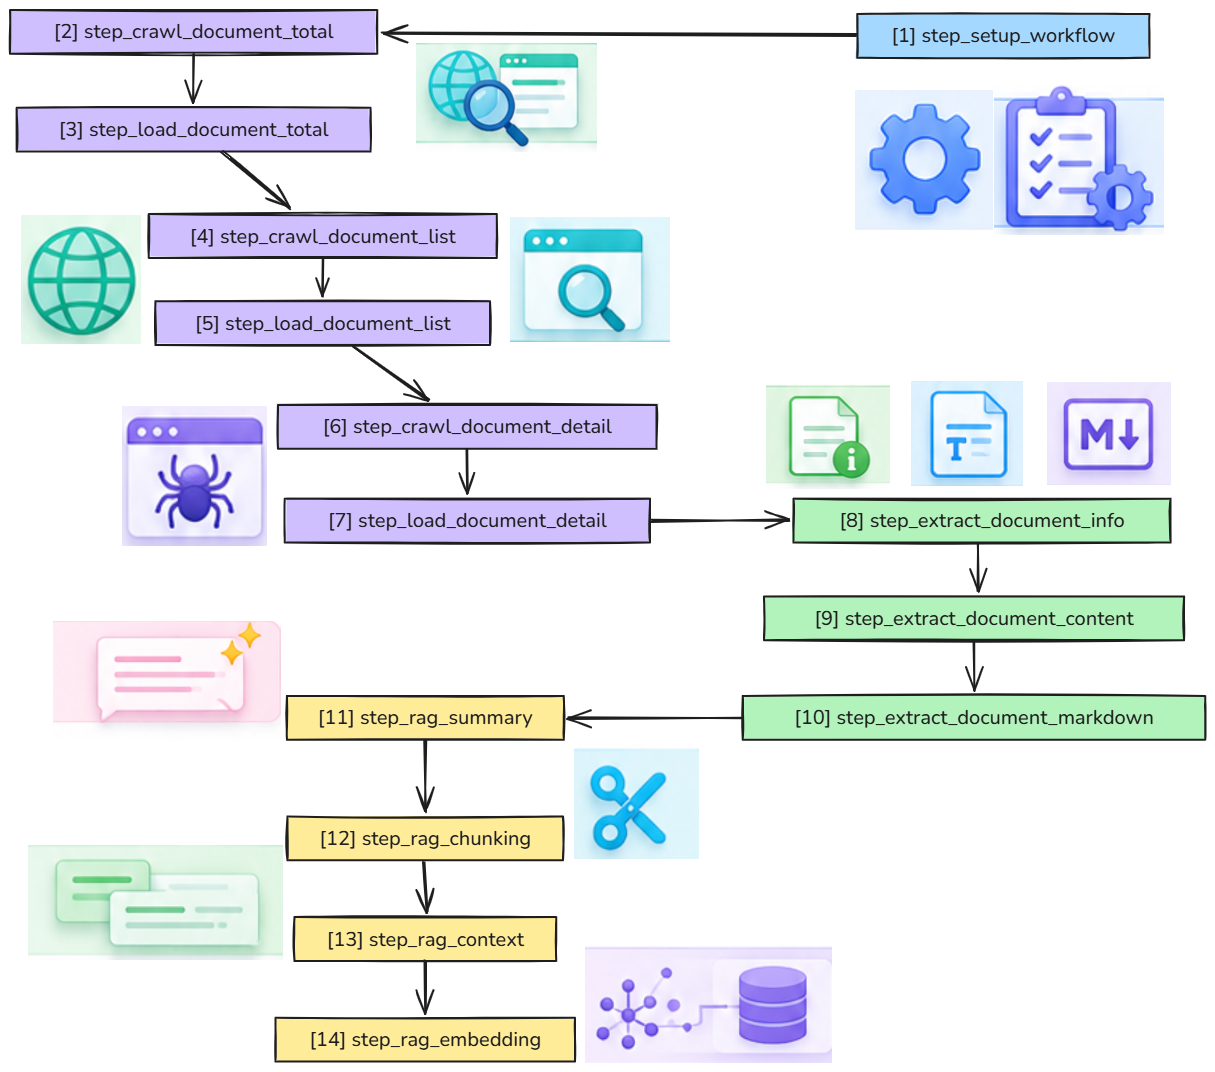
\includegraphics[height=0.55\textheight,width=0.9\textwidth,keepaspectratio]{pictures/step0.excalidraw.png}
\caption{Sơ đồ các bước thực hiện của quy trình cũ}
\end{figure}

\note{
Sơ đồ chi tiết các bước thực hiện trong quy trình cũ của đường ống dữ liệu văn bản pháp luật.
Quy trình được chia thành 3 giai đoạn: Khởi tạo luồng công việc (\texttt{step\_setup\_workflow}), thu thập tổng số lượng tài liệu (\texttt{step\_crawl\_document\_total}), tải nội dung chi tiết và cuối cùng là xử lý định dạng văn bản để chuẩn bị cho việc trích xuất thông tin.
}
\end{frame}

% % % \begin{frame}{Các bước trong đường ống dữ liệu VBPL mới}
\begin{figure}[H]
\centering
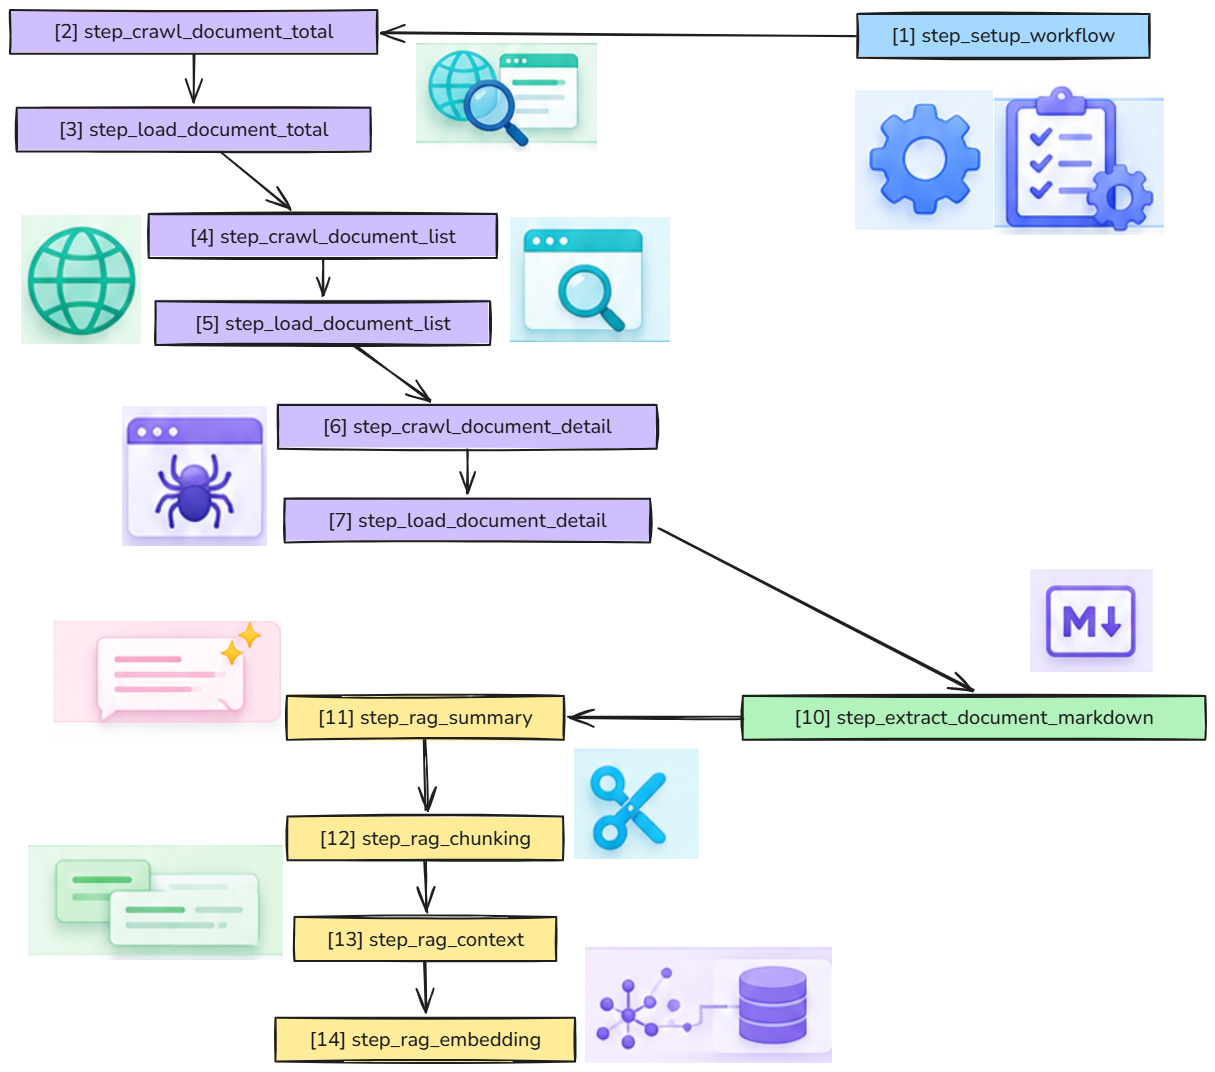
\includegraphics[height=0.7\textheight,width=0.9\textwidth,keepaspectratio]{pictures/step1.excalidraw.png}
\caption{Sơ đồ các bước thực hiện của quy trình mới}
\end{figure}

\note{
do api => bỏ bước

Sơ đồ các bước thực hiện của quy trình mới
}
\end{frame}

% % % \begin{frame}{Đường ống dữ liệu Pháp Điển}
\begin{figure}[H]
\centering
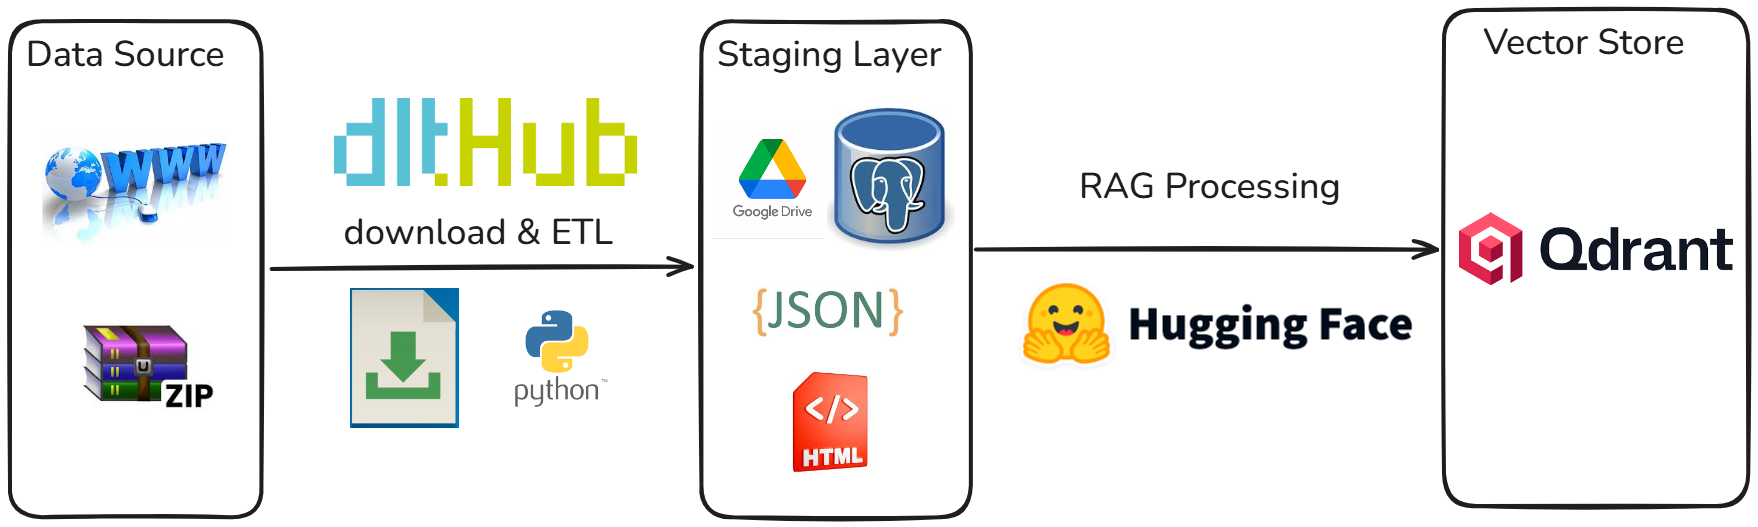
\includegraphics[height=0.55\textheight,width=0.9\textwidth,keepaspectratio]{pictures/Data-Pipeline-PhapDien.excalidraw.png}
\caption{Sơ đồ tổng quan đường ống dữ liệu Pháp Điển}
\end{figure}

\note{
Bên cạnh VBPL, hệ thống còn tích hợp Bộ Pháp Điển Việt Nam. Sơ đồ này mô tả đường ống dữ liệu Pháp Điển.
Dữ liệu Pháp Điển được tải về dưới dạng file nén ZIP từ Cổng thông tin điện tử Pháp Điển, sau đó được giải nén, chuyển đổi cấu trúc cây đề mục sang định dạng JSON, tải lên lưu trữ trên Google Drive và thực hiện vector hóa để lưu vào Vector Database.
}
\end{frame}

% % % \begin{frame}{Các bước trong đường ống dữ liệu Pháp Điển}

\begin{figure}[H]
\centering
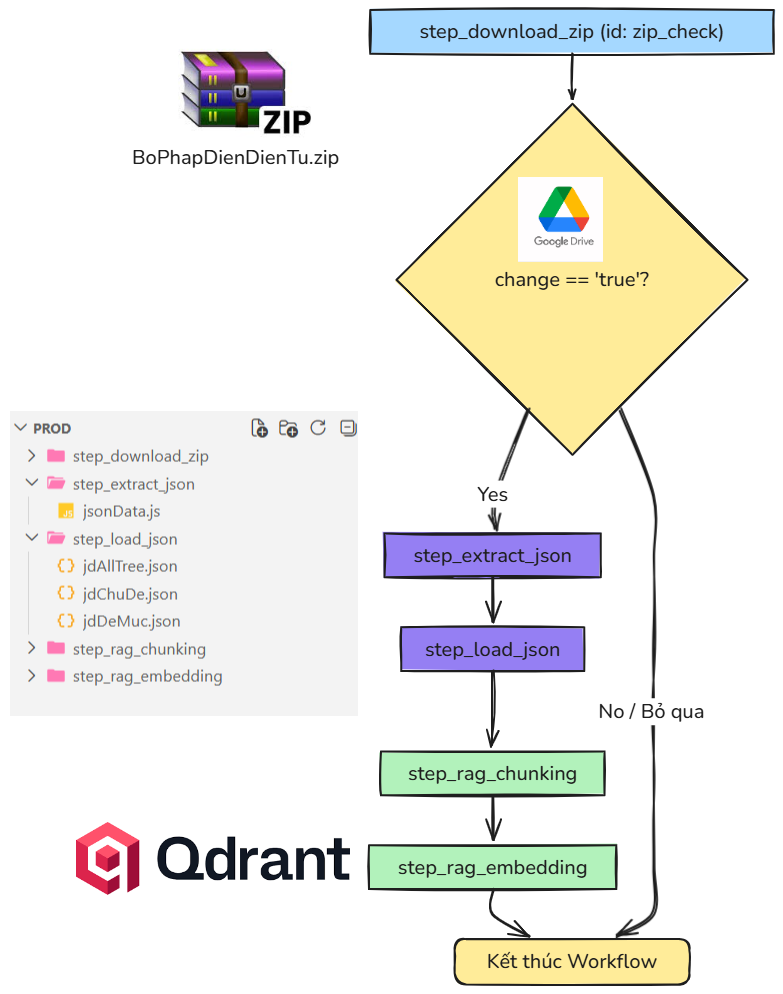
\includegraphics[height=0.7\textheight,width=0.9\textwidth,keepaspectratio]{pictures/step3.excalidraw.png}
\caption{Sơ đồ các bước thực hiện của đường ống dữ liệu Pháp Điển}
\end{figure}

\note{
Sơ đồ mô tả quy trình từng bước của đường ống dữ liệu Pháp Điển.
Quy trình bắt đầu từ việc tải file ZIP tự động (\texttt{step\_download\_zip}), tính toán mã băm MD5 để kiểm tra sự thay đổi dữ liệu so với phiên bản trước, giải nén và trích xuất cấu trúc đề mục ra các file JSON riêng biệt, sau đó chạy các tác vụ phân tích cấu trúc và lưu kết quả vector hóa.
}
\end{frame}


% % % \subsection{Agentic RAG với LangGraph}

% % % \begin{frame}{Kiến trúc Agentic RAG bằng LangGraph}
\begin{figure}[H]
\centering
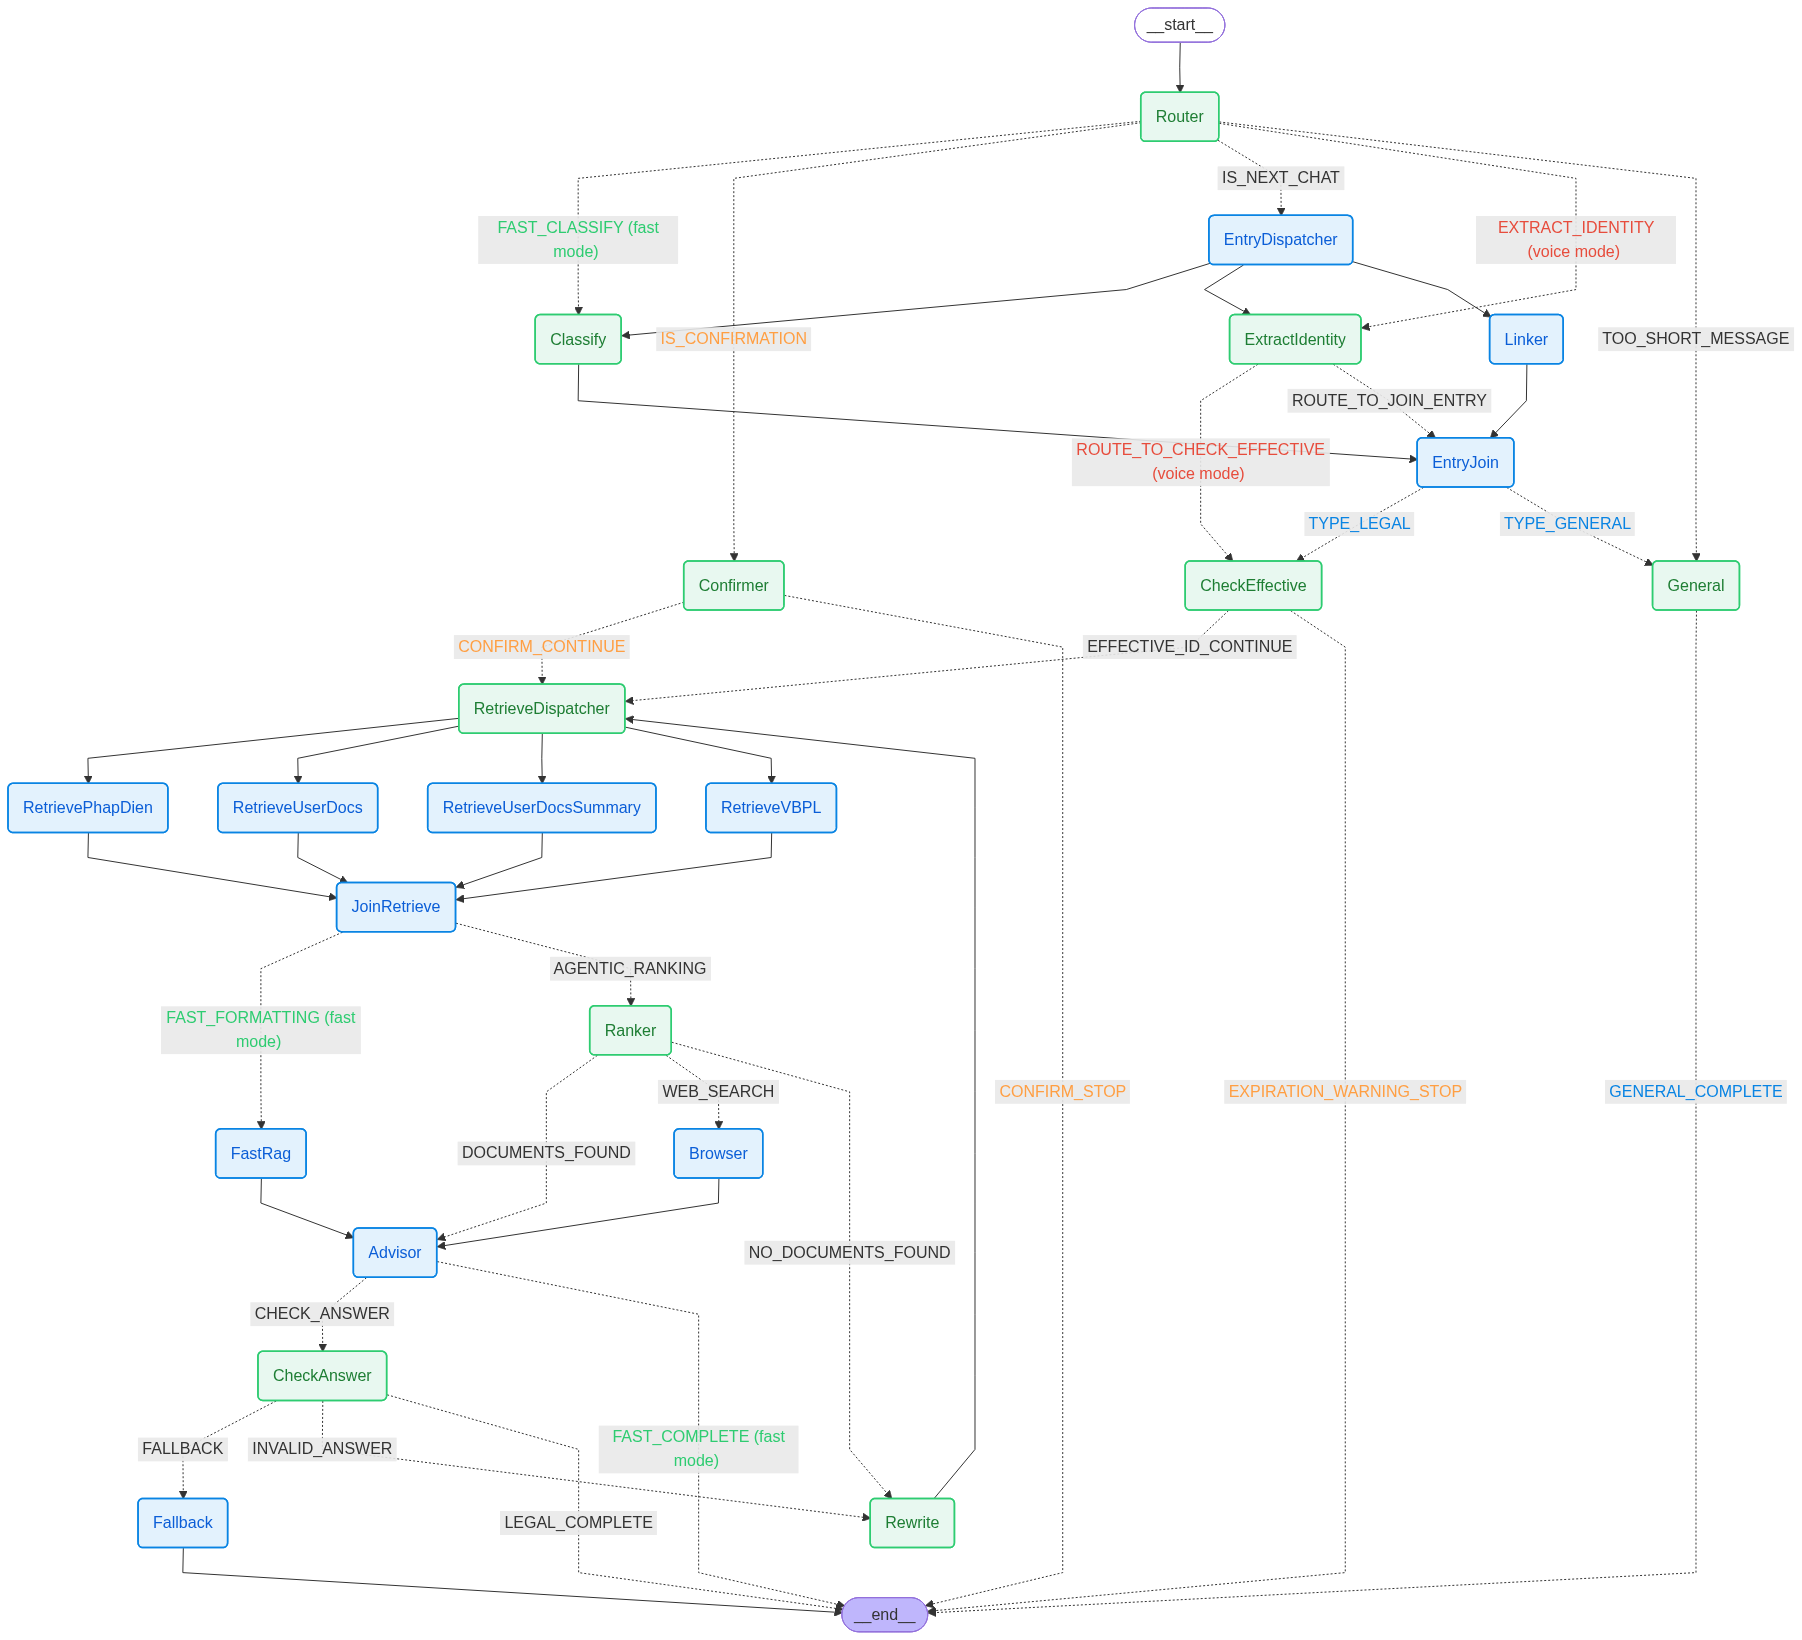
\includegraphics[height=0.55\textheight,width=0.9\textwidth,keepaspectratio]{pictures/rag_diagram.png}
\caption{Sơ đồ LangGraph của dự án}
\end{figure}

\note{
Đây là sơ đồ Agentic RAG của dự án được xây dựng bằng LangGraph. Hệ thống phân chia thông minh giữa mô hình nhỏ cho luồng cơ bản (màu xanh lá) và mô hình lớn cho các tác vụ suy luận phức tạp (màu xanh dương) để tối ưu chi phí và độ trễ.
Mỗi tin nhắn đi qua Router để kiểm tra điều kiện và định tuyến qua các node như rewrite query, retrieve tài liệu và sinh câu trả lời.
}
\end{frame}


% % % \begin{frame}{Tổng quan các dịch vụ}
\begin{figure}[H]
\centering
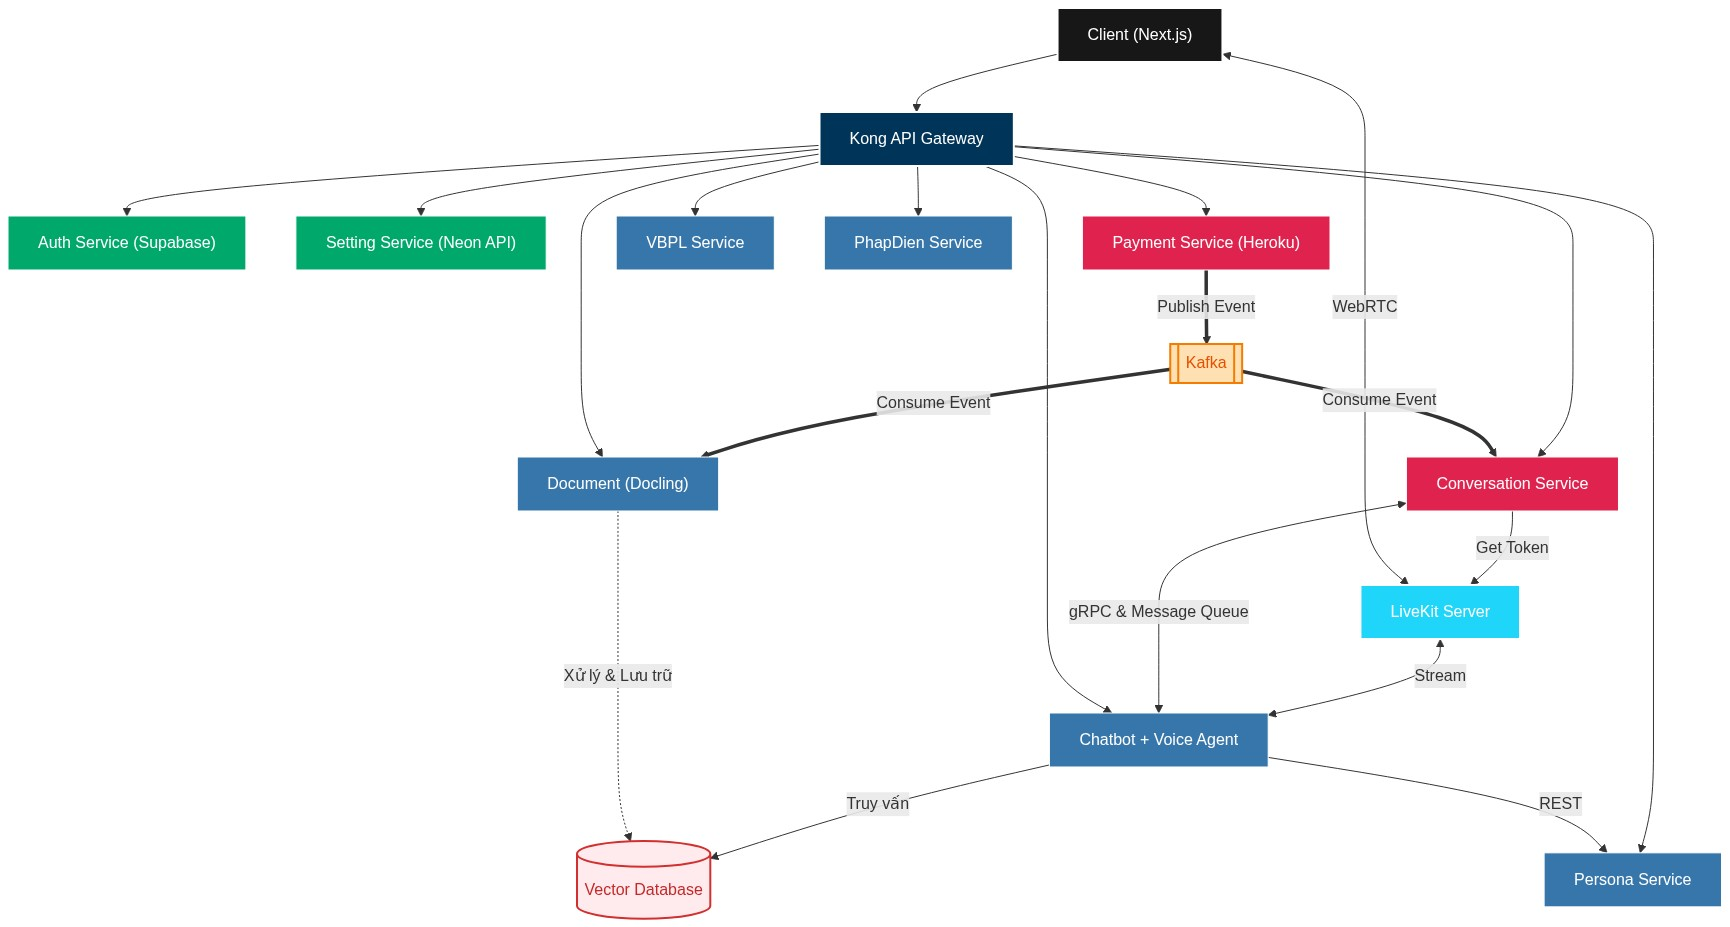
\includegraphics[height=0.7\textheight,width=0.9\textwidth,keepaspectratio]{pictures/MSA.png}
\caption{Tổng quan các dịch vụ của dự án}
\end{figure}

\note{
Sơ đồ tổng quan về kiến trúc các vi dịch vụ được triển khai trong dự án này.
Hệ thống được chia thành nhiều dịch vụ chuyên biệt như: Auth Service (xác thực), Document Service (quản lý tài liệu), Conversation Service (quản lý trò chuyện), Chatbot Service (trí tuệ nhân tạo) và Payment Service (thanh toán). Các dịch vụ này giao tiếp với nhau qua gRPC, REST API hoặc thông điệp bất đồng bộ qua Kafka/RabbitMQ.
}
\end{frame}
% nếu python cash => thanh toán , đăng nhập vẫn không sao

% Nếu các Microservice luôn để xuống service thanh toán


% % \section{Chi tiết các dịch vụ}

% % \begin{frame}{Kiến trúc Dịch vụ Thanh toán (Payment Service)}
\begin{figure}[H]
\centering
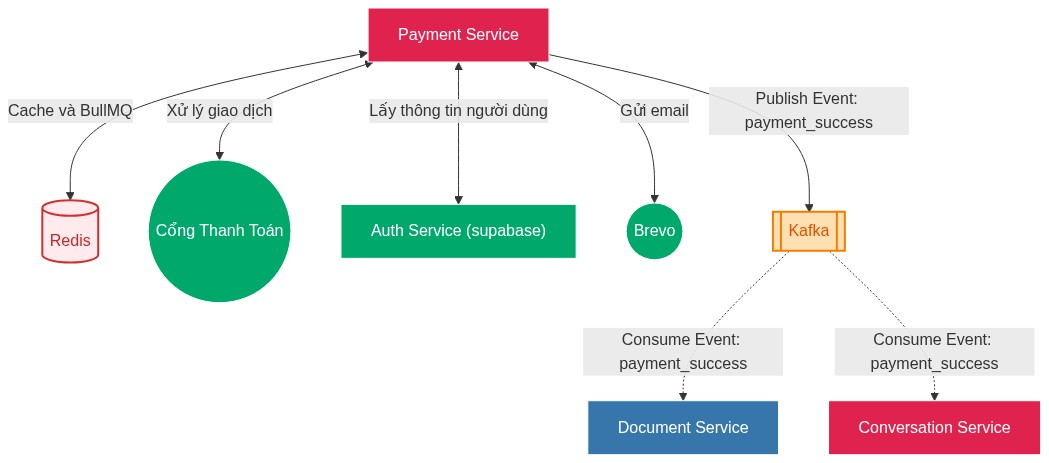
\includegraphics[height=0.7\textheight,width=0.9\textwidth,keepaspectratio]{pictures/payment-kafka-event.png}
\caption{Sơ đồ tổng quan dịch vụ thanh toán}
\end{figure}

\note{
Dịch vụ thanh toán (Payment Service) chịu trách nhiệm quản lý thông tin các gói dịch vụ (Plans), quản lý thuê bao người dùng (Subscriptions) và tích hợp với cổng thanh toán ngoại vi.
Khi người dùng thực hiện thanh toán thành công, dịch vụ này sẽ phát đi sự kiện \texttt{payment\_success} vào hệ thống truyền tin nhắn Kafka để các dịch vụ khác như Chatbot và Document cập nhật quyền VIP cho người dùng.
}
\end{frame}


% % \begin{frame}{Dịch vụ Tài liệu (Document Service)}
\begin{figure}[H]
\centering
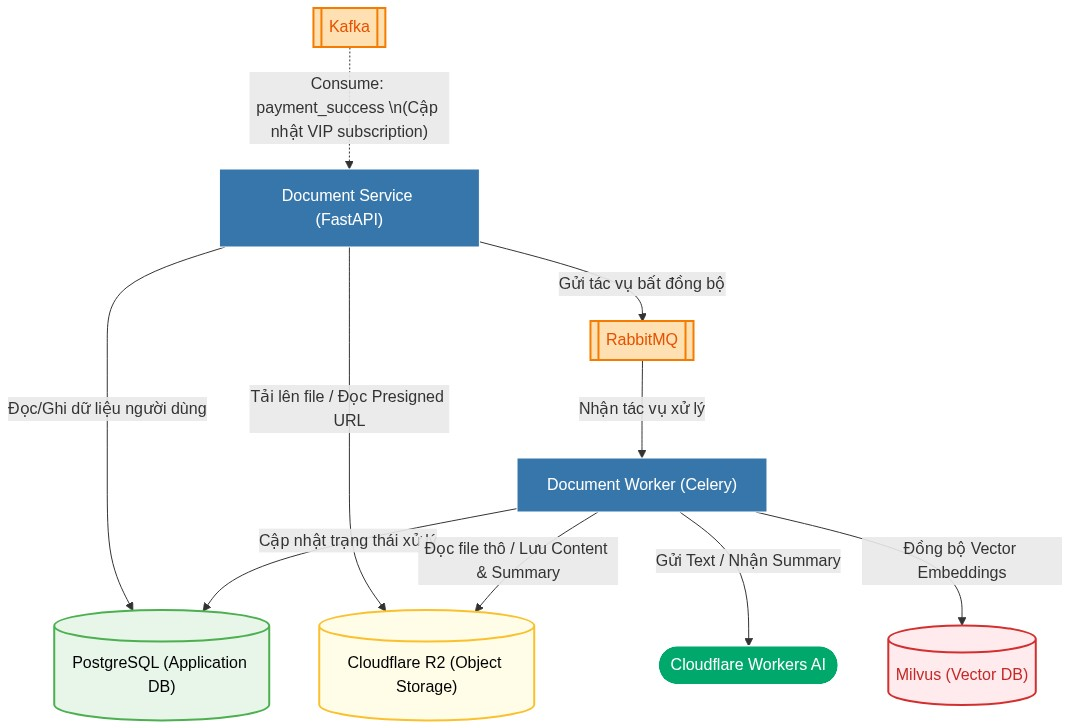
\includegraphics[height=0.7\textheight,width=0.9\textwidth,keepaspectratio]{pictures/document-overview.png}
\caption{Sơ đồ tổng quan dịch vụ văn bản}
\end{figure}

\note{
Dịch vụ tài liệu (Document Service) tiếp nhận, lưu trữ và quản lý tài liệu do người dùng VIP tải lên.
Khi nhận được tệp tin (PDF, DOCX), dịch vụ sẽ gửi yêu cầu xử lý bất đồng bộ thông qua RabbitMQ tới Document Worker. Tài liệu sẽ được trích xuất nội dung sang định dạng Markdown, tự động tóm tắt nội dung chính và tiến hành vector hóa để lưu trữ vào Vector Database Milvus phục vụ cho việc hỏi đáp trên tài liệu.
}
\end{frame}


% % \begin{frame}{Dịch vụ Chatbot và Trò chuyện}
\begin{figure}[H]
\centering
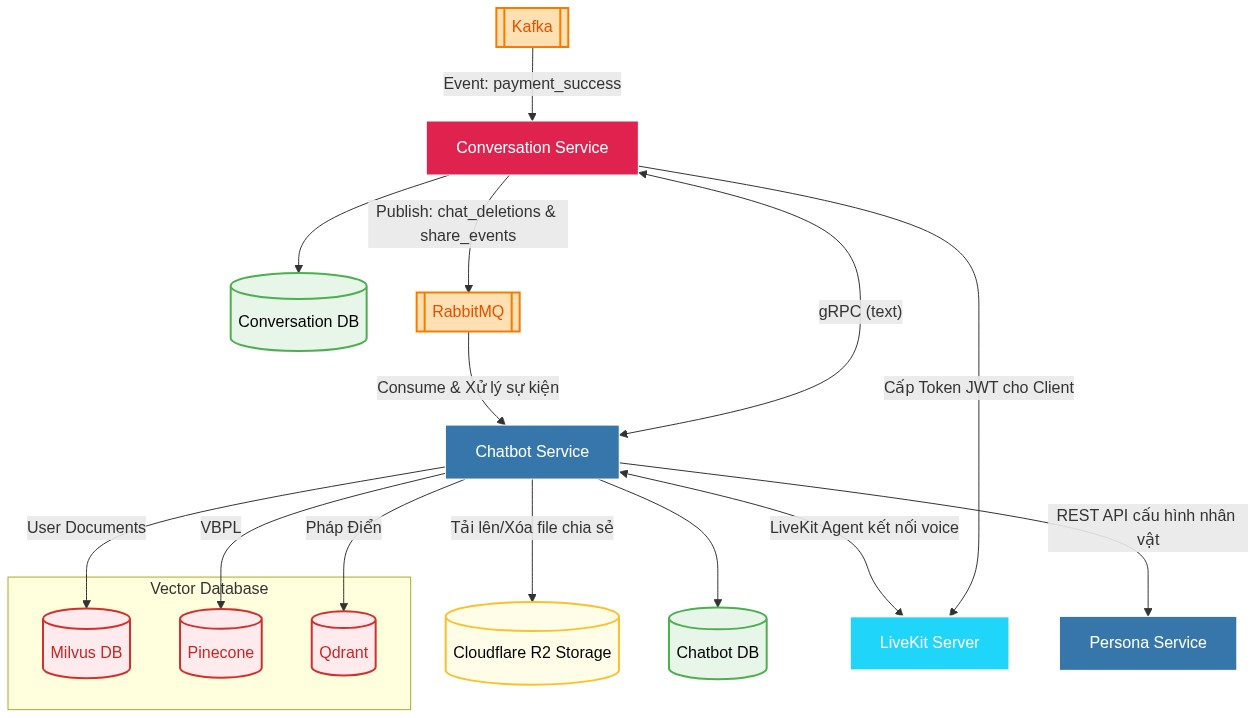
\includegraphics[height=0.7\textheight,width=0.9\textwidth,keepaspectratio]{pictures/conversation-and-chatbot-overview.png}
\caption{Sơ đồ tổng quan dịch vụ trò chuyện và dịch vụ chatbot}
\end{figure}

\note{
Sơ đồ mối quan hệ giữa Dịch vụ trò chuyện (NestJS) và Dịch vụ chatbot (Python).
Dịch vụ trò chuyện chịu trách nhiệm quản lý
trò chuyện của người dùng, lưu trữ lịch sử chat, quản lý thư mục, chia sẻ trò chuyện. Khi có tin nhắn mới, dịch vụ trò chuyện sẽ gửi yêu cầu qua giao thức gRPC hiệu năng cao đến dịch vụ chatbot (Python) để xử lý logic Agentic RAG và trả về câu trả lời dưới dạng stream.
}
\end{frame}


% % \begin{frame}{Kiến trúc tích hợp đàm thoại thời gian thực (Voice Agent)}
\begin{figure}[H]
\centering
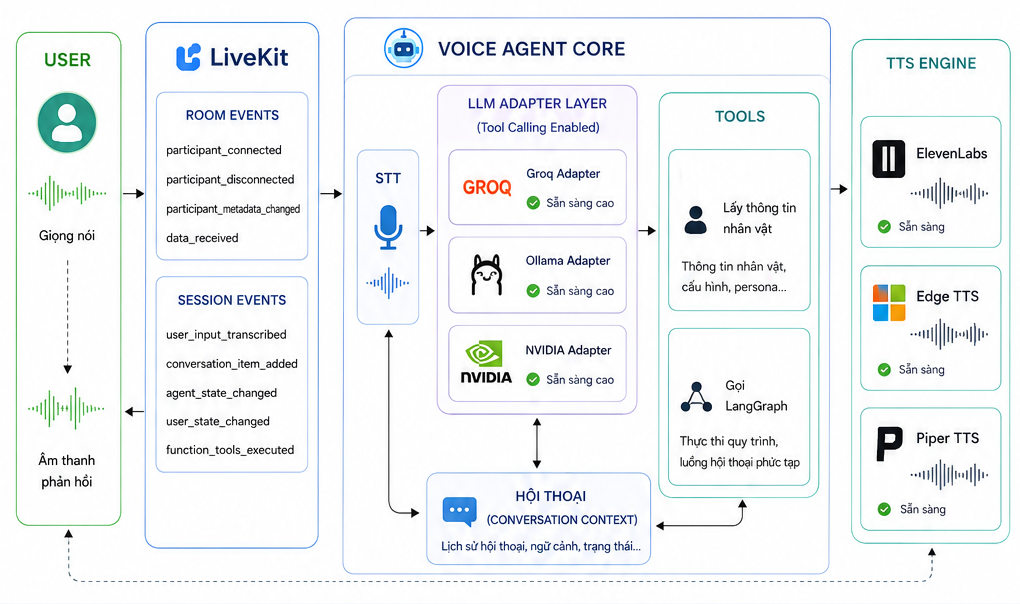
\includegraphics[height=0.7\textheight,width=0.9\textwidth,keepaspectratio]{pictures/voice-livekit-overview.png}
\caption{Sơ đồ tích hợp LiveKit đàm thoại giọng nói}
\end{figure}

\note{
Hệ thống tích hợp máy chủ LiveKit để cung cấp tính năng đàm thoại giọng nói thời gian thực với trợ lý ảo.
Khi người dùng kết nối, Voice Agent hoạt động như một LiveKit Agent, chủ động kết nối và trao đổi âm thanh hai chiều thông qua giao thức WebRTC. Voice Agent tích hợp các mô hình VAD (phát hiện giọng nói), STT (chuyển giọng nói thành văn bản), LLM (suy luận phản hồi) và TTS (chuyển văn bản thành giọng nói) với độ trễ cực thấp.
}
\end{frame}


% \ifdev
% \begin{frame}
\frametitle{}
\maketitle
\end{frame}

\begin{frame}{Cảm ơn}
\centering
\Huge{Thanks for listening!}
\end{frame}

\begin{frame}{Cảm ơn}
\centering
\Huge{Thanks for listening!}
\end{frame}

% \fi

\section{Các công nghệ khác}

\input{contents/Quy_trinh_tu_dong_hoa_CICD_bang_GitHub_Actions}
\begin{frame}{Quản lý Hạ tầng dưới dạng mã}
\begin{figure}[H]
\centering
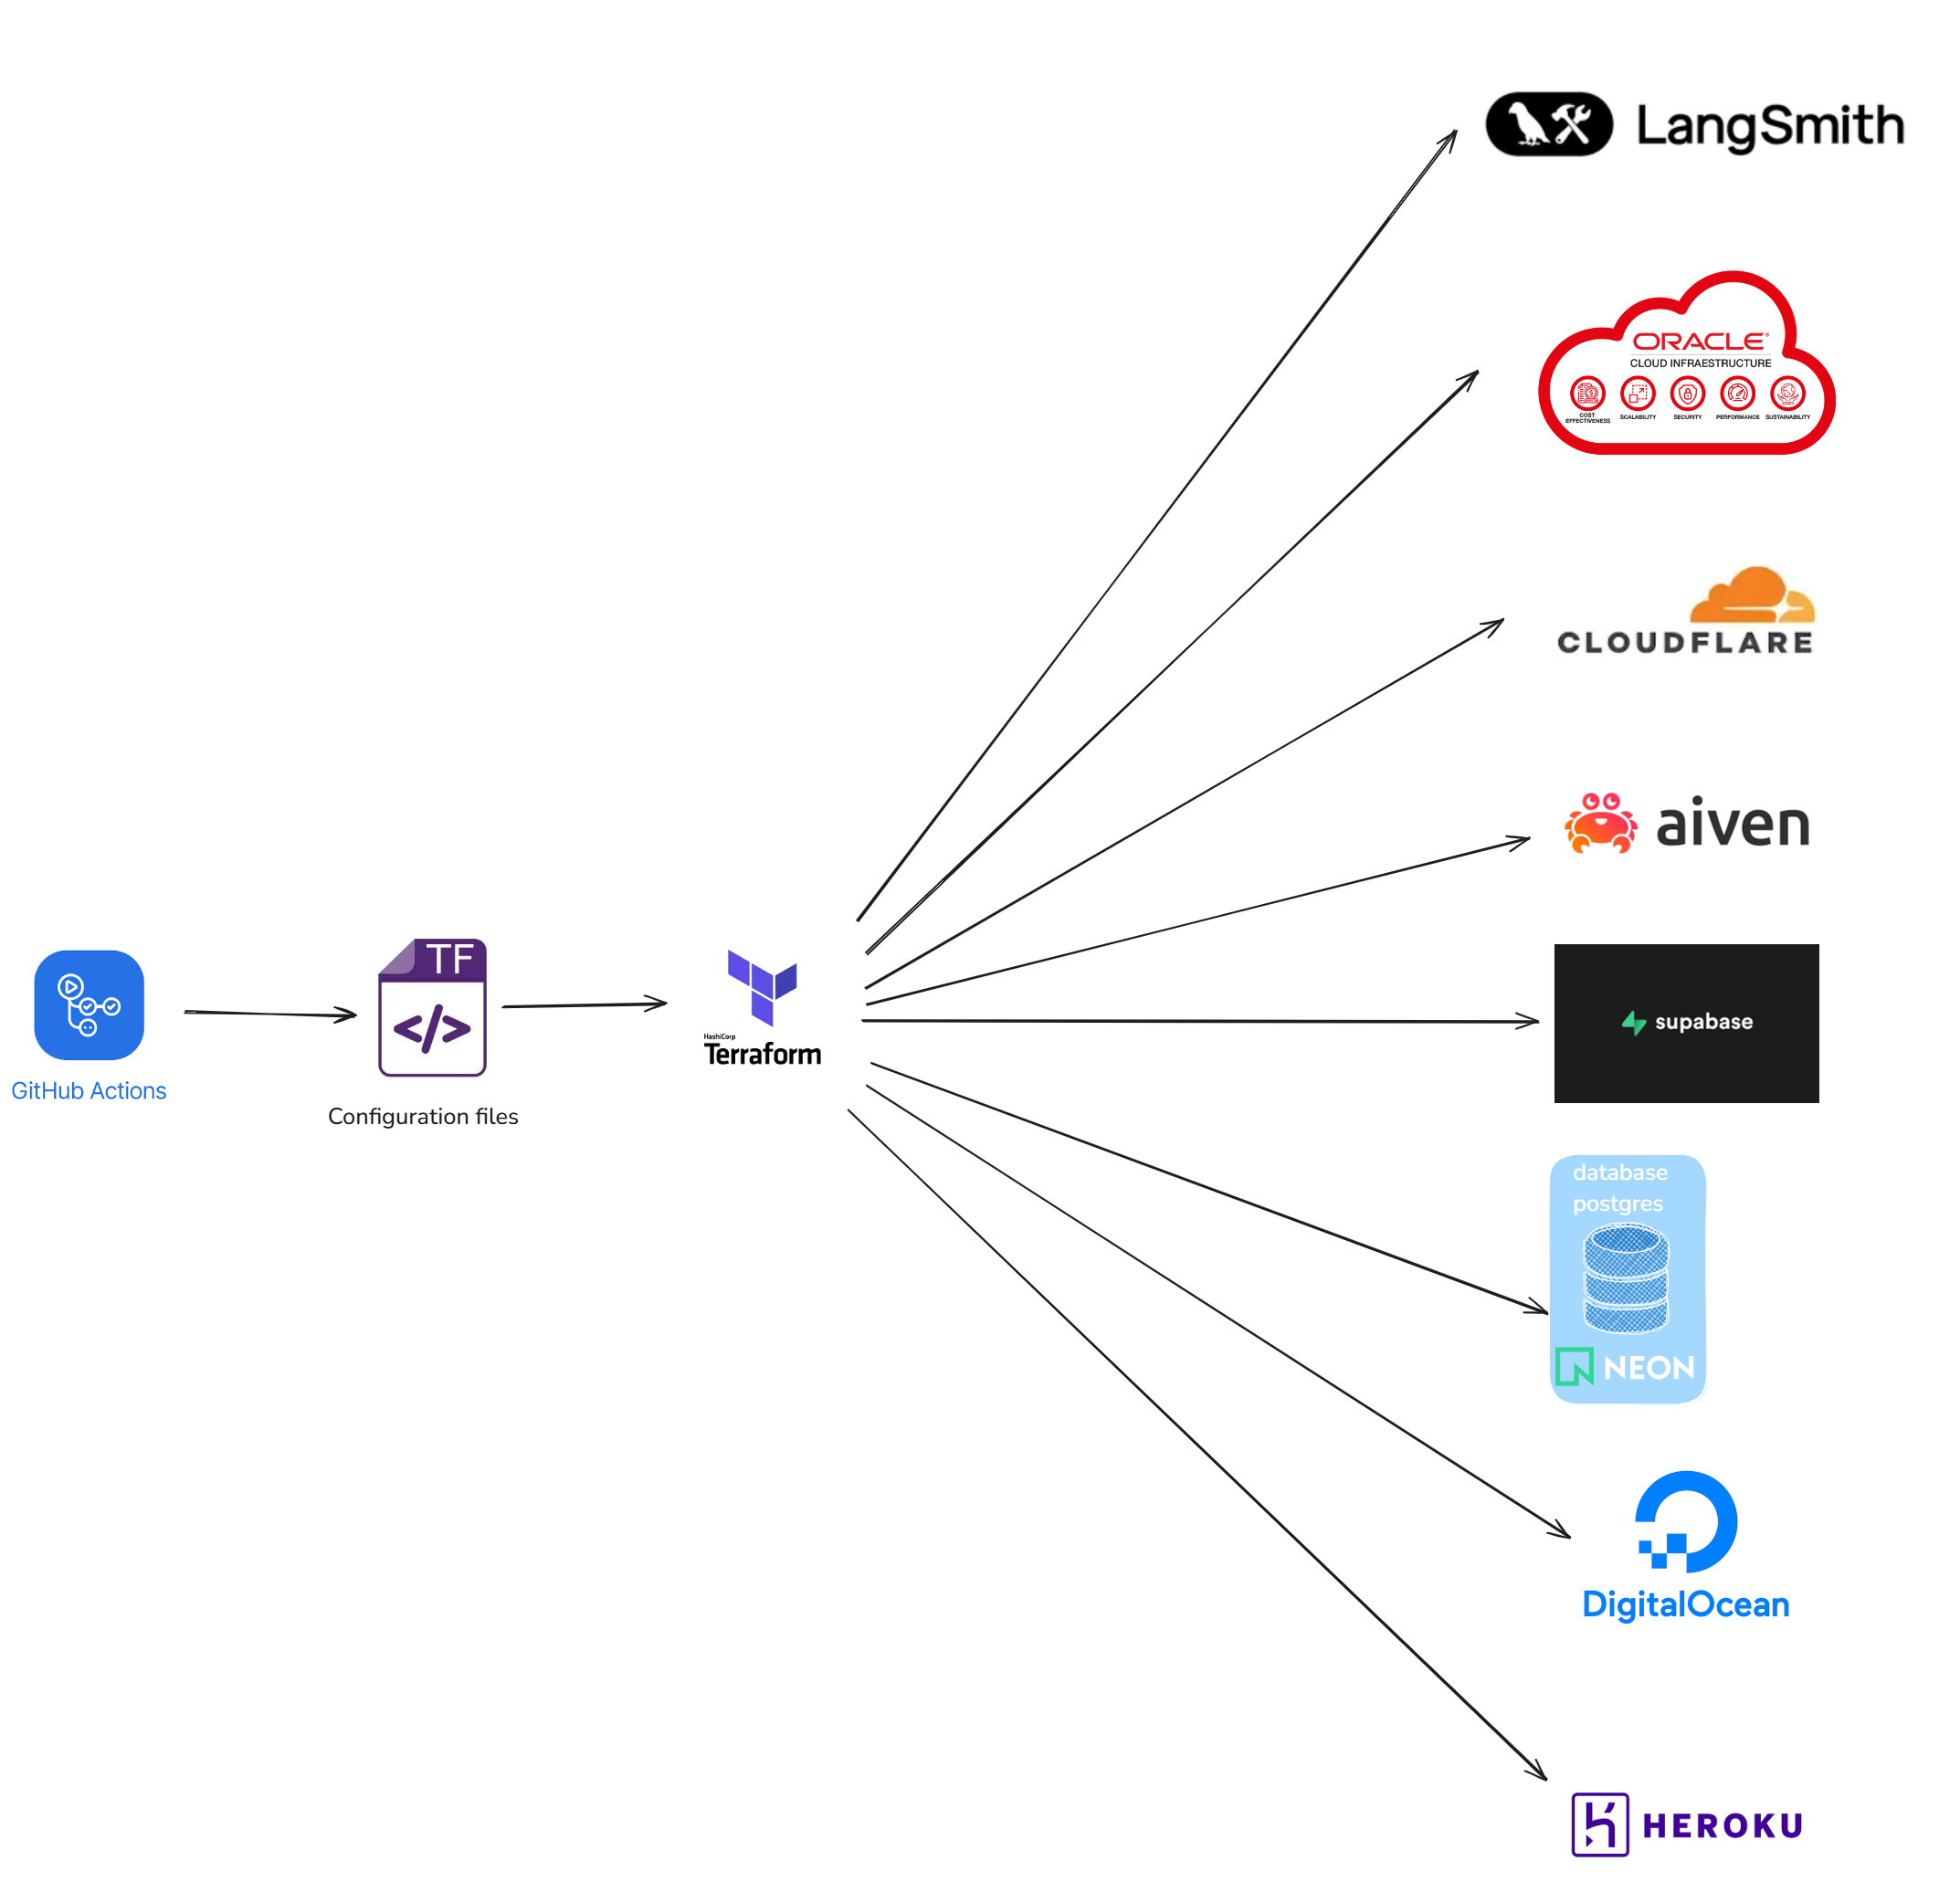
\includegraphics[height=0.7\textheight,width=0.9\textwidth,keepaspectratio]{pictures/infrastructure-as-code-IaC-terraform.excalidraw.png}
\caption{Sơ đồ tổng quan quản lý hạ tầng bằng Terraform trong dự án}
\end{figure}

\note{
Để quản lý hạ tầng một cách nhất quán và tự động, dự án sử dụng Terraform dưới dạng Infrastructure as Code (IaC).
Terraform tự động khởi tạo và cấu hình các tài nguyên bên thứ ba như: Supabase (Auth), LangSmith (giám sát RAG), Cloudflare (DNS và R2 Storage), Neon (PostgreSQL cho các vi dịch vụ), DigitalOcean (Crawl DB) và Heroku (Payment Service). Trạng thái hạ tầng được lưu trữ tập trung trên Terraform Cloud.
}
\end{frame}

\input{contents/Cau_hinh_Kong_API_Gateway_bang_Declarative_Configuration}
\begin{frame}{Kết quả Docker Image trên Docker Hub}
\begin{figure}[H]
\centering
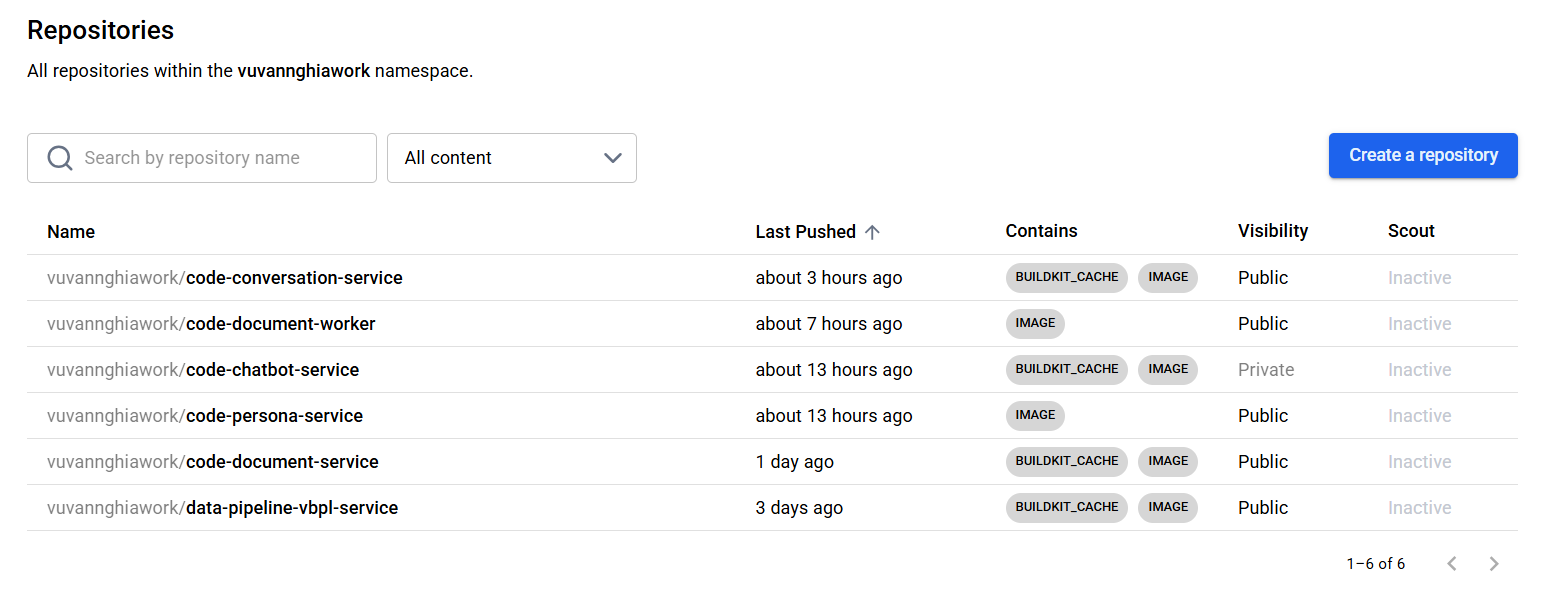
\includegraphics[height=0.55\textheight,width=0.9\textwidth,keepaspectratio]{pictures/docker-hub-web-ui2.png}
\caption{Kết quả Docker Image được push lên Docker Hub}
% \caption{Kết quả giao diện docker}
\end{figure}

\note{
docker
}
\end{frame}

\begin{frame}{Cấu hình tài nguyên Kubernetes trong GitOps Repository}
\begin{figure}[H]
\centering
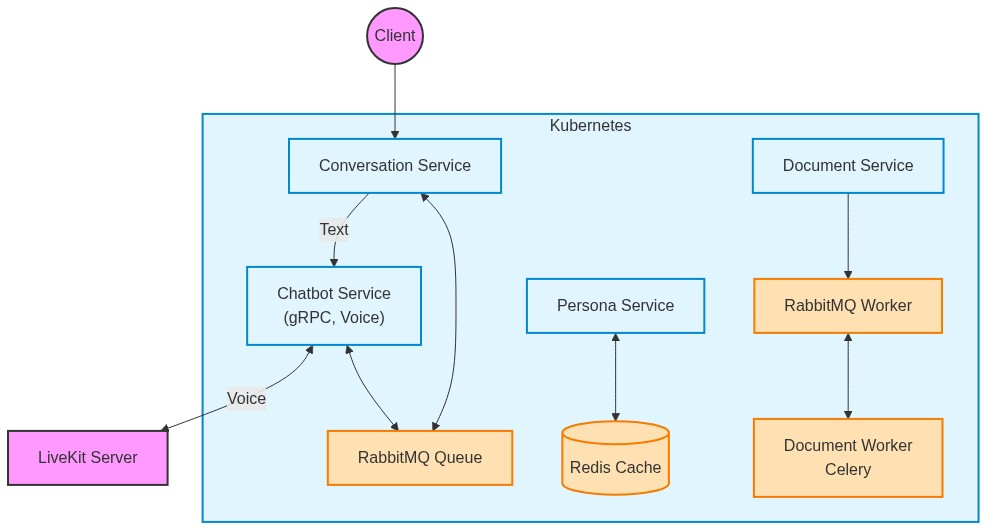
\includegraphics[height=0.55\textheight,width=0.9\textwidth,keepaspectratio]{pictures/Kubernetes.png}
\caption{Cấu hình Kubernetes trong kho lưu trữ GitOps của dự án}
\end{figure}

\note{
Đây là cấu trúc thư mục chứa các file cấu hình Kubernetes (YAML) trong kho lưu trữ GitOps của dự án.
Các dịch vụ nội bộ như RabbitMQ, Redis được chạy trực tiếp trong cụm để giảm độ trễ và được cấu hình dưới dạng ClusterIP để tăng tính bảo mật, ngăn chặn các truy cập trực tiếp từ internet. Các dịch vụ chạy bất đồng bộ như Voice Agent hay Document Worker cũng không công khai service ra bên ngoài.
}
\end{frame}


\begin{frame}{Giao diện quản lý GitOps bằng ArgoCD}
\begin{figure}[H]
\centering
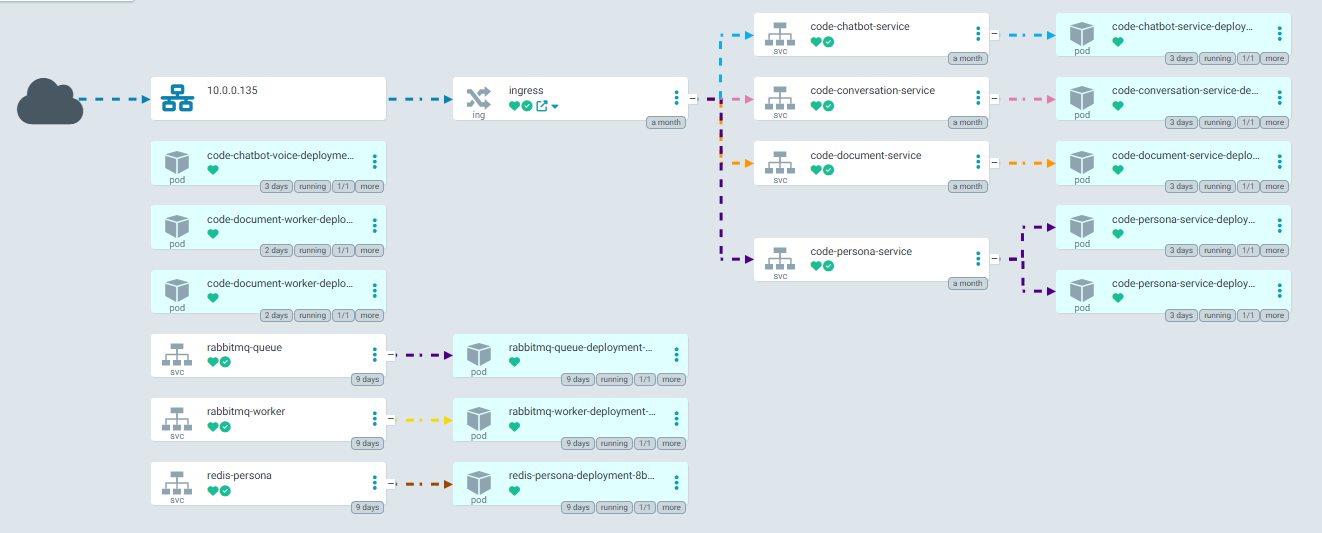
\includegraphics[height=0.55\textheight,width=0.9\textwidth,keepaspectratio]{pictures/argocd-web-ui.png}
\caption{Kết quả giao diện ArgoCD chạy docker trong kubernetes}
\end{figure}

\note{
ArgoCD được triển khai trong cụm Kubernetes để thực hiện quy trình Continuous Delivery (CD) theo mô hình GitOps.
ArgoCD liên tục giám sát kho lưu trữ Git chứa các file cấu hình Kubernetes. Khi phát hiện có sự thay đổi (ví dụ: phiên bản Docker image mới), ArgoCD sẽ tự động đồng bộ (sync) và cập nhật các Pod đang chạy trên Kubernetes thực tế để khớp với cấu hình được khai báo trên Git.
}
\end{frame}


%%%%%%%%%%%%%%%%%%%%%%%%%%%%%%%%%%%%%%%%%%%%%%%%%%%%%%%
\newpage
\phantomsection
{\centering \section*{KẾT LUẬN}}
\addcontentsline{toc}{section}{KẾT LUẬN}

\subsection*{Kết luận}

Sau thời gian nghiên cứu,
thiết kế và phát triển,
đồ án tốt nghiệp
đã hoàn thành đầy đủ các mục tiêu đề ra ban đầu,
đáp ứng toàn bộ các yêu cầu kỹ thuật
và nghiệp vụ được giao.

Về kết quả đạt được, đồ án đã mang lại các giá trị cụ thể như sau:

\begin{itemize}
\item \textbf{Về mặt sản phẩm:}
Xây dựng thành công một hệ thống trợ lý pháp luật hoàn chỉnh
hoạt động dựa trên kiến trúc vi dịch vụ
ổn định và dễ mở rộng.
Trợ lý AI sử dụng giải pháp Agentic RAG tiên tiến với LangGraph,
cho phép trả lời các truy vấn pháp lý tiếng Việt một cách chính xác,
minh bạch qua luồng suy luận rõ ràng và dẫn nguồn từ CSDL pháp điển cũng như văn bản quy phạm pháp luật chính thống.
Đồng thời, hệ thống hỗ trợ đàm thoại giọng nói thời gian thực, xử lý tài liệu người dùng và tự động hóa quy trình thanh toán.

\item \textbf{Về mặt công nghệ:}
Tích hợp và làm chủ nhiều giải pháp công nghệ hiện đại:
xây dựng hệ thống trên nền tảng kiến trúc vi dịch vụ
có ứng dụng Domain-Driven Design,
vận hành qua Kong API Gateway
với các giao thức giao tiếp REST, gRPC
cùng hệ thống hàng đợi RabbitMQ, Kafka.
Thiết lập lưu trữ đa dạng sử dụng postgres
kết hợp các CSDL vector (Qdrant, Pinecone, Milvus)
cùng các kho lưu trữ Supabase Storage, Cloudflare R2, Google Drive.
Xây dựng các đường ống thu thập dữ liệu
tự động nhờ cron-job.org, GitHub Actions, Scrapy và dlt.
Triển khai giải pháp Agentic RAG nâng cao bằng LangGraph
kết hợp các mô hình ngôn ngữ lớn
và HuggingFace (vietnamese-sbert).
Tích hợp hệ thống xác thực bảo mật qua Supabase (JWT, Google OAuth, 2FA/TOTP)
cùng phân hệ đàm thoại giọng nói LiveKit
và các công cụ TTS (edge-tts, piper-tts, ElevenLabs).
Toàn bộ hệ thống được đóng gói bằng Docker,
điều phối vận hành trên Kubernetes
thông qua quy trình CI/CD của GitHub Actions
và đồng bộ hóa hạ tầng tự động theo mô hình GitOps với ArgoCD.

\item \textbf{Về mặt kiến thức và kỹ năng tích lũy:}
Qua quá trình thực hiện đồ án,
sinh viên đã tích lũy được nhiều kiến thức
về
mô hình ngôn ngữ lớn,
kiến trúc hệ thống phân tán
và quy trình vận hành DevOps/GitOps.
Đồng thời, sinh viên phát triển
và nâng cao các kỹ năng như:
kỹ năng nghiên cứu khoa học,
tìm kiếm và tổng hợp tài liệu,
kỹ năng lập kế hoạch và quản lý dự án.

\end{itemize}

Về mặt đánh giá,
hệ thống cho thấy tính thực tiễn
khi giải quyết được bài toán tra cứu
thông tin pháp luật phức tạp.
Tuy nhiên, tính chính xác của câu trả lời phụ thuộc nhiều
vào chất lượng và độ cập nhật của CSDL nguồn.
Các mô hình AI vẫn đóng vai trò
là một trợ lý hỗ trợ đắc lực
và không thể thay thế hoàn toàn vai trò của các chuyên gia pháp lý
trong các tình huống quyết định mang tính pháp lý cao.

\subsection*{Hướng phát triển}

Để hoàn thiện ứng dụng
và nâng cao khả năng
phục vụ người dùng trong thực tế,
hướng phát triển của đồ án
trong tương lai tập trung vào các nội dung sau:

\begin{itemize}

\item \textbf{Nâng cao chất lượng AI và tối ưu hóa hệ thống RAG:}
Nghiên cứu
huấn luyện tinh chỉnh
mô hình ngôn ngữ lớn
trên các tập dữ liệu đặc thù của pháp luật Việt Nam
để nâng cao độ chính xác
và khả năng lập luận chuyên sâu.

\item \textbf{Nâng cấp khả năng điều phối luồng dữ liệu:}
Tích hợp Airflow vào quy trình xử lý dữ liệu
để tự động hóa và giám sát đường ống dữ liệu.
Sử dụng đồ thị định hướng không chu trình
(Directed Acyclic Graph - DAG)
để định nghĩa các luồng logic phức tạp dựa trên điều kiện thực tế của dữ liệu.

\item \textbf{Đánh giá và kiểm soát chất lượng mô hình AI:}
Ứng dụng khung đánh giá RAGAS
(Retrieval Augmented Generation Assessment)
để đo lường các chỉ số chất lượng của hệ thống RAG.
Từ đó, tiến hành tinh chỉnh và cấu hình các ngưỡng phản hồi
hợp lý nhằm đảm bảo tính an toàn,
chính xác và đáng tin cậy của mô hình
trước khi trả về kết quả cho người dùng.

\item \textbf{Đảm bảo chất lượng phần mềm:}
Triển khai công cụ Playwright
để xây dựng các kịch bản kiểm thử tự động
toàn diện cho cả giao diện người dùng
và các API,
giúp phát hiện lỗi sớm
và đảm bảo hệ thống hoạt động ổn định.

\item \textbf{Mở rộng phân hệ thanh toán và tài chính:}
Phát triển thêm tính năng xuất hóa đơn
điện tử phục vụ đối tượng khách hàng doanh nghiệp
và xây dựng chức năng mã giảm giá cần
xử lý thêm bài toán nhiều người
sử dụng mã giảm giá cùng lúc,
đồng thời tích hợp thêm cổng thanh toán Stripe
nhằm đáp ứng nhu cầu của tệp khách hàng quốc tế.

\item \textbf{Tối ưu hóa trải nghiệm đàm thoại giọng nói (Voice Bot):}
Nâng cấp các dịch vụ chuyển đổi giọng nói
cao cấp
hoặc tự triển khai các mô hình AI trên máy chủ có hỗ trợ GPU
nhằm giảm thiểu tối đa độ trễ, mang lại trải nghiệm đàm thoại mượt mà và tự nhiên cho người dùng.

\item \textbf{Nâng cao khả năng xử lý tài liệu đa định dạng:}
Tích hợp các công nghệ trích xuất thông tin
và đọc hiểu tài liệu tiên tiến
để hệ thống có thể xử lý đa dạng các định dạng tệp tin.

\item \textbf{Mở rộng và tối ưu hóa hạ tầng điện toán đám mây:}
Triển khai
trên môi trường đa cụm Kubernetes
nhằm tăng cường tính sẵn sàng,
đồng thời tối ưu hóa các quy trình tự động co giãn
giúp hệ thống vận hành ổn định trước lượng lớn người dùng truy cập đồng thời.

\item \textbf{Xây dựng hệ thống giám sát và quản lý nhật ký tập trung (Observability):}
Triển khai giải pháp giám sát toàn diện cho kiến trúc vi dịch vụ
bằng cách tích hợp Prometheus để thu thập số liệu hiệu năng (metrics)
hệ thống theo thời gian thực
và Grafana để trực quan hóa trạng thái vận hành, thiết lập các kịch bản cảnh báo tự động.
Đồng thời, ứng dụng bộ công cụ ELK Stack
(Elasticsearch, Logstash, Kibana)
làm giải pháp quản lý nhật ký (logging) tập trung,
hỗ trợ thu thập, tiền xử lý và phân tích log
từ tất cả các vi dịch vụ, từ đó tối ưu hóa quy trình
định vị sự cố (troubleshooting) và đảm bảo tính sẵn sàng cao cho hệ thống.

\end{itemize}
\newpage

\newpage
\phantomsection
{\centering \section*{TÀI LIỆU THAM KHẢO}}
\addcontentsline{toc}{section}{TÀI LIỆU THAM KHẢO}

\begingroup
\renewcommand{\section}[2]{} % Bỏ qua lệnh tạo tiêu đề tự động của thebibliography
\begin{thebibliography}{00}

\bibitem{vaswani2017attention}
Vaswani, A., Shazeer, N., Parmar, N., Uszkoreit, J., Jones, L., Gomez, A. N., Kaiser, L., \& Polosukhin, I. (2017). Attention is all you need. \textit{Advances in neural information processing systems}, 30. \url{http://arxiv.org/abs/1706.03762}

\bibitem{ARSLAN20243781}
Arslan, M., Ghanem, H., Munawar, S., \& Cruz, C. (2024). A Survey on RAG with LLMs. \textit{Procedia Computer Science}, 246, 3781-3790. \url{https://doi.org/10.1016/j.procs.2024.09.178}

\bibitem{agentic-ai-2026}
Dwivedi, Y. K., et al. (2026). Agentic AI Systems: What It Is and Isn't. \textit{Global Business and Organizational Excellence}, 45(3), 253-263. \url{https://doi.org/10.1002/joe.70018}

\bibitem{ddd-evans}
Evans, E. (2004). \textit{Domain-Driven Design: Tackling Complexity in the Heart of Software}. Addison-Wesley Professional.

\bibitem{ddd-quickly}
Marinescu, F., \& Abel, A. (2006). \textit{Domain-Driven Design Quickly}. C4Media.

\bibitem{fowler-event-driven}
Fowler, M. (2017). \textit{What do you mean by "Event-Driven"?}. Truy cập ngày 28/06/2026, từ \url{https://martinfowler.com/articles/201701-event-driven.html}

\bibitem{outbox-pattern}
Richardson, C. \textit{Pattern: Transactional outbox}. Microservices.io. Truy cập ngày 28/06/2026, từ \url{https://microservices.io/patterns/data/transactional-outbox.html}

\bibitem{aws-rag}
Amazon Web Services. \textit{Retrieval-Augmented Generation (RAG) là gì?}. Truy cập ngày 28/06/2026, từ \url{https://aws.amazon.com/vi/what-is/retrieval-augmented-generation}

\bibitem{weaviate-rag}
Weaviate. \textit{What is Agentic RAG?}. Truy cập ngày 28/06/2026, từ \url{https://weaviate.io/blog/what-is-agentic-rag}

\bibitem{dlthub}
dltHub. \textit{Introduction to dlt}. Truy cập ngày 28/06/2026, từ \url{https://dlthub.com/docs/intro}

\bibitem{scrapy}
Scrapy. \textit{A Fast and Powerful Scraping and Web Crawling Framework}. Truy cập ngày 28/06/2026, từ \url{https://www.scrapy.org}

\bibitem{vbpl}
Cơ sở dữ liệu Quốc gia về Văn bản Pháp luật. Truy cập ngày 28/06/2026, từ \url{https://vbpl.vn}

\bibitem{phapdien}
Bộ Tư pháp. \textit{Chi tiết Bộ Pháp điển}. Truy cập ngày 28/06/2026, từ \url{https://phapdien.moj.gov.vn/Pages/chi-tiet-bo-phap-dien.aspx}

\bibitem{vietnamese-sbert}
Hugging Face. \textit{vietnamese-sbert}. Truy cập ngày 28/06/2026, từ \url{https://huggingface.co/keepitreal/vietnamese-sbert}

\bibitem{langchain-vectorstores}
LangChain. \textit{Vector stores}. Truy cập ngày 28/06/2026, từ \url{https://docs.langchain.com/oss/python/integrations/vectorstores}

\bibitem{langgraph}
LangChain. \textit{LangGraph Overview}. Truy cập ngày 28/06/2026, từ \url{https://docs.langchain.com/oss/python/langgraph/overview}

\bibitem{ddd-hexagon}
Sairyss. \textit{Domain-Driven Hexagon}. GitHub. Truy cập ngày 28/06/2026, từ \url{https://github.com/Sairyss/domain-driven-hexagon#diagram}

\bibitem{doppler-branch}
Doppler. \textit{Branch Configs}. Truy cập ngày 28/06/2026, từ \url{https://docs.doppler.com/docs/branch-configs}

\bibitem{kong-gateway}
Kong. \textit{Kong Gateway}. Truy cập ngày 28/06/2026, từ \url{https://developer.konghq.com/gateway}

\bibitem{supabase-storage}
Supabase. \textit{Storage Guides}. Truy cập ngày 28/06/2026, từ \url{https://supabase.com/docs/guides/storage}

\bibitem{supabase-totp}
Supabase. \textit{Time-based One-Time Passwords (TOTP)}. Truy cập ngày 28/06/2026, từ \url{https://supabase.com/docs/guides/auth/auth-mfa/totp}

\bibitem{supabase-jwts}
Supabase. \textit{JSON Web Tokens (JWTs)}. Truy cập ngày 28/06/2026, từ \url{https://supabase.com/docs/guides/auth/jwts}

\bibitem{neon-postgrest}
Neon. \textit{Create a REST API from Postgres with PostgREST}. Truy cập ngày 28/06/2026, từ \url{https://neon.com/docs/guides/postgrest}

\bibitem{heroku-docker}
Heroku. \textit{Deploying with Docker}. Truy cập ngày 28/06/2026, từ \url{https://devcenter.heroku.com/categories/deploying-with-docker}

\bibitem{momo-notification}
MoMo. \textit{Payment Notification}. Truy cập ngày 28/06/2026, từ \url{https://developers.momo.vn/v3/vi/docs/payment/api/result-handling/notification/}

\bibitem{nestjs-cqrs}
NestJS. \textit{CQRS}. Truy cập ngày 28/06/2026, từ \url{https://docs.nestjs.com/recipes/cqrs}

\bibitem{nestjs-sse}
NestJS. \textit{Server-Sent Events}. Truy cập ngày 28/06/2026, từ \url{https://docs.nestjs.com/techniques/server-sent-events}

\bibitem{typeorm-migrations}
TypeORM. \textit{How migrations work?}. Truy cập ngày 28/06/2026, từ \url{https://typeorm.io/docs/migrations/why}

\bibitem{alembic-autogenerate}
Alembic. \textit{Auto Generating Migrations}. Truy cập ngày 28/06/2026, từ \url{https://alembic.sqlalchemy.org/en/latest/autogenerate.html}

\bibitem{fastapi}
FastAPI. \textit{FastAPI Framework}. Truy cập ngày 28/06/2026, từ \url{https://fastapi.tiangolo.com}

\bibitem{testcontainers}
Testcontainers. \textit{Testcontainers}. Truy cập ngày 28/06/2026, từ \url{https://testcontainers.com}

\bibitem{docling}
Docling. \textit{Docling AI}. Truy cập ngày 28/06/2026, từ \url{https://www.docling.ai}

\bibitem{langfuse-langsmith}
Langfuse. \textit{LangSmith Alternative}. Truy cập ngày 28/06/2026, từ \url{https://langfuse.com/resources/engineering/langsmith-alternative}

\bibitem{bullmq}
BullMQ. \textit{BullMQ Documentation}. Truy cập ngày 28/06/2026, từ \url{https://docs.bullmq.io}

\bibitem{celeryq-rabbitmq}
Celery. \textit{Using RabbitMQ}. Truy cập ngày 28/06/2026, từ \url{https://docs.celeryq.dev/en/v5.5.3/getting-started/backends-and-brokers/rabbitmq.html}

\bibitem{rabbitmq-dlx}
RabbitMQ. \textit{Dead Letter Exchanges}. Truy cập ngày 28/06/2026, từ \url{https://www.rabbitmq.com/docs/dlx}

\bibitem{kafka-design}
Apache Kafka. \textit{Design}. Truy cập ngày 28/06/2026, từ \url{https://kafka.apache.org/43/design/design}

\bibitem{github-actions}
GitHub. \textit{GitHub Actions Documentation}. Truy cập ngày 28/06/2026, từ \url{https://docs.github.com/en/actions}

\bibitem{terraform}
HashiCorp. \textit{Terraform Documentation}. Truy cập ngày 28/06/2026, từ \url{https://developer.hashicorp.com/terraform}

\bibitem{neon-auth}
Neon. \textit{Custom Authentication Providers}. Truy cập ngày 28/06/2026, từ \url{https://neon.com/docs/data-api/custom-authentication-providers}

\bibitem{grpc-docs}
gRPC. \textit{gRPC Documentation}. Truy cập ngày 28/06/2026, từ \url{https://grpc.io/docs}

\bibitem{livekit-events}
LiveKit. \textit{Agent Events}. Truy cập ngày 28/06/2026, từ \url{https://docs.livekit.io/reference/agents/events}

\bibitem{livekit-roomevent}
LiveKit. \textit{RoomEvent Enum}. Truy cập ngày 28/06/2026, từ \url{https://docs.livekit.io/reference/client-sdk-js/enums/RoomEvent.html}

\bibitem{livekit-tracks}
LiveKit. \textit{Rooms, Participants, Tracks}. Truy cập ngày 28/06/2026, từ \url{https://docs.livekit.io/intro/basics/rooms-participants-tracks}

\bibitem{elevenlabs-intro}
ElevenLabs. \textit{Introduction to ElevenLabs}. Truy cập ngày 28/06/2026, từ \url{https://elevenlabs.io/docs/overview/intro}

\bibitem{nghitts}
nghimestudio. \textit{nghitts}. GitHub. Truy cập ngày 28/06/2026, từ \url{https://github.com/nghimestudio/nghitts}

\bibitem{vnpt-chatbot-luat}
VNPT AI. (2025). \textit{Chatbot AI tra cứu luật: Trợ lý pháp lý thông minh thời đại số}. Truy cập ngày 28/06/2026, từ \url{https://vnptai.io/vi/blog/detail/chatbot-ai-tra-cuu-luat}

\bibitem{langgraph-innovation}
Innovation Essence. \textit{'LangGraph' Allow dynamic AI assistants with context-aware}. Truy cập ngày 28/06/2026, từ \url{https://innovationessence.com/langgraph-allow-dynamic-ai-assistants-with-context-aware/}

\bibitem{vernon2013implementing}
Vernon, V. (2013). \textit{Implementing Domain-Driven Design}. Addison-Wesley Professional. Truy cập ngày 28/06/2026, từ \url{https://www.oreilly.com/library/view/implementing-domain-driven-design/9780133039900/ch02lev2sec2.html}

\bibitem{bytebytego-cicd}
ByteByteGo. \textit{A crash course in CI/CD}. Truy cập ngày 28/06/2026, từ \url{https://blog.bytebytego.com/p/a-crash-course-in-cicd}

\bibitem{vbpl-gioi-thieu}
Cơ sở dữ liệu Quốc gia về Văn bản Pháp luật. \textit{Giới thiệu}. Truy cập ngày 28/06/2026, từ \url{https://vbpl.vn/gioi-thieu}

\bibitem{dlthub-how-it-works}
dltHub. \textit{How dlt works}. Truy cập ngày 28/06/2026, từ \url{https://dlthub.com/docs/reference/explainers/how-dlt-works}

\bibitem{twilio-totp}
Twilio. \textit{Authy API and Google Authenticator}. Truy cập ngày 28/06/2026, từ \url{https://www.twilio.com/en-us/blog/developers/tutorials/product/authy-api-and-google-authenticator}

\end{thebibliography}
\endgroup

\newpage

\newpage
\phantomsection
{\centering \section*{PHỤ LỤC}}
\addcontentsline{toc}{section}{PHỤ LỤC}

% Cấu hình đánh số riêng cho hình vẽ và bảng biểu trong Phụ lục
\setcounter{figure}{0}
\renewcommand{\thefigure}{PL.\arabic{figure}}
\setcounter{table}{0}
\renewcommand{\thetable}{PL.\arabic{table}}

\subsection*{HẠN CHẾ TÀI NGUYÊN}

Là một dự án cá nhân,
hệ thống hiện tại đang gặp phải những
hạn chế
về mặt hạ tầng và chi phí tài nguyên.
Cụ thể, việc triển khai Kong API Gateway
trên nền tảng miễn phí của Render (cold start),
kết hợp với giới hạn
băng thông network của VPS
và hạn mức LLM, đã tạo ra những nút thắt cổ chai đáng kể về hiệu năng.
Việc áp dụng mẫu Outbox có ưu điểm lớn là kiến trúc đơn giản,
dễ triển khai
nhưng lại bộc lộ nhược điểm chí mạng là liên tục thực hiện truy vấn (polling) vào database ngay cả khi không có dữ liệu thay đổi.
Điều này vô tình gây áp lực cực kỳ lớn lên cấu hình phần cứng vốn đã khiêm tốn của database postgres (chạy trên cluster miễn phí của Neon).
Do phân khúc tài nguyên bị thắt chặt và hệ thống hiện tại vẫn chưa tích hợp phần kiểm thử hiệu năng (Performance Testing) để đo lường định lượng, dự án vẫn chưa thể đạt đến trạng thái tối ưu và hoạt động mượt mà như kỳ vọng.

% \subsection*{Bảng thông tin các trường hợp kịch bản}

\subsection*{TRƯỜNG HỢP KỊCH BẢN}

Dưới đây là bảng thống kê kết quả chạy thử nghiệm tự động các kịch bản
để đánh giá khả năng chống ảo giác (hallucination), độ chính xác của tài liệu truy xuất (context) và hiệu năng phản hồi (latency) của hệ thống.
Bảng dữ liệu
này
được chạy tự động
với Github Actions.

\textbf{Link:} \url{https://github.com/20206205Tech/demo/actions/runs/28315626225}

\begin{figure}[H]
\centering
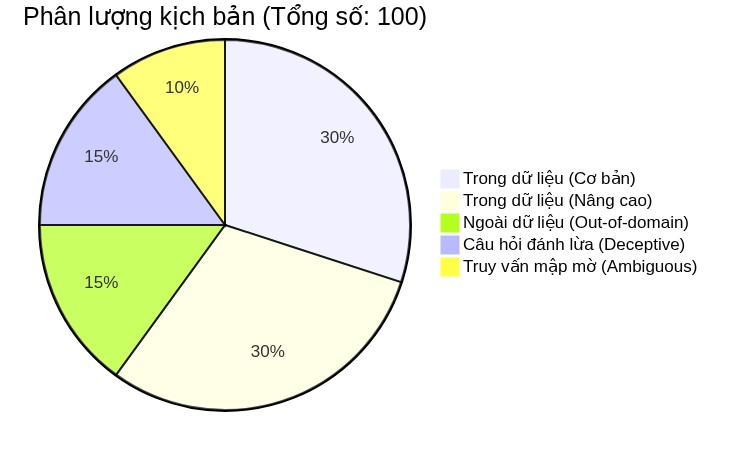
\includegraphics[width=0.85\textwidth]{contents/0/phu_luc/python/bang3.png}

\refstepcounter{figure}
\textbf{Hình \thefigure:} Biểu đồ phân lượng các kịch bản thử nghiệm hệ thống
\label{fig:ti_le_kich_ban_thu_nghiem}
\end{figure}


\begin{longtable}{|l|p{6.5cm}|c|c|}
\caption{Bảng thống kê các kịch bản thử nghiệm hệ thống} \label{tab:thong_ke_chi_tiet} \\
\hline
\makecell[l]{\textbf{Phân loại}\\\textbf{trường hợp}} & \textbf{Câu hỏi} & \makecell{\textbf{Tài liệu}\\\textbf{truy xuất}} & \textbf{Thời gian} \\ \hline
\endfirsthead
\multicolumn{4}{c}{{\bfseries Bảng \thetable{} -- Tiếp theo từ trang trước}} \\
\hline
\makecell[l]{\textbf{Phân loại}\\\textbf{trường hợp}} & \textbf{Câu hỏi} & \makecell{\textbf{Tài liệu}\\\textbf{truy xuất}} & \textbf{Thời gian} \\ \hline
\endhead
\hline
\multicolumn{4}{r}{{Tiếp tục ở trang sau}} \\
\endfoot
\hline
\endlastfoot
\makecell[l]{Trong dữ liệu\\(Cơ bản)} & Thời gian thử việc tối đa đối với người lao động có trình độ đại học là bao lâu? & 44 tài liệu & 64.58s \\ \hline
\makecell[l]{Trong dữ liệu\\(Cơ bản)} & Thời gian thử việc tối đa của lao động có trình độ cao đẳng là bao lâu? & 26 tài liệu & 25.68s \\ \hline
\makecell[l]{Trong dữ liệu\\(Cơ bản)} & Người lao động được nghỉ bao nhiêu ngày phép năm nếu làm đủ 12 tháng trong điều kiện bình thường? & 26 tài liệu & 39.67s \\ \hline
\makecell[l]{Trong dữ liệu\\(Cơ bản)} & Lương thử việc tối thiểu bằng bao nhiêu phần trăm lương của công việc đó? & 22 tài liệu & 14.22s \\ \hline
\makecell[l]{Trong dữ liệu\\(Cơ bản)} & Thời giờ làm việc bình thường không quá bao nhiêu giờ trong một ngày và một tuần? & 0 tài liệu & 1.92s \\ \hline
\makecell[l]{Trong dữ liệu\\(Cơ bản)} & Làm thêm giờ vào ngày nghỉ hằng tuần được trả lương ít nhất bằng bao nhiêu? & 0 tài liệu & 31.91s \\ \hline
\makecell[l]{Trong dữ liệu\\(Cơ bản)} & Làm thêm giờ vào ngày nghỉ lễ, tết, ngày nghỉ có hưởng lương được trả lương ít nhất bằng bao nhiêu? & 0 tài liệu & 30.08s \\ \hline
\makecell[l]{Trong dữ liệu\\(Cơ bản)} & Có bao nhiêu loại hợp đồng lao động theo Bộ luật Lao động hiện hành? & 22 tài liệu & 55.67s \\ \hline
\makecell[l]{Trong dữ liệu\\(Cơ bản)} & Thời gian thử việc đối với công việc cần trình độ chuyên môn kỹ thuật trung cấp là bao lâu? & 23 tài liệu & 13.29s \\ \hline
\makecell[l]{Trong dữ liệu\\(Cơ bản)} & Người lao động làm việc vào ban đêm được trả thêm ít nhất bao nhiêu phần trăm tiền lương? & 0 tài liệu & 29.08s \\ \hline
\makecell[l]{Trong dữ liệu\\(Cơ bản)} & Lao động nữ mang thai từ tháng thứ mấy thì được giảm giờ làm việc hoặc chuyển công việc nhẹ hơn? & 22 tài liệu & 13.99s \\ \hline
\makecell[l]{Trong dữ liệu\\(Cơ bản)} & Người sử dụng lao động có được giữ bản chính giấy tờ tùy thân, văn bằng, chứng chỉ của người lao động không? & 22 tài liệu & 11.91s \\ \hline
\makecell[l]{Trong dữ liệu\\(Cơ bản)} & Tuổi nghỉ hưu của người lao động trong điều kiện lao động bình thường được quy định như thế nào? & 24 tài liệu & 20.74s \\ \hline
\makecell[l]{Trong dữ liệu\\(Cơ bản)} & Người lao động kết hôn được nghỉ bao nhiêu ngày và có được hưởng nguyên lương không? & 22 tài liệu & 13.34s \\ \hline
\makecell[l]{Trong dữ liệu\\(Cơ bản)} & Bố đẻ hoặc mẹ đẻ chết thì người lao động được nghỉ bao nhiêu ngày hưởng nguyên lương? & 22 tài liệu & 13.58s \\ \hline
\makecell[l]{Trong dữ liệu\\(Cơ bản)} & Con kết hôn thì người lao động được nghỉ mấy ngày và có được hưởng lương không? & 25 tài liệu & 64.10s \\ \hline
\makecell[l]{Trong dữ liệu\\(Cơ bản)} & Thời gian nghỉ thai sản của lao động nữ khi sinh con là bao lâu? & 24 tài liệu & 38.21s \\ \hline
\makecell[l]{Trong dữ liệu\\(Cơ bản)} & Khi vợ sinh con, lao động nam đang đóng bảo hiểm xã hội được nghỉ thai sản bao nhiêu ngày? & 48 tài liệu & 123.62s \\ \hline
\makecell[l]{Trong dữ liệu\\(Cơ bản)} & Người lao động làm việc bao lâu cho một người sử dụng lao động thì được tăng thêm 1 ngày phép năm? & 49 tài liệu & 24.51s \\ \hline
\makecell[l]{Trong dữ liệu\\(Cơ bản)} & Hợp đồng thử việc có bắt buộc phải đóng bảo hiểm xã hội không? & 22 tài liệu & 20.96s \\ \hline
\makecell[l]{Trong dữ liệu\\(Cơ bản)} & Người sử dụng lao động phải báo trước bao nhiêu ngày khi đơn phương chấm dứt hợp đồng lao động không xác định thời hạn? & 54 tài liệu & 37.64s \\ \hline
\makecell[l]{Trong dữ liệu\\(Cơ bản)} & Tiền lương trong thời gian nghỉ thai sản của người lao động do cơ quan nào chi trả? & 44 tài liệu & 193.33s \\ \hline
\makecell[l]{Trong dữ liệu\\(Cơ bản)} & Người lao động có được tạm ứng tiền lương khi gặp khó khăn không? & 31 tài liệu & 33.15s \\ \hline
\makecell[l]{Trong dữ liệu\\(Cơ bản)} & Bộ luật Lao động quy định những hình thức xử lý kỷ luật lao động nào? & 75 tài liệu & 50.61s \\ \hline
\makecell[l]{Trong dữ liệu\\(Cơ bản)} & Có được áp dụng nhiều hình thức xử lý kỷ luật lao động đối với một hành vi vi phạm kỷ luật không? & 22 tài liệu & 13.05s \\ \hline
\makecell[l]{Trong dữ liệu\\(Cơ bản)} & Thời hiệu xử lý kỷ luật lao động tối đa là bao lâu? & 22 tài liệu & 12.31s \\ \hline
\makecell[l]{Trong dữ liệu\\(Cơ bản)} & Người lao động bị tạm đình chỉ công việc trong những trường hợp nào? & 31 tài liệu & 21.27s \\ \hline
\makecell[l]{Trong dữ liệu\\(Cơ bản)} & Thời gian tạm đình chỉ công việc tối đa đối với người lao động là bao lâu? & 22 tài liệu & 34.35s \\ \hline
\makecell[l]{Trong dữ liệu\\(Cơ bản)} & Người lao động được nghỉ hưởng nguyên lương vào những ngày lễ, tết nào trong năm? & 29 tài liệu & 55.58s \\ \hline
\makecell[l]{Trong dữ liệu\\(Cơ bản)} & Người sử dụng lao động có phải trả lương cho ngày nghỉ phép hằng năm chưa nghỉ hết không? & 28 tài liệu & 18.42s \\ \hline
\makecell[l]{Trong dữ liệu\\(Nâng cao)} & Cách tính trợ cấp thôi việc cho người lao động làm việc từ 5 năm trở lên? & 22 tài liệu & 33.46s \\ \hline
\makecell[l]{Trong dữ liệu\\(Nâng cao)} & Trường hợp nào người sử dụng lao động được đơn phương chấm dứt hợp đồng lao động mà không cần báo trước? & 25 tài liệu & 62.60s \\ \hline
\makecell[l]{Trong dữ liệu\\(Nâng cao)} & Trợ cấp mất việc làm được tính và chi trả cho người lao động như thế nào? & 22 tài liệu & 29.90s \\ \hline
\makecell[l]{Trong dữ liệu\\(Nâng cao)} & Lao động nữ nuôi con dưới 12 tháng tuổi được hưởng những quyền lợi gì về thời giờ làm việc và nghỉ ngơi? & 46 tài liệu & 139.00s \\ \hline
\makecell[l]{Trong dữ liệu\\(Nâng cao)} & Người lao động đơn phương chấm dứt hợp đồng lao động trái pháp luật thì phải bồi thường những khoản nào? & 30 tài liệu & 21.09s \\ \hline
\makecell[l]{Trong dữ liệu\\(Nâng cao)} & Doanh nghiệp có được quyền sa thải người lao động tự ý bỏ việc 5 ngày cộng dồn trong 30 ngày không? & 22 tài liệu & 86.90s \\ \hline
\makecell[l]{Trong dữ liệu\\(Nâng cao)} & Quy trình xử lý kỷ luật sa thải người lao động cần tuân thủ những bước nào để hợp pháp? & 51 tài liệu & 181.88s \\ \hline
\makecell[l]{Trong dữ liệu\\(Nâng cao)} & Nếu doanh nghiệp đơn phương chấm dứt hợp đồng lao động trái pháp luật thì phải bồi thường những khoản nào cho người lao động? & 46 tài liệu & 82.01s \\ \hline
\makecell[l]{Trong dữ liệu\\(Nâng cao)} & Người lao động làm công việc nặng nhọc, độc hại, nguy hiểm được nghỉ bao nhiêu ngày phép năm? & 51 tài liệu & 38.91s \\ \hline
\makecell[l]{Trong dữ liệu\\(Nâng cao)} & Cách tính tiền lương làm thêm giờ vào ban đêm của ngày nghỉ lễ, tết thế nào? & 0 tài liệu & 224.41s \\ \hline
\makecell[l]{Trong dữ liệu\\(Nâng cao)} & Người sử dụng lao động có được tự ý khấu trừ lương của người lao động để bồi thường thiệt hại dụng cụ bị hư hỏng không? & 22 tài liệu & 63.24s \\ \hline
\makecell[l]{Trong dữ liệu\\(Nâng cao)} & Hợp đồng lao động đương nhiên chấm dứt trong những trường hợp nào? & 32 tài liệu & 146.65s \\ \hline
\makecell[l]{Trong dữ liệu\\(Nâng cao)} & Khi chuyển người lao động sang làm công việc khác so với hợp đồng lao động, doanh nghiệp cần tuân thủ điều kiện gì? & 26 tài liệu & 53.27s \\ \hline
\makecell[l]{Trong dữ liệu\\(Nâng cao)} & Tiền lương của người lao động trong thời gian ngừng việc do lỗi của người sử dụng lao động được tính thế nào? & 22 tài liệu & 23.55s \\ \hline
\makecell[l]{Trong dữ liệu\\(Nâng cao)} & Tiền lương ngừng việc do sự cố điện, nước hoặc thiên tai, dịch bệnh được thỏa thuận như thế nào? & 23 tài liệu & 21.71s \\ \hline
\makecell[l]{Trong dữ liệu\\(Nâng cao)} & Doanh nghiệp có bắt buộc phải thưởng Tết hay lương tháng 13 cho người lao động không? & 22 tài liệu & 191.65s \\ \hline
\makecell[l]{Trong dữ liệu\\(Nâng cao)} & Thỏa ước lao động tập thể là gì và khi nào nó chính thức có hiệu lực? & 22 tài liệu & 19.07s \\ \hline
\makecell[l]{Trong dữ liệu\\(Nâng cao)} & Trình tự, thủ tục giải quyết tranh chấp lao động cá nhân tại Hòa giải viên lao động diễn ra thế nào? & 22 tài liệu & 236.71s \\ \hline
\makecell[l]{Trong dữ liệu\\(Nâng cao)} & Người lao động nước ngoài làm việc tại Việt Nam bắt buộc phải có giấy phép lao động trong trường hợp nào? & 0 tài liệu & 900.35s \\ \hline
\makecell[l]{Trong dữ liệu\\(Nâng cao)} & Hợp đồng lao động bị coi là vô hiệu toàn bộ trong những trường hợp cụ thể nào? & 0 tài liệu & 105.30s \\ \hline
\makecell[l]{Trong dữ liệu\\(Nâng cao)} & Thẩm quyền tuyên bố hợp đồng lao động vô hiệu thuộc về cơ quan nào? & 28 tài liệu & 40.30s \\ \hline
\makecell[l]{Trong dữ liệu\\(Nâng cao)} & Tai nạn lao động được định nghĩa thế nào và doanh nghiệp phải bồi thường ra sao nếu có lỗi của người lao động? & 29 tài liệu & 106.23s \\ \hline
\makecell[l]{Trong dữ liệu\\(Nâng cao)} & Mức bồi thường tai nạn lao động của doanh nghiệp khi lỗi hoàn toàn thuộc về người sử dụng lao động? & 44 tài liệu & 26.37s \\ \hline
\makecell[l]{Trong dữ liệu\\(Nâng cao)} & Chi phí khám và điều trị tai nạn lao động cho người lao động do ai chi trả? & 22 tài liệu & 28.74s \\ \hline
\makecell[l]{Trong dữ liệu\\(Nâng cao)} & Doanh nghiệp có được ký hợp đồng lao động xác định thời hạn nhiều lần với người lao động cao tuổi không? & 31 tài liệu & 36.75s \\ \hline
\makecell[l]{Trong dữ liệu\\(Nâng cao)} & Khi nào người lao động có quyền từ chối làm thêm giờ mà không bị coi là vi phạm kỷ luật lao động? & 22 tài liệu & 11.06s \\ \hline
\makecell[l]{Trong dữ liệu\\(Nâng cao)} & Mức đóng bảo hiểm xã hội, bảo hiểm y tế, bảo hiểm thất nghiệp bắt buộc của người lao động hiện nay là bao nhiêu? & 48 tài liệu & 23.99s \\ \hline
\makecell[l]{Trong dữ liệu\\(Nâng cao)} & Người lao động bị ốm đau dài ngày được hưởng chế độ bảo hiểm xã hội như thế nào? & 51 tài liệu & 51.58s \\ \hline
\makecell[l]{Trong dữ liệu\\(Nâng cao)} & Doanh nghiệp thay đổi cơ cấu, công nghệ ảnh hưởng đến việc làm của nhiều người lao động thì phải lập phương án gì? & 22 tài liệu & 14.31s \\ \hline
\makecell[l]{Trong dữ liệu\\(Nâng cao)} & Quyền lợi ưu tiên thanh toán của người lao động khi doanh nghiệp bị phá sản hoặc giải thể là gì? & 47 tài liệu & 119.56s \\ \hline
\makecell[l]{Ngoài dữ liệu\\(Out-of-domain)} & Công thức tính lực hấp dẫn trong vật lý lượng tử là gì? & 0 tài liệu & 3.44s \\ \hline
\makecell[l]{Ngoài dữ liệu\\(Out-of-domain)} & Cách nấu món phở bò truyền thống của Hà Nội ngon chuẩn vị? & 0 tài liệu & 6.09s \\ \hline
\makecell[l]{Ngoài dữ liệu\\(Out-of-domain)} & Thủ đô của nước Úc là thành phố nào? & 0 tài liệu & 1.84s \\ \hline
\makecell[l]{Ngoài dữ liệu\\(Out-of-domain)} & Làm sao để viết một chương trình Python kết nối với CSDL MySQL? & 0 tài liệu & 7.68s \\ \hline
\makecell[l]{Ngoài dữ liệu\\(Out-of-domain)} & Tác giả của cuốn tiểu thuyết nổi tiếng 'Số Đỏ' là ai? & 0 tài liệu & 2.05s \\ \hline
\makecell[l]{Ngoài dữ liệu\\(Out-of-domain)} & Giải thích thuyết tương đối rộng của Albert Einstein một cách dễ hiểu? & 0 tài liệu & 4.31s \\ \hline
\makecell[l]{Ngoài dữ liệu\\(Out-of-domain)} & Làm thế nào để tự học đàn guitar tại nhà hiệu quả cho người mới bắt đầu? & 0 tài liệu & 4.87s \\ \hline
\makecell[l]{Ngoài dữ liệu\\(Out-of-domain)} & Các bước để đăng ký tài khoản quảng cáo trên Facebook Business? & 0 tài liệu & 4.46s \\ \hline
\makecell[l]{Ngoài dữ liệu\\(Out-of-domain)} & Tác động của biến đổi khí hậu đối với rạn san hô Great Barrier như thế nào? & 0 tài liệu & 4.11s \\ \hline
\makecell[l]{Ngoài dữ liệu\\(Out-of-domain)} & Điện thoại iPhone đầu tiên được Apple ra mắt vào năm nào? & 0 tài liệu & 1.82s \\ \hline
\makecell[l]{Ngoài dữ liệu\\(Out-of-domain)} & Hệ mặt trời của chúng ta có bao nhiêu hành tinh và tên của chúng? & 0 tài liệu & 2.53s \\ \hline
\makecell[l]{Ngoài dữ liệu\\(Out-of-domain)} & Cách điều trị bệnh cảm cúm thông thường tại nhà an toàn? & 0 tài liệu & 4.51s \\ \hline
\makecell[l]{Ngoài dữ liệu\\(Out-of-domain)} & Làm sao để chụp ảnh phong cảnh đẹp bằng điện thoại di động? & 0 tài liệu & 4.17s \\ \hline
\makecell[l]{Ngoài dữ liệu\\(Out-of-domain)} & Lịch sử hình thành và phát triển của mạng Internet toàn cầu? & 0 tài liệu & 6.03s \\ \hline
\makecell[l]{Ngoài dữ liệu\\(Out-of-domain)} & Những địa điểm du lịch nổi tiếng nhất không thể bỏ qua ở Đà Nẵng? & 0 tài liệu & 4.98s \\ \hline
\makecell[l]{Câu hỏi đánh lừa\\(Deceptive)} & Theo luật mới, sinh viên đi làm thêm không cần đóng thuế thu nhập cá nhân đúng không? & 44 tài liệu & 211.81s \\ \hline
\makecell[l]{Câu hỏi đánh lừa\\(Deceptive)} & Tôi nghe nói luật mới cấm hoàn toàn việc thử việc đối với tất cả các ngành nghề đúng không? & 0 tài liệu & 2.79s \\ \hline
\makecell[l]{Câu hỏi đánh lừa\\(Deceptive)} & Tại sao Bộ luật Lao động lại quy định người lao động tự ý nghỉ việc phải bồi thường cho công ty 100 tháng lương? & 0 tài liệu & 3.40s \\ \hline
\makecell[l]{Câu hỏi đánh lừa\\(Deceptive)} & Có đúng là doanh nghiệp không được phép sa thải nhân viên dù họ tự ý nghỉ việc bao nhiêu ngày đi nữa? & 22 tài liệu & 41.67s \\ \hline
\makecell[l]{Câu hỏi đánh lừa\\(Deceptive)} & Luật lao động mới có quy định tăng số ngày nghỉ phép năm tối thiểu từ 12 ngày lên 50 ngày không? & 0 tài liệu & 1.90s \\ \hline
\makecell[l]{Câu hỏi đánh lừa\\(Deceptive)} & Vì sao người lao động thử việc lại được trả lương gấp đôi lương chính thức theo quy định của pháp luật? & 0 tài liệu & 2.63s \\ \hline
\makecell[l]{Câu hỏi đánh lừa\\(Deceptive)} & Nghe nói người đi làm vào ngày Tết được trả lương gấp 10 lần ngày thường, điều này quy định ở điều mấy? & 48 tài liệu & 38.42s \\ \hline
\makecell[l]{Câu hỏi đánh lừa\\(Deceptive)} & Tại sao luật lại bắt buộc nhân viên nam nghỉ thai sản 6 tháng giống như nhân viên nữ khi vợ sinh con? & 0 tài liệu & 3.54s \\ \hline
\makecell[l]{Câu hỏi đánh lừa\\(Deceptive)} & Có đúng là người sử dụng lao động có quyền thu giữ chứng minh nhân dân của nhân viên để làm tin không? & 30 tài liệu & 19.48s \\ \hline
\makecell[l]{Câu hỏi đánh lừa\\(Deceptive)} & Tôi nghe nói hợp đồng lao động bằng lời nói luôn có giá trị cao hơn hợp đồng bằng văn bản, đúng không? & 64 tài liệu & 66.25s \\ \hline
\makecell[l]{Câu hỏi đánh lừa\\(Deceptive)} & Có phải người lao động dưới 18 tuổi thì hoàn toàn không được phép đi làm bất kỳ công việc nào? & 31 tài liệu & 21.35s \\ \hline
\makecell[l]{Câu hỏi đánh lừa\\(Deceptive)} & Có đúng là tiền lương thử việc chỉ được trả tối đa 10\% lương chính thức của công việc đó không? & 16 tài liệu & 40.63s \\ \hline
\makecell[l]{Câu hỏi đánh lừa\\(Deceptive)} & Tại sao luật quy định doanh nghiệp phải trả lương bằng đô la Mỹ (USD) cho người lao động Việt Nam? & 0 tài liệu & 2.52s \\ \hline
\makecell[l]{Câu hỏi đánh lừa\\(Deceptive)} & Nghe nói người lao động đơn phương chấm dứt hợp đồng đúng luật vẫn phải nộp phạt cho công ty, đúng không? & 22 tài liệu & 16.32s \\ \hline
\makecell[l]{Câu hỏi đánh lừa\\(Deceptive)} & Có đúng là người thử việc không cần phải tuân thủ nội quy lao động của doanh nghiệp? & 0 tài liệu & 3.33s \\ \hline
\makecell[l]{Truy vấn mập mờ\\(Ambiguous)} & Làm sao để đăng ký cái đó? & 0 tài liệu & 2.69s \\ \hline
\makecell[l]{Truy vấn mập mờ\\(Ambiguous)} & Cái đó được tính như thế nào? & 0 tài liệu & 2.12s \\ \hline
\makecell[l]{Truy vấn mập mờ\\(Ambiguous)} & Quy định về thời gian nghỉ? & 22 tài liệu & 13.11s \\ \hline
\makecell[l]{Truy vấn mập mờ\\(Ambiguous)} & Tôi phải làm gì khi bị phạt? & 22 tài liệu & 10.82s \\ \hline
\makecell[l]{Truy vấn mập mờ\\(Ambiguous)} & Khi nào thì được nhận tiền đó? & 0 tài liệu & 2.07s \\ \hline
\makecell[l]{Truy vấn mập mờ\\(Ambiguous)} & Thủ tục nghỉ việc thế nào? & 29 tài liệu & 46.93s \\ \hline
\makecell[l]{Truy vấn mập mờ\\(Ambiguous)} & Làm sao để được giảm giờ làm? & 0 tài liệu & 4.68s \\ \hline
\makecell[l]{Truy vấn mập mờ\\(Ambiguous)} & Công ty có được làm thế không? & 0 tài liệu & 1.86s \\ \hline
\makecell[l]{Truy vấn mập mờ\\(Ambiguous)} & Ký cái hợp đồng đó ở đâu? & 30 tài liệu & 57.60s \\ \hline
\makecell[l]{Truy vấn mập mờ\\(Ambiguous)} & Nghỉ thai sản thì thế nào? & 0 tài liệu & 2.74s \\ \hline
\end{longtable}


% \begin{table}[H]
\centering
\refstepcounter{table}
\textbf{Bảng \thetable:} Bảng thống kê hiệu năng và độ chính xác của hệ thống RAG
\label{tab:hieu_nang_do_chinh_xac}
\vspace{0.5em}
\begin{tabular}{|l|c|c|c|c|}
\hline
\textbf{Nhóm câu hỏi kiểm thử} & \makecell{\textbf{Tổng số}\\\textbf{câu hỏi}} & \makecell{\textbf{Phản hồi}\\\textbf{Đúng (\%)}} & \makecell{\textbf{Phản hồi Sai /}\\\textbf{Ảo giác (\%)}} & \makecell{\textbf{Không trả lời do}\\\textbf{không chắc chắn (\%)}} \\ \hline
Câu hỏi có trong CSDL pháp luật & 60 & 33 (55.0\%) & 12 (20.0\%) & 15 (25.0\%) \\ \hline
Câu hỏi ngoài phạm vi (đời sống, IT...) & 15 & 2 (13.3\%) & 13 (86.7\%) & 0 (0.0\%) \\ \hline
Câu hỏi phức tạp, tối nghĩa & 25 & 13 (52.0\%) & 10 (40.0\%) & 2 (8.0\%) \\ \hline
\textbf{Tổng cộng (Overall)} & \textbf{100} & \textbf{48 (48.0\%)} & \textbf{35 (35.0\%)} & \textbf{17 (17.0\%)} \\ \hline
\end{tabular}
\end{table}

\begin{table}[H]
\centering
\refstepcounter{table}
\textbf{Bảng \thetable:} Bảng thống kê độ chính xác (dùng LLM để đánh giá)
\label{tab:thong_ke_5_kich_ban}
\vspace{0.5em}
\begin{tabular}{|l|c|c|c|c|}
\hline
\makecell[l]{\textbf{Phân loại}\\\textbf{kịch bản}} & \makecell{\textbf{Tổng số}\\\textbf{câu hỏi}} & \makecell{\textbf{Phản hồi}\\\textbf{Đúng (\%)}} & \makecell{\textbf{Phản hồi Sai /}\\\textbf{Ảo giác (\%)}} & \makecell{\textbf{Không trả lời do}\\\textbf{không chắc chắn (\%)}} \\ \hline
\makecell[l]{Trong dữ liệu\\(Cơ bản)} & 30 & 16 (53.3\%) & 7 (23.3\%) & 7 (23.3\%) \\ \hline
\makecell[l]{Trong dữ liệu\\(Nâng cao)} & 30 & 17 (56.7\%) & 5 (16.7\%) & 8 (26.7\%) \\ \hline
\makecell[l]{Ngoài dữ liệu\\(Out-of-domain)} & 15 & 2 (13.3\%) & 13 (86.7\%) & 0 (0.0\%) \\ \hline
\makecell[l]{Câu hỏi đánh lừa\\(Deceptive)} & 15 & 9 (60.0\%) & 6 (40.0\%) & 0 (0.0\%) \\ \hline
\makecell[l]{Truy vấn mập mờ\\(Ambiguous)} & 10 & 4 (40.0\%) & 4 (40.0\%) & 2 (20.0\%) \\ \hline
% \textbf{Tổng cộng (Overall)} & \textbf{100} & \textbf{48 (48.0\%)} & \textbf{35 (35.0\%)} & \textbf{17 (17.0\%)} \\ \hline
\end{tabular}
\end{table}


% \newpage

% \subsection*{Bảng thống kê chi tiết}

% \subsection*{Thống kê về câu hỏi và trả lời}

% \newpage
% ==========================================
% Câu hỏi 1: Thời gian thử việc
% ==========================================
% \vspace{1em}
\noindent\textbf{Câu hỏi:} Thời gian thử việc tối đa đối với người lao động có trình độ đại học là bao lâu? \\
\textbf{Link:} \url{https://20206205.tech/share/e334e566-834a-46b2-ab01-5399eb4ce8e0/b4840dbc}

\begin{figure}[H]
\centering
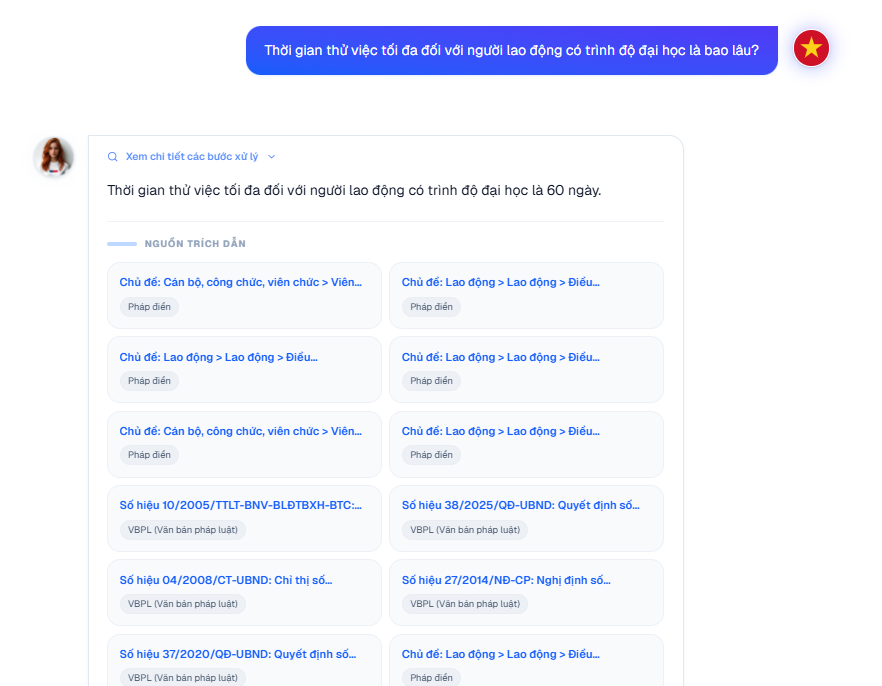
\includegraphics[width=0.65\textwidth]{pictures/chat-ui-image.png}

\refstepcounter{figure}
\textbf{Hình \thefigure:} Giao diện phản hồi câu hỏi về thời gian thử việc của hệ thống
\label{fig:chat_ui_probation}
\end{figure}

\begin{figure}[H]
\centering
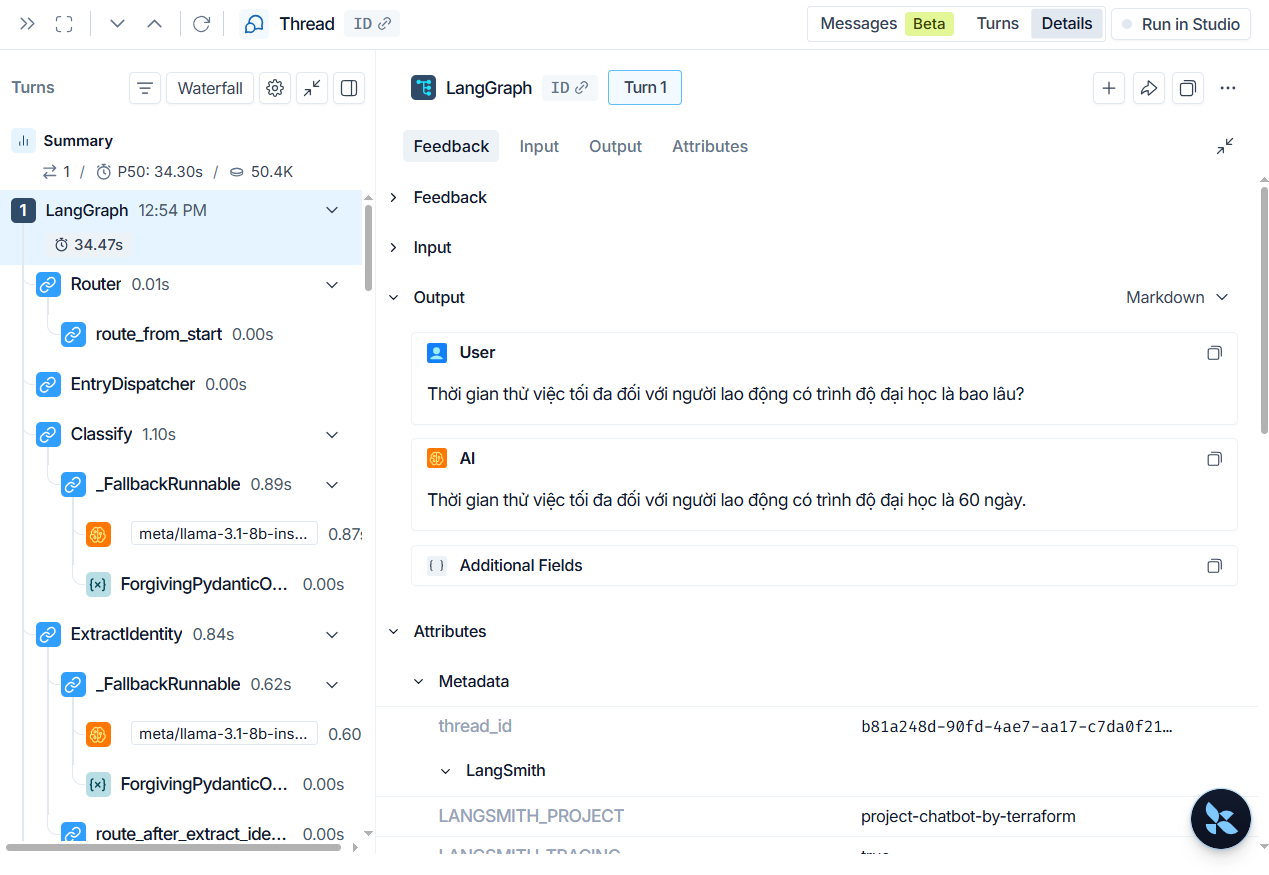
\includegraphics[width=0.65\textwidth]{pictures/langsmith-image-32.png}

\refstepcounter{figure}
\textbf{Hình \thefigure:} Chi tiết LangSmith về thời gian thử việc
\label{fig:langsmith_probation}
\end{figure}

% \newpage
% ==========================================
% Câu hỏi 2: Lực hấp dẫn
% ==========================================
% \vspace{1em}
\noindent\textbf{Câu hỏi:} Công thức tính lực hấp dẫn trong vật lý lượng tử là gì? \\
\textbf{Link:} \url{https://20206205.tech/share/d51942b0-0aff-4ead-88ae-e813c47a9a9c/2f96a259}

\begin{figure}[H]
\centering
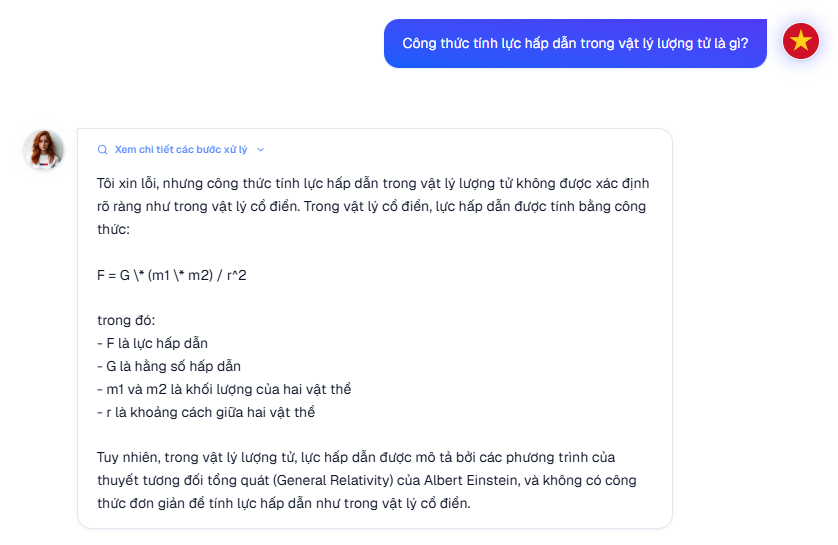
\includegraphics[width=0.65\textwidth]{pictures/chat-ui-image-1.png}

\refstepcounter{figure}
\textbf{Hình \thefigure:} Giao diện phản hồi câu hỏi về lực hấp dẫn trong vật lý lượng tử
\label{fig:chat_ui_gravity}
\end{figure}

\begin{figure}[H]
\centering
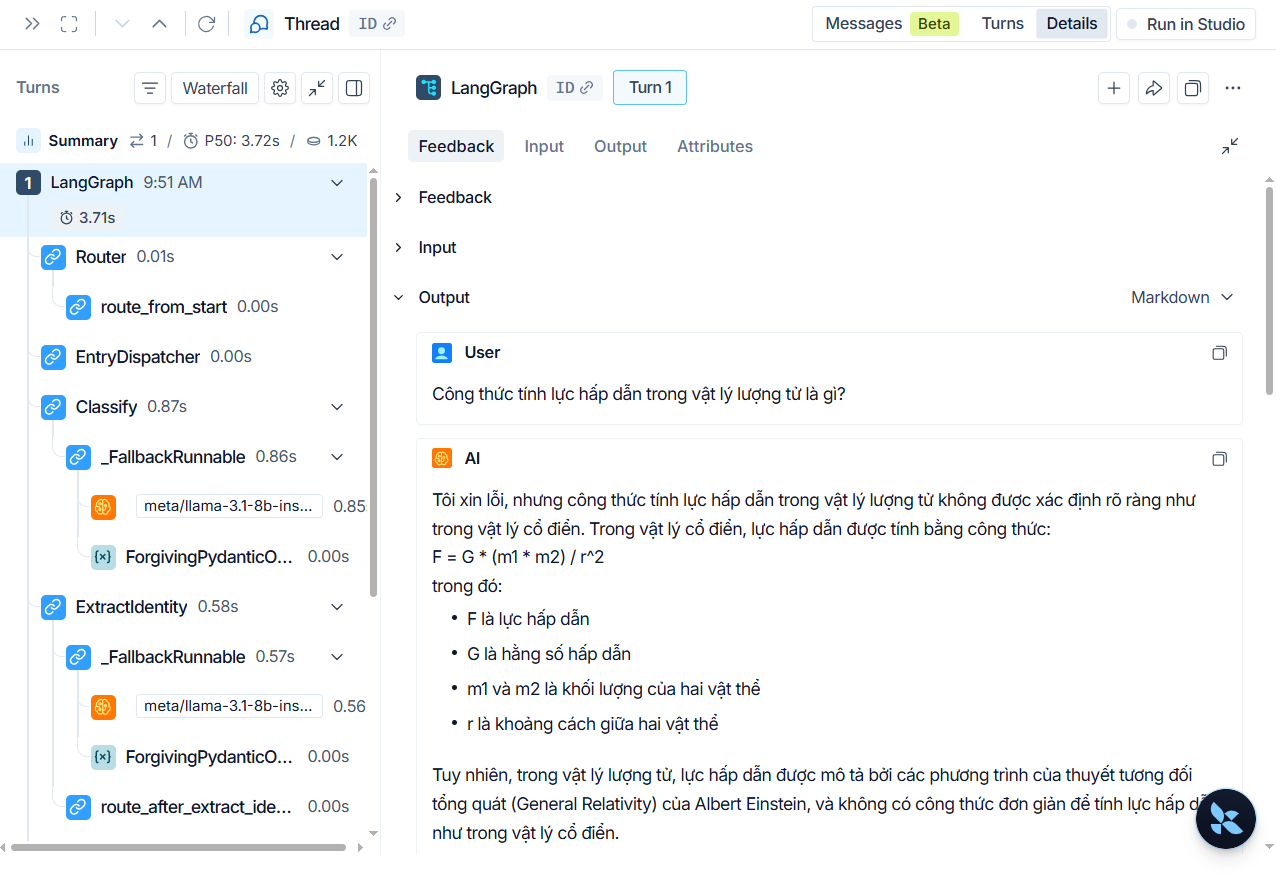
\includegraphics[width=0.65\textwidth]{pictures/langsmith-image-6.png}

\refstepcounter{figure}
\textbf{Hình \thefigure:} Chi tiết LangSmith về lực hấp dẫn
\label{fig:langsmith_gravity}
\end{figure}

% \newpage
% ==========================================
% Câu hỏi 3: Thuế thu nhập cá nhân
% ==========================================
% \vspace{1em}
\noindent\textbf{Câu hỏi:} Theo luật mới, sinh viên đi làm thêm không cần đóng thuế thu nhập cá nhân đúng không? \\
\textbf{Link:} \url{https://20206205.tech/share/0a65a3ff-e2e9-4943-920a-483fab52bfc8/eade4ab7}

\begin{figure}[H]
\centering
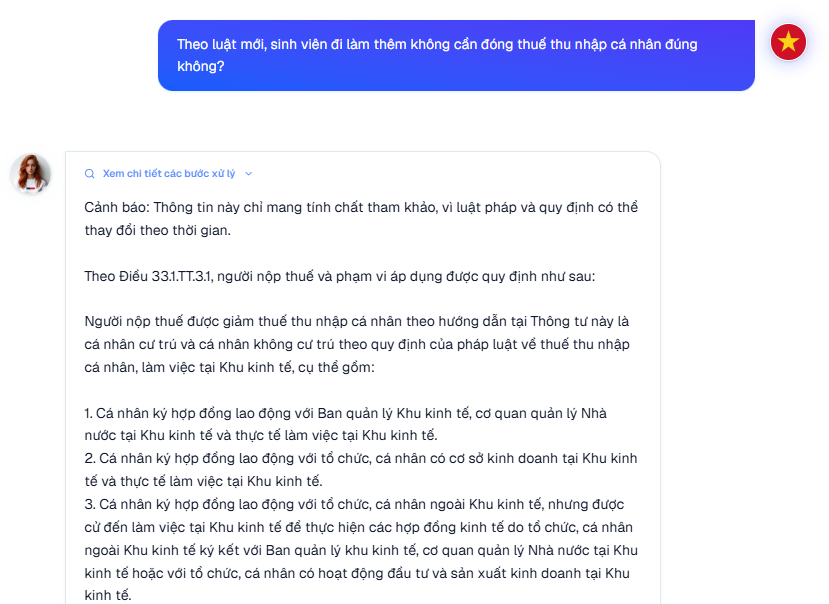
\includegraphics[width=0.65\textwidth]{pictures/chat-ui-image-4.png}

\refstepcounter{figure}
\textbf{Hình \thefigure:} Giao diện phản hồi câu hỏi về thuế thu nhập cá nhân của sinh viên đi làm thêm
\label{fig:chat_ui_tax}
\end{figure}

\begin{figure}[H]
\centering
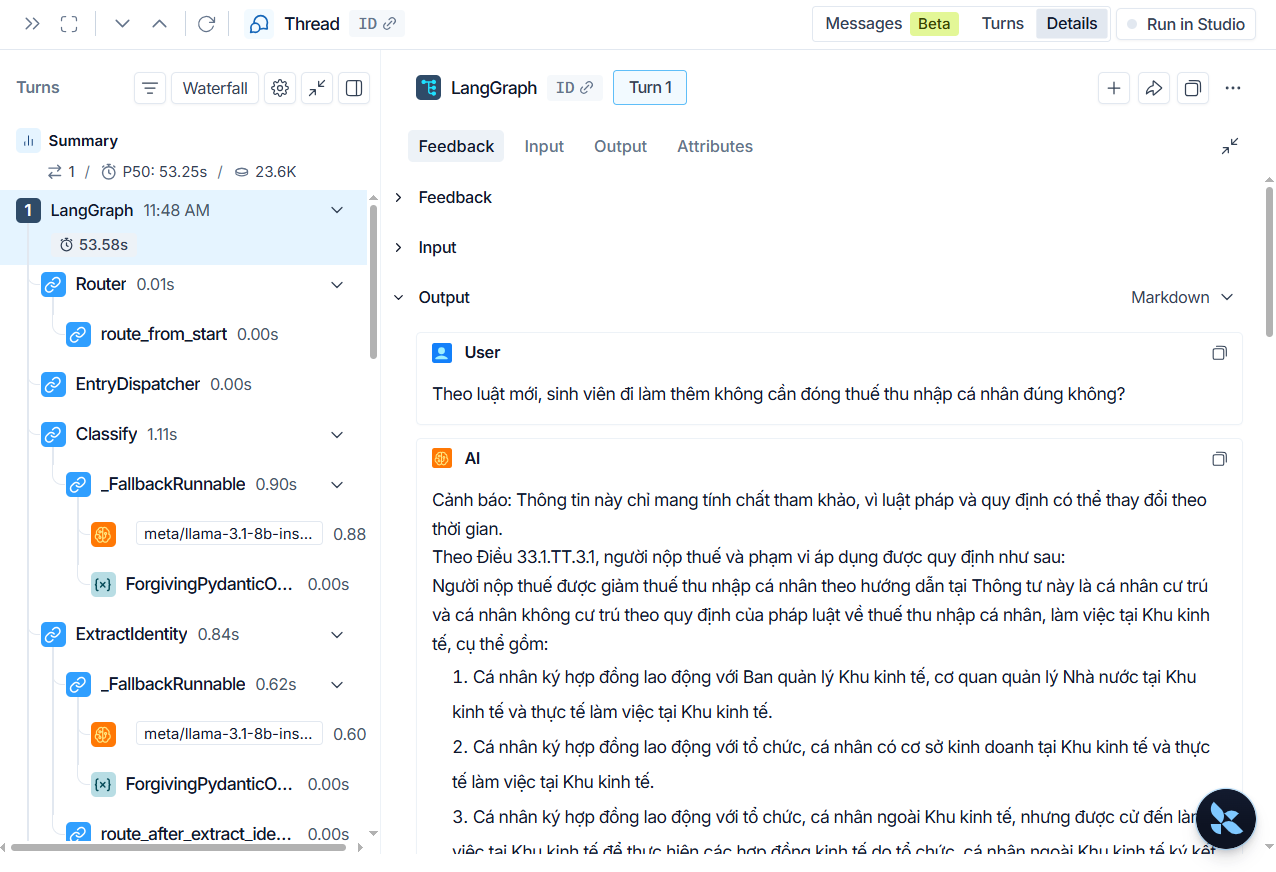
\includegraphics[width=0.65\textwidth]{pictures/langsmith-image-7.png}

\refstepcounter{figure}
\textbf{Hình \thefigure:} Chi tiết LangSmith về thuế thu nhập cá nhân
\label{fig:langsmith_tax}
\end{figure}

% \newpage
% ==========================================
% Câu hỏi 4: Đăng ký thuế
% ==========================================
% \vspace{1em}
\noindent\textbf{Câu hỏi:} Làm sao để đăng ký cái đó? \\
\textbf{Link:} \url{https://20206205.tech/share/8dc3c4e1-b63d-4d70-98f7-a89bfacefadc/2d022228}

\begin{figure}[H]
\centering
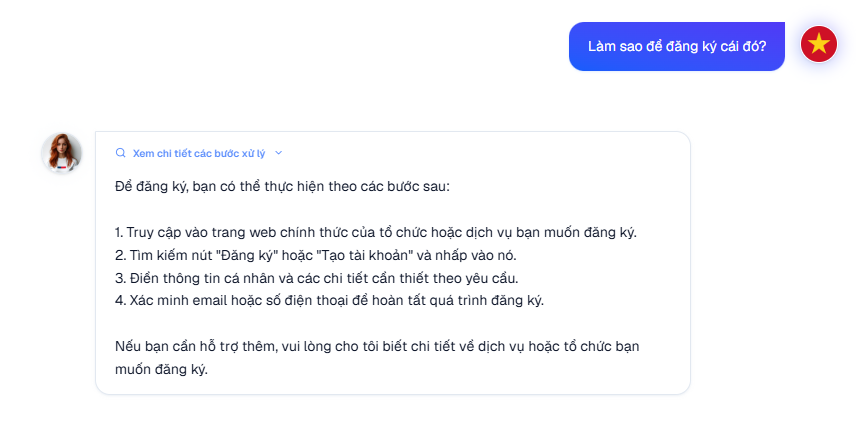
\includegraphics[width=0.9\textwidth]{pictures/chat-ui-image-2.png}

\refstepcounter{figure}
\textbf{Hình \thefigure:} Giao diện phản hồi câu hỏi tiếp nối về cách thức đăng ký
\label{fig:chat_ui_register}
\end{figure}

\begin{figure}[H]
\centering
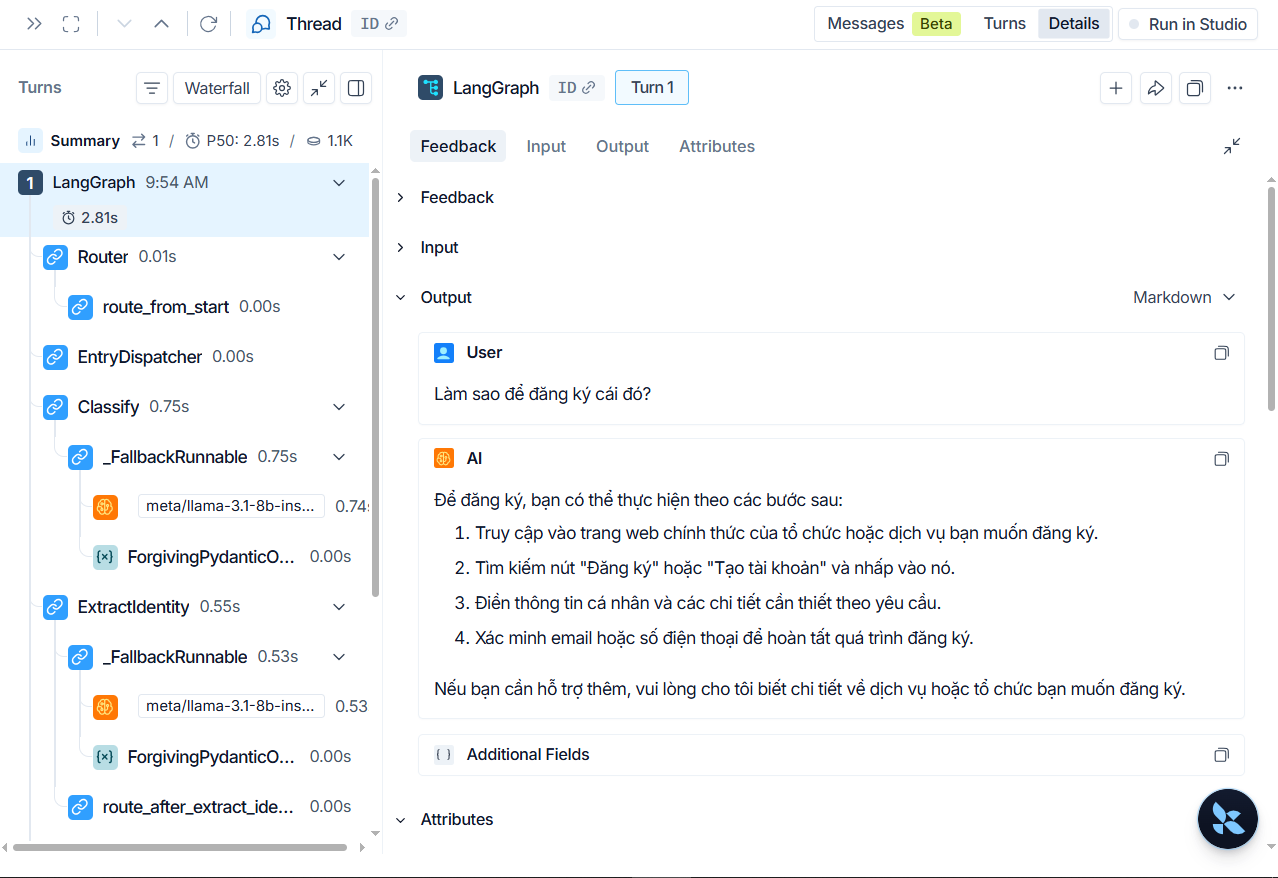
\includegraphics[width=0.65\textwidth]{pictures/langsmith-image-8.png}

\refstepcounter{figure}
\textbf{Hình \thefigure:} Chi tiết LangSmith về cách thức đăng ký
\label{fig:langsmith_register}
\end{figure}

% \newpage
% ==========================================
% Câu hỏi 5: Chấm dứt hợp đồng lao động
% ==========================================
% \vspace{1em}
\noindent\textbf{Câu hỏi:} Người lao động đơn phương chấm dứt hợp đồng lao động xác định thời hạn cần báo trước bao nhiêu ngày? \\
\textbf{Link:} \url{https://20206205.tech/share/80a989ad-6b2e-46b6-84ec-baf843c70e14/0fcaa121}

\begin{figure}[H]
\centering
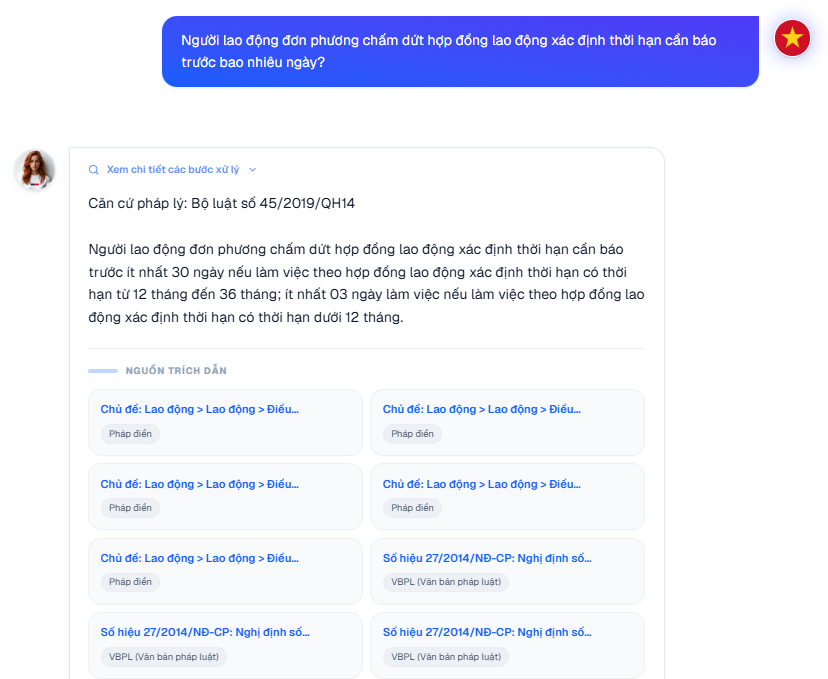
\includegraphics[width=0.65\textwidth]{pictures/chat-ui-image-5.png}

\refstepcounter{figure}
\textbf{Hình \thefigure:} Giao diện phản hồi câu hỏi về chấm dứt hợp đồng lao động
\label{fig:chat_ui_terminate_contract}
\end{figure}

\begin{figure}[H]
\centering
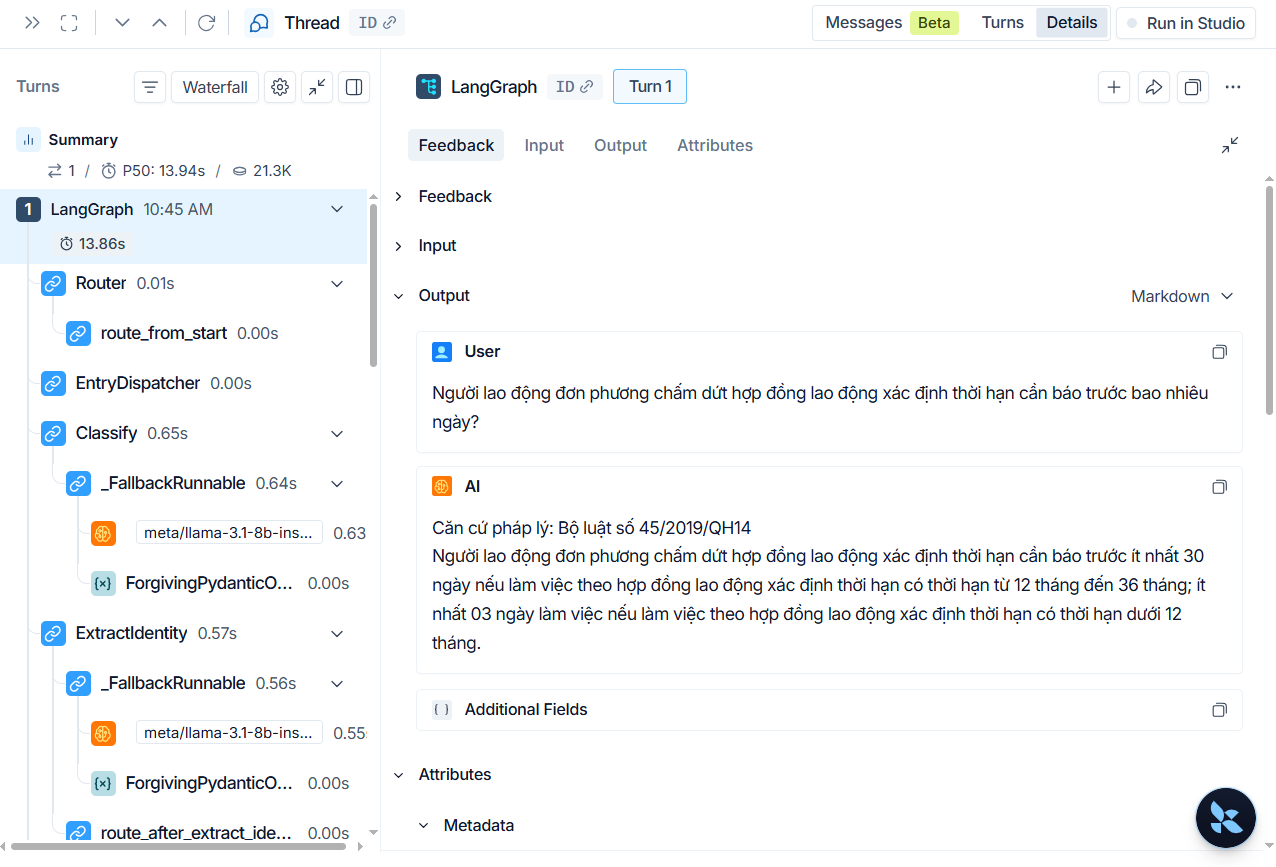
\includegraphics[width=0.65\textwidth]{pictures/langsmith-image-9.png}

\refstepcounter{figure}
\textbf{Hình \thefigure:} Chi tiết LangSmith về chấm dứt hợp đồng lao động
\label{fig:langsmith_terminate_contract}
\end{figure}

\newpage

\vspace*{\fill}
\begin{center}
% Trang này chỉ để trống!
\thispagestyle{empty}
\end{center}
\vspace*{\fill}

\newpage

%%%%%%%%%%%%%%%%%%%%%%%%%%%%%%%%%%%%%%%%%%%%%%%%%%%%%%%
\ifdev
\newpage

{
\color{RedHUST}
Chữ tạm màu đỏ

Dòng thứ hai vẫn có màu đỏ và không bị lỗi ngắt đoạn.
}

\url{https://example.com}

\begin{figure}[H]
\centering

\includegraphics[scale = 0.2]{pictures/LogoHust.png}
\caption{Logo của Đại học Bách Khoa Hà Nội 1}
\end{figure}

\begin{figure}[H]
\centering

\includegraphics[width=0.1\textwidth]{pictures/LogoHust.png}
\caption{Logo của Đại học Bách Khoa Hà Nội 2}
\end{figure}

\begin{itemize}
\item Nội dung mục 1
\item Chấm màu xanh
\end{itemize}

\textit{In nghiêng đoạn văn bản}

\textbf{In đậm đoạn văn bản}

\begin{block}{Ứng dụng trong đồ án}
Nội dung block
\end{block}

\lipsum[1]

\enquote{Đây là văn bản đặc biệt}

\newpage

\fi

\fi

\end{document}
